%------------------------------------------------------------------------------------------
% Meta-commands for the TeXworks editor
%
% !TEX encoding = UTF-8
% !TEX program = pdflatex
%------------------------------------------------------------------------------------------

%------------------------------------------------------------------------------------------
% INITIAL DEFINITIONS
%------------------------------------------------------------------------------------------

%******************************************************************************************
%
% AUTHOR:           Agostino De Marco
% DESCRIPTION:      This is "_init.tex", containing plain TeX commands.
%                   Goes in document before \documentclass
%
%******************************************************************************************
%
%------------------------------------------------------------------------------------------
% Meta-commands for the TeXworks editor
%
% !TeX root = ./Tesi.tex
% !TEX encoding = UTF-8
% !TEX program = pdflatex
%------------------------------------------------------------------------------------------

%%% We need a non standard MakeIndex style, because many entries in
%%% the index have names containing `@'.  Compilation of the index
%%% requires the call `makeindex Tesi'

\begin{filecontents*}{Tesi.ist}
actual '='
\end{filecontents*}

%%% Some constant strings

\def\myAuthorsList{Lorenzo~Attanasio}
\def\myAuthorListAbbreviated{L.~Attanasio}

\def\myDocName{Development of a Java Application for Parametric Aircraft Design}
\def\myDocSubTitle{A Master Thesis in Aerospace Engineering}

\def\myFooterLeft{\myAuthorsList\  -- \myDocName}
\def\myFooterRight{\myDocSubTitle}

\def\myDocVersion{ver.~2014.a}% <================== %?[ADJUST-HERE] EDIT THIS STRING AS NEEDED
\def\myDocDate{November~2014}% not used

%% EOF


%------------------------------------------------------------------------------------------
% LaTeX STARTING DECLARATION
%------------------------------------------------------------------------------------------

\documentclass[12pt,oneside]{book}

%------------------------------------------------------------------------------------------
% PREAMBLE
%------------------------------------------------------------------------------------------

%******************************************************************************************
%
% AUTHOR:           Agostino De Marco
% DESCRIPTION:      This is "_preamble.tex" file, included by the master source file
%                   "Tesi.tex".
%
%******************************************************************************************

%------------------------------------------------------------------------------------------
% Meta-commands for the TeXworks editor
%
% !TeX root = ./Tesi.tex
% !TEX encoding = UTF-8
% !TEX program = pdflatex

%------------------------------------------------------------------------------------------
% page layout with geometry (see layout_geometry_test.tex)
\usepackage[
    % driver=none,% needed with the crop package
%    papersize = a4paper,
	paperwidth = 210mm,
	paperheight = 297mm,
    % papersize={7in,10in},
    %papersize={8in,10in},% CreateSpace industry standard
    %papersize={8.5in,11in},% CreateSpace industry standard
    % papersize={258mm,201mm}, % Metric Large Crown Quarto, see: http://www.prepressure.com/library/paper-sizes
    hmargin={1.75cm,0.90cm},vmargin={1cm,1.8cm},marginparwidth=2.6cm,
    includehead,
%    includefoot,
%    footskip=1.6cm,
    includemp
    ]{geometry}
    
\usepackage{needspace}
\usepackage{pdflscape}

% \usepackage[cam,a4,center]{crop}

%------------------------------------------------------------------------------------------
% Language and encoding

\usepackage[utf8]{inputenc}
\usepackage[english,italian]{babel}
\usepackage{csquotes}% Recommended with biblatex combined with italian (as main language)

%------------------------------------------------------------------------------------------
% LaTeX3 stuff

\usepackage{expl3}

%------------------------------------------------------------------------------------------
% manage date and time

\usepackage[short,nodayofweek,12hr]{datetime}

%-------------------------------------------------------------------------------------
% Mathematics and related stuff

\usepackage{amsmath}
%\usepackage%
%   %[intlimits]
%   {amsmath}
%\usepackage{amsfonts}
%\usepackage{amsbsy}
%\usepackage{fixmath}
\usepackage{mathtools}
\usepackage{cancel}

%-------------------------------------------------------------------------------------
% Fonts and related stuff

\usepackage[T1]{fontenc}
\usepackage[final]{microtype}

\usepackage{relsize}% font relative sizing commands

%\usepackage{newtxtext}% replaces the txfonts package;
%\usepackage[varg]{newtxmath}

% MathTime Professional 2

%\renewcommand{\rmdefault}{ptm}      % set Times as the default text font
%\usepackage{libertine}% \copyright symbol unavailable
\usepackage{newtxtext}

% The following loads mtpro and defines some common MTPro options [2, 4]
\usepackage[subscriptcorrection,slantedGreek,nofontinfo,%
            mtpcal,%
            mtphbi %% mtpbbi
            ]{mtpro2}

% Options for blackboard bold fonts [2.9]:
%   mtphrb - holey roman bold        mtpbb - blackboard bold
%   mtphrd - holey roman bold dark   mtpbbd - blackboard bold dark
%   mtphbi - holey bold italic       mtpbbi - blackboard bold italic

% Options for alternate character sets [2.6, 2.7]:
%   mtpcal - assigns Math Script to the math alphabets \mathcal and \mathbcal,
%   overwriting the default math calligraphic typeface
%   mtpccal - assigns Math Curly to the math alphabets \mathcal and \mathbcal,
%   overwriting the default math calligraphic typeface
%   mtpscr - assigns Math Script to the new math alphabets \mathscr and \mathbscr,
%       leaving \mathcal unchanged
%   mtpfrak - assigns Math Fraktur to a new math alphabet \mathfrak

% Options for AMS symbols
%   amssymbols - makes the mtpro2 AMS symbols available

% Optionally load the following package to use heavy symbols in place of bold symbols
%\usepackage{bm}

% font for Aspect Ratio

\usepackage%
   [TM]% NOTE: needs version 2012 _and_ fonts/tfm/public/aspectratio/*.tfm
   {ar}% original package by Claudio Beccari (based on Computer Modern Roman)
%
%\usepackage{my-ar-tm}% AR ligature based on Times font design
%\newcommand{\AR}{{\ARtm}}
%\newcommand{\ARb}{{\ARtmb}}

\usepackage{textcomp}% additional glyphs
\usepackage{pifont} % for dingbats
\usepackage{marvosym} % for \Keyboard, etc

% Define text sans-serif font
% --> package txfonts uses Helvetica
\usepackage%
   [scaled=0.90]{helvet}% scale Helvetica as appropriate
   %[scaled=0.95]{berasans}% alternative to Helvetica

% Define text mono-spaced font
% --> package txfonts uses TX mono (monospace typewriter font)
\usepackage%
   [scaled=0.825]% 0.865 , 0.84
   {beramono}% set bera as mono-spaced font family

%\usepackage{enumitem}
%\setlist{noitemsep} % or \setlist{nosep} to leave space around whole list
\renewcommand{\labelitemi}{\small$\bullet$}
\newcommand{\smallspacing}{0.1em}
\newcommand{\medspacing}{0.15em}
	
%------------------------------------------------------------------------------------------
% FRONTESPIZIO by Enrico Gregorio
\usepackage{frontespizio}

%------------------------------------------------------------------------------------------
% Theorem-like stuff

%
\usepackage[amsmath,hyperref]{ntheorem}% NB: deve essere caricato DOPO babel

% definisce uno stile di teorema ad header vuoto
% richiede ntheorem.sty
\makeatletter
  \newtheoremstyle{mytheoremstyle}
    {\item[]}%
    {\item[]}
\makeatother
\theoremstyle{mytheoremstyle}% <------  seleziona lo stile appena definito
%\theoremstyle{margin}       %          ... altri stili predefiniti in ntheorem
%\theoremstyle{nonumberplain}

% nuovo theorem-like environment
\newtheorem{myExampleT}{}[chapter]

% myExample label & format
\newcommand\myExampleLabel{Esempio}
\newcommand\myExampleLabelFormat{%
    \textbf{\upshape\hspace{3pt}\myExampleLabel\ \themyExampleT}%
}
\newcommand\myExampleMarkPencilKeyboardMouse{%
    \bf\ding{46}\ \raisebox{-2pt}[0pt][0pt]{\relsize{4}\Keyboard\hspace{2pt}\ComputerMouse}%
}
\newcommand\myExampleMarkKeyboardMouse{%
    \raisebox{-2pt}[0pt][0pt]{\relsize{4}\Keyboard\hspace{2pt}\ComputerMouse}%
}
\newcommand\myExampleEndMark{%
    {\ding{118}}% \ding{111}
}

% environment per gli Esempi
\newenvironment{myExample}[1][\ding{46}]{%
    %###########################################################
    % eseguito all'inizio dell'environment
    %###########################################################
    \begin{myExampleT}%
    \adjustbox{set height=1.1\baselineskip,set depth=0.5\baselineskip,valign=m,%
        center=\linewidth,bgcolor=mylightblue!50}{%
        \adjustbox{left=0.6\linewidth}{%
            \myExampleLabelFormat%
        }%
        \adjustbox{right=0.4\linewidth}{%
            #1\ %
        }%
    }%
    \medskip
    \par\upshape% testo normale
}{%
    %###########################################################
    % eseguito alla fine dell'environment
    %###########################################################
    \end{myExampleT}%
    \smallskip
    \adjustbox{set height=0.55\baselineskip,set depth=0.11\baselineskip,valign=m,%
        center=\linewidth,bgcolor=mylightblue!50}{\relsize{-2}\myExampleEndMark}
    \medskip
}%

% nuovo theorem-like environment
%\newtheorem{myExampleTX}{}[chapter]

% environment per gli Esempi esteso (X)
%\makeatletter
\newenvironment{myExampleX}[2]{% accetta due argomenti: #1 titolo, #2 simbolo nell'header
    %###########################################################
    % ciò che viene eseguito all'inizio dell'environment
    %###########################################################
    \begin{myExampleT}
    %\stepcounter{myexamplecounter}% incrementa il contatore
    \par\vskip 8pt% a capo e skip verticale
    \noindent
    % striscia colorata
    \makebox[0em][l]{%
        {\color{mylightblue!50}\rule[-8pt]{\textwidth}{1.8em}}%
    }%
    % scritta
    \makebox[1.0\textwidth][c]{%
        %{\myExampleLabelFormat}%
        \textbf{\upshape\hspace{3pt}\myExampleLabel\ \themyExampleT:}\quad\textit{#1}\hfill\textbf{#2\ }%
    }%
    \vskip 8pt% recupera gli 8pt di \rule[-8pt]
    \smallskip%
    %\noindent%
    \upshape% testo normale
}{%
    %###########################################################
    % ciò che viene eseguito alla fine dell'environment
    %###########################################################
    %\addvspace{3.2ex plus 0.8ex minus 0.2ex}%
    \end{myExampleT}
    %\par\vskip 2pt
    \noindent
    \smallskip
    % striscia colorata
    \makebox[0em][l]{%
        {\color{mylightblue!50}\rule%
                            [0pt]%[-9pt]%
                            {\textwidth}{0.6em}}% 1.8em
    }%
    % simbolo di chiusura
    \makebox[1.0\textwidth][c]{%
        %{\raisebox{7pt}{\myExampleEndMark}}
        {\raisebox{0.6pt}{\relsize{-2}\myExampleEndMark}}
    }%
    %\par\vskip-2pt%
    %\noindent
    \medskip
}%

%.................................................. Matlab Tip
% nuovo theorem-like environment
\newtheorem{myMatlabTipT}{}[chapter]

% myExample label & format
\newcommand\myMatlabTipLabel{Matlab {\itshape tip}}
\newcommand\myMatlabTipLabelFormat{%
    \textbf{\upshape\hspace{3pt}\myMatlabTipLabel\ \themyMatlabTipT}%
}

\newcommand\myMatlabTipKeyboardMouse{%
    \raisebox{-2pt}[0pt][0pt]{\relsize{4}\Keyboard\hspace{2pt}\ComputerMouse}%
}

\newcommand\myMatlabTipEndMark{%
    {\ding{118}}% \ding{111}%
}

% environment per gli Esempi
%\makeatletter
\newenvironment{myMatlabTip}[1][\myMatlabTipKeyboardMouse]{%  \ding{46}
    %###########################################################
    % ciò che viene eseguito all'inizio dell'environment
    %###########################################################
    \begin{myMatlabTipT}%
    \adjustbox{set height=1.1\baselineskip,set depth=0.5\baselineskip,valign=m,%
        center=\linewidth,bgcolor=mylightblue!50}{%
        \adjustbox{left=0.6\linewidth}{%
            \myMatlabTipLabelFormat%
        }%
        \adjustbox{right=0.4\linewidth}{%
            #1\ %
        }%
    }%
%
    \par\upshape% testo normale
    \smallskip%
}{%
    %###########################################################
    % ciò che viene eseguito alla fine dell'environment
    %###########################################################
    %\addvspace{3.2ex plus 0.8ex minus 0.2ex}%
    \end{myMatlabTipT}
%    %\par\vskip 2pt
    \par\noindent%\smallskip
    \adjustbox{set height=0.55\baselineskip,set depth=0.11\baselineskip,valign=m,%
        center=\linewidth,bgcolor=mylightblue!50}{\relsize{-2}\myExampleEndMark}
    \medskip
}%


% environment per gli Esercizi esteso (X)
%\makeatletter

% nuovo theorem-like environment
\newtheorem{myExerciseT}{}[chapter]

\newcommand\myExerciseEndMark{%
    {\ding{118}}% \ding{111}
}

% myExercise label & format
\newcommand\myExerciseLabel{Esercizio}
\newcommand\myExerciseLabelFormat{%
    %\textbf{\bf\ding{46}\ \myExampleLabel\ \themyExampleT}
    \textbf{\upshape\hspace{3pt}\myExampleLabel\ \themyExampleT}%
    \hfill\textbf{\bf\ding{46}\ \raisebox{-2pt}[0pt][0pt]{\relsize{4}\Keyboard\hspace{2pt}\ComputerMouse}\ }%
}

\newenvironment{myExerciseX}[2]{% accetta due argomenti: #1 titolo, #2 simbolo nell'header
    %###########################################################
    % ciò che viene eseguito all'inizio dell'environment
    %###########################################################
    \begin{myExerciseT}
    %\stepcounter{myexamplecounter}% incrementa il contatore
    \par\vskip 8pt% a capo e skip verticale
    \noindent
    % striscia colorata
    \makebox[0em][l]{%
        {\color{mylightblue!50}\rule[-8pt]{\textwidth}{1.8em}}%
    }%
    % scritta
    \makebox[1.0\textwidth][c]{%
        %{\myExampleLabelFormat}%
        \textbf{\upshape\hspace{3pt}\myExerciseLabel\ \themyExerciseT:}\quad\textit{#1}\hfill\textbf{#2\ }%
    }%
    \vskip 8pt% recupera gli 8pt di \rule[-8pt]
    \smallskip%
    %\noindent%
    \upshape% testo normale
}{%
    %###########################################################
    % ciò che viene eseguito alla fine dell'environment
    %###########################################################
    %\addvspace{3.2ex plus 0.8ex minus 0.2ex}%
    \end{myExerciseT}
    %\par\vskip 2pt
    \noindent
    \smallskip
    % striscia colorata
    \makebox[0em][l]{%
        {\color{mylightblue!50}\rule%
                            [0pt]%[-9pt]%
                            {\textwidth}{0.6em}}% 1.8em
    }%
    % simbolo di chiusura
    \makebox[1.0\textwidth][c]{%
        %{\raisebox{7pt}{\myExampleEndMark}}
        {\raisebox{0.6pt}{\relsize{-2}\myExerciseEndMark}}
    }%
    %\par\vskip-2pt%
    %\noindent
    \medskip
}%
%\makeatother

%%%\usepackage{amsthm}
%%%
%%% http://www.guit.sssup.it/phpbb/viewtopic.php?t=3523&highlight=ntheorem
%%% http://www.tug.org/tutorials/tugindia/chap17-prn.pdf

%%%\makeatletter
%%%\def\@thm#1#2#3{%
%%%  \ifhmode\unskip\unskip\par\fi
%%%  \normalfont
%%%  \trivlist
%%%  \let\thmheadnl\relax
%%%  \let\thm@swap\@gobble
%%%  \thm@notefont{\fontseries\bfdefault\upshape}%
%%%  \thm@headpunct{.}% add period after heading
%%%  \thm@headsep 5\p@ plus\p@ minus\p@\relax
%%%  \thm@space@setup
%%%  #1% style overrides
%%%  \@topsep \thm@preskip               % used by thm head
%%%  \@topsepadd \thm@postskip           % used by \@endparenv
%%%  \def\@tempa{#2}\ifx\@empty\@tempa
%%%    \def\@tempa{\@oparg{\@begintheorem{#3}{}}[]}%
%%%  \else
%%%    \refstepcounter{#2}%
%%%    \def\@tempa{\@oparg{\@begintheorem{#3}{\csname the#2\endcsname}}[]}%
%%%  \fi
%%%  \@tempa
%%%}
%%%\makeatother
%%%
%%%\newtheorem{myExampleSimple}{Esempio}[chapter]

\usepackage[hyphens]{url}

%------------------------------------------------------------------------------------------
% Management of floating material

\usepackage{float}
   % I got this somewhere on the net:
   \renewcommand{\textfraction}{0.15}
   \renewcommand{\topfraction}{0.85}
   \renewcommand{\bottomfraction}{0.65}
   \renewcommand{\floatpagefraction}{0.60}

% \usepackage[maxfloats=19]{morefloats}[2012/01/28]% v1.0f
\usepackage{morefloats}
   
\usepackage{placeins}

\usepackage{caption}
\captionsetup[figure]{
    %format=hang,%
    labelsep=space,%
    font=small,labelfont={bf,sf,small},%
    %justification=raggedright,%
    singlelinecheck=true%,%
    %width=1.1\textwidth%%
}
\captionsetup[table]{
    %format=hang,%
    labelsep=space,%
    font=small,labelfont={bf,sf,small},%bf,%
    justification=raggedright,%
    singlelinecheck=true,%
    %width=0.8\textwidth,%
    belowskip=0.5em%
}
\captionsetup[lstlisting]{
    %format=hang,%
    labelsep=space,%
    font=small,labelfont={bf,sf,small},%
    %justification=raggedright,%
    singlelinecheck=true%,%
    %width=1.1\textwidth%%
}

\captionsetup[ctable]{
    %format=hang,%
    labelsep=space,%
    font=small,labelfont={sf,bf,small},% bf
    %justification=raggedright,%
    singlelinecheck=true,%
    width=0.8\textwidth,%
    belowskip=0.5em%
}

%% see here: http://tex.stackexchange.com/questions/13625/subcaption-vs-subfig
%\usepackage{subfig}
\usepackage{subcaption}% multiple figures in one floating object 
% subcaption CANNOT BE USED IN COOPOEARTION WITH SUBFIG
\usepackage[innercaption,wide]{sidecap}

%------------------------------------------------------------------------------------------
% Graphics and related stuff
\usepackage{graphicx}
\graphicspath{{images/}}
\usepackage[export]{adjustbox}
\usepackage{tikz}
\usepackage{pgfplots}
\pgfplotsset{compat=1.10}
\usepackage{wrapfig}


%\usepackage{ifluatex}
%\ifluatex
%\usepackage{pdftexcmds}
%\makeatletter
%\let\pdfstrcmp\pdf@strcmp
%\let\pdffilemoddate\pdf@filemoddate
%\makeatother
%\fi

%% svg might be incompatible with subcaption
%\usepackage{svg}
%\setsvg{inkscape={"C:/Program Files (x86)/inkscape-0.48.5/inkscape.exe"= -z -C}}
%\setsvg{convert={"C:/Program Files/ImageMagick-6.9.0-Q16/convert.exe" -density 300}}
%\setsvg{pdftops={"C:/Program Files/xpdfbin-win-3.04/bin64/pdftops.exe" -eps}}

%\newcommand{\executeiffilenewer}[3]{%
%	\ifnum\pdfstrcmp%
%	{\pdffilemoddate{#1}}%
%	{\pdffilemoddate{#2}}%
%	>0%
%	{\immediate\write18{#3}}%
%	\fi%
%}
%\newcommand{\includesvg}[2][]{%
%	\executeiffilenewer{#1#2.svg}{#1#2.pdf}%
%	{inkscape.exe -z -D --file=#1#2.svg --export-pdf=#1#2.pdf --export-latex}%
%	\subimport{#1}{#2.pdf_tex}%
%}

%\usepackage{transparent}
\newlength\figureheight
\newlength\figurewidth
\usepackage{relsize}
\tikzset{
	master/.style={
		execute at end picture={
			\coordinate (lower right) at (current bounding box.south east);
			\coordinate (upper left) at (current bounding box.north west);
		}
	},
	slave/.style={
		execute at end picture={
			\pgfresetboundingbox
			\path (upper left) rectangle (lower right);
		}
	}
}

\usepackage{xcolor}
\usepackage{color}

\definecolor{black}{rgb}{0, 0, 0}
\definecolor{pblue}{rgb}{0.13,0.13,1}
\definecolor{pgreen}{rgb}{0,0.5,0}
\definecolor{pred}{rgb}{0.9,0,0}
\definecolor{pgrey}{rgb}{0.46,0.45,0.48}
\definecolor{mydarkgreen}{rgb}{0.03,0.47,0.03}
\definecolor{mydarkblue}{rgb}{0.07,0.08,0.4}
\definecolor{mylightblue}{rgb}{.8, .8, 1}
\definecolor{mylightgray}{rgb}{0.95,0.95,0.95}
\definecolor{mymidgray}{rgb}{0.85,0.85,0.85}
\definecolor{mydarkgray}{rgb}{0.35,0.35,0.35}
\definecolor{myblue}{rgb}{.4,.4,1}
\definecolor{colKeys}{rgb}{0,0,1}
\definecolor{colIdentifier}{rgb}{0,0,0}
\definecolor{colComments}{rgb}{0,0.5,1}
\definecolor{colString}{rgb}{0.6,0.1,0.1}

%\newcommand{\executeiffilenewer}[3]{%
%	\ifnum\pdfstrcmp%
%	{\pdffilemoddate{#1}}%
%	{\pdffilemoddate{#2}}%
%	>0%
%	{\immediate\write18{#3}}%
%	\fi%
%}
%
%\newcommand{\includesvg}[2][]{%
%	\executeiffilenewer{#1#2.svg}{#1#2.pdf}%
%	{inkscape-0.48.5.exe -z -D --file=#1#2.svg --export-pdf=#1#2.pdf --export-latex}%
%	\subimport{#1}{#2.pdf_tex}%
%}

%------------------------------------------------------------------------------------------
% Units of measure according to the SI standard

\usepackage{siunitx}
\sisetup{
  fixdp,dp=3,
  load=derived,
  unitsep=thin,
  valuesep=thin,
  decimalsymbol=comma,
  % digitsep=thin,
  % group-separator={},% ver. 2
  % sepfour=false,
  % round-mode = places,
  % round-precision = 3
}
%******************************************************************************************
%
% AUTHOR:           Agostino De Marco
% DESCRIPTION:      This is "_units.tex", an auxiliary LaTeX source file.
%                   Here we collect all customizations related to package siunitx
%                   (see _preamble.tex).
%
%******************************************************************************************

%------------------------------------------------------------------------------------------
% Meta-commands for the TeXworks editor
%
% !TeX root = ./Libro_MS.tex
% !TEX encoding = UTF-8
% !TEX program = pdflatex
%------------------------------------------------------------------------------------------

%-----------------------------------------------------------------------------------------------------
% siunitx ver 2.5 (July 2013 and later)
\usepackage%
  % [version-1-compatibility]%
  %[load-configurations = version-2]%
  {siunitx}
\sisetup{
  %load=derived,
  mode=math,
  inter-unit-product = {\,}, % unitsep=thin,
  number-unit-product = {\,}, % valuesep=thin,
  output-decimal-marker = {.}, % decimalsymbol=comma,% for European convention
  round-mode = places,
  exponent-product = {\cdot}, % expproduct = cdot,
  % digitsep=thin,
  group-separator = {},% ver. 2
  group-four-digits = false % sepfour=false
}

\DeclareSIUnit\degree{\ensuremath{^\circ}}

\DeclareSIUnit\deg{deg}

\DeclareSIUnit\inch{in}
\DeclareSIUnit\foot{ft}
\DeclareSIUnit\feet{ft}
\DeclareSIUnit\lb{lb}
\DeclareSIUnit\lbm{lb\ensuremath{_\mathrm{m}}}
\DeclareSIUnit\lbf{lb\ensuremath{_\mathrm{f}}}
\DeclareSIUnit\slug{slug}
\DeclareSIUnit\rankine{\ensuremath{^\circ}R}
\DeclareSIUnit\fahrenheit{\ensuremath{^\circ}F}
\DeclareSIUnit\kilopond{kg\ensuremath{_\mathrm{f}}}
\DeclareSIUnit\kgf{kg\ensuremath{_\mathrm{f}}}
\DeclareSIUnit\knots{kts}

% load settings from ./_units.tex

%------------------------------------------------------------------------------------------
% Dummy text, provisional stuff

\usepackage{lipsum}
\usepackage{blindtext}

\usepackage[%
   backgroundcolor=orange!20,bordercolor=orange,
   shadow,
   textsize=footnotesize,
   colorinlistoftodos
   % ,disable % use this to disable the notes
   ]{todonotes}

\newcounter{todocounter}

\newcommand{\TODO}[2][]{%
   % initials of the author (optional) + note in the margin
   \refstepcounter{todocounter}%
   {%
      \setstretch{0.85}% line spacing
      \todo[backgroundcolor={orange!20},bordercolor=orange,size=\relsize{-1}]{%
         \sffamily%
         \thetodocounter.~\textbf{[\uppercase{#1}]:} #2%
      }%
   }}

\newcommand{\TODOInline}[2][]{%
   % initials of the author (optional) + note in the margin
   \refstepcounter{todocounter}%
   {%
      \setstretch{0.85}% line spacing
      \todo[inline,backgroundcolor={orange!20},bordercolor=orange,size=\relsize{-1}]{%
         \sffamily%
         \thetodocounter.~\textbf{[\uppercase{#1}]:}~#2%
      }%
   }}

%%% Examples of usage:
%%% \TODO[ADM]{Continue this section taking material from Stevend \& Lewis book.}
%%% \TODOInline[JSB]{Remove this sentence.}

\newcommand{\TODOInsertRef}[1]{\todo[color=green!40]{#1}}
\newcommand{\TODOExplainInDetail}[1]{\todo[color=red!40]{#1}}
\newcommand{\TODORewrite}[1]{\todo[color=yellow!40]{#1}}

%------------------------------------------------------------------------------------------
% Miscellaneous stuff

\usepackage{xspace}
\usepackage{calc}
\usepackage{ragged2e}
\usepackage[defblank]{paralist}
\usepackage{algorithmic}
\usepackage{multicol}
\usepackage{appendix}

% smart cross-referencing
\usepackage[italian]{varioref}
% Si veda "Breve guida ai pacchetti più usati" di Enrico Gregorio
% http://profs.sci.univr.it/~gregorio/breveguida.pdf
\makeatletter
\vref@addto\extrasitalian{\def\reftextfaraway#1{a pagina~\pageref{#1}}}
\makeatother


\usepackage{dcolumn}

\usepackage{ctable}
\usepackage{booktabs,colortbl}
\usepackage{tabularx}

%------------------------------------------------------------------------------------------
% Table of contents per chapter

\usepackage[english,tight]{minitoc}
\AtBeginDocument{%
    \addto\captionsitalian{\mtcselectlanguage{italian}}
}
%\mtcsetpagenumbers{secttoc}{off}
%\nostcpagenumbers

%------------------------------------------------------------------------------------------
% Advanced header and footer management

\usepackage[
            %sf,
            %bf,
            %compact,
            %topmarks,
            calcwidth,%
            pagestyles% loads titleps 
            ]{titlesec}

%\renewpagestyle{empty}[\small\sffamily]{
\renewpagestyle{empty}[\small]{
  \sethead{}{}{}
  \setfoot{}{}{}
}

%\renewpagestyle{plain}[\small\sffamily]{
\renewpagestyle{plain}[\small]{
  %\footrule
  \setfoot{}{\usepage}{}}

% needs \usepackage{calc} above
\widenhead*{0pt}{\marginparsep + \marginparwidth} % symmetrically
\renewpagestyle{plain}{}
%::::::::::::::::::::::::::::::::::::::::::::::::::::::::::::::::::::::::::::::::::::::::::
\newpagestyle{myBookPageStyle}[\bfseries\sffamily\footnotesize]{
    \headrule
    %\myColoredHeadrule% TO DO: got to define a colored line
    \sethead%
        [{\makebox[\marginparwidth+\marginparsep][l]{\thepage}%
            \ifnum\value{chapter}>0%
                {\chaptername}\ \thechapter\ \ {\sffamily\mdseries\chaptertitle}%
            \else {\sffamily\mdseries\chaptertitle}%
            \fi%
        }][][]
        {}{}{%
            \raggedleft%
            \ifnum\value{chapter}<1% e.g. in TOC chapter=0
                {\sffamily\mdseries\chaptertitle}%
            \else%
                \thesection\ \ {\sffamily\mdseries\sectiontitle}%
            \fi%
            {\makebox[\marginparwidth+\marginparsep][r]{\thepage}}%
        }
    % NOTE: this footer might become empty
    \footrule
    \setfoot%
        [][][\color{mydarkblue}\sf\scriptsize \myFooterLeft]% left-hand footer
        {\color{mydarkblue}\sf\scriptsize \myFooterRight}{}{}% right-hand footer
}
%::::::::::::::::::::::::::::::::::::::::::::::::::::::::::::::::::::::::::::::::::::::::::
\newpagestyle{myIndexPageStyle}[\bfseries\sffamily\footnotesize]{
    \headrule
    \sethead%
        [{\makebox[\marginparwidth+\marginparsep][l]{\thepage}%
            {\sffamily\mdseries Index}%
        }][][]
        {}{}{\raggedleft\thesection\ \ {\sffamily\mdseries\sectiontitle}{\makebox[\marginparwidth+\marginparsep][r]{\thepage}}}
    % NOTE: this footer might become empty
    %\footrule
    \setfoot%
        [][][\color{mydarkblue}\sf\scriptsize \myFooterLeft]% left-hand footer
        {\color{mydarkblue}\sf\scriptsize \myFooterRight}{}{}% right-hand footer
}
%::::::::::::::::::::::::::::::::::::::::::::::::::::::::::::::::::::::::::::::::::::::::::
\newpagestyle{myAppendixPageStyle}[\bfseries\sffamily\footnotesize]{
    \headrule
    \sethead%
        [{\makebox[\marginparwidth+\marginparsep][l]{\thepage}%
                {\chaptername}\ \thechapter\ \ {\sffamily\mdseries\chaptertitle}%
        }][][]
        {}{}{\raggedleft\thesection\ \ {\sffamily\mdseries\sectiontitle}{\makebox[\marginparwidth+\marginparsep][r]{\thepage}}}
    % NOTE: this footer might become empty
    %\footrule
    \setfoot%
        [][][\color{mydarkblue}\sf\scriptsize \myFooterLeft]% left-hand footer
        {\color{mydarkblue}\sf\scriptsize \myFooterRight}{}{}% right-hand footer
}
%::::::::::::::::::::::::::::::::::::::::::::::::::::::::::::::::::::::::::::::::::::::::::
\newpagestyle{myBibliographyPageStyle}[\bfseries\sffamily\footnotesize]{
    \headrule
    \sethead%
        [{\makebox[\marginparwidth+\marginparsep][l]{\thepage}%
            {\sffamily\mdseries Bibliografia}%
        }][][]
        {}{}{\raggedleft{\sffamily\mdseries Bibliografia}{\makebox[\marginparwidth+\marginparsep][r]{\thepage}}}
    % NOTE: this footer might become empty
    %\footrule
    \setfoot%
        [][][\color{mydarkblue}\sf\scriptsize \myFooterLeft]% left-hand footer
        {\color{mydarkblue}\sf\scriptsize \myFooterRight}{}{}% right-hand footer
}
%::::::::::::::::::::::::::::::::::::::::::::::::::::::::::::::::::::::::::::::::::::::::::
\newpagestyle{myGlossaryPageStyle}[\bfseries\sffamily\footnotesize]{
    \headrule
    \sethead%
        [{\makebox[\marginparwidth+\marginparsep][l]{\thepage}%
            {\sffamily\mdseries Glossary}%
        }][][]
        {}{}{\raggedleft\sffamily\mdseries Glossary\makebox[\marginparwidth+\marginparsep][r]{\thepage}}
    % NOTE: this footer might become empty
    %\footrule
    \setfoot%
        [][][\color{mydarkblue}\sf\scriptsize \myFooterLeft]% left-hand footer
        {\color{mydarkblue}\sf\scriptsize \myFooterRight}{}{}% right-hand footer
}
%::::::::::::::::::::::::::::::::::::::::::::::::::::::::::::::::::::::::::::::::::::::::::
\newpagestyle{myAcronymsPageStyle}[\bfseries\sffamily\footnotesize]{
    \headrule
    \sethead%
        [{\makebox[\marginparwidth+\marginparsep][l]{\thepage}%
            {\sffamily\mdseries Acronyms}%
        }][][]
        {}{}{\raggedleft\sffamily\mdseries Acronyms\makebox[\marginparwidth+\marginparsep][r]{\thepage}}
    % NOTE: this footer might become empty
    %\footrule
    \setfoot%
        [][][\color{mydarkblue}\sf\scriptsize \myFooterLeft]% left-hand footer
        {\color{mydarkblue}\sf\scriptsize \myFooterRight}{}{}% right-hand footer
}
%::::::::::::::::::::::::::::::::::::::::::::::::::::::::::::::::::::::::::::::::::::::::::
\newpagestyle{myListOfSymbolsPageStyle}[\bfseries\sffamily\footnotesize]{
    \headrule
    \sethead%
        [{\makebox[\marginparwidth+\marginparsep][l]{\thepage}%
            {\sffamily\mdseries List of symbols}%
        }][][]
        {}{}{\raggedleft\sffamily\mdseries List of symbols\makebox[\marginparwidth+\marginparsep][r]{\thepage}}
    % NOTE: this footer might become empty
    %\footrule
    \setfoot%
        [][][\color{mydarkblue}\sf\scriptsize \myFooterLeft]% left-hand footer
        {\color{mydarkblue}\sf\scriptsize \myFooterRight}{}{}% right-hand footer
}
%::::::::::::::::::::::::::::::::::::::::::::::::::::::::::::::::::::::::::::::::::::::::::
%::::::::::::::::::::::::::::::::::::::::::::::::::::::::::::::::::::::::::::::::::::::::::
%
% Set the initial style
%
\pagestyle{myBookPageStyle}

%% chapter head style via titlesec
\newcommand{\myChapterHeadingColorMix}{%
  %blue!65!black
  blue!0!black%
}
\newcommand{\myChapterHeadingColor}{\color{\myChapterHeadingColorMix}}

\titleformat{\chapter}[display]
    {\bfseries\Large}
    {%
        \myChapterHeadingColor% \color{blue!65!black}% color
        \filleft%
        %\Huge\chaptertitlename\ \thechapter%
        \minsizebox{!}{24pt}{\chaptertitlename}% needs package adjustbox
        \lapbox[0pt]{\width}{%
            \minsizebox{!}{40pt}{%
                %\ \fbox{\thechapter}
                \ \colorbox{\myChapterHeadingColorMix}{\color{white}\thechapter}% needs xcolor
            }%
        }% needs package adjustbox
    }
    {4ex}
    {{\color{gray!65!gray}\titlerule}
        \huge\bfseries\scshape
        \vspace{2ex}%
        \filright}
    [\vspace{2ex}%
        {\color{gray!65!gray}\titlerule}]

%------------------------------------------------------------------------------------------
% Advanced page margin management

\usepackage[strict]{changepage}% as of 2009
\usepackage{fullwidth}

%------------------------------------------------------------------------------------------
% Advanced graphics package

\usepackage{tikz}
\usetikzlibrary{calc}
\usetikzlibrary{positioning,trees,arrows}
\usetikzlibrary{fpu}

\usepackage{pgfplotstable}

% splittable boxes
\usepackage%
  [framemethod=tikz]%
  {mdframed}% texdoc.net/pkg/mdframed

\newcounter{myInsight}[chapter]

\global\mdfdefinestyle{InsightStyleDefault}{%
% Variant I
%    outerl inewidth=3pt,% works with tikz method
%    topline=true,%
%    linecolor=mydarkblue,%blue!20,%
%    innermargin=-13pt,
%    outermargin=-13pt,
%        %% WARNING: multicol is not supported in mdframed, otherwise you'd take a full span
%        % \dimexpr 2pt+3pt-13pt-\marginparsep-\marginparwidth\relax,
%    innerrightmargin=13pt,innerleftmargin=13pt,%
%    frametitlerule=true,frametitlerulecolor=mydarkblue,%blue!20,%
%    frametitlebackgroundcolor=mydarkblue,%blue!20,%
%    frametitlerulewidth=2pt%
%
% Variant II
    outerlinewidth=0pt,% 3pt,% works with tikz method
    middlelinewidth=0em,middlelinecolor=gray!60,
    hidealllines=true,
    topline=false,% true,%
    innermargin=-13pt,
    outermargin=-13pt,
        %% WARNING: multicol is not supported in mdframed, otherwise you'd take a full span
        % \dimexpr 2pt+3pt-13pt-\marginparsep-\marginparwidth\relax,
    innerrightmargin=13pt,innerleftmargin=13pt,%
    frametitlerule=true,%
    frametitlerulecolor=mydarkblue,%blue!20,%
    frametitlebackgroundcolor=mydarkblue,%blue!20,%
    frametitlerulewidth=0pt,% 2pt%
%%
   backgroundcolor=gray!15,
   middlelinecolor=gray!15,
   roundcorner=5pt,
   singleextra={%
      \fill[gray!60,rounded corners=2pt,] 
         ($(P)+(0,-2.05)$) -- ($(P)+(0.14,-0.55)$) --  ($(P)+(0.18,-0.25)$)
            [sharp corners] --  ($(P)+(0,-0.25)$) -- cycle ;
%
      \path let \p1=(P), \p2=(O) in ({(\x1-\x2)/2},\y2) coordinate (M) ;
      \shade[left color=gray!50,right color=gray!50,middle color=black!55,rounded corners] 
         ($(M)+(-0.51\linewidth,0)$) --
         ($(M)+(-0.51\linewidth,-0.135)$) -- ($(M)+(0,-0.055)$) 
            -- ($(M)+(0.51\linewidth,-0.135)$) -- ($(M)+(0.51\linewidth,0)$) ;
            % -- cycle ;
   },
   firstextra={%
      \fill[gray!60,rounded corners=2pt,] 
         ($(P)+(0,-2.05)$) -- ($(P)+(0.14,-0.55)$) --  ($(P)+(0.18,-0.25)$)
            [sharp corners] --  ($(P)+(0,-0.25)$) -- cycle ;
%
      \path let \p1=(P), \p2=(O) in ({(\x1-\x2)/2},\y2) coordinate (M) ;
      \fill[gray!15] ($(M)+(-0.5\linewidth-13pt,0)$)  --  ($(M)+(0.5\linewidth+13pt,0)$)
         [rounded corners=3pt] -- ($(M)+(0.5\linewidth+13pt,-0.2)$) -- ($(M)+(-0.5\linewidth-13pt,-0.2)$) 
         [sharp corners] -- cycle ;
%
      \shade[left color=gray!50,right color=gray!50,middle color=black!55,rounded corners] 
         ($(M)+(-0.51\linewidth,0-0.2)$) --
         ($(M)+(-0.51\linewidth,-0.135-0.2)$) -- ($(M)+(0,-0.055-0.2)$) 
            -- ($(M)+(0.51\linewidth,-0.135-0.2)$) -- ($(M)+(0.51\linewidth,0-0.2)$) ;
            % -- cycle ;
   },%
   roundcorner=5pt,
   secondextra={%
      \fill[gray!15]
         ($(P)+(-1.0\linewidth-13pt-13pt,0)$) -- ($(P)+(0.0\linewidth,0)$)
         [rounded corners=3pt] 
         -- ($(P)+(0.0\linewidth,+0.25)$) 
         -- ($(P)+(-0.5\linewidth-13pt-13pt,+0.22)$)
         -- ($(P)+(-1.0\linewidth-13pt-13pt,+0.25)$)
         [sharp corners] -- cycle ;
%
      \fill[gray!60,rounded corners=2pt,] 
         ($(P)+(0,-2.05)$) -- ($(P)+(0.14,-0.55)$) --  ($(P)+(0.18,-0.25)$)
            [sharp corners] --  ($(P)+(0,-0.25)$) -- cycle ;
%
      \path let \p1=(P), \p2=(O) in ({(\x1-\x2)/2},\y2) coordinate (M) ;
      \shade[left color=gray!50,right color=gray!50,middle color=black!55,rounded corners] 
         ($(M)+(-0.51\linewidth,0)$) --
         ($(M)+(-0.51\linewidth,-0.135)$) -- ($(M)+(0,-0.055)$) 
            -- ($(M)+(0.51\linewidth,-0.135)$) -- ($(M)+(0.51\linewidth,0)$) ;
            % -- cycle ;
   },%
   middleextra={%
      \fill[gray!15]
         ($(P)+(-1.0\linewidth-13pt-13pt,0)$) -- ($(P)+(0.0\linewidth,0)$)
         [rounded corners=3pt] 
         -- ($(P)+(0.0\linewidth,+0.25)$) 
         -- ($(P)+(-0.5\linewidth-13pt-13pt,+0.22)$)
         -- ($(P)+(-1.0\linewidth-13pt-13pt,+0.25)$)
         [sharp corners] -- cycle ;
%
      \fill[gray!60,rounded corners=2pt,] 
         ($(P)+(0,-2.05)$) -- ($(P)+(0.14,-0.55)$) --  ($(P)+(0.18,-0.25)$)
            [sharp corners] --  ($(P)+(0,-0.25)$) -- cycle ;
%
      \path let \p1=(P), \p2=(O) in ({(\x1-\x2)/2},\y2) coordinate (M) ;
      \fill[gray!15] ($(M)+(-0.5\linewidth-13pt,0)$)  --  ($(M)+(0.5\linewidth+13pt,0)$)
         [rounded corners=3pt] -- ($(M)+(0.5\linewidth+13pt,-0.2)$) -- ($(M)+(-0.5\linewidth-13pt,-0.2)$) 
         [sharp corners] -- cycle ;
%
      \shade[left color=gray!50,right color=gray!50,middle color=black!55,rounded corners] 
         ($(M)+(-0.51\linewidth,0-0.2)$) --
         ($(M)+(-0.51\linewidth,-0.135-0.2)$) -- ($(M)+(0,-0.055-0.2)$) 
            -- ($(M)+(0.51\linewidth,-0.135-0.2)$) -- ($(M)+(0.51\linewidth,0-0.2)$) ;
            % -- cycle ;
   },%
}

\newenvironment{myInsight}[1][]{%
    \refstepcounter{myInsight}%
    \mdfsetup{skipabove=\topskip,skipbelow=\topskip}%
    \ifstrempty{#1}%
      {% empty argument
        \mdfsetup{%
          frametitle={%
                    \color{white}
                    Approfondimento~\thechapter.\themyInsight
            }%
        }%
      }%
      {% non-empty argument
        \mdfsetup{%
          frametitle={%
                    \color{white}
                    Approfondimento~\thechapter.\themyInsight:~#1
            }%
        }%
      }%
      %\mdfsetup{innertopmargin=10pt,linecolor=blue!20,%
      %  linewidth=2pt,topline=true,
      %  innermargin=-10pt,outermargin=-10pt,
      %  innerrightmargin=10pt,innerleftmargin=10pt,
      %}
      \begin{mdframed}[style=InsightStyleDefault]\relax%      
  }%
  {%
   \end{mdframed}
  }


%\usepackage{kantlipsum}
%\input{mdframedaddon}

%---------------------------------------------------------------------------------
%%%%%%%%%%%%%%%%%% Buon fine pagina; Attenzione: non funziona sempre bene!
%% Il numero opzionale serve per indicare di quante righe prima della fine pagina
%% si può eseguire un salto pagina. Predefinite 4 righe

\newcommand*\goodpagebreak[1][4]{%
   \ifdim\dimexpr\pagegoal-\pagetotal<#1\baselineskip\newpage\fi}


%------------------------------------------------------------------------------------------
% Draft and Copyright

%................................ "ESO-PIC"
\usepackage%
           %[pscoord]
           {eso-pic}

%\usepackage{everyshi}% needed by eso-pic

\newcommand{\DraftText}{%
%         \sf\bfseries\Large%
%         \mbox{%\color[gray]{.65}%
%         DRAFT\ {\color{magenta}\fbox{\footnotesize\texttt{\myDocVersion}}}%
%            \ {\footnotesize Copyright\hspace{2pt}\copyright\ \myAuthorListAbbreviated}%
%         }%
}

\newcommand\BackgroundText{%
%    \checkoddpage% needs chngpage/changepage, I guess it needs two latex passes
%    \ifoddpage% needs changepage, RIGHT-HAND PAGE
%        \put(\LenToUnit{20.9cm},% horizontal offset (>0 from left to right)
%            \LenToUnit{7.5cm}%   vertical offset (>0 from bottom to top)
%        )%
%        {%
%            \makebox(0,0)[l]{%
%                \resizebox{!}{!}{%
%                    \rotatebox{90}{\textsf{\textbf{\color{mylightblue}\DraftText}}}%
%                }%
%            }%
%        }%
%    \else% LEFT-HAND PAGE
%        \put(\LenToUnit{0.2cm}, % horizontal offset (>0 from left to right)
%             \LenToUnit{7.5cm}%   vertical offset (>0 from bottom to top)
%        )%
%        {%
%            \makebox(0,0)[l]{%
%                \resizebox{!}{!}{%
%                    \rotatebox{90}{\textsf{\textbf{\color{mylightblue}\DraftText}}}%
%                }%
%            }%
%        }%
%    \fi
%    %\fi
}
%% show the text <see main.tex>
\AddToShipoutPicture{\BackgroundText}

%------------------------------------------------------------------------------------------
% Other page decorations
% see: http://tex.stackexchange.com/questions/48641/chapter-title-in-rotated-vertical-box-at-the-margin#48647

\usepackage{background}% by C. Medina, http://texdoc.net/pkg/background
% background common settings
\SetBgScale{1}
\SetBgAngle{0}
\SetBgOpacity{1}
\SetBgContents{}

% auxiliary counter
\newcounter{chapshift}
\addtocounter{chapshift}{-1}

% the list of colors to be used (add more if needed)
\newcommand\BoxColor{%
  \ifcase\thechapshift mydarkblue\or mydarkblue!80\or mydarkblue!60\or mydarkblue!40\else mydarkblue!20\fi}
\newcommand\BoxTextColor{%
  \ifcase\thechapshift white\or white\or white\or mydarkblue\else mydarkblue\fi}

% the main command; the mandatory argument sets the color of the vertical box
\makeatletter
\newcommand\ChapFrame[1]{%
\AddEverypageHook{%
\ifthenelse{\isodd{\thepage}}
{\SetBgContents{%
  \begin{tikzpicture}[overlay,remember picture]
  \node[fill=\BoxColor,inner sep=0pt,rectangle,
    text width=0.70cm,text height=6cm,
    align=center,anchor=north east] 
  % at ($ (current page.north east) + (-0cm,-2*\thechapshift cm) $) 
  at ($ (current page.north east) + (-0cm,\thechapshift\topmargin) $) 
  {%
      \rotatebox{90}{%
          \hspace*{.3cm}%
          %\parbox[c][0.73cm][t]{5.4cm}{%  \parbox[position][height][inner-pos]{width}{text}
          % example: \raggedright\textcolor{black}{\scshape\leftmark}
          \adjustbox{center=5.5cm}{%
              \maxsizebox{5.4cm}{0.67cm}{%
                \color{\BoxTextColor}%
                #1
              }% end-of-minsizebox
          }% end-of-adjustbox
          %}% end-of-parbox
      }% end-of-rotatebox
  };
  \end{tikzpicture}}%
}
{\SetBgContents{%
  \begin{tikzpicture}[overlay,remember picture]
  \node[fill=\BoxColor,inner sep=0pt,rectangle,
    text width=0.70cm,text height=6cm,
    align=center,anchor=north west] 
  % at ($ (current page.north west) + (-0cm,-2*\thechapshift cm) $) 
  at ($ (current page.north west) + (-0cm,\thechapshift\topmargin) $) 
  {%
      \rotatebox{90}{%
          \hspace*{.3cm}%
          %\parbox[c][0.73cm][t]{5.4cm}{%  \parbox[position][height][inner-pos]{width}{text}
          % example: \raggedright\textcolor{black}{\scshape\leftmark}
          \adjustbox{center=5.5cm}{%
              \maxsizebox{5.4cm}{0.67cm}{%
                \color{\BoxTextColor}%
                #1
              }% end-of-minsizebox
          }% end-of-adjustbox
          %}% end-of-parbox
      }% end-of-rotatebox
  };
  \end{tikzpicture}}
}
\bg@material}%
  \stepcounter{chapshift}
}
\makeatother



%------------------------------------------------------------------------------------------
% Document layout and related stuff

\usepackage{setspace}
%\onehalfspace
%\renewcommand{\baselinestretch}{1.1}
%\setstretch{1.0}
\def\mynormalstretch{1.15}% or 1.1
\setstretch{\mynormalstretch}% with this you fine-tune the interline spacing

\usepackage{mparhack} % marginpar hack, for two-side docs

\usepackage{lscape}
\usepackage{afterpage}
\usepackage{fancyvrb}

%*************************************************************************************
% Boxes mimicking Anderson's book

% see package tcolorbox

%------------------------------------------------------------------------------------------
% Listings and related stuff

\usepackage{fancyvrb}

\usepackage[]{listings}
\lstset{language=Java,
	showspaces=false,
	keepspaces,
	showtabs=false,
	tabsize=2,
	breaklines=true,
	showstringspaces=false,
	breakatwhitespace=true,
	commentstyle=\color{pgreen},
	keywordstyle=\color{pblue},
	stringstyle=\color{pred},
	basicstyle=\footnotesize\ttfamily,
	frame=tb,
	rulecolor=\color{black},
	framesep=1.2mm,
%	rulesep=1mm,
	rulesepcolor=\color{black},
	xleftmargin=8mm,
	framexleftmargin=8mm,
	fillcolor=\color{mymidgray},
	backgroundcolor=\color{white},
	numbers=left,
	numberstyle=\normalfont\footnotesize\color{mydarkgray}
%	numbersep=8pt
}
%	moredelim=[il][\textcolor{black}]{$$},
%	moredelim=[is][\textcolor{pgrey}]{\%\%}{\%\%}

\lstdefinelanguage{XML}
{
	morestring=[b]",
	morestring=[s]{>}{<},
	morecomment=[s]{<?}{?>},
	stringstyle=\color{black},
	identifierstyle=\color{mydarkblue},
	keywordstyle=\color{mydarkgray},
	morekeywords={xmlns,version,type,id,unit}% list your attributes here
}

\renewcommand{\lstlistingname}{Listing}
%\newcommand{\lstInCaption}[1]{\lstinline[basicstyle=\ttfamily\footnotesize]|#1|}

%%******************************************************************************************
%
% AUTHOR:           Agostino De Marco
% DESCRIPTION:      This is "_lst_reset.tex", an auxiliary LaTeX source file.
%                   Reset all settings related to package listings.
%                   The XML language is selected.
%
%******************************************************************************************

%------------------------------------------------------------------------------------------
% Meta-commands for the TeXworks editor
%
% !TeX root = ./Libro_MS.tex
% !TEX encoding = UTF-8
% !TEX program = pdflatex
%------------------------------------------------------------------------------------------

% language --> REVERT TO XML
% morekeywords, emph, etc --> VOID

\lstset{%
    language=xml,%
    breaklines=true,%
    tabsize=3,%
    showstringspaces=false,%
    aboveskip=3pt,%
    belowskip=3pt,%
    inputencoding=utf8,
    extendedchars=true,
    literate={à}{{\`a}}1 {è}{{\`e}}1 {é}{{\'e}}1 {ì}{{\`\i}}1 {ò}{{\`o}}1 {ù}{{\`u}}1,
    frame=none,% single,   
    %===========================================================
    %framesep=3pt,% expand outward.
    %framerule=0.4pt,% expand outward.
    %xleftmargin=3.4pt,% make the frame fits in the text area. 
    %xrightmargin=3.4pt,% make the frame fits in the text area.
    %=========================================================== 
    rulecolor=\color{red}%
}
\lstset{
   morekeywords={%
      %
      % TO DO: put more keywords here
      %
   },%
   % see http://tex.stackexchange.com/questions/27074/how-to-emphasize-with-in-a-listing-an-identifier-containing-a-digit
   otherkeywords={%
      %
      % TO DO: put keywords with digits here
      %
   },%
   morekeywords=[2]{%
      %
      % TO DO: put more keywords 2 here
      %
   },%
   keywordstyle=[2]{\color{mydarkgreen}\bfseries},%
   morekeywords=[3]{%
      %
      % TO DO: put more keywords 3 here
      %
   },%
   keywordstyle=[3]{\color{red}\bfseries},%
   %
   emph={%
      %
      % TO DO: put more emphasized words here
      %
   },
   emphstyle={\color{mydarkblue}\bfseries},%
   emph=[2]{%
      %
      % TO DO: put more emphasized words 2 here
      %
   },
   emphstyle=[2]{\color{mydarkblue}\bfseries}% \sffamily ??
}

% loads settings from ./_lst_reset.tex
%%******************************************************************************************
%
% AUTHOR:           Agostino De Marco
% DESCRIPTION:      This is "_lst_reset.tex", an auxiliary LaTeX source file.
%                   Reset all settings related to package listings.
%                   The XML language is selected.
%
%******************************************************************************************

%------------------------------------------------------------------------------------------
% Meta-commands for the TeXworks editor
%
% !TeX root = ./Libro_MS.tex
% !TEX encoding = UTF-8
% !TEX program = pdflatex
%------------------------------------------------------------------------------------------

% New definitions here

\lstdefinestyle{CommonCppStyle}
{
        breaklines=true,
        tabsize=3, 
        showstringspaces=false,
        aboveskip=0pt,
        belowskip=0pt, 
        extendedchars=\true,
        language=C++,
        frame=none,   
        %===========================================================
        framesep=3pt,%expand outward.
        framerule=0.4pt,%expand outward.
        xleftmargin=-3.4pt,%make the frame fits in the text area. 
        xrightmargin=3.4pt,%make the frame fits in the text area.
        %=========================================================== 
        rulecolor=\color{Red}%
}

\lstdefinestyle{ThemeCppA}
{
        style=CommonCppStyle,
        backgroundcolor=\color{Yellow!10},
        basicstyle=\scriptsize\color{Black}\ttfamily,
        keywordstyle=\color{Orange},
        identifierstyle=\color{Cyan},
        stringstyle=\color{Red}, 
        commentstyle=\color{Green} 
}

\newcommand{\IncludeCppCode}[2][style=ThemeCppA]
{
    \lstinputlisting[#1,caption={\href{#2}{#2}}]{#2}
}

\lstdefinelanguage{MyNoSpecificLanguage}{%
    emph={},%
    emph={[2]},%
    emph={[3]},%
    emph={[4]}%
}

% see: http://tex.stackexchange.com/questions/18532/listing-language-for-screen-session
\lstnewenvironment{myCommandLine}
    {\lstset{%
        basicstyle=\ttfamily\small,%
        backgroundcolor=\color{mylightgray},%
        frame=none,%
        columns=[l]fixed,%flexible, %
        prebreak=\makebox[1.4ex][r]{\color{blue}\raisebox{-0.9ex}[0ex][0ex]{\scriptsize\ensuremath{\hookleftarrow}}},%
        keepspaces=true,%
        escapechar=\»,%~,% use this for output
        morekeywords={ls,pwd,cd,cp,mv},%
        identifierstyle=\color{colIdentifier},%
        keywordstyle=\color{red!60!black}\bfseries,% \color{colKeys},%\fontseries{b}\selectfont, %
        stringstyle=\color{colString},%
        literate={\$}{{\textcolor{blue}{\$}}}{1}% prompt symbol
        }
    }
    {}
\lstnewenvironment{myCommandLineOutput}
    {\lstset{%
        language=MyNoSpecificLanguage,%
        basicstyle=\ttfamily\footnotesize,%
        backgroundcolor=\color{mylightgray},% \color{hellgelb}, %
        lineskip=-1pt,%
        frame=none,%
        columns=[l]fixed,%flexible, %
        prebreak=\makebox[1.4ex][r]{\color{blue}\raisebox{-0.9ex}[0ex][0ex]{\scriptsize\ensuremath{\hookleftarrow}}},
        keepspaces=true,%
        escapechar=~% use this for output
        }
    }
    {}
\lstnewenvironment{myCommandLineOutputSmaller}
    {\lstset{%
        language=MyNoSpecificLanguage,%
        basicstyle=\ttfamily\scriptsize,%
        backgroundcolor=\color{mylightgray},% \color{hellgelb}, %
        lineskip=-1pt,%
        frame=none,%
        columns=[l]fixed,%flexible, %
        prebreak=\makebox[1.4ex][r]{\color{blue}\raisebox{-0.9ex}[0ex][0ex]{\scriptsize\ensuremath{\hookleftarrow}}},
        keepspaces=true,%
        escapechar=~% use this for output
        }
    }
    {}

\lstloadlanguages{Matlab,C++,xml,MyNoSpecificLanguage}

% loads settings from ./_lst_defs.tex


%------------------------------------------------------------------------------------------
% Index management

\usepackage{imakeidx}

\makeatletter

%%% The argument to \indexnote will be set just before the start of 
%%% the index
\long\def\indexnote#1{\def\@indexnote{\noindent #1}}

%%%% The index is typeset in 2 columns, with automatic balance in
%%%% the last page; in order to save space it is set in small type

\let\imki@idxprologue\empty
\def\imki@columns{2}
\renewenvironment{theindex}{%
   \clearpage
   \csname phantomsection\endcsname
   %\chapter{\indexname}%
   \@makeschapterhead{\indexname}%
   %\@mkboth{\indexname}{\indexname}%
   \@indexnote\par\bigskip
   \parindent\z@
   \parskip\z@ \@plus .3\p@\relax
   \columnseprule \z@
   \columnsep 15\p@
   \raggedright
   \let\item\@idxitem
   \begin{multicols}{\imki@columns}[\imki@idxprologue]
           \addcontentsline{toc}{chapter}{\indexname}%
           \thispagestyle{plain}%
      \small
}{\end{multicols}\gdef\imki@idxprologue{}\clearpage}

\makeatother

\makeindex

%------------------------------------------------------------------------------------------
% Definitions for the book

\makeatletter

%%% We redefine \frontmatter and \mainmatter to give continuous 
%%% numbering from the first page (no roman numbers for the front 
%%% matter)

\renewcommand\frontmatter{%
  \cleardoublepage\@mainmatterfalse}
\renewcommand\mainmatter{%
  \cleardoublepage\@mainmattertrue}

%%% Modify \cleardoublepage to give a really blank page
%%% Use the emptypage package if it is in the TeX tree,
%%% otherwise use one of the many variations on the theme

%\IfFileExists{emptypage.sty}
%  {\usepackage{emptypage}}
%  {\usepackage{afterpage}
%   \g@laddto@macro\cleardoublepage
%  {\afterpage{\thispagestyle{empty}}}}

\renewcommand*\cleardoublepage[1][empty]{%
\clearpage
\ifodd\c@page\else
  \thispagestyle{#1}
  \null\clearpage
  \fi
}

%%% some misc definitions

% \meta prints its argument as a metavariable
\protected\def\meta#1{$\langle$\textit{\rmfamily#1\,}$\rangle$}
\def\metaind#1{\index{#1=\meta{#1}}\meta{#1}}
%%% danger is for notes in small prints as in the TeXbook
\newenvironment{danger}
  {\par\addvspace{\medskipamount}\penalty\clubpenalty
   \leavevmode\small\llap{\ding{42}\ }\ignorespaces}
  {\par\addvspace{\medskipamount}}

\makeatother

% ABSTRACT defs
\newenvironment{abstract}%
{\cleardoublepage%
  \thispagestyle{empty}%
  \null \vfill\begin{center}%
  \bfseries \abstractname \end{center}}%
{\vfill\null}

%------------------------------------------------------------------------------------------
% Bibliography

%\usepackage{natbib}

%% http://tex.stackexchange.com/questions/5091/what-to-do-to-switch-to-biblatex
\usepackage[%
    backend=biber,
    citestyle=numeric-comp, % authoryear
    bibstyle=numeric-comp, % authoryear,
    doi=false,url=false,isbn=false,
%   sorting=nyt,% none
    hyperref=true,
%   %style=apa,
    natbib=true]{biblatex}

%% see \bibliographystyle command in main file Tesi.tex
%%
%% iteresting links: 
%%    http://www.economics.utoronto.ca/osborne/latex/BIBTEX.HTM

%------------------------------------------------------------------------------------------
% One of the last package to be loaded must be hyperref

\usepackage[%
            %dvipdfmx,%dvips,%
            %pdfborder = 0 0 1,
            baseurl= http://,
            colorlinks=true,%
            linkcolor=mydarkblue,% black
            citecolor=mydarkblue% black
            ]{hyperref}
\usepackage{cleveref}
%\usepackage{createspace}


%\addbibresource%
%%   [datatype=bibtex]%
%   {Tesi.bib}% extension required

%*************************************************************************************
% BIBLATEX SETTINGS POST-HYPERREF

\bibliography{Tesi_Bibliography}% with biblatex

\defbibheading{myBibliography}[\bibname]{\chapter*{\centering#1}
   %\markboth{#1}{#1}
   \markboth{}{}
}

\DeclareCiteCommand{\citetitle}{}{\printfield{title}}{;}{}

% http://tex.stackexchange.com/questions/83440/inputenc-error-unicode-char-u8-not-set-up-for-use-with-latex
%\DeclareUnicodeCharacter{00A0}{ }
%\DeclareUnicodeCharacter{00A0}{~}

%*************************************************************************************

%%% Finishing touches
\setcounter{secnumdepth}{2}% 1
\setcounter{tocdepth}{2}% 1

%%% With the Fourier fonts, the em is too small for 3 digit page 
%%% numbers in the table of contents, so we adjust \@pnumwidth
\makeatletter
\AtBeginDocument{%
  \edef\@pnumwidth{\the\dimexpr\fontcharwd\font`\1*3\relax}%
}
\makeatother

\let\_\UnDeFiNeD
\DeclareRobustCommand\_{%
  \,\vrule height.2pt depth.2pt width.5em\,}

%% EOF

%------------------------------------------------------------------------------------------
% LOCAL USER-DEFINED MACROS & SETTINGS
%------------------------------------------------------------------------------------------

%******************************************************************************************
%
% AUTHOR:           Agostino De Marco
% DESCRIPTION:      This is "_local_macros.tex", an auxiliary LaTeX source file.
%                   Here we collect all our user-defined macros.
%
%******************************************************************************************

%------------------------------------------------------------------------------------------
% Meta-commands for the TeXworks editor
%
% !TeX root = ./Tesi.tex
% !TEX encoding = UTF-8
% !TEX program = pdflatex

%------------------------------------------------------------------------------------------
% PRE-DEFINED NAMES
\newcommand*{\theApplicationName}{ADOpT}
\newcommand*{\theApplicationNameFull}{Aircraft Design and Optimization Tool}

\newcommand*{\OpenCascadeName}{Open CASCADE}
\newcommand*{\OpenCascadeNameFull}{\OpenCascadeName{} Technology}

%------------------------------------------------------------------------------------------

\newcommand*{\diff}{\mathop{}\!\mathrm{d}}% vedi guida GuIT, Beccari, pp. 113-114
\newcommand*{\ddt}[1]{\frac{\textstyle\diff{#1}}{\textstyle\diff{t}}}

% http://tex.stackexchange.com/questions/9466/color-underline-a-formula
\def\mathunderline#1#2{\color{#1}\underline{{\color{black}#2}}\color{black}}


\hyphenation{lon-gi-tu-di-nal-sim-me-tri-co}

%------------------------------------------------------------------------------------------
% C++ symbol
% see http://stackoverflow.com/questions/2724760/how-to-write-c-in-latex

\def\C++{%
    C\kern-.051em\raise.30ex\hbox{\smaller{++}}%
\spacefactor1000 }

%-----------------------------------------------------------------------------------------------------

\newenvironment{myDescription}
   {\begin{list}{}{\let\makelabel\myDescriptionlabel%
                   \setlength\labelwidth{6em}%
                   \setlength\rightmargin{0em}%
                   \setlength\leftmargin{\labelwidth+\labelsep}}%
   }%
   {\end{list}}
\newcommand*\myDescriptionlabel[1]{\hfil\makebox[0em][r]{#1}}

%-----------------------------------------------------------------------------------------------------
% http://www.latex-community.org/forum/viewtopic.php?f=46&t=20717

\newcommand*\xbar[1]{%
  \hbox{%
    \vbox{%
      \hrule height 0.5pt % The actual bar
      \kern0.5ex%         % Distance between bar and symbol
      \hbox{%
        \kern-0.1em%      % Shortening on the left side
        \ensuremath{#1}%
        \kern-0.1em%      % Shortening on the right side
      }%
    }%
  }%
} 

%-----------------------------------------------------------------------------------------------------

\newcommand{\msp}{\ensuremath{\mspace{1.5mu}}}

%................................ Margin notes
\newcommand{\marginalnote}[1]%
             {\marginpar%
                {\color{mydarkblue}\sf\scriptsize #1}%
             }

%................................ Vectors
\renewcommand{\vec}[1]{\boldsymbol{#1}}
\newcommand{\VEC}[1]{\vec{#1}}%

%------------------------------------------------------------------------------------------
% Define a new 'leo' style for the package that will use a smaller font

\makeatletter
\def\url@leostyle{%
  \@ifundefined{selectfont}{\def\UrlFont{\sf}}{\def\UrlFont{\small\ttfamily}}}
\makeatother
%% Now actually use the newly defined style.
\urlstyle{leo}
\makeatother

%%%% Comands to typeset LaTeX syntax
\providecommand*\meta{}
\renewcommand*\meta[1]{\ensuremath{\langle}{\normalfont\itshape#1\,}\ensuremath{\rangle}} 
\newcommand*\oarg[1]{\texttt{[}\meta{#1}\texttt{]}}% optional arg with brackets
\newcommand*\marg[1]{\texttt{\{}\meta{#1}\texttt{\}}}% compulsory arg with braces
\newcommand*\Arg[1]{\texttt{\{#1\}}}% surround with curly braces a specific arg
\newcommand\Oarg[1]{\texttt{[#1]}}% surrounds the argument with square brackets
\newcommand*\Bambiente[1]{\cmdname{begin}\Arg{#1}}% begin a specific env
\newcommand*\Eambiente[1]{\cmdname{end}\Arg{#1}}% end a specific env

\providecommand*\cs{}
\renewcommand*\cs[1]{\texttt{\cmdname{#1}\index{#1@\cmdname{#1}}}}% control seq in text and index 
\newcommand*\prog[1]{\prgname{#1}\index{program!#1@\prgname{#1}}}% prog in text and index
\newcommand*\opz[1]{\optname{#1}\index{option!#1@\optname{#1}}}% option in text and index
\newcommand*\amb[1]{\envname{#1}\index{environment!#1@\envname{#1}}}%env in text and index
\newcommand*\file[1]{\filname{#1}\index{file!#1@\filname{#1}}}% filename in text and index
\newcommand*\class[1]{\clsname{#1}\index{class!#1@\clsname{#1}}}% cls in text and index
\newcommand*\pack[1]{\pkgname{#1}\index{package!#1@\pkgname{#1}}}% pack in text and index
\newcommand\conta[1]{\cntname{#1}\index{counter!#1@\cntname{#1}}}% counter in text and index

\def\uishape{\fontshape{ui}\selectfont}
\DeclareTextFontCommand{\textui}{\uishape}
\newcommand*\textspsc[1]{\textsc{\lsstyle#1}}

\newcommand*\filname[1]{\textsf{#1}}% file name in text
\newcommand*\prgname[1]{\textsf{#1}}% program name in text
\newcommand*\pkgname[1]{\textsf{#1}}% package name in text
\newcommand*\clsname[1]{\textsf{#1}}% class name in text
\newcommand*\optname[1]{\textsf{#1}}% option name in text
\newcommand*\envname[1]{\textsf{#1}}% environment name in text
\newcommand*\cmdname[1]{\texttt{\char92#1}}% control sequence name in text
\newcommand*\cntname[1]{\textui{#1}}% counter name in text


\newcommand*\ap[1]{\textormath{\textsuperscript{#1}}{^{\mathrm{#1}}}}
\newcommand*\ped[1]{\textormath{\textunderscript{#1}}{_{\mathrm{#1}}}}

%------------------------------------------------------------------------------------------
%% A new environment: dancingfigure
%% See original solution by Enrico Gregorio:
%% http://www.guit.sssup.it/phpbb/viewtopic.php?t=8077
%
\newcounter{dancingfigure}
\newenvironment{dancingfigure}[2][]
  {\refstepcounter{dancingfigure}%
   \edef\temp{\noexpand\label{DF@\arabic{dancingfigure}}}\temp
   \ifthenelse{\isodd{\pageref{DF@\arabic{dancingfigure}}}}
     {\odddancingfigure}{\evendancingfigure}
   \begin{SCfigure}[#2][#1]}
  {\end{SCfigure}}
\newcommand{\odddancingfigure}{\def\positioning{r}}
\newcommand{\evendancingfigure}{\def\positioning{l}}
\newcommand{\dancinginclude}[5]{% all mandatory parameters
  \makebox[#1][\positioning]{%
    \raisebox{#5}{%
        \includegraphics[width=#2,#3]{#4}}}}
%
% % Example of usage:
%
%    \begin{dancingfigure}%
%        [t]% position on the page
%        {0.8}% sidecaption with, in terms of image length
%    \dancinginclude%
%        {0.7\textwidth}% box width
%        {0.8\textwidth}% image width (inside box)
%        {}% additional option in includegraphics
%        {chapter_2/images/ac_load_factor.pdf}
%        {2em}% raise the image of this amount
%    \caption{\finalhyphendemerits=1000
%                % {\bf debug: \positioning} ---
%                This is a Long caption. Volo in richiamata. Il valore del fattore
%                di carico normale  determinato prevalentemente dal rapporto fra la
%                portanza e il peso, se si trascura il contributo della spinta
%            }%
%    \label{fig:AC:Load:Factor}%
%    \end{dancingfigure}
%------------------------------------------------------------------------------------------

%------------------------------------------------------------------------------------------
%% A macro to place figues over the entire \textwidth+\marginparwidth+\marginparsep
%
\newcommand{\EnlargedFigure}[5]{%
\begin{figure}[#1]%
  \checkoddpage% needs changepage
  \ifoddpage% needs changepage, needs two laTeX passes
    % RHS page
    \makebox[\textwidth][l]{%
        \begin{minipage}[b]{\textwidth+\marginparwidth+\marginparsep}
        \makebox[\linewidth][c]{%
            \includegraphics%
                [#3]%
                {#2}%
        }%
        %
        % Note: caption goes here to have it well centered w.r.t. the whole enlarged minipage
        %
        \caption{%\finalhyphendemerits=1000
           #4}
        %
        % Note: caption moved inside the enlarged minipage
        \label{#5}%
        \end{minipage}
    }
  \else%
    % LHS page
    \makebox[\textwidth][r]{%
        \begin{minipage}[b]{\textwidth+\marginparwidth+\marginparsep}
        \makebox[\linewidth][c]{%
            \includegraphics%
                [#3]%
                {#2}%
        }%
        %
        % Note: caption goes here to have it well centered w.r.t. the whole enlarged minipage
        %
        \caption{%\finalhyphendemerits=1000
           #4}
        %
        % Note: caption moved inside the enlarged minipage
        \label{#5}%
        \end{minipage}
    }
  \fi%
        % Note: caption moved inside the enlarged minipage
%
\end{figure}%
}
% % Example of usage:
%
% \EnlargedFigure% needs two latex passes
%     {<where>}% #1: t, b, p
%     {<file>}% #2: the image file included by \includegraphics
%     {<opt-list>}% #3: option list to pass to \includegraphics, e.g. width=\linewidth,rotate=0
%     {<caption>}% #4: the caption text
%     {<label>}% #5: the label
%------------------------------------------------------------------------------------------

%------------------------------------------------------------------------------------------
%% A macro to place figues over the entire \textwidth+\marginparwidth+\marginparsep
%% more general than \EnlargedFigure because the material inside the figure has to be coded
%% by the user
%
\newcommand{\EnlargedFigureX}[4]{%
\begin{figure}[#1]%
  \checkoddpage% needs changepage
  \ifoddpage% needs changepage, needs two laTeX passes
    % RHS page
    \makebox[\textwidth][l]{%
        \begin{minipage}[b]{\textwidth+\marginparwidth+\marginparsep}
            #2
        %
        % Note: caption goes here to have it well centered w.r.t. the whole enlarged minipage
        %
        \caption{%\finalhyphendemerits=1000
           #3}
        %
        % Note: caption moved inside the enlarged minipage
        \label{#4}%
        \end{minipage}
    }
  \else%
    % LHS page
    \makebox[\textwidth][r]{%
        \begin{minipage}[b]{\textwidth+\marginparwidth+\marginparsep}
            #2
        %
        % Note: caption goes here to have it well centered w.r.t. the whole enlarged minipage
        %
        \caption{%\finalhyphendemerits=1000
           #3}
        %
        % Note: caption moved inside the enlarged minipage
        \label{#4}%
        \end{minipage}
    }
  \fi%
        % Note: caption moved inside the enlarged minipage
%
\end{figure}%
}
% % Example of usage:
%
% \EnlargedFigureX% needs two latex passes
%     {<where>}% #1: t, b, p
%     {
%         \begin{tabular}{c}
%             \includegraphics[<opt>]{<file 1>}\\
%             \includegraphics[<opt>]{<file 2>}\\
%         \end{tabular}
%     }% #2: the image file included by \includegraphics
%     {<caption>}% #3: the caption text
%     {<label>}% #4: the label
%------------------------------------------------------------------------------------------


%------------------------------------------------------------------------------------------
%% A macro to place figues over the entire \textwidth+\marginparwidth+\marginparsep
%% more general than \EnlargedFigure because the material inside the figure has to be coded
%% by the user
%
\newcommand{\EnlargedTableX}[4]{%
\begin{table}[#1]%
  \checkoddpage% needs changepage
  \ifoddpage% needs changepage, needs two laTeX passes
    % RHS page
    \makebox[\textwidth][l]{%
        \begin{minipage}[b]{\textwidth+\marginparwidth+\marginparsep}
        %
        % Note: caption goes here to have it well centered w.r.t. the whole enlarged minipage
        %
        \caption{%\finalhyphendemerits=1000
           #3}
        %
        % Note: caption moved inside the enlarged minipage
        \label{#4}%
            #2
        \end{minipage}
    }
  \else%
    % LHS page
    \makebox[\textwidth][r]{%
        \begin{minipage}[b]{\textwidth+\marginparwidth+\marginparsep}
        %
        % Note: caption goes here to have it well centered w.r.t. the whole enlarged minipage
        %
        \caption{%\finalhyphendemerits=1000
           #3}
        %
        % Note: caption moved inside the enlarged minipage
        \label{#4}%
            #2
        \end{minipage}
    }
  \fi%
        % Note: caption moved inside the enlarged minipage
%
\end{table}%
}
% % Example of usage:
%
% \EnlargedTableX% needs two latex passes
%     {<where>}% #1: t, b, p
%     {
%         \begin{tabular}{c}
%             \includegraphics[<opt>]{<file 1>}\\
%             \includegraphics[<opt>]{<file 2>}\\
%         \end{tabular}
%     }% #2: the image file included by \includegraphics
%     {<caption>}% #3: the caption text
%     {<label>}% #4: the label
%------------------------------------------------------------------------------------------

\newenvironment{myindentpar}[1]%
{\begin{list}{}%
         {\setlength{\leftmargin}{#1}\setlength{\rightmargin}{#1}}%
         \item[]%
}
{\end{list}}

\newenvironment{criterio}[1][Criterio]{%
    %###########################################################
    % ciò che viene eseguito all'inizio dell'environment
    %###########################################################
    \par\vskip 12pt
    {\bfseries \parindent=.7cm #1}
    \vspace{-1em}
    \begin{myindentpar}{0.7cm}
    \rule{\linewidth}{0.2pt}
}{%
    %###########################################################
    % ciò che viene eseguito alla fine dell'environment
    %##########################################################
    \par\rule[1em]{\linewidth}{0.2pt}%
    \end{myindentpar}%
    \smallskip%
}%

%------------------------------------------------------------------------------------------
% Manipulate material handled by package background

\newcommand{\ResetBackground}{%
\makeatletter
%\let\oldbg@material\bg@material%
\renewcommand{\bg@material}{}%
\makeatother
}

%------------------------------------------------------------------------------------------
% macro per la definizione della simbologia aeronautica

\newcommand{\Vinf}{\ensuremath{V_{\!\infty}}\xspace} % velocità asintotica
\newcommand{\vVinf}{\ensuremath{\vec{V}_{\!\!\!\infty}}\xspace} % vettore velocità asintotica

\newcommand{\Vzero}{\ensuremath{V_{\!0}}\xspace} % velocità asintotica
\newcommand{\vVzero}{\ensuremath{\vec{V}_{\mspace{-8mu}0}}\xspace} % vettore velocità asintotica

\newcommand{\Vdive}{\ensuremath{V_\text{dive}}\xspace}
\newcommand{\Vcruise}{\ensuremath{V_\text{cruise}}\xspace}

% Often used sub/superscripts
% packages amsmath & mathtools are needed

\newcommand{\Aero}{\ensuremath{\text{%
  %\mdseries\scshape a%
  A%
  }}}
\newcommand{\Thrust}{\ensuremath{\text{%
  %\mdseries\scshape t%
  T%
  }}}
\newcommand{\Grav}{\ensuremath{\text{%
  %\mdseries\scshape g%
  G%
  }}}
\newcommand{\earth}{\ensuremath{\text{%
  %\mdseries\scshape e%
  E%
  }}}% \Earth is defined elsewhere
\newcommand{\CMass}{\ensuremath{\text{%
  %\mdseries\scshape cm
  cm%
  }}}
\newcommand{\Body}{\ensuremath{\text{%
  %\mdseries\scshape b%
  B%
  }}}
\newcommand{\Fuselage}{\ensuremath{\text{%
  %\mdseries\scshape f
  F%
  }}}
\newcommand{\Wing}{\ensuremath{\text{%
   %\mdseries\scshape w%
   W%
   }}}
\newcommand{\Canard}{\ensuremath{\text{%
  %\mdseries\scshape c
  C%
  }}}
\newcommand{\Vertical}{\ensuremath{\text{%
  %\mdseries\scshape v%
  V%
  }}}
\newcommand{\VerticalI}{\ensuremath{\text{%
  %\mdseries\scshape i%
  I%
  }}}
\newcommand{\Inertial}{\ensuremath{\text{%
  %\mdseries\scshape i%
  I%
  }}}
\newcommand{\Interference}{\ensuremath{\text{%
  %\mdseries\scshape i%
  I%
  }}}

\newcommand{\Wind}{\ensuremath{\text{%
  %\mdseries\scshape w%
  wind%
  }}}
\newcommand{\Stability}{\ensuremath{\text{%
  %\mdseries\scshape s%
  S%
  }}}

\newcommand{\Stab}{\ensuremath{\mathrm{S}}}

\newcommand{\Constr}{\ensuremath{\text{
  %\mdseries\scshape c%
  C%
  }}}

\newcommand{\SeaLevel}{\ensuremath{\text{
  %\mdseries\scshape sl%
  SL%
  }}}
\newcommand{\GroundTrack}{\ensuremath{\text{%
  %\mdseries\scshape gt%
  GT%
  }}}

\newcommand{\elev}{\mathrm{e}}
\newcommand{\rud}{\mathrm{r}}
\newcommand{\ail}{\mathrm{a}}
\newcommand{\stab}{\mathrm{s}}
\newcommand{\Htail}{\ensuremath{\text{%
  %\mdseries\scshape h%
  H%
  }}}
\newcommand{\Vtail}{\ensuremath{\text{%
  %\mdseries\scshape v%
  V%
  }}}
\newcommand{\flap}{\mathrm{f}}
\newcommand{\tab}{\mathrm{t}}

% Mach and Reynolds numbers
\newcommand{\Mach}{\ensuremath{M}\xspace}%
\newcommand{\Reynolds}{\ensuremath{\mathit{Re}}\xspace}

\newcommand{\deltaE}{\ensuremath{\delta_\elev}\xspace}
\newcommand{\deltaA}{\ensuremath{\delta_\ail}\xspace}
\newcommand{\deltaR}{\ensuremath{\delta_\rud}\xspace}
\newcommand{\deltaS}{\ensuremath{\delta_\stab}\xspace}


\newcommand{\Cbarbar}{\ensuremath{%
%\substack{=\\{\displaystyle c}}}
\begin{array}[b]{@{}c@{}}\mathsmaller{=}\\[-1.6ex]c\end{array}
%\bar{\bar{c}}%
%
% http://groups.google.it/group/comp.text.tex/browse_thread/thread/420529a68269d791/587ffe9ccc433d86?lnk=raot
%
}\xspace} % m.a.c. ESDU style

\newcommand{\mmtow}{\ensuremath{m_\text{MTO}}\xspace}
\newcommand{\wmtow}{\ensuremath{W_\text{MTO}}\xspace}
\newcommand{\mmzfw}{\ensuremath{m_\text{MZF}}\xspace}
\newcommand{\wmzfw}{\ensuremath{W_\text{MZF}}\xspace}
\newcommand{\mml}{\ensuremath{m_\text{ML}}\xspace}
\newcommand{\wml}{\ensuremath{W_\text{ML}}\xspace}

\newcommand{\Cbar}{\ensuremath{\bar{c}}\xspace} % m.a.c.
\newcommand{\CG}{CG}
\newcommand{\Scs}{\ensuremath{S_\text{cs}}\xspace}
\newcommand{\tc}{\ensuremath{(t/c)}\xspace}
\newcommand{\tcroot}{\ensuremath{(t/c)_\text{r}}\xspace}
\newcommand{\tcmean}{\ensuremath{\xbar{(t/c)}}\xspace}
\newcommand{\alphazeroL}{\ensuremath{\alpha_{{0L}}}\xspace}
\newcommand{\epsg}{\ensuremath{\varepsilon}_\mathrm{g}\xspace} %Angolo di svergolamento geometrico dell'ala
\newcommand{\xcg}{\ensuremath{{x}_{\text{cg}}}} % posizione adimesionale del baricentro
\newcommand{\xQC}{\ensuremath{x_{c/4}\xspace}} % posizione adimesionale del baricentro
\newcommand{\xac}{\ensuremath{\ensuremath{{x}_\mathrm{ac}}}} % posizione adimensionale del c.a.
\newcommand{\xLE}{\ensuremath{{x}_{\text{LE}}\xspace}}
\newcommand{\xTE}{\ensuremath{{x}_{\text{TE}}\xspace}}
\newcommand{\yLE}{\ensuremath{{y}_{\text{LE}}\xspace}}
\newcommand{\yTE}{\ensuremath{{y}_{\text{TE}}\xspace}}
\newcommand{\xN}{\ensuremath{\hat{x}_{\text{N}}}} % posizione adimesionale del punto neutro

\newcommand{\CLiftW}{\ensuremath{C_{L_{\mathrm{W}}}}\xspace} %Coefficiente di portanza dell'ala
\newcommand{\CLzeroW}{\ensuremath{C_{L_{0 \mathrm{,W}}}}\xspace} %CL dell'ala a portanza nulla
\newcommand{\ClalphapW}{\ensuremath{\big(C_{l_{\mathlarger\alpha}}\big)_{\mathrm{Profilo},\mathrm{W}}}\xspace} %Clalfa 2D
\newcommand{\CLalphaW}{\ensuremath{C_{L_{\mathlarger{\alpha}\mathrm{,W}}}}\xspace} %gradiente della retta di portanza dell'ala
\newcommand{\CLalphaWclassic}{\ensuremath{C_{L_{\mathlarger{\alpha}\mathrm{,W \mathit{,classic}}}}}\xspace} %gradiente della retta di portanza dell'ala calcolato con formula classica

\newcommand{\CMac}{\ensuremath{C_{\mathcal{M}_{\mathrm{ac}}}}\xspace} %Coeff di momento totale rispetto al centro aerodinamico dell'ala
\newcommand{\CMCGW}{\ensuremath{C_{\mathcal{M}_\mathrm{CG,W}}}\xspace} %Coeff. di momento rispetto al baricentro, contributo dell'ala
\newcommand{\CMzeroW}{\ensuremath{C_{\mathcal{M}_{0,\mathrm{W}}}}\xspace} %coefficiente di momento a portanza nulla
\newcommand{\CMalphaW}{\ensuremath{\big(C_{\mathcal{M}\alpha}\big)_\mathrm{W}}\xspace} %coefficiente di momento a portanza nulla
\newcommand{\CMacWRoskam}{\ensuremath{C_{\mathcal{M}_{\mathrm{ac,W}_\mathit{Roskam}}}}\xspace} %Coeff di momento rispetto al centro aerodinamico con la formula di Roskam

\newcommand{\xacW}{\ensuremath{\ensuremath{\big(\hat{x}_{ac}\big)_\mathrm{W}}}\xspace} %posizione adimensionale del c.a. dell'ala
\newcommand{\alphazlr}{\ensuremath{\alpha_{{0L}_{\mathrm{\larger root}}}}\xspace} %angolo di portaza nulla alla radice
\newcommand{\alphazlt}{\ensuremath{\alpha_{{0L}_{\mathrm{\larger tip}}}}\xspace} %angolo di portaza nulla alla estremità
\newcommand{\alphazeroLW}{\ensuremath{\alpha_{{0L},\mathrm{W}}}\xspace} %angolo di portanza nulla dell'ala
\newcommand{\alphazlpW}{\ensuremath{\alpha_{{0L}_{\mathrm{\larger Profilo}}}}\xspace} %angolo di portanza nulla del profilo dell'ala
\newcommand{\epstip}{\ensuremath{\epsilon_{\mathrm{tip}}}\xspace} %svergolamento all'estremità

\newcommand{\frecciaLE}{\ensuremath{\Lambda_{\mathrm{leading edge}}}\xspace} %freccia del bordo di attacco
\newcommand{\frecciaTE}{\ensuremath{\Lambda_{\mathrm{trailing edge}}}\xspace} %frecica del bordo di uscita
\newcommand{\LambdaLE}{\ensuremath{\Lambda_{\mathit{LE}}}\xspace} %freccia del bordo di attacco
\newcommand{\LambdaTE}{\ensuremath{\Lambda_{\mathrm{t.e.}}}\xspace} %freccia del bordo di uscita
\newcommand{\LambdaQC}{\ensuremath{\Lambda_{c/4}}\xspace} %freccia del bordo di attacco quarter chord
\newcommand{\LambdaHC}{\ensuremath{\Lambda_{c/2}}\xspace} %freccia del bordo di attacco half chord
\newcommand{\LambdaN}{\ensuremath{\Lambda_{n}}\xspace} %freccia del bordo di uscita
\newcommand{\Lambdax}{\ensuremath{\Lambda_{\mathit{x}}}\xspace} %freccia ad una generica percentuale x della corda
\newcommand{\LambdaEA}{\ensuremath{\Lambda_\mathrm{ea}}\xspace} % freccia dell'asse elastico
\newcommand{\Lambdatmax}{\ensuremath{\Lambda_{\mathit{t}_\mathit{max}}}\xspace} %freccia nel punto di maggior spessore relativo
\newcommand{\GammaW}{\ensuremath{\Gamma_{\mathrm{W}}}\xspace} %angolo diedro

\newcommand{\tauail}{\ensuremath{\tau_\ail}\xspace} %Efficienza degli alettoni
\newcommand{\cail}{\ensuremath{\mathlarger{c}_{\mathrm{\ail}}}\xspace} %Corda dell'alettone
\newcommand{\cflap}{\ensuremath{\mathlarger{c}_{\mathrm{\flap}}}\xspace} %Corda del flap
\newcommand{\etaailin}{\ensuremath{\mathlarger{\eta}_{\mathrm{\ail\mathit{,in}}}}\xspace} %Stazione interna degli alettoni, adim
\newcommand{\etaailout}{\ensuremath{\mathlarger{\eta}_{\mathrm{\ail\mathit{,out}}}}\xspace} %Stazione esterna degli alettoni, adim
\newcommand{\etaflapin}{\ensuremath{\mathlarger{\eta}_{\mathrm{\flap\mathit{,in}}}}\xspace} %Stazione interna dei flap, adim
\newcommand{\etaflapout}{\ensuremath{\mathlarger{\eta}_{\mathrm{\flap\mathit{,out}}}}\xspace} %Stazione esterna dei flap, dim
\newcommand{\yailin}{\ensuremath{\mathlarger{y}_{\mathrm{\ail\mathit{,in}}}}\xspace} %Stazione interna degli alettoni, dim
\newcommand{\yailout}{\ensuremath{\mathlarger{y}_{\mathrm{\ail \mathit{,out}}}}\xspace} %Stazione esterna degli alettoni, dim
\newcommand{\yflapin}{\ensuremath{\mathlarger{y}_{\mathrm{\flap\mathit{,in}}}}\xspace} %Stazione interna dei flap, adim
\newcommand{\yflapout}{\ensuremath{\mathlarger{y}_{\mathrm{\flap\mathit{,out}}}}\xspace} %Stazione esterna dei flap, dim
\newcommand{\Sail}{\ensuremath{S_{\mathrm{\ail}}}\xspace} %Superfice degli alettoni
\newcommand{\Sflap}{\ensuremath{S_{\mathrm{\flap}}}\xspace} %Superfice dei flaps
\newcommand{\alphazeroLWflap}{\ensuremath{\alpha_{{0L_{\mathrm{W} \mathit{,flap}}}}}\xspace} %angolo di portanza nulla dell'ala con flaps estesi
\newcommand{\alphazerolWflap}{\ensuremath{\alpha_{{0\ell_{\mathrm{W} \mathit{,flap}}}}}\xspace} %angolo di portanza nulla di un profilo con flap esteso

%metodo di shrenk per il carico alare
\newcommand{\cell}{\ensuremath{\mathlarger{c}_{\mathrm{ell}}}\xspace} %Corda dell'ala ellittica
\newcommand{\cellzero}{\ensuremath{\mathlarger{c}_{\mathrm{ell}_0}}\xspace} %Corda dell'ala ellittica
\newcommand{\ceff}{\ensuremath{\mathlarger{c}_{\mathrm{eff}}}\xspace} %Corda effettiva dell'ala
\newcommand{\cClbasic}{\ensuremath{\mathlarger{cC}_{\mathrm{\ell}_b}}\xspace} %Carico basico
\newcommand{\cCladd}{\ensuremath{\mathlarger{cC}_{\mathrm{\ell}_a}}\xspace} %Carico addizionale
\newcommand{\CLbasic}{\ensuremath{\mathlarger{C}_{\mathrm{L}_b}}\xspace} %Carico basico
\newcommand{\CLadd}{\ensuremath{\mathlarger{C}_{\mathrm{L}_a}}\xspace} %Carico addizionale


%fusoliera
\newcommand{\FFR}{\ensuremath{F\hspace{-0.1em}R\hspace{-0.1em}R}\xspace} %Rapporto di snellezza della fusoliera
\newcommand{\lF}{\ensuremath{{l_\mathrm{F}}}\xspace} %Lunghezza della fusoliera
\newcommand{\lFmax}{\ensuremath{{l_\mathrm{F,max}}}\xspace} %Lunghezza della fusoliera
\newcommand{\lstructF}{\ensuremath{{l_\mathrm{struc,F}}}\xspace} %Lunghezza strutturale della fusoliera
\newcommand{\dF}{\ensuremath{{d_{\mathrm{F}}}}\xspace} %Diametro della fusoliera
\newcommand{\dFmax}{\ensuremath{{d_\mathrm{F,max}}}\xspace}
\newcommand{\dFF}{\ensuremath{{{d}_{\mathrm{F}}^2(x)}}\xspace} %Diametro quadro della fusoliera
\newcommand{\hF}{\ensuremath{{{h}_{\mathrm{F}}}}\xspace} %Ampiezza della fusoliera
\newcommand{\hFmax}{\ensuremath{{{h}_{\mathrm{F,max}}}}\xspace} %Ampiezza della fusoliera
\newcommand{\wF}{\ensuremath{{{w}_{\mathrm{F}}}}\xspace} %Ampiezza della fusoliera
\newcommand{\wFmax}{\ensuremath{{{w}_{\mathrm{F,max}}}}\xspace} %Ampiezza della fusoliera
\newcommand{\wFF}{\ensuremath{{{w}_{\mathrm{F}}^2(x)}}\xspace} %Ampiezza quadra della fusoliera
\newcommand{\SFside}{\ensuremath{{S_\mathrm{F,side}}}\xspace} %Superficie di ingombro laterale della fusoliera
\newcommand{\SwetF}{\ensuremath{{S_\mathrm{wet,F}}}\xspace}
\newcommand{\diffPF}{\ensuremath{{\Delta P_\mathrm{F}}}\xspace}
\newcommand{\diffPFmax}{\ensuremath{{\Delta P_\mathrm{F,max}}}\xspace}
\newcommand{\icl}{\ensuremath{{i_\mathrm{cl}}}\xspace}

\newcommand{\MF}{\ensuremath{\mathcal{M}_{\mathrm{F}}}\xspace} %Momento rispetto al baricentro, contributo della fusoliera
\newcommand{\CMF}{\ensuremath{C_{\mathcal{M}_{\mathrm{F}}}}\xspace} %Coefficiente di momento, contributo della fusoliera
\newcommand{\CMzeroF}{\ensuremath{C_{\mathcal{M}\mathrm{_0,F}}}\xspace} 
%Coeff di momento della fusoliera ad angolo di attacco nullo
\newcommand{\CMalphaF}{\ensuremath{C_{\mathcal{M}\alpha\mathrm{,F}}}\xspace} 
%Gradiente del coefficiente di momento di beccheggio della fusoliera
\newcommand{\CNbetaF}{\ensuremath{\big(C_{\mathcal{N}_{\mathlarger{\beta}}}\big)_\mathrm{F}}\xspace} 
%Gradiente del coefficiente di momento di imbardata della fusoliera

%nacelle
\newcommand{\SwetN}{\ensuremath{{S_\mathrm{wet,N}}}\xspace}


%piano orizz. di coda
\newcommand{\CbarH}{\ensuremath{\mathlarger{\bar{c}}_{\mathrm{H}}}\xspace} %Corda media del piano di coda orizz.
\newcommand{\alphaH}{\ensuremath{\alpha_{\mathrm{H}}}\xspace} %Incidenza dle piano di coda orizz.
\newcommand{\alphaHzero}{\ensuremath{\alpha_{\mathrm{H}_0}}\xspace} %Incidenza del piano di coda orizz. quando il CL totale del velivolo è 0
\newcommand{\alphazlH}{\ensuremath{\alpha_{{0L},\mathrm{H}}}\xspace} %angolo di portanza nulla del piano orizz.
\newcommand{\iH}{\ensuremath{i_{\mathrm{H}}}\xspace} % angolo di calettamento del piano di coda
\newcommand{\qH}{\ensuremath{q_{\mathrm{H}}}\xspace} %Pressione dinamica sul piano  di coda orizz.
\newcommand{\etaH}{\ensuremath{\mathlarger{\eta}_{\mathrm{H}}}\xspace} %Rapporto tra le pressioni dinamiche sul piano orizz.
\newcommand{\SH}{\ensuremath{S_{\mathrm{H}}}\xspace} %Superficie del piano di coda orizz.
\newcommand{\cH}{\ensuremath{{c_{\mathrm{H}}}}\xspace} %Corda del piano di coda orizz.
\newcommand{\bH}{\ensuremath{{\mathlarger{b}_{\mathrm{H}}}}\xspace} %Apertura alare del piano di coda orizz.
\newcommand{\VH}{\ensuremath{\bar{\mathcal{V}}_{\mathrm{H}}}\xspace} %Rapporto volumetrico del piano orizzontale
\newcommand{\Se}{\ensuremath{S_{\elev}}\xspace} %Superficie dell' equilibratore
\newcommand{\ce}{\ensuremath{{c_{\elev}}}\xspace} %Corda dell'equilibratore
\newcommand{\eH}{\ensuremath{\mathlarger{e}_{\mathrm{H}}}\xspace} %Fattore di Oswald del piano di coda orizz.
\newcommand{\ARH}{\ensuremath{\AR_{\mathrm{H}}}\xspace} %Aspect Ratio del piano di coda orizz.
\newcommand{\lamH}{\ensuremath{\mathlarger{\lambda}_{\mathrm{H}}}\xspace} %Taper Ratio del piano orizz. (rapporto dirastremazione)

\newcommand{\CLH}{\ensuremath{C_{L_\mathrm{H}}}\xspace} %Coefficente di  portanza del piano di coda orizz.
\newcommand{\CLiftH}{\ensuremath{C_{L_{\mathrm{H}}}}\xspace} %Coefficiente di portanza sul piano di coda orizz.
\newcommand{\ClalphapH}{\ensuremath{\big(C_{l_{\mathlarger\alpha}}\big)_{\mathrm{Profilo},\mathrm{H}}}\xspace} %Clalfa 2D
\newcommand{\CLalphaH}{\ensuremath{C_{L_{\mathlarger\alpha\mathrm{,H}}}}\xspace} %Clalfa 3D
\newcommand{\epszero}{\ensuremath{\epsilon_0}\xspace} %Downwash ad alpha =0
\newcommand{\udeps}{\ensuremath{\Bigg(1-\frac{\diff{\epsilon}}{\diff{\alpha}}\Bigg)}\xspace} %(1-deps/dalpha)
\newcommand{\udepsfrac}{\ensuremath{\left(1-\mathlarger{\diff{\varepsilon}/\diff{\alpha}}\right)}\xspace} % (1-deps/dalpha)
\newcommand{\depsfrac}{\ensuremath{\frac{\diff{\varepsilon}}{\diff{\alpha}}}\xspace} %(deps/dalpha)
\newcommand{\deps}{\ensuremath{\diff{\varepsilon}/\diff{\alpha}}\xspace} %(deps/dalpha)
\newcommand{\depsshort}{\ensuremath{\mathlarger{\varepsilon}_\alpha}} %deps/dalpha notazione sintetica

\newcommand{\tauH}{\ensuremath{\mathlarger{\tau}_{\mathrm{H}}}\xspace} % efficacia del timone orizzontale
\newcommand{\tauelev}{\ensuremath{\mathlarger{\tau}_\elev}\xspace} % efficacia dell'elevatore
\newcommand{\tauequilib}{\ensuremath{\mathlarger{\tau}_{\mathrm{equilib}}}\xspace} %Efficienza del piano di coda
\newcommand{\etaelevin}{\ensuremath{\mathlarger{\eta}_{\mathrm{\elev,in}}}\xspace} %Stazione interna dell'elevatore, adim
\newcommand{\etaelevout}{\ensuremath{\mathlarger{\eta}_{\mathrm{\elev,out}}}\xspace} %Stazione esterna dell'elevatore, adim

\newcommand{\CH}{\ensuremath{C_{\mathrm{H}}}\xspace} %Forza assiale sul piano di coda orizz.
\newcommand{\CCH}{\ensuremath{C_{C_{\mathrm{H}}}}\xspace} %Coefficiente di forza assiale sul piano di coda orizz.
\newcommand{\NH}{\ensuremath{N_{\mathrm{H}}}\xspace} %Forza normale sul piano di coda orizz.
\newcommand{\CNH}{\ensuremath{C_{N_{\mathrm{H}}}}\xspace} %Coefficiente di forza normale sul piano di coda orizz.

\newcommand{\MacH}{\ensuremath{\mathcal{M}_{\mathrm{ac,H}}}\xspace} %Momento focale del piano di coda orizz.
\newcommand{\CMacH}{\ensuremath{C_{\mathcal{M}_{\mathrm{ac,H}}}}\xspace} %Coefficiente di momento focale del piano di coda orizz.

\newcommand{\Mhe}{\ensuremath{\mathcal{M}_{\mathcal{h}_{\elev}}}\xspace} %Momento di cerniera dell'equilibratore
\newcommand{\Che}{\ensuremath{C_{\mathcal{h}_{\elev}}}\xspace} %Coefficiente di momento di cerniera dell'equilibratore
\newcommand{\Cheo}{\ensuremath{C_{\mathcal{h}_{\elev 0}}}\xspace} %Coeff di mom di cerniera dell'equil ad alpha e deltae nulli
\newcommand{\Chalphae}{\ensuremath{C_{\mathcal{H}_{\alpha_{\elev}}}}\xspace} %Coeff di mom di cern dell'equil - derivata rispetto ad alpha
\newcommand{\Chdeltae}{\ensuremath{C_{\mathcal{H}_{\delta_{\elev}}}}\xspace} %Coeff di mom di cern dell'equil - derivata rispetto a delta
\newcommand{\Chdeltat}{\ensuremath{C_{\mathcal{h}_{\delta_\mathrm{t}}}}\xspace} 
%Coeff di mom di cern dell'equil - derivata rispetto a deltat
\newcommand{\deltaef}{\ensuremath{\delta_{\elev_{\mathrm{f}}}}\xspace} %Angolo di flottaggio dell'equilibratore
\newcommand{\deltat}{\ensuremath{\delta_{\mathrm{t}}}\xspace} %Angolo di deflessione del trim tab

\newcommand{\LHe}{\ensuremath{{L_{\mathrm{He}}}}\xspace} %Carico di equilibrio sul piano di coda
\newcommand{\deltaEo}{\ensuremath{{\delta_{\elev\mathrm{0}}}}\xspace} %Deflessione dell'equilibratore necessaria all'equilibrio a CL=0
\newcommand{\deltaEe}{\ensuremath{{\delta_{\elev\mathrm{e}}}}\xspace} 
%Deflessione dell'equilibratore necessaria all'equilibrio a CL generico
\newcommand{\deltaEmax}{\ensuremath{{\delta_{\elev_{\mathrm{max}}}}}\xspace} 
%Deflessione dell'equilibratore necessaria all'equilibrio a CLmax
\newcommand{\deltae}{\ensuremath{{\delta_{\elev}}}\xspace} 
%Deflessione dell'equilibratore necessaria all'equilibrio a CL generico


%piano vert. di coda
\newcommand{\CbarV}{\ensuremath{\mathlarger{\bar{c}}_{\mathrm{V}}}\xspace} %Corda media del piano di coda vert.
\newcommand{\alphazlV}{\ensuremath{\alpha_{{0L},\mathrm{V}}}\xspace} %angolo di portanza nulla del piano vert.
\newcommand{\qV}{\ensuremath{q_{\mathrm{V}}}\xspace} %Pressione dinamica sul piano  di coda vert.
\newcommand{\etaV}{\ensuremath{\mathlarger{\eta}_{\mathrm{V}}}\xspace} %Rapporto tra le pressioni dinamiche sul piano vert.
\newcommand{\SV}{\ensuremath{S_{\mathrm{V}}}\xspace} %Superficie del piano di coda vert.
\newcommand{\cV}{\ensuremath{{c_{\mathrm{V}}}}\xspace} %Corda del piano di coda vert.
\newcommand{\bV}{\ensuremath{{b_{\mathrm{V}}}}\xspace} %''Apertura alare'' del piano di coda vert.
\newcommand{\VV}{\ensuremath{\bar{\mathcal{V}}_{\mathrm{V}}}\xspace} %Rapporto volumetrico del piano orizzontale
\newcommand{\Srud}{\ensuremath{S_{\rud}}\xspace} %Superficie del timone
\newcommand{\crud}{\ensuremath{{c_{\rud}}}\xspace} %Corda del timone
\newcommand{\eV}{\ensuremath{\mathlarger{e}_{\mathrm{V}}}\xspace} %Fattore di Oswald del piano di coda vert.
\newcommand{\ARV}{\ensuremath{\AR_{\mathrm{V}}}\xspace} %Aspect Ratio del piano di coda vert.
\newcommand{\lamV}{\ensuremath{\mathlarger{\lambda}_{\mathrm{V}}}\xspace} %Taper Ratio del piano vert. (rapporto dirastremazione)

\newcommand{\CLiftV}{\ensuremath{C_{L_{\mathrm{H}}}}\xspace} %Coefficiente di portanza sul piano di coda vert.
\newcommand{\ClalphapV}{\ensuremath{\big(C_{l_{\mathlarger\alpha}}\big)_{\mathrm{Profilo},\mathrm{V}}}\xspace} %Clalfa 2D
\newcommand{\CLalphaV}{\ensuremath{C_{L_{\mathlarger\alpha\mathrm{,V}}}}\xspace} %Clalfa 3D
\newcommand{\sidewash}{\ensuremath{\displaystyle\frac{\diff{\sigma}}{\diff{\beta}}}} %Sidewash

\newcommand{\MacV}{\ensuremath{\mathcal{M}_{\mathrm{ac,V}}}\xspace} %Momento focale del piano di coda vert.
\newcommand{\CMacV}{\ensuremath{C_{\mathcal{M}_{\mathrm{ac,V}}}}\xspace} %Coefficiente di momento focale del piano di coda vert.

\newcommand{\taurud}{\ensuremath{\mathlarger{\tau}_\rud}\xspace} % efficacia del timone
\newcommand{\etarudin}{\ensuremath{\mathlarger{\eta}_{\mathrm{\rud,in}}}\xspace} %Stazione interna del timone, adim
\newcommand{\etarudout}{\ensuremath{\mathlarger{\eta}_{\mathrm{\rud,out}}}\xspace} %Stazione esterna del timone, adim


%propulsori: elica e getto
\newcommand{\Neng}{\ensuremath{{N_{\mathrm{eng}}}}}\xspace        %numero di propulsori
\newcommand{\meng}{\ensuremath{{m_\mathrm{eng}}}}\xspace
\newcommand{\mfuel}{\ensuremath{{m_\mathrm{fuel}}}}\xspace
\newcommand{\alphap}{\ensuremath{{\alpha_{\mathrm{p}}}}\xspace}  		%Incidenza del propulsore
\newcommand{\Np}{\ensuremath{{N_{\mathrm{p}}}}\xspace}           		%Forza normale del propulsore
\newcommand{\Mp}{\ensuremath{{\mathcal{M}_{\mathrm{p}}}}\xspace} 		%Momento di beccheggio del propulsore
\newcommand{\lp}{\ensuremath{{\ell_{\mathrm{p}}}}\xspace}        		%Distanza longitudinale disco prop-CG
\newcommand{\Xeng}{\ensuremath{{X_{\mathit{eng}}}}\xspace}           		%Distanza orizzontale asse prop-CG
\newcommand{\Zeng}{\ensuremath{{Z_{\mathit{eng}}}}\xspace}           		%Distanza verticale asse prop-CG
\newcommand{\CNp}{\ensuremath{{C_{N_{\mathrm{p}}}}}\xspace}      		%Coefficente di forza nomale
\newcommand{\CNalphaeng}{\ensuremath{{C_{N_{\mathlarger\alpha \mathit{,eng}}}}}\xspace}  %gradiente di forza nomale rispetto ad alpha
\newcommand{\CNalphaengSlope}{\ensuremath{{C_{N_{\mathlarger\alpha' \mathit{,eng}}}}}\xspace}  %gradiente di forza nomale rispetto ad alpha
\newcommand{\Sp}{\ensuremath{{S_{\mathrm{p}}}}\xspace}           		%Superficie del prop
\newcommand{\CT}{\ensuremath{{C_{\mathrm{T}}}}\xspace}           		%Coefficinte di spinta (Renard)
\newcommand{\TC}{\ensuremath{{T_{\mathrm{C}}}}\xspace}           		%Coefficiente di spinta
\newcommand{\CMp}{\ensuremath{{C_{\mathcal{M}_{\mathrm{p}}}}}\xspace} 	%Coefficiente di momento di beccheggio del prop
\newcommand{\CMzeroeng}{\ensuremath{C_{\mathcal{M}0_{\mathit{eng}}}}\xspace} %Coeff. di momento di becch. ad alpha=0 del motore
\newcommand{\CMalphaeng}{\ensuremath{C_{\mathcal{M}_{\mathlarger\alpha \mathit{,eng}}}}\xspace} %Gradiente del coeff. di momento ripetto ad alpha del motore
\newcommand{\Pa}{\ensuremath{{\Pi_{\mathrm{a}}}}\xspace}           		%Potenza all'albero del propulsore
\newcommand{\etap}{\ensuremath{{\eta_{\mathrm{p}}}}\xspace}        		%Rendimento del propulsore
\newcommand{\deng}{\ensuremath{{d_{\mathit{eng}}}}\xspace}           		%diametro del propulsore
\newcommand{\Seng}{\ensuremath{{S_{\mathit{eng}}}}\xspace}           		%Superficie del propulsore
\newcommand{\epseng}{\ensuremath{{\varepsilon_{\mathlarger \alpha \mathit{,eng}}}}\xspace} %Gradiente di downwash del motore

\newcommand{\Mj}{\ensuremath{{\mathcal{M}_{\mathrm{j}}}}\xspace}   		%Momento di beccheggio del motore a getto
\newcommand{\CMj}{\ensuremath{{C_{\mathcal{M}_{\mathrm{j}}}}}\xspace} 	%Coeff di momento di beccheggio propulsivo del motore a getto
\newcommand{\hj}{\ensuremath{{h_{\mathrm{j}}}}\xspace}           		%Distanza verticale asse getto-CG


%velivolo completo e parziale: resitenza, portanza, beccheggio (longitudinale)
\newcommand{\alphaWB}{\ensuremath{\alpha_{\mathrm{WB}}}\xspace} %Angolo di attacco del velivolo parziale
\newcommand{\alphafree}{\ensuremath{\alpha_{\mathit{free}}}\xspace} %Angolo di attacco del velivolo free
\newcommand{\alphadot}{\ensuremath{\dot\alpha}\xspace} %Angolo di attacco del velivolo parziale

\newcommand{\CDrag}{\ensuremath{C_D}\xspace} %Coefficiente di resistenza del velivolo
\newcommand{\CDzero}{\ensuremath{C_{D0}}\xspace} %Coefficiente di resistenza a portanza nulla
\newcommand{\CDi}{\ensuremath{C_{D_i}}\xspace} %Coefficiente di resistenza indotta
\newcommand{\CDo}{\ensuremath{C_{D_0}}\xspace} % coefficiente di resistenza minimo nella polare parabolica
\newcommand{\CDdeltae}{\ensuremath{C_{D_{\mathlarger{\delta_\mathrm{e}}}}}\xspace} %Gradiente del coeff. di resistenza rispetto all'elevatore
\newcommand{\CDiH}{\ensuremath{C_{D_{\mathlarger{i_\mathrm{H}}}}}\xspace} %Gradiente del coeff. di resistenza ripetto ad iH
\newcommand{\CDfree}{\ensuremath{C_{\mathcal{D}_{\mathit{free}}}}\xspace}%Coefficiente di resistenza del velivolo free
\newcommand{\CDalphafree}{\ensuremath{C_{\mathcal{D}_{\mathlarger\alpha \mathit{,free}}}}\xspace} %Gradiente del coeff. di resistenza ripetto ad alpha free
\newcommand{\CDalpha}{\ensuremath{C_{D_{\mathlarger\alpha}}}\xspace} %Gradiente del coeff. di resistenza ripetto ad alpha
\newcommand{\CDalphadot}{\ensuremath{C_{\mathcal{D}_{\mathlarger{\dot\alpha}}}}\xspace} %Grad. del coeff. di resistenza ripetto ad alphaDot
\newcommand{\CDq}{\ensuremath{C_{\mathcal{D}_{\mathlarger{q}}}}\xspace} %%Grad. del coeff. di resistenza ripetto a q

\newcommand{\MCG}{\ensuremath{\mathcal{M}_{CG}}\xspace} %Momento totale rispetto al baricentro
\newcommand{\CMCG}{\ensuremath{C_{\mathcal{M}_\mathrm{CG}}}\xspace} %Coefficiente di momento totale rispetto al baricentro
\newcommand{\CMcg}{\ensuremath{C_{\mathcal{M}_{\mathlarger{\mathrm{cg}}}}}\xspace} %Coefficiente di momento di becch. risp. cg
\newcommand{\CMCGWB}{\ensuremath{C_{\mathcal{M}_\mathrm{CG,WB}}}\xspace} 
%Coeff. di mom. rispetto al baricentro, contributo del velivolo parziale
\newcommand{\MacW}{\ensuremath{\mathcal{M}_{\mathrm{ac,w}}}\xspace} %Momento totale rispetto al c.a. dell'ala
\newcommand{\CMacW}{\ensuremath{C_{\mathcal{M}_{\mathrm{ac,W}}}}\xspace} %Coeff di momento totale rispetto al centro aerodinamico dell'ala
\newcommand{\CMacWB}{\ensuremath{C_{\mathcal{M}_{\mathrm{ac,WB}}}}\xspace}%Coeff di momento rispetto al centro aerodinamico del velivolo parziale
\newcommand{\CM}{\ensuremath{C_{\mathcal{M}}}\xspace} %Coeff. di momento di beccheggio
\newcommand{\CMT}{\ensuremath{C_{\mathcal{M}_{\mathrm{T}}}}\xspace} %Coeff di momento, contributo delle azioni propulsive
\newcommand{\CMzero}{\ensuremath{C_{\mathcal{M}_0}}\xspace} %Coeff. di momento di becch. ad alpha=0
\newcommand{\CMzeroWB}{\ensuremath{C_{\mathcal{M}0_{\mathrm{WB}}}}\xspace} %Coeff. di momento di becch. del WB ad alpha=0
\newcommand{\CMzerofree}{\ensuremath{C_{\mathcal{M}0_{\mathit{free}}}}\xspace} %Coeff. di momento di becch. del WB ad alpha=0 free
\newcommand{\CMalphafree}{\ensuremath{C_{\mathcal{M}_{\mathlarger\alpha \mathit{,free}}}}\xspace} %Gradiente del coeff. di momento ripetto ad alpha free
\newcommand{\CMiHfree}{\ensuremath{C_{\mathcal{M}_{\mathlarger{i_\mathrm{H\mathit{,free}}}}}}\xspace} %Gradiente del coeff. di momento ripetto ad iH free
\newcommand{\CMatalphazero}{\ensuremath{C_{\mathcal{M}}\big|_{\alpha=0}}\xspace} %Coeff. di momento di becch. ad alpha=0
\newcommand{\CMalpha}{\ensuremath{C_{\mathcal{M}_{\mathlarger\alpha}}}\xspace} %Gradiente del coeff. di momento ripetto ad alpha
\newcommand{\CMbeta}{\ensuremath{C_{\mathcal{M}_{\mathlarger\beta}}}\xspace} %Gradiente del coeff. di momento ripetto a beta
\newcommand{\CMalphadot}{\ensuremath{C_{\mathcal{M}_{\mathlarger{\dot\alpha}}}}\xspace} %Grad. del coeff. di momento ripetto ad alphaDot
\newcommand{\CMalphadotH}{\ensuremath{C_{\mathcal{M}_{\mathlarger{\dot\alpha}\mathrm{,H}}}}\xspace} %Grad. del coeff. di momento ripetto ad alphaDot
\newcommand{\CMq}{\ensuremath{C_{\mathcal{M}_{\mathlarger{q}}}}\xspace} %%Grad. del coeff. di momento ripetto a q
\newcommand{\CMqW}{\ensuremath{C_{\mathcal{M}_{\mathlarger{q}\mathrm{,W}}}}\xspace} %%Grad. del coeff. di momento ripetto a q
\newcommand{\CMqH}{\ensuremath{C_{\mathcal{M}_{\mathlarger{q}\mathrm{,H}}}}\xspace} %%Grad. del coeff. di momento ripetto a q
\newcommand{\CMdeltae}{\ensuremath{C_{\mathcal{M}_{\mathlarger{\deltae}}}}\xspace} %Gradiente del coeff. di momento ripetto a deltae
\newcommand{\CMiH}{\ensuremath{C_{\mathcal{M}_{\mathlarger{i_\mathrm{H}}}}}\xspace} %Gradiente del coeff. di momento ripetto ad iH

\newcommand{\Cnorm}{\ensuremath{C_N}\xspace} %Coefficiente di forza normale
\newcommand{\CC}{\ensuremath{C_C}\xspace} %Coefficiente di forza assiale

\newcommand{\CLift}{\ensuremath{C_L}\xspace} %Coefficiente di portanza del velivolo
\newcommand{\CLiftmax}{\ensuremath{C_{L_{\mathrm{max}}}}\xspace} %Coefficiente di portanza massimo del velivolo
\newcommand{\CLzero}{\ensuremath{C_{L0}}\xspace} %Coefficiente di portanza ad alpha nullo
\newcommand{\CLalpha}{\ensuremath{C_{L_{\mathlarger\alpha}}}\xspace} %Gradiente del coeff. di portanza ripetto ad alpha
\newcommand{\CLalphaWB}{\ensuremath{C_{L_{\mathlarger\alpha\mathrm{,WB}}}}\xspace} %Gradiente del coeff. di portanza ripetto ad alpha
\newcommand{\CLalphadot}{\ensuremath{C_{L_{\mathlarger{\dot\alpha}}}}\xspace} %Grad. del coeff. di portanza ripetto ad alphaDot
\newcommand{\CLalphadotH}{\ensuremath{C_{L_{\mathlarger{\dot\alpha}\mathrm{,H}}}}\xspace} %Grad. del coeff. di portanza ripetto ad alphaDot
\newcommand{\CLdeltae}{\ensuremath{C_{L_{\mathlarger{\deltae}}}}\xspace} %Gradiente del coeff. di portanza ripetto a deltae
\newcommand{\CLiH}{\ensuremath{C_{L_{\mathlarger{i_\mathrm{H}}}}}\xspace} %Gradiente del coeff. di portanza ripetto ad iH
\newcommand{\CLiftfree}{\ensuremath{C_{\mathcal{L}_{\mathit{free}}}}\xspace} %Coefficiente di portanza free
\newcommand{\CLzerofree}{\ensuremath{C_{\mathcal{L}0_{\mathit{free}}}}\xspace} %Coefficiente di portanza ad alpha nullo free
\newcommand{\CLalphafree}{\ensuremath{C_{\mathcal{L}_{\mathlarger\alpha \mathit{,free}}}}\xspace} %Gradiente del coeff. di portanza ripetto ad alpha free
\newcommand{\CLiHfree}{\ensuremath{C_{\mathcal{L}_{\mathlarger{i_\mathrm{H\mathit{,free}}}}}}\xspace} %Gradiente del coeff. di portanza ripetto ad iH free
\newcommand{\CLq}{\ensuremath{C_{L_{\mathlarger{q}}}}\xspace} %%Grad. del coeff. di portanza ripetto a q
\newcommand{\CLqW}{\ensuremath{C_{L_{\mathlarger{q\mathrm{,W}}}}}\xspace} %%Grad. del coeff. di portanza ripetto a q
\newcommand{\CLqH}{\ensuremath{C_{L_{\mathlarger{q\mathrm{,H}}}}}\xspace} %%Grad. del coeff. di portanza ripetto a q
\newcommand{\CLWB}{\ensuremath{C_{L_{\mathlarger {WB}}}}\xspace} %Coeff. di portanza del wing+body
\newcommand{\CLzeroWB}{\ensuremath{C_{L0_{\mathlarger{WB}}}}\xspace} %Coeff. di portanza del wing+body ad angolo nullo
\newcommand{\CLzeroH}{\ensuremath{C_{L0_{\mathlarger{H}}}}\xspace} %Coeff. di portanza dell'horiz. tail ad angolo nullo

\newcommand{\MSCB}{\ensuremath{\left(\mathlarger{\frac{\partial \CMCG}{\partial \CLift}}\right)_{\mathrm{CB}}}\xspace} 
%Margine di stabiltà a comandi bloccati
\newcommand{\MSCL}{\ensuremath{\left(\mathlarger{\frac{\partial \CMCG}{\partial \CLift}}\right)_{\mathrm{CL}}}\xspace} 
%Margine di stabiltà a comandi liberi
\newcommand{\SSMfixed}{\ensuremath{S\hspace{-0.1em}S\hspace{-0.1em}M}\xspace}%Posizione adimensionale del punto neutro a comandi bloccati
\newcommand{\SSMfree}{\ensuremath{S\hspace{-0.1em}S\hspace{-0.1em}M_{\mathit{free}}}\xspace}%Posizione adimensionale del punto neutro a comandi liberi
\newcommand{\SSMeng}{\ensuremath{S\hspace{-0.1em}S\hspace{-0.1em}M_{\mathit{eng}}}\xspace}%Posizione adimensionale del punto neutro considerando i motori
\newcommand{\xacwb}{\ensuremath{\big(\hat{x}_{ac}\big)_\mathrm{WB}}\xspace} %Posizione adimensionale del c.a. del velivolo parziale


% Latero-Direzionale
\newcommand{\CY}{\ensuremath{C_Y}\xspace} %Coeff. di forza laterale del velivolo
\newcommand{\CYbeta}{\ensuremath{C_{Y_\beta}}\xspace} %Gradiente del coeff. di forza laterale del velivolo

\newcommand{\CL}{\ensuremath{C_{\mathcal{L}}}\xspace} %Coeff. di momento di rollio del velivolo
\newcommand{\CLzeroRoll}{\ensuremath{C_{\mathcal{L}_{\mathlarger{0}}}}\xspace} %Coeff. di momento di rollio del velivolo (zero)
\newcommand{\CLbeta}{\ensuremath{C_{\mathcal{L}_{\mathlarger{\beta}}}}\xspace} %Coeff. di momento di rollio dovuto alla derapata
\newcommand{\CLprate}{\ensuremath{C_{\mathcal{L}_{\mathlarger{p}}}}\xspace} %Coeff. di momento di rollio dovuto alla rotazione di rollio
\newcommand{\CLprateWB}{\ensuremath{C_{\mathcal{L}_{\mathlarger{p \mathrm{,WB}}}}}\xspace} %Coeff. di momento di rollio dovuto alla rotazione di rollio
\newcommand{\CLprateW}{\ensuremath{C_{\mathcal{L}_{\mathlarger{p \mathrm{,W}}}}}\xspace} %Coeff. di momento di rollio dovuto alla rotazione di rollio
\newcommand{\CLprateH}{\ensuremath{C_{\mathcal{L}_{\mathlarger{p \mathrm{,H}}}}}\xspace} %Coeff. di momento di rollio dovuto alla rotazione di rollio
\newcommand{\CLprateV}{\ensuremath{C_{\mathcal{L}_{\mathlarger{p \mathrm{,V}}}}}\xspace} %Coeff. di momento di rollio dovuto alla rotazione di rollio
\newcommand{\CLrrate}{\ensuremath{C_{\mathcal{L}_{\mathlarger{r}}}}\xspace} %Coeff. di momento di rollio dovuto alla rotazione di imb.
\newcommand{\CLrrateWB}{\ensuremath{C_{\mathcal{L}_{\mathlarger{r \mathrm{,WB}}}}}\xspace} %Coeff. di momento di rollio dovuto alla rotazione di imb.
\newcommand{\CLrrateW}{\ensuremath{C_{\mathcal{L}_{\mathlarger{r \mathrm{,W}}}}}\xspace} %Coeff. di momento di rollio dovuto alla rotazione di imb.
\newcommand{\CLrrateH}{\ensuremath{C_{\mathcal{L}_{\mathlarger{r \mathrm{,H}}}}}\xspace} %Coeff. di momento di rollio dovuto alla rotazione di imb.
\newcommand{\CLrrateV}{\ensuremath{C_{\mathcal{L}_{\mathlarger{r \mathrm{,V}}}}}\xspace} %Coeff. di momento di rollio dovuto alla rotazione di imb.
\newcommand{\CLdeltaa}{\ensuremath{C_{\mathcal{L}_{\mathlarger{\delta_a}}}}\xspace} %Coeff. di momento di rollio dovuto agli alettoni
\newcommand{\CLdeltar}{\ensuremath{C_{\mathcal{L}_{\mathlarger{\delta_r}}}}\xspace} %Coeff. di momento di rollio dovuto al timone
\newcommand{\CLbetaLambda}{\ensuremath{\big(C_{\mathcal{L}_{\mathlarger{\beta}}}\big)_{\Lambda}}\xspace} 
%Coeff. di momento di rollio legato alla freccia
\newcommand{\CLbetaGamma}{\ensuremath{\big(C_{\mathcal{L}_{\mathlarger{\beta}}}\big)_{\Gamma}}\xspace} 
%Coeff. di momento di rollio legato al diedro
\newcommand{\CLbetaV}{\ensuremath{C_{\mathcal{L}_{\mathlarger{\beta \mathrm{,V}}}}}\xspace} 
%Coeff. di momento di rollio legato al verticale
\newcommand{\CLbetaH}{\ensuremath{C_{\mathcal{L}_{\mathlarger{\beta \mathrm{,H}}}}}\xspace} 
%Coeff. di momento di rollio legato all'orizzontale
\newcommand{\CLbetaWB}{\ensuremath{C_{\mathcal{L}_{\mathlarger{\beta \mathrm{,WB}}}}}\xspace} 
%Coeff. di momento di rollio legato al wing-body

\newcommand{\CN}{\ensuremath{C_{\mathcal{N}}}\xspace} %Coeff. di momento di imbardata del velivolo
\newcommand{\CNT}{\ensuremath{C_{\mathcal{N}_\mathlarger{T}}}\xspace} %Coeff. di momento di imbardata dovuto alla spinta asimmetrica
\newcommand{\CNzeroYaw}{\ensuremath{C_{\mathcal{N}_{\mathlarger{0}}}}\xspace} %Coeff. di momento di imbardata del velivolo (zero)
\newcommand{\CNbeta}{\ensuremath{C_{\mathcal{N}_{\mathlarger{\beta}}}}\xspace} %Coeff. di momento di imbardata dovuto alla derapata
\newcommand{\CNdeltaa}{\ensuremath{C_{\mathcal{N}_{\mathlarger{\delta_a}}}}\xspace} %Coeff. di momento di imbardata dovuto agli alettoni
\newcommand{\CNdeltar}{\ensuremath{C_{\mathcal{N}_{\mathlarger{\delta_r}}}}\xspace} %Coeff. di momento di imbardata dovuto al timone
\newcommand{\CNbetaW}{\ensuremath{C_{\mathcal{N}_{\mathlarger{\beta \mathrm{,W}}}}}\xspace} 
%Coeff. di momento di imbardata dovuto alla derapata
\newcommand{\CNbetaBody}{\ensuremath{C_{\mathcal{N}_{\mathlarger{\beta \mathrm{,B}}}}}\xspace} 
%Coeff. di momento di imbardata dovuto alla derapata
\newcommand{\CNbetaV}{\ensuremath{C_{\mathcal{N}_{\mathlarger{\beta \mathrm{,V}}}}}\xspace} 
%Coeff. di momento di imbardata alla derapata
\newcommand{\CNbetaH}{\ensuremath{C_{\mathcal{N}_{\mathlarger{\beta \mathrm{,H}}}}}\xspace} 
%Coeff. di momento di imbardata alla derapata
\newcommand{\CNprate}{\ensuremath{C_{\mathcal{N}_{\mathlarger{p}}}}\xspace} %Coeff. di momento di imb. dovuto alla rotazione di rollio
\newcommand{\CNprateWB}{\ensuremath{C_{\mathcal{N}_{\mathlarger{p \mathrm{,WB}}}}}\xspace} %Coeff. di momento di imb. dovuto alla rotazione di rollio
\newcommand{\CNprateW}{\ensuremath{C_{\mathcal{N}_{\mathlarger{p \mathrm{,W}}}}}\xspace} %Coeff. di momento di imb. dovuto alla rotazione di rollio
\newcommand{\CNprateH}{\ensuremath{C_{\mathcal{N}_{\mathlarger{p \mathrm{,H}}}}}\xspace} %Coeff. di momento di imb. dovuto alla rotazione di rollio
\newcommand{\CNprateV}{\ensuremath{C_{\mathcal{N}_{\mathlarger{p \mathrm{,V}}}}}\xspace} %Coeff. di momento di imb. dovuto alla rotazione di rollio
\newcommand{\CNrrate}{\ensuremath{C_{\mathcal{N}_{\mathlarger{r}}}}\xspace} %Coeff. di momento di imb. dovuto alla rotazione di imb.
\newcommand{\CNrrateWB}{\ensuremath{C_{\mathcal{N}_{\mathlarger{r \mathrm{,WB}}}}}\xspace} %Coeff. di momento di imb. dovuto alla rotazione di imb.
\newcommand{\CNrrateW}{\ensuremath{C_{\mathcal{N}_{\mathlarger{r \mathrm{,W}}}}}\xspace} %Coeff. di momento di imb. dovuto alla rotazione di imb.
\newcommand{\CNrrateH}{\ensuremath{C_{\mathcal{N}_{\mathlarger{r \mathrm{,H}}}}}\xspace} %Coeff. di momento di imb. dovuto alla rotazione di imb.
\newcommand{\CNrrateV}{\ensuremath{C_{\mathcal{N}_{\mathlarger{r \mathrm{,V}}}}}\xspace} %Coeff. di momento di imb. dovuto alla rotazione di imb.

%Manovre
\newcommand{\VT}{\ensuremath{V_T}\xspace} %Velocità di trim
\newcommand{\gradFS}{\ensuremath{\frac{\diff{\FStick}}{\diff{V}}\Big|_{V=\VT}}\xspace} %Gradiente degli sforzi di barra vs V
\newcommand{\deltaEpull}{\ensuremath{\delta_{\elev_\mathrm{pull-up}}}\xspace} %Deltae di manovra - richiamata
\newcommand{\deltaEturn}{\ensuremath{\delta_{\elev_\mathrm{turn}}}\xspace} %Deltae di manovra - virata
\newcommand{\xNmdim}{\ensuremath{x_{\mathrm{Nm}}}\xspace} %Posizione longitudinale del punto neutro di manovra- dimensionale
\newcommand{\nlim}{\ensuremath{n_{\mathrm{lim}}}\xspace} %Fattore di carico limite
\newcommand{\nult}{\ensuremath{n_{\mathrm{ult}}}\xspace} %Fattore di carico ultimo

%velocità angolari nel riferimento solidale
\newcommand{\dottheta}{\dot{\negthinspace \theta}\xspace} %theta punto
\newcommand{\dotphi}{\dot{\phi}\xspace} %phi punto
\newcommand{\dotpsi}{\dot{\psi}\xspace} %psi punto


%assi e forze di natura aerodinamica
\newcommand{\XA}{\ensuremath{X_\Aero}\xspace}
\newcommand{\YA}{\ensuremath{Y_\Aero}\xspace}
\newcommand{\ZA}{\ensuremath{Z_\Aero}\xspace}
\newcommand{\LA}{\ensuremath{\mathcal{L}_\Aero}\xspace}
\newcommand{\MA}{\ensuremath{\mathcal{M}_\Aero}\xspace}
\newcommand{\NA}{\ensuremath{\mathcal{N}_\Aero}\xspace}


%configurazioni degli assemblaggi delle parti del velivolo
\newcommand{\BVH}{\ensuremath{\mathrm{BVH}}\xspace}
\newcommand{\WB}{\ensuremath{\mathrm{WB}}\xspace}
\newcommand{\WiB}{\ensuremath{\mathrm{W(B)}}\xspace}
\newcommand{\BiW}{\ensuremath{\mathrm{B(W)}}\xspace}
\newcommand{\WBV}{\ensuremath{\mathrm{WBV}}\xspace}
\newcommand{\WBH}{\ensuremath{\mathrm{WBH}}\xspace}
\newcommand{\Nose}{\ensuremath{\mathrm{N}}\xspace}
\newcommand{\HiB}{\ensuremath{\mathrm{H(B)}}\xspace}
\newcommand{\BiH}{\ensuremath{\mathrm{B(H)}}\xspace}


%Altre distanze tra baricentri e centri aerodinamici
\newcommand{\xcgdim}{\ensuremath{\mathlarger{x}_{\mathrm{CG}}}\xspace} %Posizione longitudinale baricentro sulla corda dell'ala - dimensionale
\newcommand{\xacdim}{\ensuremath{\mathlarger{x}_{\mathrm{AC}}}\xspace} %Posizione longitudinale c.a. sulla corda dell'ala - dimensionale
\newcommand{\xicgadim}{\ensuremath{\mathlarger{\xi}_{\mathrm{CG}}}\xspace} %Posizione longitudinale baricentro sulla corda dell'ala - adimensionale
\newcommand{\xiacadim}{\ensuremath{\mathlarger{\xi}_{\mathrm{AC}}}\xspace} %Posizione longitudinale c.a. sulla corda dell'ala - adimensionale
\newcommand{\xiacadimWB}{\ensuremath{\mathlarger{\xi}_{\mathrm{AC \mathrm{,WB}}}}\xspace} %Posizione longitudinale c.a. sulla corda dell'ala - adimensionale
\newcommand{\xiacadimW}{\ensuremath{\mathlarger{\xi}_{\mathrm{AC \mathrm{,W}}}}\xspace} %Posizione longitudinale c.a. sulla corda dell'ala - adimensionale
\newcommand{\xiacadimH}{\ensuremath{\mathlarger{\xi}_{\mathrm{AC \mathrm{,H}}}}\xspace} %Posizione longitudinale c.a. sulla corda dell'ala - adimensionale
\newcommand{\xNdim}{\ensuremath{\mathlarger{x}_{\mathrm{N}}}\xspace} %Posizione longitudinale del punto neutro sulla corda dell'ala - dimensionale
\newcommand{\xiNadim}{\ensuremath{\mathlarger{\xi}_{\mathrm{N}}}\xspace} %Posizione longitudinale del punto neutro sulla corda dell'ala - adimensionale
\newcommand{\xiNadimfree}{\ensuremath{\mathlarger{\xi}_{\mathrm{N_\mathit{free}}}}\xspace} %Posizione longitudinale del punto neutro sulla corda dell'ala - adimensionale
\newcommand{\xiNadimeng}{\ensuremath{\mathlarger{\xi}_{\mathrm{N_\mathit{eng}}}}\xspace} %Posizione longitudinale del punto neutro sulla corda dell'ala - adimensionale - considerando i motori
\newcommand{\deltaxiNadimeng}{\ensuremath{\mathlarger{\Delta\xi}_{\mathrm{N_\mathit{eng}}}}\xspace} %Posizione longitudinale del punto neutro sulla corda dell'ala - adimensionale - considerando i motori
\newcommand{\xNCLdim}{\ensuremath{x_{\mathrm{N}^{\prime}}}\xspace} %Pos. longit. del punto neutro a C.L. sulla corda dell'ala - dimensionale
\newcommand{\xacwdim}{\ensuremath{x_{{\mathrm{ac}}_w}}\xspace} %Posizione longitudinale c.a. sulla corda dell'ala - dimensionale
\newcommand{\xacdimh}{\ensuremath{\mathlarger{x}_{\mathrm{AC \mathrm{,H}}}}\xspace} %Posizione longitudinale c.a. sulla corda dell'ala - dimensional
\newcommand{\xa}{\ensuremath{x_{\mathrm{a}}}\xspace} %Distanza longitudinale baricentro-c.a. dell'ala
\newcommand{\za}{\ensuremath{z_{\mathrm{a}}}\xspace} %Distanza verticale baricentro-c.a. dell'ala
\newcommand{\lH}{\ensuremath{\ell_{\mathrm{H}}}\xspace} %Distanza longitudinale baricentro-c.a. del piano di coda orizz.
\newcommand{\hH}{\ensuremath{h_{\mathrm{H}}}\xspace} %Distanza verticle baricentro-c.a. del piano di coda orizz.
\newcommand{\zH}{\ensuremath{z_{\mathrm{H}}}\xspace} %Distanza verticale baricentro-c.a. del piano di coda orizz.
\newcommand{\xbW}{\ensuremath{x_{\mathrm{b}_\mathrm{W}}}\xspace}%Distanza tra il centro aerodinamico della sezione e il centro aerodinamico dell'ala finita



%profilo
\newcommand{\alphazerolW}{\ensuremath{\alpha_{{0\ell},\mathrm{W}}}\xspace} %angolo di portanza nulla dell'ala
\newcommand{\alphazlp}{\ensuremath{\alpha_{{0\ell}}}} % angolo di portanza nulla di un profilo
\newcommand{\Cmzerop}{\ensuremath{C_{\MTPCurly{m}_0}}} % coefficiente di momento a portanza nulla
\newcommand{\Clalphap}{\ensuremath{C_{\ell_{\mathlarger\alpha}}}} % Clalfa 2D
\newcommand{\xacp}{\ensuremath{\hat{x}_{ac}}} % posizione adimensionale del c.a. di un profilo
\newcommand{\alphaCLmax}{\ensuremath{\alpha_{{C_{\ell_{\text{max}}}}}}} % angolo di portanza nulla del profilo
\newcommand{\Clmaxp}{\ensuremath{C_{\ell_{\text{max}}}}} % Clmax 2D
\newcommand{\alphastar}{\ensuremath{\alpha^*}} % angolo di portanza nulla del profilo
\newcommand{\CLmax}{\ensuremath{C_{L_{\text{max}}}}} % CLmax 3D
\newcommand{\alphazerolWmean}{\ensuremath{\xbar{\alpha}_{{0\ell,\mathrm{W}}}}\xspace} %angolo di portanza nulla di un profilo
\newcommand{\CmacW}{\ensuremath{C_{\mathcal{M}_{\mathlarger{\mathrm{ac}}},\mathrm{W}}}\xspace} %coefficiente di momento 2D rispetto ad ac
\newcommand{\CmacWmean}{\ensuremath{\xbar{C}_{\mathcal{M}_{\mathlarger{\mathrm{ac}}},\mathrm{W}}}\xspace} %coefficiente di momento 2D rispetto ad ac medio
\newcommand{\ClalphaW}{\ensuremath{C_{\ell_{\mathlarger\alpha_{\mathrm{W}}}}}\xspace} %Clalfa 2D
\newcommand{\ClalphaWmean}{\ensuremath{\xbar{C}_{\ell_{\mathlarger{\alpha}},\mathrm{W}}}\xspace} %Clalfa 2D medio
\newcommand{\xiacWbidim}{\ensuremath{\xi_{\mathit{ac}_\mathrm{W, 2D}}}\xspace} %posizione adimensionale del c.a. di un profilo
\newcommand{\MachcrWtwodim}{\ensuremath{M_{\mathrm{cr,\,2D,\,W}}}\xspace}%Mach critico 2D

% DIMENSIONI DELL'ALA
\newcommand{\cW}{\ensuremath{\mathlarger{c}_{\mathrm{W}}}\xspace} %Corda alare
\newcommand{\CbarW}{\ensuremath{\mathlarger{\bar{c}}_{\mathrm{W}}}\xspace} %Corda media alare
\newcommand{\bW}{\ensuremath{{b_{\mathrm{W}}}}\xspace} %Apertura alare
\newcommand{\SW}{\ensuremath{S_{\mathrm{W}}}\xspace} %Superfice dell'ala
\newcommand{\ScsW}{\ensuremath{S_\text{cs,W}}\xspace}
\newcommand{\tcW}{\ensuremath{\tc_\mathrm{W}}\xspace}
\newcommand{\tcmeanW}{\ensuremath{\tcmean_\mathrm{W}}\xspace}
\newcommand{\iW}{\ensuremath{i_{\mathrm{W}}}\xspace} % angolo di calettamento dell'ala
\newcommand{\alphaW}{\ensuremath{\alpha_{\mathrm{W}}}\xspace} %Angolo di attacco dell'ala
\newcommand{\epsW}{\ensuremath{\varepsilon}\xspace} %Angolo di incidenza indotta dell'ala
\newcommand{\epsWzero}{\ensuremath{\varepsilon_{0}}\xspace} %Angolo di incidenza indotta dell'ala
\newcommand{\epsgW}{\ensuremath{\varepsilon}_{g_\mathrm{W}}\xspace} %Angolo di svergolamento geometrico dell'ala
\newcommand{\eW}{\ensuremath{\mathlarger{e}_{\mathrm{W}}}\xspace} %Fattore di Oswald dell'ala
\newcommand{\ARW}{\ensuremath{\AR_{\mathrm{W}}}\xspace} %Aspect Ratio dell'ala
\newcommand{\lambdaW}{\ensuremath{\mathlarger{\lambda}_{\mathrm{W}}}\xspace} %Taper Ratio dell'ala (rapporto di rastremazione)
\newcommand{\cWroot}{\ensuremath{\mathlarger{c}_{\mathrm{W} \mathit{,root}}}\xspace} %Corda alla radice alare
\newcommand{\cWtip}{\ensuremath{\mathlarger{c}_{\mathrm{W} \mathit{,tip}}}\xspace} %Corda all'estremità alare
\newcommand{\XmacLEW}{\ensuremath{\mathlarger{X}_{\mathlarger{\bar{c}}_{\mathrm{W} \mathrm{,LE}}}}\xspace} %Distanza orizzontale della MAC dal LE della corda di radice
\newcommand{\YmacW}{\ensuremath{\mathlarger{Y}_{\mathlarger{\bar{c}}_{\mathrm{W}}}}\xspace} %Distanza laterale della MAC 
\newcommand{\ZmacW}{\ensuremath{\mathlarger{Z}_{\mathlarger{\bar{c}}_{\mathrm{W}}}}\xspace} %Distanza verticale della MAC 
\newcommand{\MachcrWthreedim}{\ensuremath{M_{\mathrm{cr},\mathrm{W}}}\xspace}%Mach critico 3D

%ala
\newcommand{\CMzerow}{\ensuremath{\big(C_{\mathcal{M}0}\big)_\mathrm{W}}} % coefficiente di momento a portanza nulla
\newcommand{\CMalphaw}{\ensuremath{\big(C_{\mathcal{M}\alpha}\big)_\mathrm{W}}} % coefficiente di momento a portanza nulla
\newcommand{\Clalphapw}{\ensuremath{\big(C_{l_{\mathlarger\alpha}}\big)_{\text{Profilo},\mathrm{W}}}} % Clalfa 2D
\newcommand{\xacw}{\ensuremath{\ensuremath{\big(\hat{x}_{ac}\big)_\mathrm{W}}}} % posizione adimensionale del c.a. dell'ala
\newcommand{\alphazlw}{\ensuremath{\alpha_{{0L},\mathrm{W}}}} % angolo di portanza nulla dell'ala
\newcommand{\alphazlpw}{\ensuremath{\alpha_{{0L}_{\text{\larger Profilo}}}}} % angolo di portanza nulla del profilo dell'ala

\newcommand{\CLw}{\ensuremath{\big(C_{L}\big)_\mathrm{W}}\xspace} % CL dell'ala
\newcommand{\CLzerow}{\ensuremath{\big(C_{L_{0}}\big)_\mathrm{W}}\xspace} % CL dell'ala a portanza nulla
\newcommand{\CLalphaw}{\ensuremath{\big(C_{L_{\mathlarger{\alpha}}}\big)_\mathrm{W}}\xspace} % gradiente della retta di portanza dell'ala

\newcommand{\taualettoni}{\tau_{\text{alettoni}}}

%fusoliera
\newcommand{\CMzerof}{\ensuremath{\big(C_{\mathcal{M}0}\big)_{\mathrm{B}}}} % Coefficiente di momento della fusoliera ad angolo di attacco nullo
\newcommand{\CMalphaf}{\ensuremath{\big(C_{\mathcal{M}_{\mathlarger{\alpha}}}\big)_\mathrm{B}}} % gradiente del coefficiente di momento di beccheggio della fusoliera
\newcommand{\CNbetaf}{\ensuremath{\big(C_{\mathcal{N}_{\mathlarger{\beta}}}\big)_\mathrm{B}}} % gradiente del coefficiente di momento di imbardata della fusoliera

%piano vert. di coda
\newcommand{\tautimone}{\ensuremath{\tau_{\text{timone}}}}% efficienza del piano di coda


% Latero-Direzionale
\newcommand{\CLp}{\ensuremath{C_{\mathcal{L}_{\mathlarger{p}}}}} % momento di rollio dovuto alla rotazione di rollio
\newcommand{\CNbetawb}{\ensuremath{\big(C_{\mathcal{N}_{\mathlarger{\beta}}}\big)_\mathrm{WB}}} % coeff. di momento di imbardata del velivolo parziale dovuto alla derapata
%....................

\newcommand{\CMf}{\ensuremath{C_{\mathcal{M}_{\text{B}}}}} % coefficiente di momento rispetto al baricentro, contributo della fusoliera
\newcommand{\Mf}{\ensuremath{\mathcal{M}_{\text{B}}}} % momento rispetto al baricentro, contributo dell'ala

\newcommand{\qinf}{\ensuremath{q_{\infty}}} % pressione dinamica asintotica
%\newcommand{\aw}{\ensuremath{a_{\text{w}}}} % .
%\newcommand{\alphazlW}{\ensuremath{\alpha_{\text{0L,w}}}}

\newcommand{\Lf}{\ensuremath{{\text{L}_\text{f}}}} % lunghezza della fusoliera
\newcommand{\df}{\ensuremath{{d_{\text{f}}^2(x)}}} % diametro
\newcommand{\wf}{\ensuremath{{w_{\text{f}}^2(x)}}} % ampiezza

\newcommand{\hp}{\ensuremath{{h_{\text{p}}}}}           % distanza verticale asse prop-CG
\newcommand{\FStick}{\ensuremath{\mathcal{F}_\text{stick}}} % sforzo di barra
\newcommand{\deltaStick}{\ensuremath{\delta_\text{stick}}} % angolo di rotazione della barra
\newcommand{\LStick}{\ensuremath{\ell_\text{stick}}} % lunghezza della barra
\newcommand{\GStick}{\ensuremath{G_\text{stick}}} % rapporto cinematico della barra
\newcommand{\KStick}{\ensuremath{K_\text{stick}}} % rapporto cinematico della barra
\newcommand{\AStick}{\ensuremath{A_\text{stick}}} % rapporto cinematico della barra

\newcommand{\dens}{\ensuremath{\rho}}
\newcommand{\Veq}{\ensuremath{V}}
\newcommand{\weight}{\ensuremath{W}}

%piano orizz. di coda
%\newcommand{\ClalphapH}{\ensuremath{\big(C_{l_{\mathlarger\alpha}}\big)_{\text{Profilo},{text{H}}}}} % Clalfa 2D
%\newcommand{\tauequilib}{\ensuremath{\tau_{\text{equilib}}}} % efficienza del piano di coda
%\newcommand{\CLH}{\ensuremath{\big(C_L\big)_{\text{H}}}} % coefficente di portanza
%\newcommand{\epszero}{\ensuremath{\varepsilon_0}} % downwash ad alpha =0
%\newcommand{\CLalphaH}{\ensuremath{\big(C_{L_{\mathlarger\alpha}}\big)_{\text{H}}\xspace}} % Clalfa 3D
%\newcommand{\udeps}{\ensuremath{\mathlarger{\left(1-\frac{\diff{\varepsilon}}{\diff{\alpha}}\right)}}\xspace} % (1-deps/dalpha)

% icon for exercises with graphs, August 2013
\newcommand*{\myIconGraph}{% requires adjustbox package
  \adjincludegraphics[height=0.9em,raise=-2pt]{images/icon_reading_from_graph.pdf}%
}

% LaTeX3 stuff

% see http://www.guitex.org/home/images/meeting2012/slides/presentazione_demarco_guitmeeting_2012.pdf

% similar to siuntix macros, but able 
% to manage expressions
\ExplSyntaxOn

\NewDocumentCommand{ \calcnum }{ o m }
  {\num[#1]{ \fp_to_scientific:n {#2} } }
\NewDocumentCommand{ \calcSI }{ o m m }
  {\SI[#1]{ \fp_to_scientific:n {#2} }{#3} }

\ExplSyntaxOff


%------------------------------------------------------------------------------------------
% GLOSSARY SETTINGS
%------------------------------------------------------------------------------------------

%******************************************************************************************
%
% AUTHOR:           Agostino De Marco
% DESCRIPTION:      This is "_glossaty.tex", an auxiliary LaTeX source file.
%                   Here we collect all customizations related to package glossaries
%                   (Glossaries, Nomenclature, Lists of Symbols and Acronyms).
%
% See: http://www.latex-community.org/index.php?option=com_content&view=article&id=263:glossaries-nomenclature-lists-of-symbols-and-acronyms&catid=55:latex-general&Itemid=114
%
%
% FROM THE MANUAL: http://texdoc.net/texmf-dist/doc/latex/glossaries/glossariesbegin.pdf
%
% Note that the glossaries package must be loaded after the hyperref package
% (contrary to the general advice that hyperref should be loaded last).
% The glossaries package should also be loaded after html, inputenc, babel and ngerman.
%******************************************************************************************

%------------------------------------------------------------------------------------------
% Meta-commands for the TeXworks editor
%
% !TeX root = ./Tesi.tex
% !TEX encoding = UTF-8
% !TEX program = pdflatex
%------------------------------------------------------------------------------------------

\usepackage[%
            acronym,%        i nclude a list of acronyms
            %style=tree,%
            translate=false,%
            sort=standard,% def,% standard, use
            nonumberlist,%  do not display page numbers in nomenclatures
            toc% print glossaries/nomenclatures in the table of contents
            ]{glossaries}

%% http://en.wikibooks.org/wiki/LaTeX/Glossary
\usepackage{xparse}
\DeclareDocumentCommand{\newdualentry}{ O{} O{} m m m m } {
  \newglossaryentry{gls-#3}{name={#5},text={#5\glsadd{#3}},
    description={#6},#1
  }
  \newacronym[see={[Glossary:]{gls-#3}},#2]{#3}{#4}{#5\glsadd{gls-#3}}
}
%
% Use as follows:
%
%\newdualentry{OWD} % label
%  {OWD}            % abbreviation
%  {One-Way Delay}  % long form
%  {The time a packet uses through a network from one host to another} % description


\newcommand{\myGlossaryItemColorMix}{%
  red!30!black%
}
\newcommand{\myGlossaryItemColor}{\color{\myGlossaryItemColorMix}}

\renewcommand*{\glstextformat}[1]{\textcolor{\myGlossaryItemColorMix}{#1}}

%\usepackage{glossary-longragged}

\addto\captionsitalian{%
   \renewcommand*{\glossaryname}{Glossary}%
   \renewcommand*{\acronymname}{Acronyms}%
   \renewcommand*{\entryname}{Notation}%
   \renewcommand*{\descriptionname}{Description}%
   \renewcommand*{\symbolname}{Symbol}%
   \renewcommand*{\pagelistname}{Page List}% Page List
   \renewcommand*{\glssymbolsgroupname}{Symbols}%
   \renewcommand*{\glsnumbersgroupname}{Numbers}%
}

\newglossary{symbols}{sym}{sbl}{List of symbols}

\makeglossaries % This needs to come after any occurrence of \newglossary

\loadglsentries{Tesi_Glossary}

%%% HOW TO update glossaries and nomenclature:
%%%
%%%   1.   define a new entry in file Tesi_Glossary.tex
%%%         e.g. one labelled "x:Body"
%%%
%%%   2.   use the entry in the document, 
%%%         e.g. "... here we have \gls{x:Body} pointing towards the front ..."
%%%
%%%         [this is not strictly necessary, as I've given the command \glsaddall
%%%          that adds all the entries to the glossaries without referencing each 
%%%          one explicitly]
%%%
%%%   3.   compile the document, via TeXworks or from command line: 
%%%         > pdflatex Tesi
%%%
%%%   4.   create the necessary files using the perl script makeglossaries from command line:
%%%         > makeglossaries Tesi
%%%
%%%   5.   re-compile the document, via TeXworks or from command line: 
%%%         > pdflatex Tesi


%------------------------------------------------------------------------------------------
% BEGIN DOCUMENT
%------------------------------------------------------------------------------------------

\begin{document}
\selectlanguage{english}

%------------------------------------------------------------------------------------------
% FRONTISPIECE
%------------------------------------------------------------------------------------------  
                                                             
\begin{frontespizio}
\begin{Preambolo*}
\usepackage{newtxtext}
\renewcommand{\frontlogosep}{30pt}
\renewcommand{\fronttitlefont}{\fontsize{23}{24}\bfseries }
\renewcommand{\frontpretitlefont}{\fontsize{14}{16}\mdseries }
\end{Preambolo*}
\Margini {3cm}{2.5cm}{3cm}{2cm}
\Istituzione {Universit\`a degli Studi di Napoli Federico II\\[0.5\baselineskip ] \textsc {Scuola Politecnica e delle Scienze di Base} }
\Logo [3.5cm]{Immagini/Frontespizio/logounina.pdf}
\Dipartimento {Ingegneria Industriale}
\Corso [Laurea]{Ingegneria Aerospaziale}
\Titoletto {Tesi di Laurea Magistrale\\ in\\ Ingegneria Aerospaziale}
\Titolo {Aircraft Solid Modeling with JPAD and Automatic Workflows for High-Fidelity Numerical Aerodynamic Simulations}
\Sottotitolo {\mbox{}\\[5pt]}
\NCandidato {Candidato}
\Candidato [M53/241]{Mario~Di~Stasio} 
\NRelatore {Relatore}{}
\Relatore {Prof.~Agostino~De~Marco}
\Piede {Anno Accademico 2017/2018}
\end{frontespizio}

% --------------------------------------------------------------------------------------------------------------------------------------------
% ACKNOWLEDGEMENT
% --------------------------------------------------------------------------------------------------------------------------------------------

\newpage\null\thispagestyle{empty}
\newpage\thispagestyle{empty}
\null\vspace{\stretch{1}}
\begin{flushright}
\textit{Ai miei genitori} \\
\end{flushright}
\vspace{\stretch{2}}\null

% --------------------------------------------------------------------------------------------------------------------------------------------
% ABSTRACT
% --------------------------------------------------------------------------------------------------------------------------------------------

\newpage\null\thispagestyle{empty}
\newpage\thispagestyle{empty}
\frontmatter
\selectlanguage{english}
\begin{abstract}
The purpose of this Thesis work is to introduce the features and the potenciality of ADOpT ({\itshape Aircraft Design and Optimization Tool}), a java-based framework concieved as a fast and efficient tool useful as support in the preliminary design phases of an aircraft, and during its optimizaton process.\\
The ADOpT development originates in the Departement of Industrial Engineering of University of Naples ``Federico II'', where is still in development. At present this tool is capable to perform a multi-disciplinary analysis of an aircraft whose data can be entered by the user, with an XML, or loaded into memory. The ultimate goal of ADOpT is to carry out an optimization process where the analysis are cyclically repeated in order to optimize some parameters while keeping others in fixed limits.
Currently the software is able to esimate the aircraft weight breackdown, the center of gravity location, calculate some aerodynamic parameters and estimate the performance. All these types of estimates can be usually performed using several interchangeable analysis methods, comparable and interchangeable. 
It is also provided a static longitudinal stability analysis, take-off and landing performances and the generation of Payload Range chart.\\
ADOpT can be used from the command line or with a dedicated graphical user interface (GUI). The GUI allows the user to have an immediate feedback about the aircraft features when changing the input parameters, to manage multiple aircraft simultaneously and compare them side by side, and to view a 3D CAD model of the aircraft. \\
The ADOpT potentiality, in the world of research or in industry, are remarkable and the software strengths are a considerable computing speed and flexibility, with an user-friendly GUI.\\ \\
The structure of this thesis work has as ultimate goal to provide a comprehensive overview about ADOpT and, at the same time, it is intended to be a developer's manual. The first chapters provide a complete software overview paying particular attention at actual features and future goals.
Following chapters introduce  some case of study and the results achieved. At the beginning of each chapter is exposed the theoretical background, afterwards there is a description of the Java architecture and, at the end is reported the Test class used for the analysis and its results.

\end{abstract}

\selectlanguage{italian}
\begin{abstract}

Lo scopo che il presente lavoro di Tesi auspica raggiungere è quello di presentare le capacità possedute e le potenzialità future di ADOpT, un software scritto in Java che si configura come uno strumento veloce ed efficiente per il supporto nella fase di progetto preliminare di un velivolo e per la sua ottimizzazione. \\
Lo sviluppo di ADOpT ({\itshape Aircraft Design and Optimization Tool}) nasce all' interno del Dipartimento di Ingegneria Industriale dell' Università degli Studi di Napoli Federico II, ove è tutt'ora in fase di progresso. Il software è attualmente in grado di svolgere una parziale analisi multi-disciplinare di un velivolo i cui dati sono immessi dall' utente tramite XML o caricati in memoria. La linea guida dello sviluppo del software porta verso l'implementazione di un processo di ottimizzazione nel quale le analisi sono ciclicamente ripetute al fine di ottimizzare alcuni parametri mantenendone altri all' interno di limiti imposti.\\
Attualmente ADOpT è in grado di effettuare una completa stima dei pesi, valutare la posizione del baricentro, calcolare un notevole numero di parametri aerodinamici e caratteristiche di performance. La stima di ciascun parametro può essere effettuata tramite diversi metodi implementati, tra di loro confrontabili ed intercambiabili. Inoltre è prevista un' analisi di stabilità statica, prestazioni di decollo ed atterraggio e la generazione del diagramma  {\itshape Payload Range}.\\
ADOpT può essere utilizzato sia in modalità {\itshape batch}, ossia da riga di comando, che tramite interfaccia grafica. Tale duplice scelta consente di ottenere le migliori prestazioni sia nei processi di analisi, ove la GUI consente di avere un immediato riscontro grafico, sia nei processi di ottimizzazione.\\
Dunque le potenzialità di ADOpT nel mondo della ricerca od anche in quello industriale sono senza dubbio notevoli e il software gioca i suoi punti di forza in un' elevata flessibilità e una notevole rapidità di calcolo, senza dimenticare e una {\itshape user-friendly} interfaccia grafica. \\ \\

L' organizzazione di questo lavoro di Tesi è stata studiata per cercare di fornire una completezza di esposizione, ma allo stesso tempo risultare un utile manuale per lo sviluppatore. I primi capitoli forniscono una visione globale del software con particolare attenzione alle funzionalità presenti e alle scelte effettuate.
I capitoli che seguono presentano una panoramica su alcune funzionalità di ADOpT con i relativi casi di studio e i risultati ottenuti dalle analisi. Per ogni capitolo viene preliminarmente fornita una visione globale circa la teoria alla base dei metodi implementati, seguita dalla descrizione delle classi e dei metodi  relativi in Java ed è, infine, riportato il codice della {\itshape Test Class} implementata per lo svolgimento dell' analisi con i relativi risultati.





%La tesi descrive lo sviluppo diadopt,, un'applicazione scritta in linguaggio Java concepita per essere uno strumento veloce, affidabile e di semplice utilizzo per le fasi di sviluppo concettuale e preliminare di un velivolo da trasporto. Lo scopo finale del programma è effettuare un'analisi multidisciplinare di una configurazione definita dall'utente e successivamente alterarla in modo da ottenerne una ottimizzata. Il dominio di ricerca di tale configurazione è definito dall'utente tramite un apposito insieme di parametri.
%
%Allo stato attuale il programma effettua la stima dei pesi dei principali componenti di un velivolo, valuta la posizione del baricentro, i principali parametri aerodinamici e alcune derivate di stabilità. La stima di ciascun parametro può essere generalmente effettuata tramite diversi metodi tra loro intercambiabili. Il carico aerodinamico sull'ala, in particolare, è stato stimato tramite un metodo numerico tratto danasa blackwell. Molta attenzione è stata in generale dedicata alla validazione dei risultati forniti dall'applicazione.
%
%ADOpT può essere usato sia da riga di comando sia tramite un'apposita interfaccia grafica (GUI). Quest'ultima fornisce un riscontro immediato riguardo il cambiamento delle prestazioni del velivolo nel momento in cui l'utente modifica uno o più parametri di input; inoltre permette di gestire più velivoli (o più configurazioni dello stesso velivolo) simultaneamente, di confrontarne le caratteristiche e di visualizzarne il modello CAD. Questo è generato tramite la libreria opencascade e può essere salvato su file in modo da poterlo usare in altri applicativi.
%
%Per quanto riguarda i files di input e di output, l'applicazione accetta files in formato XML (eXtensible Markup Language) contenenti la configurazione del velivolo e può esportare i risulati sia in formato XML sia in formato XLS. I file XML di uscita possono esssere successivamente re-importati e quindi modificati tramite l'interfaccia grafica. L'applicazione è stata sviluppata facendo largo uso delle ultime caratteristiche del linguaggio Java introdotte da Oracle nel 2014 con la versione 8; questa include, tra l'altro, la piattaforma JavaFX che è stata usata per costruire il visualizzatore del modello CAD.
\end{abstract}
\selectlanguage{english}

% --------------------------------------------------------------------------------------------------------------------------------------------
% TABLE OF CONTENTS
% --------------------------------------------------------------------------------------------------------------------------------------------

\tableofcontents

% --------------------------------------------------------------------------------------------------------------------------------------------
% MAIN CONTENTS
% --------------------------------------------------------------------------------------------------------------------------------------------

\mainmatter
\pagestyle{myBookPageStyle}
%------------------------------- JPAD: an overview --------------------------------
\chapter{JPAD: an overview}
\label{chap1}

The conceptual and preliminary design phases play a very important role for the development of the future transport aircraft. A computational framework capable of finding an optimal configuration satisfying several basic requirements would be an essential tool for industrial aircraft designers. Such software should be developed around all those basic principles and approaches to aircraft preliminary design well described in several textbooks on the subject. \cite{nicolai2010fundamentals}\cite{roskamAirplane}\cite{torenbeekAAD}

\bigskip
\noindent
A modern preliminary aircraft design tool should be characterized by a certain level of accuracy and reliability, the capability to perform multidisciplinary analyses, and reasonably short computational times. Because of the particular relevance of production costs, noise, emissions, maintenance, and operative costs in the commercial success of a transport aircraft, a modern software framework should be developed with a \gls{MDO} approach in mind. Another important aspect is the user-friendliness of the interface that should allow the user to interact with the design framework in an easy, fast and efficient way. Of the same importance is the possibility to include in the software multiple fidelity analysis methods or to modify and develop new semi-empirical models to achieve better accuracy. It shoul also be possible to export the aircraft configuration geometry (e.g., as a \gls{CAD} model) in one or more standard formats and to execute high-fidelity analyses with external tools (e.g., \gls{CFD} or \gls{FEM} solvers).

\bigskip
\noindent
The present chapter gives an overview of \gls{JPAD}, a Java-based desktop application for aircraft designers. The aim of \gls{JPAD}, which eventually will be released as open-source software, is to provide a library and a set of companion tools based on modern software technology as a support for typical preliminary design studies. The software has been conceived to be used in an industrial environment across conceptual and preliminary design phases. In these phases, a lot of different configurations have to be considered, and so the proposed software relies mostly on semi-empirical analysis methods and is capable to quickly provide results.

%------------------------------- Java choice --------------------------------
\section{Java choice}
\label{sec1.1}

The main challenge in developing from scratch a computational ecosystem to be used by aircraft designers is the choice of the programming language and its related software technology. On the domain modeling side, another challenge is the abstraction of the aircraft, with all its subsystems and subcomponents, as well as the interface with a wide range of analysis tools (related to a number of different disciplines and with different levels of fidelity). So, the programming language has to be chosen according to several considerations. Regarding \gls{JPAD}, Java has been selected for the following reasons: 
%
\begin{itemize}
\item it is widely supported,
\item it promotes the use of open-source libraries (especially for I/O tasks and for complex mathematical operations),
\item there are several \gls{IDE} providing a selection of widely supported \gls{acr:GUI} frameworks and \gls{acr:GUI} visual builders,
\item it supports the object-oriented design pattern and promotes modularity,
\item it naturally allows the development of portable software.
\end{itemize}
%
Java is currently backed by Oracle and by a huge community of developers, and so it is continuously updated. Also, advanced and freely available \gls{IDE}s (such as Eclipse, Netbeans and IntelliJ) allow programmers to streamline and simplify the development process. According to the TIOBE index, in terms of popularity, during the last years the Java language has proven to be the most use among the developers community, as shown in figure \ref{fig:TIOBEIndex}.

\bigskip
\noindent
With Java being a pure object-oriented programming language, it greatly encourages and simplifies modularization. Each module (package) can be programmed quite independently so that it is relatively easy to divide the work among several programmers. This is essential because the amount of classes and calculation needed to abstract, manage, and analyze the entire aircraft is very large. For such a reason, the establishment of common practices and the adherence to fundamental principle of software development (namely, \emph{do not repeat yourself}, \emph{separation of concerns}, \emph{agile software development}) are equally important.

\bigskip
\noindent
The abstraction of the aircraft geometry, its subcomponents (fuselage, lifting surfaces, nacelles, undercarriage, etc.), and their inherent features (weight breakdown, aerodynamic loads, engine deck, etc.) should be effective and general at the same time. This is a typical problem of domain modeling, which has been solved with the object-oriented design pattern naturally provided by the Java language.
%
\begin{figure}[H]
\centering
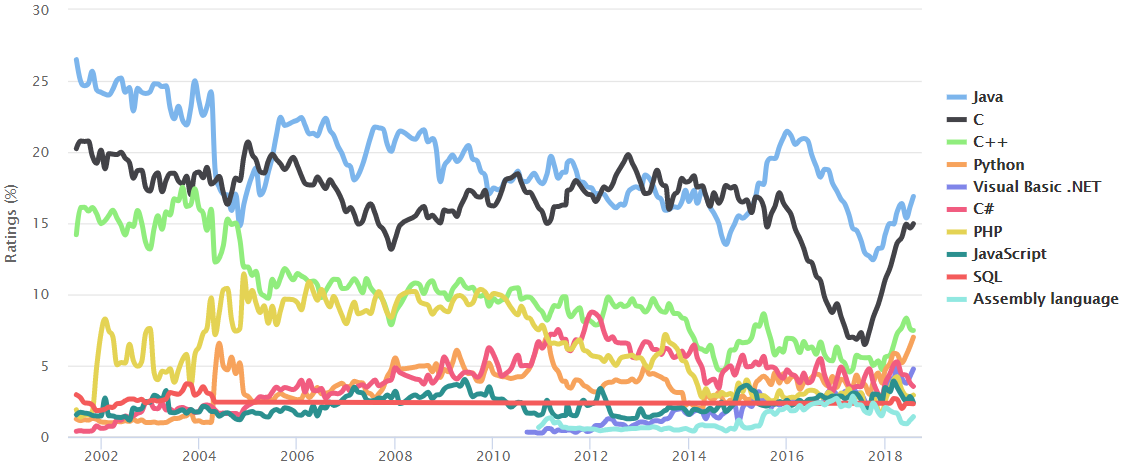
\includegraphics[scale=1.60]{Immagini/Capitolo1/TIOBEIndex}
\caption{TIOBE Programming Community Index (\href{www.tiobe.com}{www.tiobe.com})}
\label{fig:TIOBEIndex}
\end{figure}
%

%------------------------------ Software architecture -----------------------------
\section{Software architecture}
\label{sec1.2}

The following paragraphs deal with the organization of the code. In particular, the first paragraph describes how aircraft data is stored in XML files, while the second one focuses on the packages which constitutes \gls{JPAD}. There are currently six main packages and in the following chapters attention will be particularly focused on two of them: \lstinline[language=Java]!JPADCAD! and \lstinline[language=Java]!JPADCADSandbox!. The last section, instead, gives a brief overview on how and which kind of analyses are performed in \gls{JPAD}.

\subsection{Input files}
As previously mentioned, the input file type for \gls{JPAD} is the XML. In this way, aircraft data, operating conditions, and analyses requirements can be read by the software. XML stands for \emph{eXtensible Markup Language}. It is defined \emph{Markup Language} due to the use of tags that describe the content but, unlike other languages of the same type, the tags created in XML are self explanatory and the user is free to define his own tags, hence the \emph{eXtensible} definition. For this reason documents encoded using the XML format are both human-readable and machine-readable. XML support is provided by many programming languages (including Java) to create and process XML data. Simplicity, portability, platform independence, and usability are some of the key features that have resulted in the increasing popularity of the use of XML based standards. \cite{xmlWiki}

\bigskip
\noindent
More specifically, the XML file format can be summarized by the following concepts:
%
\begin{itemize}
\item tag,
\item attribute,
\item tree structure.
\end{itemize}
%
Each of the above mentioned points is reported in figure \ref{fig:xmlExample}: tags, which are contained between two brackets, are completely personalizable, can be completed by some attributes (such as units of measure) and can be innested, in order to obtain a convenient tree structure suitable for encoding typical data structures.
%
\begin{figure}[H]
\centering
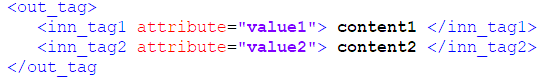
\includegraphics[scale=2.40]{Immagini/Capitolo1/xmlExample}
\caption{A simple XML example}
\label{fig:xmlExample}
\end{figure}
%

\bigskip
\noindent
In order to represent through the use of XML files the typical aircraft data structure, the input file setup designed by the Stanford University for their SUAVE project \cite{SUAVEProject} has been taken into account, deriving from it the folder tree represented in figure \ref{fig:JPADinputfoldertree}. As the figure shows, there's not just one input file storing all the data related to the aircraft. Instead, there's a XML file for each aircraft component and, as shown below, each component can call other XML files (e.g., lifting surfaces XMLs call for airfoil XMLs). The setup of a hierarchy among the XML files helps to reduce dramatically the dimension of each file and makes working with configuration files much easier, especially at high-level. In fact, the user can work fast and simply, assembling custom aircrafts through combination of chosen components XML files. An example of this capability is shown in listing \ref{lst:AircraftXML}, \ref{lst:HTailXML} and \ref{lst:AirfoilXML}. Figure \ref{fig:JPADinputfoldertree} also shows that a similar approach has been followed on the analysis side, splitting analysis XML in multiple files, each one dealing with a specific type of task (see also listing \ref{lst:AnalysesXML}).
%
\begin{figure}[H]
\centering
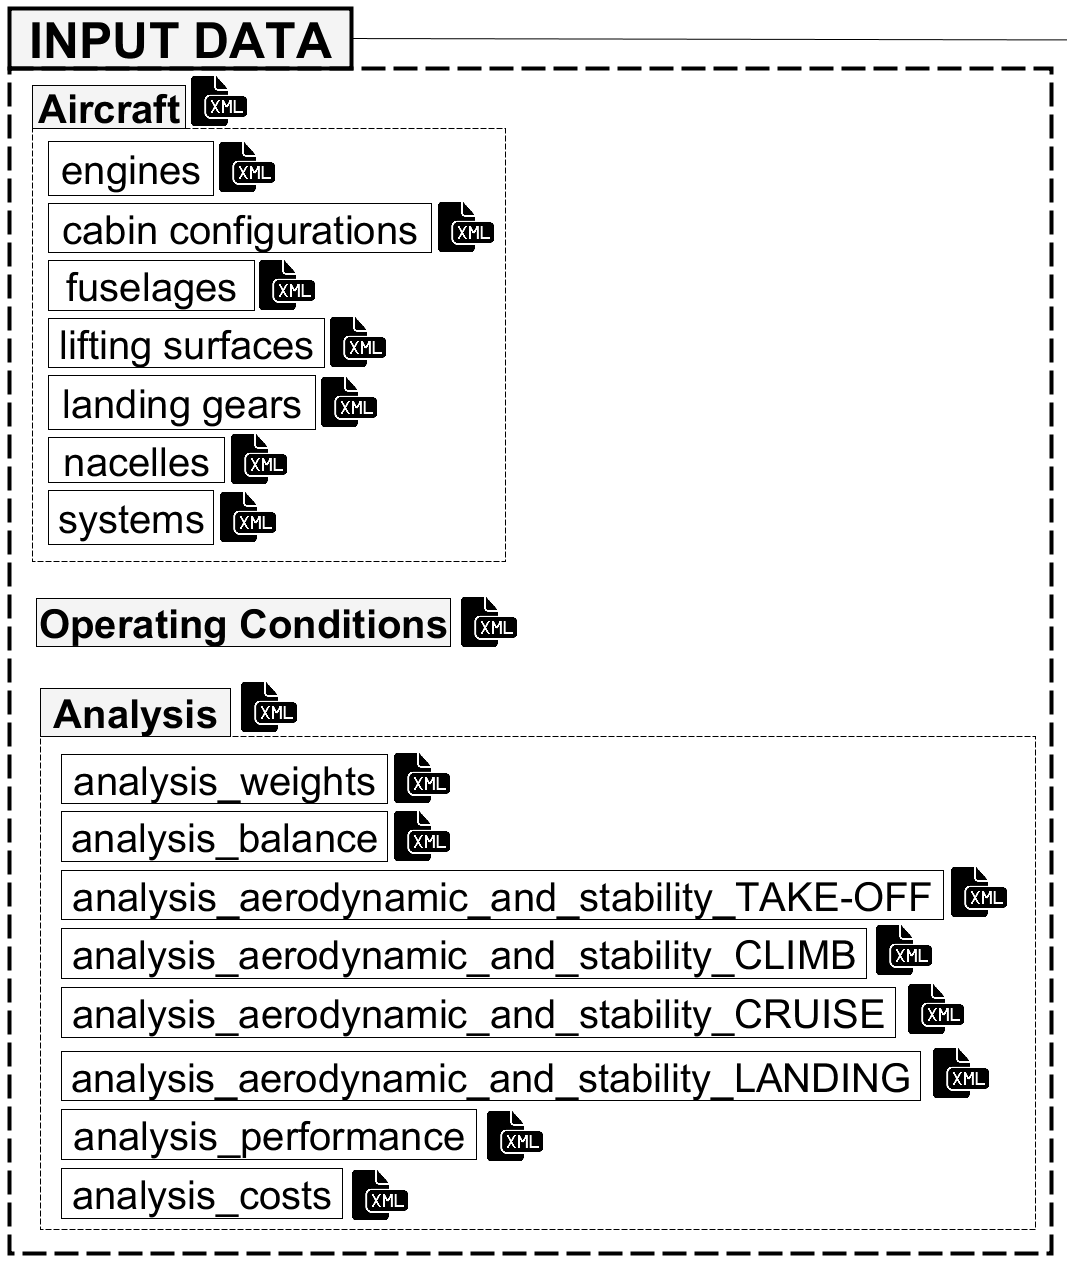
\includegraphics[scale=0.85]{Immagini/Capitolo1/JPADInputData}
\caption{JPAD input folder tree}
\label{fig:JPADinputfoldertree}
\end{figure}
%

\bigskip
\begin{lstlisting}[caption={Example of JPAD aircraft XML file}, captionpos=b, tabsize=6, language=XML, label={lst:AircraftXML}]
<jpad_config>
   <aircraft id="ATR-72" regulations="FAR_25" type="TURBOPROP">
      <lifting_surfaces>
         <wing file="wing_ATR72.xml">
            <position>
               <x unit="m">10.8</x>
               <y unit="m">0.0000</y>
               <z unit="m">1.6</z>
            </position>
            <rigging_angle unit="deg">3.0000</rigging_angle>
         </wing>
         <vertical_tail file="vtail_ATR72.xml">
            <position>
               <x unit="m">21.6</x>
               <y unit="m">0.0000</y>
               <z unit="m">1.3</z>
            </position>
            <rigging_angle unit="deg">0.0000</rigging_angle>
         </vertical_tail>
         <horizontal_tail file="htail_ATR72.xml">
            <position>
               <x unit="m">25.3</x>
               <y unit="m">0.0000</y>
               <z unit="m">5.7374</z>
            </position>
            <rigging_angle unit="deg">1.0000</rigging_angle>
         </horizontal_tail>
      </lifting_surfaces>
      <fuselages>
         <fuselage file="fuselage_ATR72.xml">
            <position>
               <x unit="m">0.0000</x>
               <y unit="m">0.0000</y>
               <z unit="m">0.0000</z>
            </position>
         </fuselage>
      </fuselages>
   </aircraft>
</jpad_config>
\end{lstlisting}

\bigskip
\begin{lstlisting}[caption={Example of JPAD lifting surface XML file}, captionpos=b, tabsize=6, language=XML, label={lst:HTailXML}]
<jpad_config>
   <horizontal_tail id="Horizontal tail" mirrored="true">
      <panels>
         <panel id="ATR72 horizontal tail">
            <span unit="m">3.6548</span>
            <dihedral unit="deg">0.0000</dihedral>
            <sweep_leading_edge unit="deg">13.4400</sweep_leading_edge>
            <inner_section>
               <chord unit="m">2.0440</chord>
               <airfoil file="naca0012.xml"/>
               <geometric_twist>0.000000</geometric_twist>
            </inner_section>
            <outer_section>
               <chord unit="m">1.1652</chord>
               <airfoil file="naca0012.xml"/>
               <geometric_twist unit="deg">0.0000</geometric_twist>
            </outer_section>
         </panel>
      </panels>
      <symmetric_flaps>
         <symmetric_flap id="Elevator" type="PLAIN">
            <inner_station_spanwise_position>0.1</inner_station_spanwise_position>
            <outer_station_spanwise_position>0.9</outer_station_spanwise_position>
            <inner_chord_ratio>0.3000</inner_chord_ratio>
            <outer_chord_ratio>0.3000</outer_chord_ratio>
            <min_deflection unit="deg">-25.0</min_deflection>
            <max_deflection unit="deg">5.0</max_deflection>
         </symmetric_flap>
      </symmetric_flaps>
   </horizontal_tail>
</jpad_config>
\end{lstlisting}

\bigskip
\begin{lstlisting}[caption={Example of JPAD airfoil XML file}, captionpos=b, tabsize=2, language=XML, label={lst:AirfoilXML}]
<jpad_config>
    <airfoil family="NACA_4_Digit" name="NACA0012" type="CONVENTIONAL">
        <geometry>
            <thickness_to_chord_ratio_max>0.1200</thickness_to_chord_ratio_max>
            <radius_leading_edge_norm unit="m">0.0158</radius_leading_edge_norm>
            <x_coordinates>[...]</x_coordinates>
            <z_coordinates>[...]</z_coordinates>
        </geometry>
        <aerodynamics>
            <alpha_zero_lift unit="deg">0.0000</alpha_zero_lift>
            <alpha_end_linear_trait unit="deg">11.0000</alpha_end_linear_trait>
            <alpha_stall unit="deg">20.1000</alpha_stall>
            <Cl_alpha_linear_trait unit="1/rad">6.9200</Cl_alpha_linear_trait>
            <Cl_at_alpha_zero>0.000000</Cl_at_alpha_zero>
            <Cl_end_linear_trait>1.2300</Cl_end_linear_trait>
            <Cl_max>1.8600</Cl_max>
            <Cd_min>0.005500</Cd_min>
            <Cl_at_Cdmin>0.000000</Cl_at_Cdmin>
            <laminar_bucket_semi_extension>0.000000</laminar_bucket_semi_extension>
            <laminar_bucket_depth>0.000000</laminar_bucket_depth>
            <K_factor_drag_polar>0.003500</K_factor_drag_polar>
            <Cm_alpha_quarter_chord unit="1/deg">0.0000</Cm_alpha_quarter_chord>
            <Cm_ac>0.000000</Cm_ac>
            <Cm_ac_at_stall>-0.090000</Cm_ac_at_stall>
            <x_ac_normalized>0.2500</x_ac_normalized>
            <mach_critical>0.7340</mach_critical>
            <x_transition_upper>0.1200</x_transition_upper>
            <x_transition_lower>0.1200</x_transition_lower>
        </aerodynamics>
    </airfoil>
</jpad_config>
\end{lstlisting}

\subsection{Libraries}
\gls{JPAD} is currently made of six main packages, each one of them dealing with specific tasks. Moreover, each package can contain several sub-packages (organized in classes and utilities) pertinent to more specialized assignments. This kind of organization, called modularity, helps in terms of code mainteinance: part of the system can be updated in case of issues without a need to make large-scale changes. Besides, modularity makes working with the code much easier in an ever changing team.

\bigskip
\noindent
The six packages that constitutes \gls{JPAD} are: \lstinline[language=Java]!JPADCore! (actually, \lstinline[language=Java]!JPADCore_v2! due to the intense changes occurred during the last months), \lstinline[language=Java]!JPADConfigs!, \lstinline[language=Java]!JPADCommander!, \lstinline[language=Java]!JPADCAD!, \lstinline[language=Java]!JPADSandBox! (actually, \lstinline[language=Java]!JPADSandBox_v2!), and \lstinline[language=Java]!JPADCADSandBox!. The next sections describe each package individually, summarizing the characteristics and the tasks of each one of them.

\subsubsection{\texttt{JPADCore}}
\lstinline[language=Java]!JPADCore!, as the name suggests, is \gls{JPAD} main package. It currently contains the following sub-packages.
%
\begin{itemize}
\item \lstinline[language=Java]!aircraft!, which contains sub-packages dedicated to aircraft components (fuselage, lifting surfaces, nacelles, power plant, cabin configuration) and classes managing landing gears and systems mounted on board. As previously mentioned for the input XML structure side, the lifting surfaces package also contains the classes managing the airfoils.
\item \lstinline[language=Java]!analyses!, which contains the managers for five types of analysis that can be performed on aircrafts: weights, balance, aerodynamics and stability, performance, and costs. Additionally, \lstinline[language=Java]!analyses! also contains sub-packages (one for each of the before mentioned aircraft components) enclosing component's manager classes for weigths, balance and aerodynamic calculation. Finally, classes managing the operating conditions are stored in this package too.
\item \lstinline[language=Java]!calculators!, actually containing all the methods and the formulas needed to perform all the previously mentioned analyses.
\item \lstinline[language=Java]!database!, containing the classes used in order to read data from HDF files (reader can refer to \cite{HDFWiki} for more information about). In particular, these classes manage the data reading process from aerodynamics and engine databases.
\item \lstinline[language=Java]!standaloneutils!, which encloses several utility classes, i.e., classes containing methods that can be accessed in a static way. These utilities cover the most various needings, from Standard Atmoshere properties calculation to XML file reading.
\item \lstinline[language=Java]!writers!, finally, enclosing classes useful in order to store results.
\end{itemize}
%

\subsubsection{\texttt{JPADConfigs}}
\lstinline[language=Java]!JPADConfigs! is the package containing all the enumeration classes used in \gls{JPAD}. In computer programming, enumerations consist of a set of named values. The enumerator names are usually identifiers that behave as constants in the language. In the Java programming language, enumeration types are defined using the \lstinline[language=Java]!enum! keyword; because values assumed by enumeration type variables are constant, the names of an \lstinline[language=Java]!enum! type fields are in uppercase letters. \cite{JavaEnum}

\bigskip
\noindent
Like the \lstinline[language=Java]!standaloneutils! classes, enumerations contained in \lstinline[language=Java]!JPADConfigs! cover very different fields: some such as \lstinline[language=Java]!ComponentEnum! and \lstinline[language=Java]!AirplaneType! regard the aircraft and its characteristics, while others, such as \lstinline[language=Java]!MethodEnum! and \lstinline[language=Java]!AnalysisTypeEnum!, deal with the analyses.

\subsubsection{\texttt{JPADCommander}}
\lstinline[language=Java]!JPADCommander! contains the classes which allow the \gls{JPAD} \gls{acr:GUI} (simply called JPADCommander in the rest of the paragraph) to work. 

\bigskip
\noindent
\gls{JPAD} comes with a simple yet very intuitive \gls{acr:GUI}. In order to simplify the management of all the operations required for the definition of the aircraft parametric model and its analysis, JPADCommander guides the user through a path which starts with the definition of the working folders and ends with the management and visualization of the output. In particular, JPADCommander interfaces with the user by means of four main windows. The first one is a configuration window, through which the user defines:
%
\begin{itemize}
\item working directory,
\item input directory,
\item output directory,
\item database directory.
\end{itemize}
%
The second screen gives the user the possibiity to choose between \emph{Input}, \emph{Analysis} and \emph{Results}. As soon as the user has defined the previously mentioned folders, the only option available is the one regarding the input, with the analysis button becoming available just after the input phase has been performed. The same happens for the results button, which becomes clickable after the user has performed the analysis phase. The third screen, the one regarding the Input Manager, is shown in figure \ref{fig:GUIInputManager}. Here, the user has three possibilities:
%
\begin{itemize}
\item loading a default aircraft,
\item importing aircraft data from file,
\item generating a new aircraft filling in all the fields in the Input Manager screen.
\end{itemize}
%
Figure \ref{fig:GUIInputManager} also shows that the Input Manager screen has several additional pages, dedicated to each of the aircraft components mentioned in the input file section. After completing the input phase, clicking the \emph{Home} button the user will have access to the Analysis Manager screen, which is shown in figure \ref{fig:GUIAnalysisManager}. In this module, the user can define which analyses he wants to perform. As for the Input Manager, also in this case the user has the possibility to load a previously saved analysis or fill in the available fields. Finally, as soon as the analyses have been performed, results become available from the main screen.
%
\begin{figure}[H]
\centering
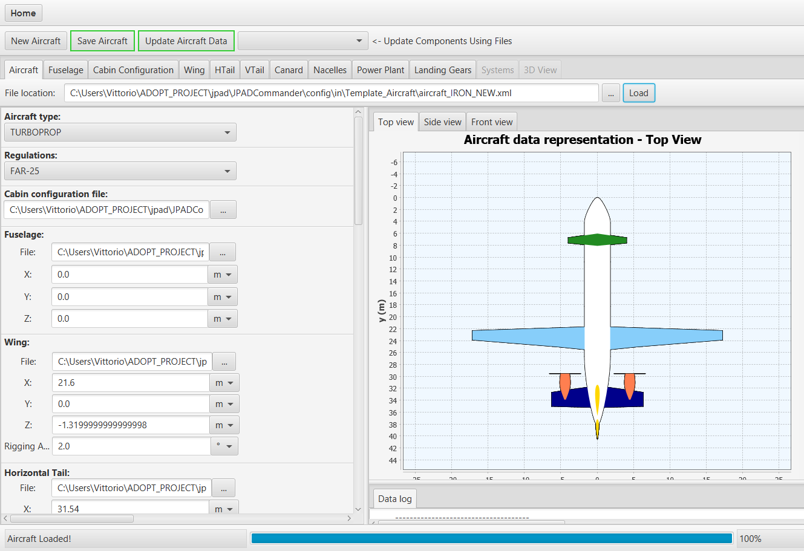
\includegraphics[scale=2.0]{Immagini/Capitolo1/AircraftInputManager}
\caption{JPADCommander Aircraft Input Manager screen}
\label{fig:GUIInputManager}
\end{figure}
%
\begin{figure}[H]
\centering
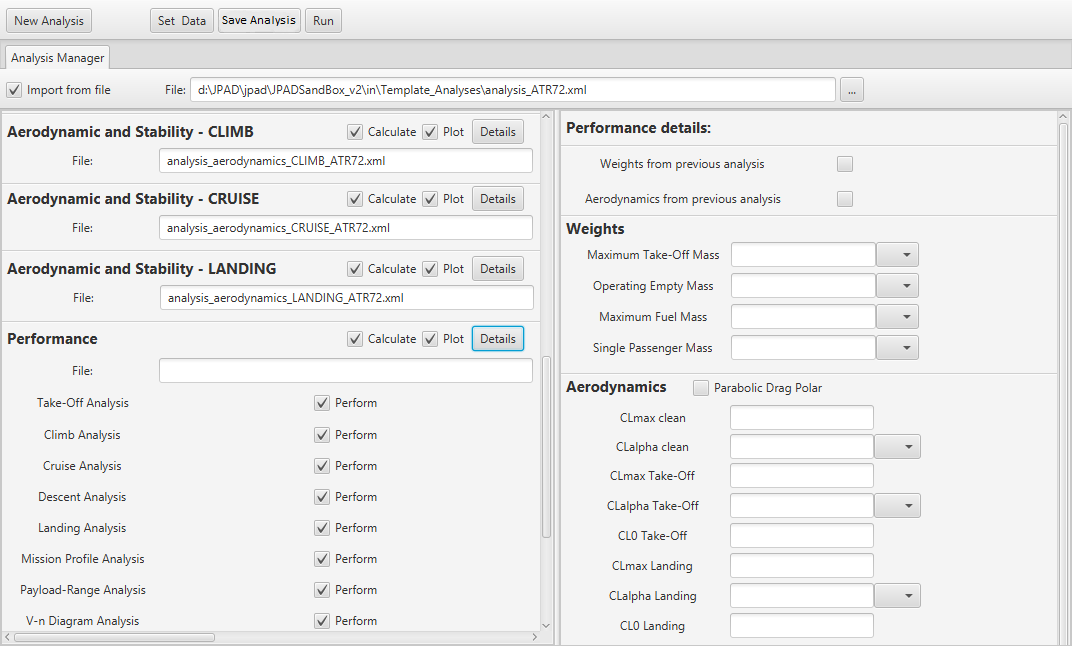
\includegraphics[scale=1.5]{Immagini/Capitolo1/AnalysisManagerGUI}
\caption{JPADCommander Analysis Manager screen}
\label{fig:GUIAnalysisManager}
\end{figure}
%

\subsubsection{\texttt{JPADSandBox}}
This package contains all the test classes, i.e., classes (mostly containing main methods) used in order to test new methods or functionalities, before adding them to \gls{JPAD} main libraries. It encloses several packages, one for each developer, in which individual tests can be written and performed. Besides, it also contains the folders in which template aircraft and analysis XMLs are stored.

\subsubsection{\texttt{JPADCAD} - \texttt{JPADCADSandBox}}
Generating \gls{CAD} models can be an important achievement for a software such as \gls{JPAD} for several reasons.
%
\begin{itemize}
\item It gives an immediate feedback about the data provided to the application: in case of mistakes, the \gls{CAD} model helps detecting them almost immediately.
\item It allows the user to run a \gls{CFD} analysis using an external tool. In fact, \gls{JPAD} generated \gls{CAD} models are ready to be meshed without any further adjustment.
\item It provides an accurate estimate of the wet surface of each component.
\end{itemize}
%
\lstinline[language=Java]!JPADCAD! and \lstinline[language=Java]!JPADCADSandbox! are the packages which currently contain all the classes and utility classes necessary to the creation of geometric and topological entities. Shapes (i.e., basic topological entities) can be exported into various file formats (e.g., STEP or IGES) and opened in any desired \gls{CAD} software. Generating the most various shapes is made possible by the use of the \gls{OCCT} classes, which are actually written in C++, but can be used in \gls{JPAD} thanks to the \gls{OCCT} Java Wrapper, a tool which allows the use of \gls{OCCT} classes from within Java applications. The static methods which actually perform the translation from the aircraft geometric data (stored, as previously mentioned, in the XML file format) to CAD file format currently reside in \lstinline[language=Java]!AircraftUtils!, a \lstinline[language=Java]!JPADCADSandbox! utility class. The same package also contains all the tests performed for this thesis work.

\subsection{Analyses}
\label{sec1.3}

The main purpose of \gls{JPAD} is to perform different analyses and to provide the data necessary for the comparison of different aircraft or different configurations of the same aircraft. The previously described XML structure easily allows this. Besides, the same hierarchical structure has been replicated for the analyses, as reported in listing \ref{lst:AnalysesXML}, giving the user the possibility to perform a complete analysis (i.e., executing all the analyses contained in \lstinline[language=Java]!JPADCore!), or specific ones, combining different analysis files. This allows an easier evaluation of a generic cost function during optimization tasks, resulting in a reduced amount of computational costs required for this kind of operations.

\bigskip
\begin{lstlisting}[caption={JPAD analyses XML file, not needed analyses are commented}, captionpos=b, tabsize=6, language=XML, label={lst:AnalysesXML}]
<jpad_config>
    <!-- Input data, shared across analysis tasks -->
    <global_data>
        <positive_limit_load_factor>2.5</positive_limit_load_factor>
		<negative_limit_load_factor>-1.0</negative_limit_load_factor>
    </global_data>
    <!-- Required analysis tasks - comment the tag of the analysis if not needed -->
    <analyses id="ATR-72 analysis" iterative_loop="FALSE">
		<weights 
            file="analysis_weights_ATR72.xml" 
			plot="TRUE"
			create_CSV="TRUE"
            method_fuselage=""
            method_wing=""
            method_htail=""
            method_vtail=""
			method_canard=""
			method_nacelles=""
			method_power_plant=""
			method_landing_gears=""
			method_APU=""
			method_air_conditioning_and_anti_icing=""
			method_instruments_and_navigation_system=""
			method_hydraulic_and_pneumatic_systems=""			
			method_electrical_systems=""
			method_furnishings_and_equipments=""
			method_control_surfaces=""
            />
		<balance 
			file="analysis_balance_ATR72.xml"
			plot="TRUE"
			create_CSV="TRUE"
            method_fuselage=""
            method_wing=""
            method_htail=""
            method_vtail=""
			method_canard=""
			method_nacelles=""
			method_power_plant=""
			method_landing_gears=""
		/>
		<!--
		<aerodynamic_and_stability
			plot="FALSE"
			create_CSV="FALSE"
			take_off_condition="TRUE"
			file_take_off_condition="analysis_aerodynamics_ATR72_takeoff.xml"
			climb_condition="TRUE"
			file_climb_condition="analysis_aerodynamics_ATR72_climb.xml"
			cruise_condition="TRUE"
			file_cruise_condition="analysis_aerodynamics_ATR72_cruise.xml"
			landing_condition="TRUE"
			file_landing_condition="analysis_aerodynamics_ATR72_landing.xml"
		/>
		<performance 
			file="analysis_performance_ATR72.xml"
			plot="FALSE"
			create_CSV="FALSE"
			take_off="FALSE"
			climb="FALSE"
			cruise="FALSE"
			descent="FALSE"
			landing="FALSE"
			payload_range="FALSE"
			V_n_diagram="FALSE"
			mission_profile="TRUE"
		/>
		<costs 
			file="analysis_costs_ATR72.xml"
			plot="FALSE"
			create_CSV="FALSE"
			doc_capital="TRUE"
			doc_capital_method="AEA"
			doc_crew="TRUE"
			doc_crew_method="AEA"
			doc_fuel="TRUE"
			doc_fuel_method="AEA"
			doc_charges="TRUE"
			doc_charges_method="ILR_AACHEN"
			doc_maintenance="TRUE"
			doc_maintenance_method="ATA"
		/> 
		-->
    </analyses>
</jpad_config>
\end{lstlisting}

\bigskip
\noindent
\gls{JPAD} currently allows five types of analysis.
%
\begin{itemize}
\item Weights analysis: estimates the aircraft weight breakdown starting from a first guess maximum take-off weight and specific mission requirements. In particular, it evaluates each aircraft component mass using well-known semi-empirical methods.
\item Balance analysis: estimates the centre of gravity position related to each weight condition and draws the balance diagram.
\item Aerodynamics and Stability analysis: the aerodynamics module estimates all the aerodynamic characteristics in terms of lift, drag and moment coefficients, at different operating conditons and for each aircraft component (wing, tails, fuselage, and nacelles); whereas the stability module reports data concerning the aircraft static stability.
\item Performance analysis: evaluates aircraft most important performances, such as payload-range diagram, mission profile, cruise flight envelope, ground performance, climb performance, and cruise grid chart.
\item Costs analysis: estimates the \gls{DOC} breakdown.
\end{itemize}
%
In addition to multidisciplinary analyses, \gls{JPAD} is also able to perform parametric studies and \gls{MDO}. In both cases it is possible to define a set of parameters to be varied, typically geometric, and the input manager will provide for the generation of all the test aircrafts thanks to the combination of different files for the individual components. Once all the required configurations are ready, it will be possible to choose whether to carry out a parametric study or an optimization. It will be necessary to define one or more objectives to be monitored and one or more constraints to be respected; the latter can be selected from a dedicated list. Once all the parameters have been defined, \gls{JPAD} will launch all the analyses necessary for the evaluation of the objectives and the required constraints, with the possibility of exploiting serial or parallel analyses (i.e., executed on more threads) in order to reduce calculation times. Once all the required calculation have been completed, one or more response surfaces will be obtained which, on the one hand, constitute the output of the parametric study, while on the other they can be used as input for optimization (figure \ref{fig:JPADParametricStudy}). 
%
\begin{figure}[htbp]
\centering
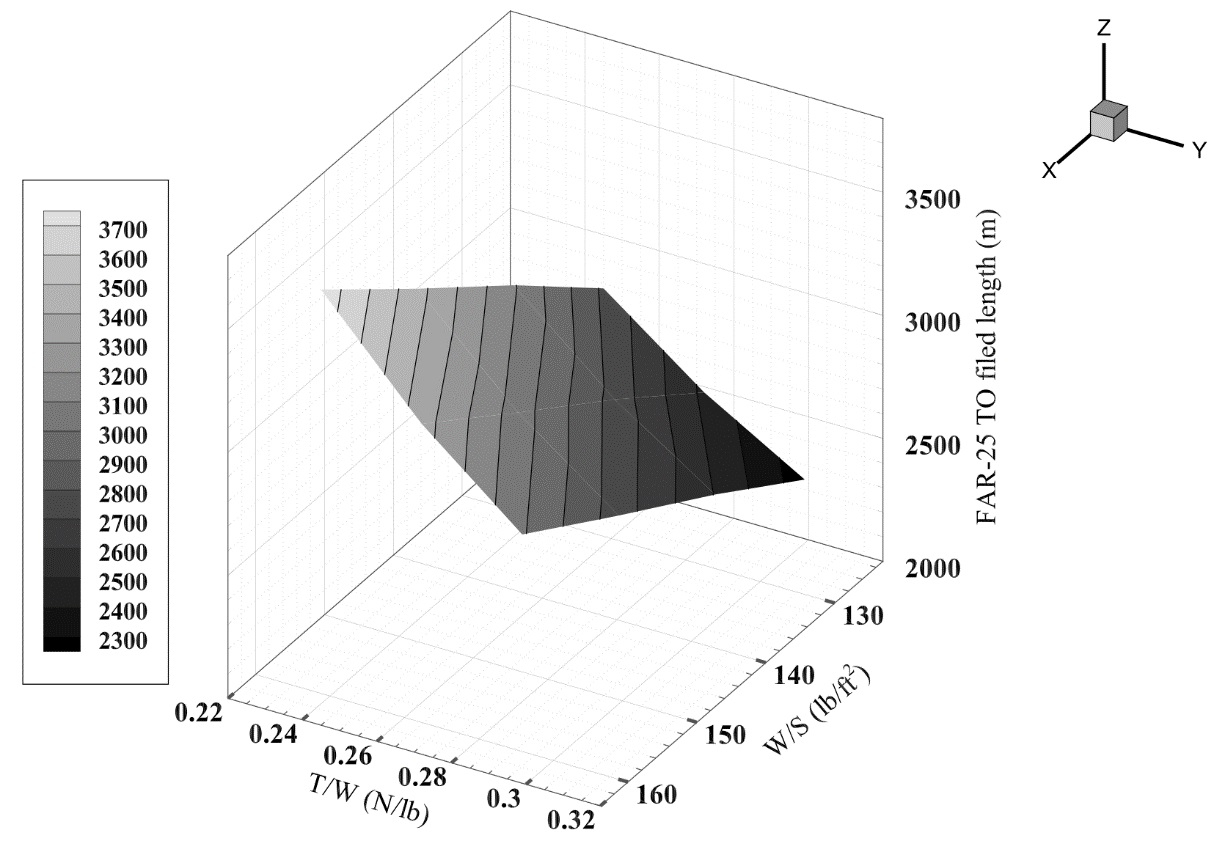
\includegraphics[height=0.27\textheight]{Immagini/Capitolo1/JPADParametricStudy}
\caption{Example of parametric study performed in JPAD on a Boeing B747-100B}
\label{fig:JPADParametricStudy}
\end{figure}
%

\bigskip
\noindent
Figure \ref{fig:JPADFlowchart} shows JPAD typical flowchart, summarizing the concepts expressed in the previous paragraphs. In particular, it clearly makes a distinction between the input (aircraft and analysis data) and the core (the analysis itself).
%
\begin{figure}[htbp]
\centering
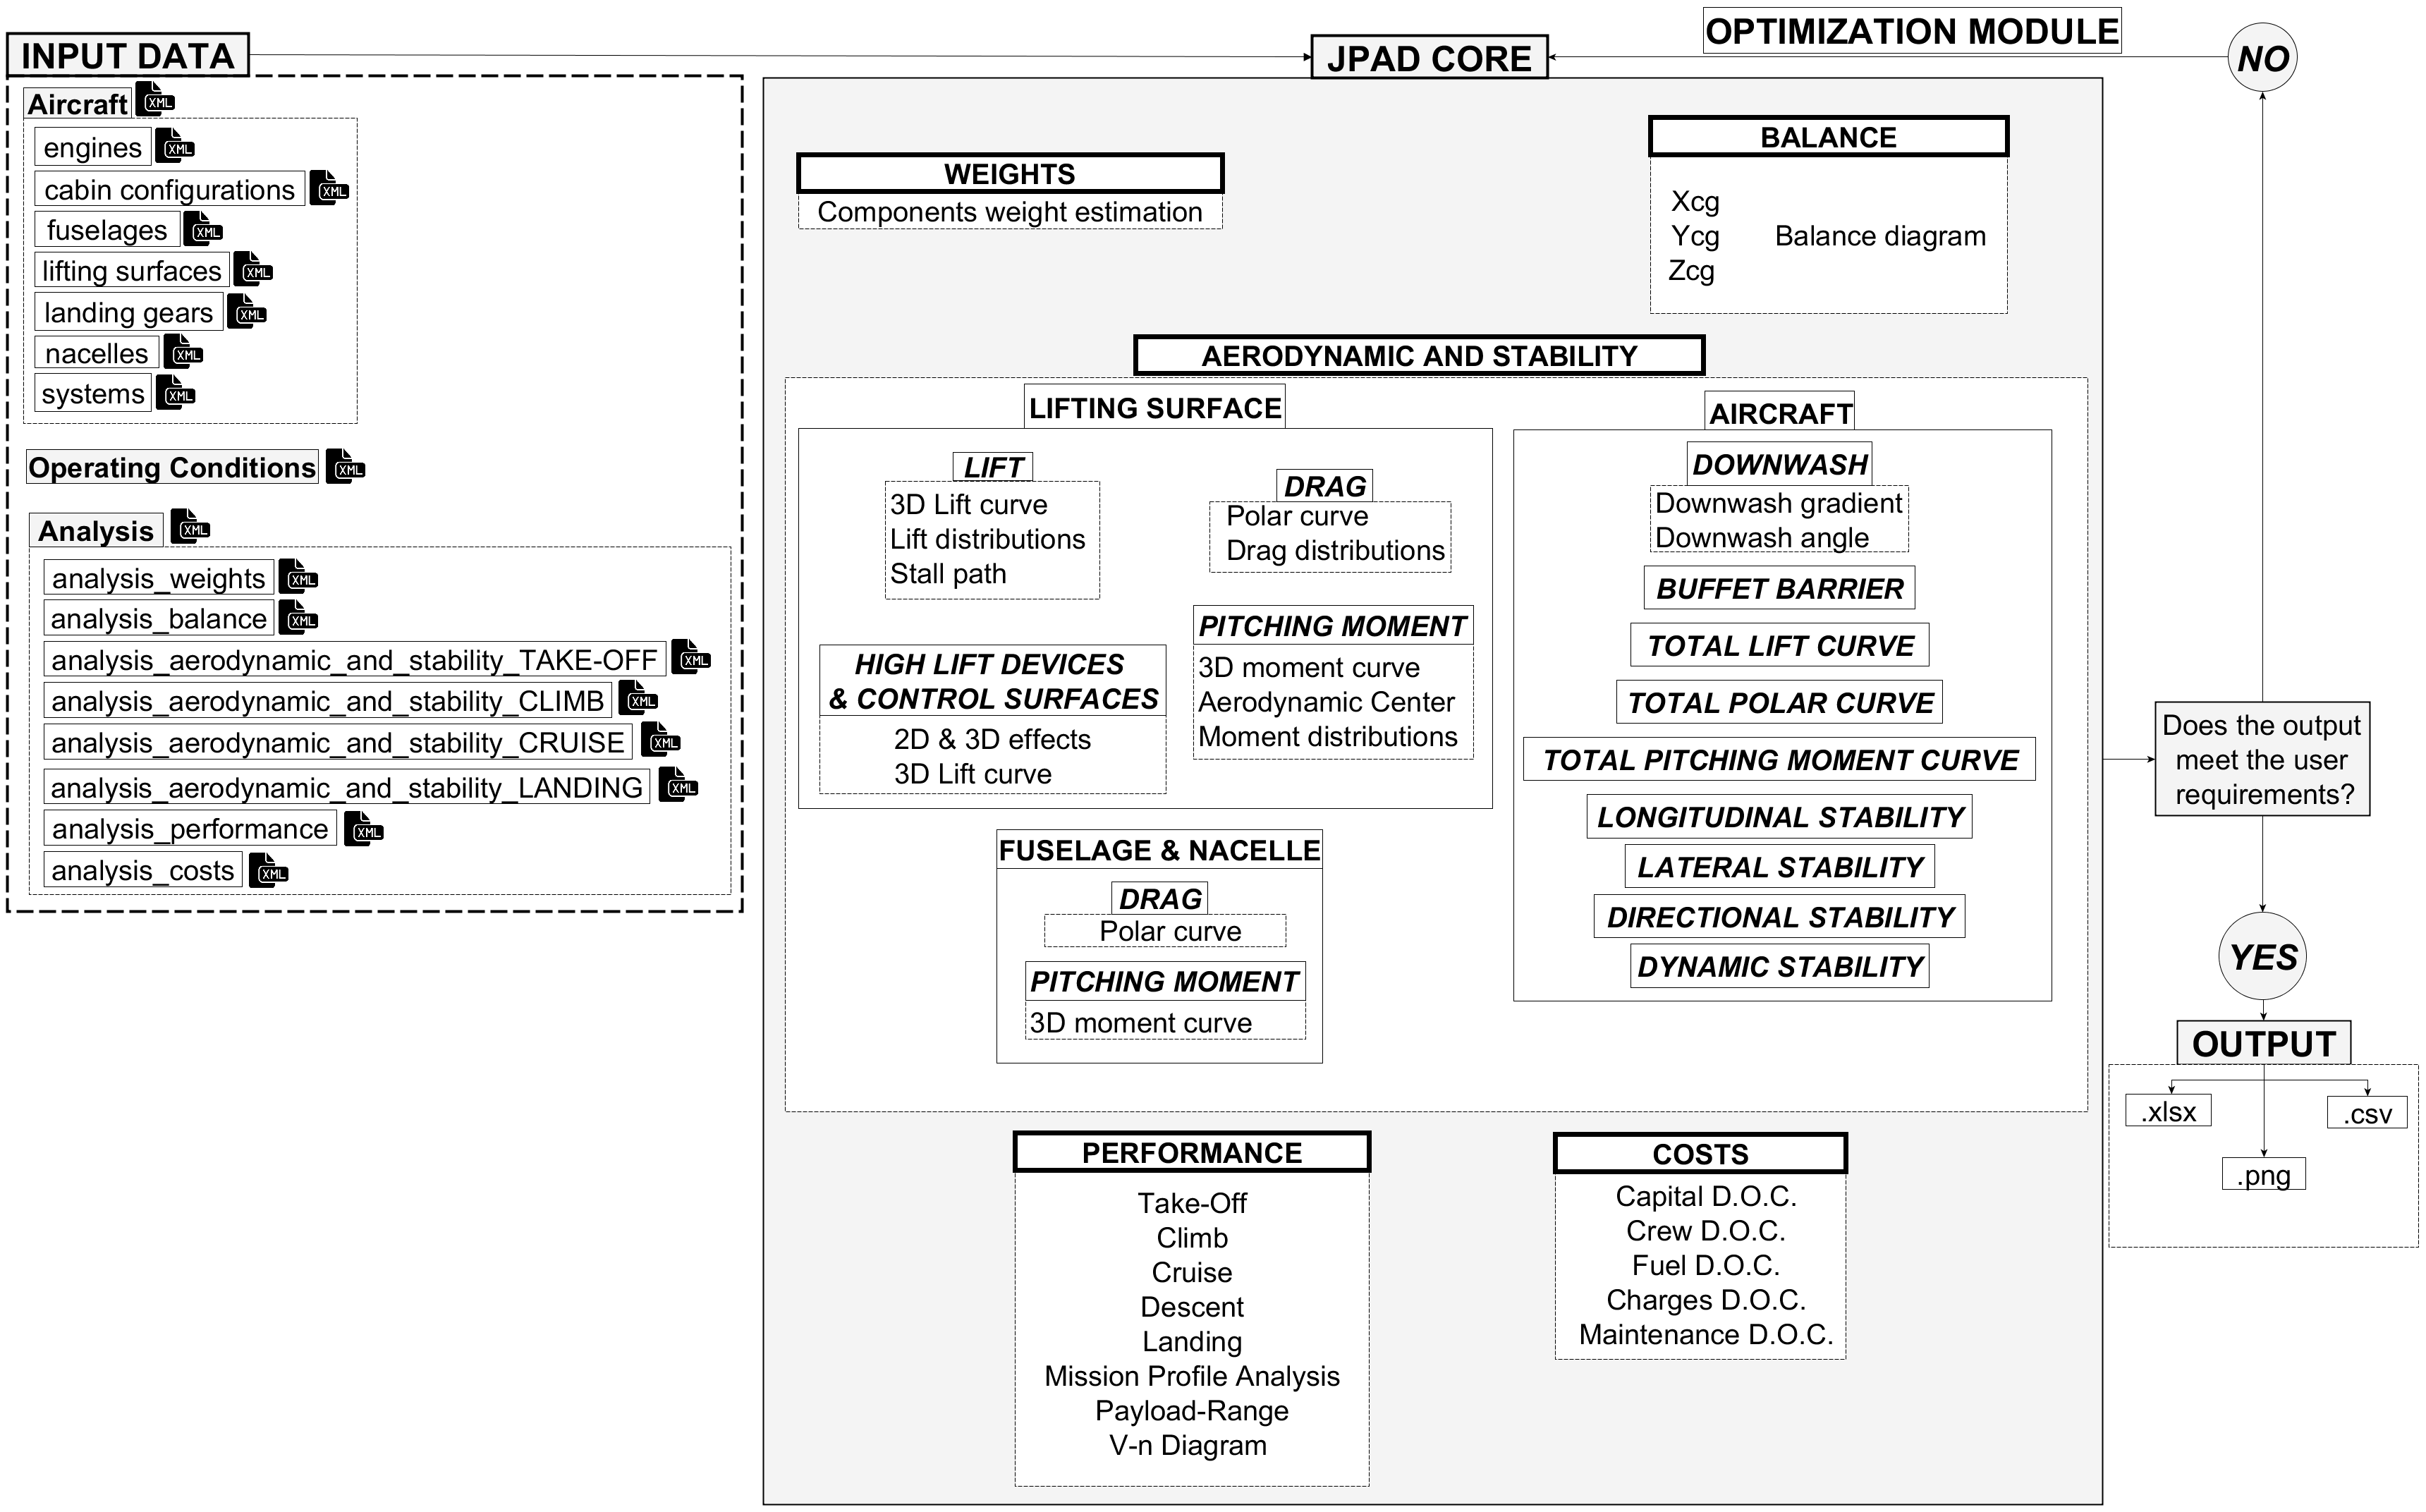
\includegraphics[height=0.36\textheight]{Immagini/Capitolo1/JPADFlowchart}
\caption{JPAD flowchart}
\label{fig:JPADFlowchart}
\end{figure}
%


%------------------------------- JPADCAD module --------------------------------
\chapter{\texttt{JPADCAD} module}
\label{chap2}

%------------------------------- CAD: motivations and approaches --------------------------------
\section{CAD: motivations and approaches}
\label{sec2.1}

In paragraph \ref{sec1.2}, it was mentioned why the generation of a 3D \gls{CAD} model in a software such as \gls{JPAD} could prove particularly useful. In this section the attention will be focused even more on the motivations that may lead to the need to generate a complete 3D model of the aircraft even in the initial design stages. 

\bigskip
\noindent
\gls{CFD} has increasingly become, over the last three decades, an indispensable tool for aerodynamic studies in aircraft design. Nowadays, viscous \gls{CFD} simulations are carried out in ever increasing numbers and at all stages of the design. \gls{CFD} is particularly useful in terminal project stages, when simulations are required in the most disparate phases of flight (such as take-off or landing). With the possibility of producing unstructured mesh, the spectrum of \gls{CFD} applications has expanded further, and, at the moment, there seem to be no limits to the geometric complexity that can be fed to \gls{CFD} solvers. This also happens thanks to the continouos reduction of the time needed to create the mesh and perform the calculations. Engineers can now perform complex simulations using a simple desktop computer, when, on the other hand, the same simulations would have required a cluster for parallel computing only a few years ago. This growing computing power has given engineers the ability to carry out most of the design and analysis work of complex systems without the need to resort to physical models or prototypes.

\bigskip
\noindent
Nowadays there is an ever increasing demand in the aerospace industry to use \gls{CFD} analysis even in the preliminary and conceptual phases of aircraft design. This is due to the fact that \gls{CFD} simulations can predict the compressible and viscous flow fields around the aircraft taking into account all the important aerodynamic phenomena. The result is the achievement of forces on points on the surfaces or integral forces for each of the components of the aircraft. These forces will take into account viscous and transonic phenomena and interferences between components, with a reliable accuracy. Moreover, in the cases in which it is desired to analyze new and uncommon configurations, the estimation of certain aerodynamic characteristics through the traditional techniques of the preliminary design phase could be difficult or completely impossible. This is because many of these methods, of an empirical or semiempirical nature, have been conceived and calibrated for use in the case of classical or ordinary configurations. In this case, the \gls{CFD} analysis would come to the rescue, limiting the risks of making gross errors in the early design phases. \cite{paperCADinAero} 

\bigskip
\noindent
But aerodynamics is not the only domain that needs to be investigated. In a multi-disciplinary design context, such as that of aircraft design, engineers have to deal with different disciplines at the same time, and necessitate to make sure the solutions they come up to are the closest possible to the optimum ones. Traditionally, in the early stages of design, engineers are in possess of what is defined as the \gls{acr:OML} of the aircraft, and the details of other subsystems, such as structural layouts, are not examined until later design phases. But, in general, the configuration's \gls{acr:OML} geometry design is impacted by these subsystems, and it may be not discovered until high-fidelity analyses are performed in later development phases. Besides, further complications could arise whenever the geometry definition is scattered over many different analysis methods, which can span different disciplines as well as different fidelity levels within a discipline. What could happen is that geometry adjustments from redesign based on one method are likely to be inconsistent with the other geometry definitions. One solution to these difficulties and complications is, again, to generate a 3D model of the aircraft much earlier during the design study, as during the preliminary or even the conceptual phase, and to use this 3D model for all the possible analyses. Having a 3D model at disposal during conceptual design phase and performing on it higher fidelity analyses (alongside low-fidelity ones) would lead to a greater confidence in calculated data and for configuration down-select. Besides, there would be no need to generate new and more precise geometries as the design process progresses, because the 3D model of the aircraft would mature during the design process itself. \cite{AIAApaperHaimesDrela}

\bigskip
\noindent
What appears quite clear from the previous examination is that the performing of high-fidelity analyses is something really auspicable even during the first stages of the aircraft design process. But, in order to perform these analyses, an adequate geometry generator must be used. At this stage several approaches can be considered, especially when parametrization and \gls{MDO} need to be taken into account. 

\bigskip
\noindent
A \gls{acr:FFD} volume approach for \gls{CAD}-free geometry parametrization can be followed, as presented in \cite{AIAApaperKenwayKennedy}. The \gls{acr:FFD} approach is borrowed directly from soft object animation in the computer graphics field and allows to perform high level modifications to complex objects by simply embedding them in a rubber-like volume, which is stretched and twisted in order to obtain, indirectly, the desired final shape for the object (figure \ref{fig:FFD}). One key observation that needs to be made about \gls{acr:FFD} is that it parametrizes not the geometry itself, but the geometry change. This brings to an efficient computation of analytic derivatives for gradient-based optimization.
%
\begin{figure}[H]
\centering
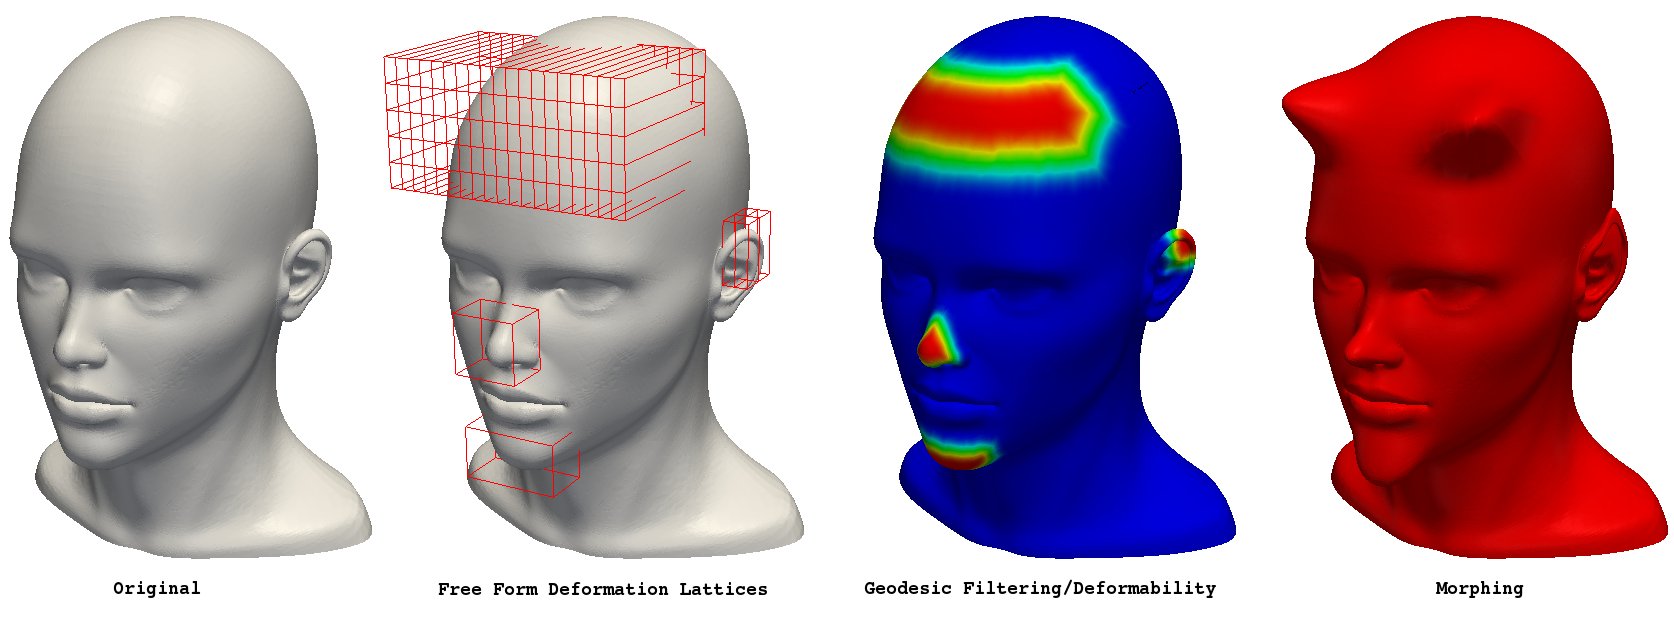
\includegraphics[scale=1.05]{Immagini/Capitolo2/ffdprocedure}
\caption{Free-form deformation example (\href{www.optimad.it/wp-content/uploads/ffdprocedure.png}{www.optimad.it/wp-content/uploads/ffdprocedure.png})}
\label{fig:FFD}
\end{figure}
%

\bigskip
\noindent
A further approach to the problem is described in \cite{paperCADinAero}, in which the author examines the potential of parametric \gls{CAD} systems and the help they can offer during the early stages of aircraft design. In a parametric CAD software, contrary to what happens in conventional \gls{CAD} systems, at each step the user has the possibility to name the entity that is being created and to make a parameter one or more values of the entity itself. In the event that one of the parameters is changed, all the child entities of the element to which the mutated parameter belongs are updated.

\bigskip
\noindent
One last possible approach is the one used in \cite{AIAApaperHaimesDrela}, which involves the generation of a general geometry \gls{acr:API} in order to create solids-based geometries. In particular, the \gls{acr:API} created by the authors (named EGADS) provides a solid modeling geometry kernel that supports both \emph{Bottom-Up} construction (i.e., the process of producing a solid model from its constituent geometric entities) as well as the ability to perform \gls{CSG} operations. Both capabilities are necessary in order to build closed 3D models, which are essentials for high-fidelity analyses. The core of EGADS is Open CASCADE, a fully functional open-source solid modeling geometry kernel, which incorporates all the methods and operations necessary to perform shape manipulation. Since the approach is \emph{Bottom-Up} and programmatic (each of the geometric and topological entities is assigned one or more manageable variables) the 3D \gls{CAD} models produced will be, to a certain extent, parametrized \emph{a priori}. As it will be more clear from the following paragraphs, the approach used for \gls{JPAD} is pretty similar to the latter.

%------------------------------- Open CASCADE Technology --------------------------------
\section{Open CASCADE Technology}
\label{sec2.2}

As anticipated in section \ref{sec2.1}, the \lstinline[language=Java]!JPADCAD! module helps the user to build from scratch, in a \emph{Bottom-Up} approach, aircraft solid components ready to be passed to a \gls{CFD} solver, in order to perform high-fidelity analysis. This would have not been possible without the adoption of an external library such as \gls{OCCT}.

\bigskip
\noindent
Open CASCADE Technology (\gls{OCCT}) is an object-oriented C++ class library designed for rapid production of sophisticated domain-specific \gls{CAD} applications. A typical application developed using \gls{OCCT} deals with 2/3D geometric modeling in general-purpose or specialized \gls{CAD} systems, manifacturing or analysis applications, simulations applications, or even illustration tools. \gls{OCCT} provides classes for several purposes, such as:
%
\begin{itemize}
\item basic data structures (e.g., geometric modeling, visualization, interactive selection);
\item modeling algorithms;
\item working with mesh;
\item data interoperability with neutral formats, such as IGES and STEP.
\end{itemize}
%
The C++ classes are located into packages, which are organized into toolkits, which are finally grouped into seven modules \cite{webOpenCASCADE} (figure \ref{fig:OCCTStructure}):
%
\begin{itemize}
\renewcommand\labelitemi{\tiny$\blacksquare$}
\item \textbf{Foundation Classes} module underlies all other \gls{OCCT} classes;
\item \textbf{Modeling Data} module supplies data structures to represent 2D and 3D geometric primitives and their compositions into \gls{CAD} models;
\item \textbf{Modeling Algorithms} module contains a wide range of geometrical and topological algorithms;
\item \textbf{Mesh} module implements tessellated representation of objects;
\item \textbf{Visualization} module provides mechanisms for graphical data representation;
\item \textbf{Data Exchange} module interacts with popular data formats and relies on \textbf{Shape Healing} module to improve compatibility between different \gls{CAD} software;
\item \textbf{Application Framework} module offers solutions for handling application-specific data and commonly used functionality (e.g., save/restore, undo/redo, copy/paste).
\end{itemize}
%
In addition, Open CASCADE comes equipped with a convenient testing tool, called \textbf{Test Harness} or \textbf{Draw}, that can be used to test and prototype various algorithms before building an entire application.
%
\begin{figure}[H]
\centering
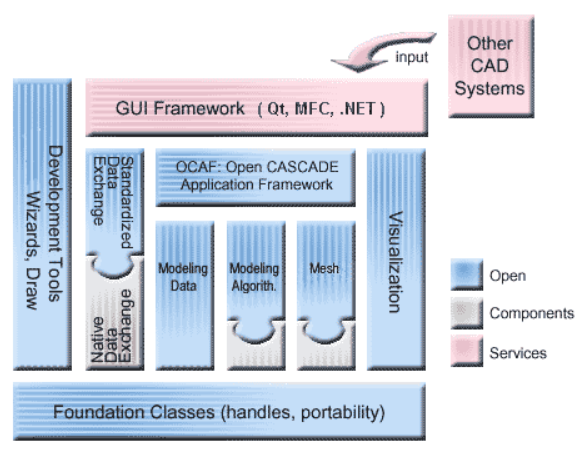
\includegraphics[scale=2.0]{Immagini/Capitolo2/OCCTStructure}
\caption{OCCT module structure}
\label{fig:OCCTStructure}
\end{figure}
%
\noindent
In the following subsections more will be said about the Modeling Data module, the Modeling Algorithms module, and the Data Exchange module, because these are the packages which group the majority of the classes used within \lstinline[language=Java]!JPADCAD!.

\subsection{Modeling Data and Algorithms}
\label{sec2.2.1}

Modeling Data module supplies data structures to implement \gls{BRep} of objects in three dimensions. In \gls{BRep} each shape is an aggregation of geometry within topology. The geometry is the mathematical description of a shape, and it is given by curves and surfaces, which can be of different types (e.g., Bezier, B-Spline, \gls{acr:NURBS}). The topology is a data structure binding geometrical objects together. 

\bigskip
\noindent
On the other hand, Modeling Algorithms module groups a wide range of topological and geometric algorithms used in modeling. These algorithms can be divided in two major groups. The first one comprehends high-level routines used in the real design, such as primitives construction (e.g., boxes, prisms, cylinders), kinematic modeling (e.g., prisms, pipes,), Boolean operations, and algorithms for local modifications (such as hollowing and shelling). The second one groups low-level mathematical support functions, low-level geometric tools, and topological tools providing algorithms to tesselate shapes, convert shapes to \gls{acr:NURBS} geometry, sew connected topologies, etc.

\subsubsection{Geometry}

Geometric entities are grouped in two packages: \lstinline[language=Java]!Geom2d! and \lstinline[language=Java]!Geom!. As the names suggest, \lstinline[language=Java]!Geom2d! package defines geometric objects in 2D space, while \lstinline[language=Java]!Geom! package deals with geometric entities in three dimensions. These packages provide classes for:
%
\begin{itemize}
\renewcommand\labelitemi{$\bullet$}
\item description of points, vectors, curves and surfaces (just \lstinline[language=Java]!Geom!, for obvious reasons);
\item their positioning in the plane/space using coordinates systems;
\item their geometric transformation, by applying translations, rotations, symmetries, scaling transformations and combinations thereof.
\end{itemize}
%
The following geometric objects are available in \gls{OCCT}, with the last four entities pertaining to the \lstinline[language=Java]!Geom! package:
%
\begin{itemize}
\renewcommand\labelitemi{$\bullet$}
\item point,
\item vector,
\item direction,
\item axis,
\item line,
\item conic (circle, ellipse, hyperbola, parabola),
\item bounded curve (trimmed curve, Bezier curve, \gls{acr:NURBS} curve),
\item offset curve,
\item elementary surface (plane, cylinder, cone, sphere, torus),
\item bounded surface (rectangular trimmed surface, Bezier surface, \gls{acr:NURBS} surface),
\item swept surface (surface of linear extrusion, surface of revolution),
\item offset surface.
\end{itemize}
%
One peculiar characteristic of \lstinline[language=Java]!Geom! curves and surfaces is that they are parametrized. For this reason each class comes equipped with functions that allow the user to work with the parametric equation of the curve or surface and to compute the point of a certain parameter u on a curve or the points of parameter $(\text{u}, \text{v})$ on a surface, together with the derivatives (in form of vectors) of every order at this point.

\subsubsection{Topology}

\gls{OCCT} topology allows accessing and manipulating data of objects without dealing with their 2D or 3D representation. Whereas \gls{OCCT} geometry provides a description of objects in terms of coordinates or parametric values, topology describes data structures of objects in parametric space. These description use location in and restriction of parts of this space. Abstract topological data structure describes a basic entity (i.e., a shape), which can be divided into the following component topologies.
%
\begin{itemize}
\renewcommand\labelitemi{\tiny$\blacksquare$}
\item \textbf{Vertex}: a zero-dimensional shape which correspond to a point in geometry.
\item \textbf{Edge}: a shape corresponding to a curve, and bound by a vertex at each extremity.
\item \textbf{Wire}: a sequence of edges connected by their vertices.
\item \textbf{Face}: part of a surface bounded by a closed wire.
\item \textbf{Shell}: a collection of faces connected by some edges of their wire boundaries.
\item \textbf{Solid}: a part of 3D space bound by a shell.
\item \textbf{Solids Compound}: a collection of solids.
\end{itemize}
%
\gls{OCCT} topology is provided by six packages. In the following list, the first three packages describe the topological data structure used in Open CASCADE Technology, while the remaining three provide tools to access and manipulate this topology.
%
\begin{itemize}
\renewcommand\labelitemi{\tiny$\blacksquare$}
\item \textbf{\lstinline[language=Java]!TopAbs!} package groups all the necessary resources for topology-driven applications. It contains enumerations that are used to describe basic topological notions, like topological shape, orientation and state. It also provides methods to manage these enumerations.
\item \textbf{\lstinline[language=Java]!TopLoc!} package provides resources useful to handle 3D local coordinates systems.
\item \textbf{\lstinline[language=Java]!TopoDS!} package contains classes to model and build data structures that are purely topological.
\item \textbf{\lstinline[language=Java]!TopTools!} package provides basic tools to use on topological data structures.
\item \textbf{\lstinline[language=Java]!TopExp!} package provides classes to explore and manipulate the topological data structures contained in the \lstinline[language=Java]!TopoDS! package.
\item \textbf{\lstinline[language=Java]!BRepTools!} package provides classes to explore, manipulate, read and write \gls{BRep} data structures. These more complex data structures combine topological descriptions with additional geometric information, and include rules for evaluating equivalence of different possible representation of the same object.
\end{itemize}
%

\subsubsection{Geometry Utilities}

In order to manage geometry, there are several utilities which provide the following services. Just a few of these tools is contained in the Modeling Data package, while the majority is located in the Modeling Algorithms one.
%
\begin{itemize}
\renewcommand\labelitemi{\tiny$\blacksquare$}
\renewcommand\labelitemii{\tiny$\bullet$}
\item \textbf{Creation of shapes by interpolation and approximation}. In modeling, it is often required to approximate or interpolate points into curves and surfaces. In interpolation, the process is complete when the curve or surface passes through all the points; in approximation, when it is as close to these points as possible. In Open CASCADE, these processes can be performed both in 2D and in 3D, providing the interpolator/approximator method a set of 2D or 3D points. In particular, packages \lstinline[language=Java]!Geom2dAPI! and \lstinline[language=Java]!GeomAPI! provide simple methods for approximation and interpolation with minimal programming. Different types of approximator/interpolator curves can be obtained, such as B-Spline, Bezier and \gls{acr:NURBS}, by simply selecting the right options.
\item \textbf{Direct construction of shapes}. Direct construction methods from \lstinline[language=Java]!gce!, \lstinline[language=Java]!GC! and \lstinline[language=Java]!GCE2d! packages provide algorithms to build elementary geometric entities, such as lines, circles and curves. They complement the reference definitions provided by the \lstinline[language=Java]!gp!, \lstinline[language=Java]!Geom! and \lstinline[language=Java]!Geom2d! packages. The algorithms implemented by \lstinline[language=Java]!gce!, \lstinline[language=Java]!GC! and \lstinline[language=Java]!GCE2d! are simple: there is no creation of objects defined by advanced positional constraints. For example, to construct a circle one could simply provide a point and a radius. The above mentioned simple entities that can be created comprehend:
	%
	\begin{itemize}
	\item 2/3D lines,
	\item 2/3D conics (circles, ellipses, hyperbolae, parabolae),
	\item arcs (of circle, ellipse, parabola, hyperbola),
	\item planes,
	\item cylinders,
	\item cones,
	\item transformations.
	\end{itemize}
	%
\item \textbf{Conversion of curves and surfaces to B-Spline curves and surfaces}. The conversion to and from B-Spline has two distinct purposes. The first one is to provide a homogeneous formulation which can be used to describe any curve or surface. The second one is that it can be used to divide a B-Spline curve or surface into a series of curves or surfaces, thereby providing a higher degree of continuity. All these utilities are grouped in two packages: \lstinline[language=Java]!Geom2dConvert! and \lstinline[language=Java]!GeomConvert!.
\item \textbf{Computation of the coordinates of points on 2D and 3D curves}. \gls{OCCT} gives the user the possibility to use complex algorithms that compute points on a 2D or 3D curve. For example, the following characteristic points exist on parametrized curves in 3D space:
	%
	\begin{itemize}
	\item points equally spaced on a curve,
	\item points distributed along a curve with equal chords,
	\item a point at a given distance from another point on a curve.
	\end{itemize}
	%
Even more options become available by the use of dedicated packages, such as \lstinline[language=Java]!GCPnts!.
\item \textbf{Calculation of extrema between shapes}. The classes to calculate the minimum distance between points, curves, and surfaces, both in 2D and 3D, are provided by \lstinline[language=Java]!Geom2dAPI! and \lstinline[language=Java]!GeomAPI! packages. These packages give the user the capability to calculate the extrema of distance between:
	%
	\begin{itemize}
	\item a point and a curve,
	\item a point and a surface,
	\item two curves,
	\item a curve and a surface,
	\item two surfaces.
	\end{itemize}
	%
\item \textbf{Calculation of intersections between shapes}. Four different types of intersection can be calculated in \gls{OCCT}:
	%
	\begin{itemize}
	\item the intersections between two 2D curves;
	\item the self-intersections of a 2D curve;
	\item the intersection between a 3D curve and a surface;
	\item the intersection between two surfaces.
	\end{itemize}
	%
Intesection between curves in 2D space is managed by the \lstinline[language=Java]!Geom2dAPI_InterCurveCurve! class, while, in 3D space, the intersection between a curve and a surface and two different surfaces is managed, respectively, by the \lstinline[language=Java]!GeomAPI_InterCS! class and the \lstinline[language=Java]!GeomAPI_InterSS! classes.
\item \textbf{Construction of 2D lines and circles from constraints}. \gls{OCCT} provides methods to build, in 2D space, circles and lines using numeric or geometric constraints in relation to other curves. These constraints can impose the following:
	%
	\begin{itemize}
	\item the radius of a circle,
	\item the angle that a straight line makes with another straight line,
	\item the tangency of a straight line or circle in relation to a curve,
	\item the passage of a straight line or circle through a point,
	\item the circle with center in a point or curve.
	\end{itemize}
	%
These algorithms are much more complex than the ones described in the Direct Construction section.
\item \textbf{Construction of curves and surfaces from constraints}. High level functions can be used in \gls{OCCT} in order to create faired and minimal variation 2D curves (\lstinline[language=Java]!FairCurve! package), ruled, pipe and filling of surfaces (\lstinline[language=Java]!GeomFill! package), and plate surfaces (\lstinline[language=Java]!GeomPlate! package).
\item \textbf{Computation of projections}. \gls{OCCT} provides algorithms in order to compute:
	%
	\begin{itemize}
	\item the projections of a 2D point onto a 2D curve;
	\item the projections of a 3D point onto a 3D curve or surface;
	\item the projection of a 3D curve onto a surface.
	\end{itemize}
The classes providing these services are grouped in the \lstinline[language=Java]!Geom2dAPI! and \lstinline[language=Java]!GeomAPI! packages.
\end{itemize}
%

\subsubsection{Topology Tools and Algorithms}

In order to generate topological entities starting from geometric objects or other entities of topological type, the Modeling Algorithms package is provided with different sub-packages, each one specialized in a specific domain. These packages are as follows.
%
\begin{itemize}
\renewcommand\labelitemi{\tiny$\blacksquare$}
\renewcommand\labelitemii{\tiny$\bullet$}
\item \textbf{\lstinline[language=Java]!BRepBuilderAPI!} - Provides classes in order to create \gls{BRep} topology data structure. The \lstinline[language=Java]!BRepBuilderAPI_MakeShape! class is the root of all \lstinline[language=Java]!BRepBuilderAPI! classes, which build shapes. In order to generate an edge element, for example, a \lstinline[language=Java]!BRepBuilderAPI_MakeEdge! object will be created, providing several methods to build an edge from a curve. The \lstinline[language=Java]!BRepBuilderAPI! package also provides classes which allow the creation of connected topology (shells and wires) from a set of separate topological elements (faces and edges). The sewing algorithm is implemented in the class \lstinline[language=Java]!BRepBuilderAPI_Sewing!, which provides methods to load initial data, set customization parameters (such as tolerances), apply analisys methods, and sew the loades shapes.
\item \textbf{\lstinline[language=Java]!BRepFilletAPI!} - Provides classes in order to create fillets and chamfers. A fillet is a smooth face replacing a sharp edge and the class which allows filleting a shape is \lstinline[language=Java]!BRepFilletAPI_MakeFillet!. To produce a fillet it is necessary to define the filleted shape at the construction of the class and add fillet descriptions (such as the radius) using the \lstinline[language=Java]!Add! method. Fillet with changing radius can be also created. On the other hand, a chamfer is a rectilinear edge replacing a sharp vertex of the face and can be performed by using the \lstinline[language=Java]!BRepFilletAPI_MakeChamfer! class. The procedure to produce a chamfer is almost equal to the one for the fillet construction.
\item \textbf{\lstinline[language=Java]!BRepOffsetAPI!} - It groups classes providing the following services:
	%
	\begin{itemize}
	\item creation of offset shapes and their variants, such as hollowing, shelling and lofting;
	\item creation of tapered shapes using draft angles;
	\item creation of sweeps (i.e., objects obtained by sweeping a profile along a path).
	\end{itemize}
	%
\item \textbf{\lstinline[language=Java]!BRepPrimAPI!} - Provides classes for primitives construction, such as boxes, cones, cylinders and prisms. These classes also allow to create partial solids, such as a sphere limited by longitude, and build specific sub-parts by sweeping along a profile (altough for swept constructions along complex profiles such as B-Spline curves the \lstinline[language=Java]!BRepOffsetAPI! package shoul be preferred).
\item \textbf{\lstinline[language=Java]!BRepAlgoAPI!} - This package mainly deals with Boolean operations. Boolean operations are used to create new shapes from the combinations of two shapes. These operations are the most convenient way to create real industrial parts. As most industrial parts consist of several simple elements such as gear wheels, arms, holes, ribs, tubes and pipes, it is usually easy to create those elements separately and then to combine them by Boolean operations in the whole final part. Four operations can be performed, provided by five main classes, of which one (\lstinline[language=Java]!BRepAlgoAPI_BooleanOperation!) is the root:
	%
	\begin{itemize}
	\item \lstinline[language=Java]!BRepPrimAPI_Fuse! performs the fuse operation;
	\item \lstinline[language=Java]!BRepPrimAPI_Common! performs the common operation;
	\item \lstinline[language=Java]!BRepPrimAPI_Cut! performs the cut operation;
	\item \lstinline[language=Java]!BRepPrimAPI_Section! performs the section operation, whose result is a compound made of edges.
	\end{itemize}
	%
In general, Boolean operations can be performed in \gls{OCCT} for various types of arguments. For arguments having the same shape type, for example, the result is a compound, containing shapes of this type. In case of different shape type arguments, some boolean operations can not be performed. For example, the fuse operation between a shell and a solid can not be done, while the cut operation can be performed, provided that the shell is the argument (i.e., the object of the operation) and the solid is the tool.
\item \textbf{\lstinline[language=Java]!BRepFeat!} - This package helps the user for creation and manipulation of form and mechanical features that go beyond the classical boundary representation of shapes. The form features are depressions or protrusions including types such as cylinders, prisms and pipes.
\end{itemize}

\subsection{Data Exchange}
\label{sec2.2.2}

Data Exchange module allows developing \gls{OCCT}-based applications that can interact with other \gls{CAD} systems by writing and reading \gls{CAD} models to and from external data. The exchanges run smoothly regardless of the quality of external data or requirements to its internal representation, for example, to the data types, accepted geometric inaccuracies, etc. Data Exchange module is organized as a set of interfaces that comply with various \gls{CAD} formats: IGES, STEP, STL, VRML, etc. These interfaces allow software based on \gls{OCCT} to exchange data with various \gls{CAD} software packages, mantaining a good level of interoperability.
%
\begin{itemize}
\renewcommand\labelitemi{\tiny$\blacksquare$}
\renewcommand\labelitemii{\tiny$\bullet$}
\item \textbf{Standardized Data Exchange} interfaces allow querying and examining the input file, converting its contents to a \gls{CAD} model and running validity checks on a fully translated shape. The following formats are currently supported:
	\begin{itemize}
	\item STEP (AP203: Mechanical Design; AP214: Automotive Design),
	\item IGES (up to 5.3),
	\item VRML and STL meshes.
	\end{itemize}
\item \textbf{Extended Data Exchange} (XDE) allows translating additional attributes attached to geometric data (colors, layers, names, materials, etc.).
\item \textbf{Advanced Data Exchange Components} are available in addition to Standard Data Exchange interfaces to support interoperability and data adaptation with \gls{CAD} software using the following proprietary formats:
	\begin{itemize}
	\item ACIS SAT,
	\item Parasolid,
	\item DXF.
	\end{itemize}
\end{itemize}
%

\subsection{Open CASCADE Technology Java Wrapper}
\label{sec2.2.3}

The \gls{OCCT} classes are natively written in C++, while \gls{JPAD} is a program written in Java. In order to be able to use the \gls{OCCT} classes in \gls{JPAD}, it is necessary to use a tool that links the two languages. For this purpose, Open CASCADE offers its own Java Wrapper, a tool for wrapping Open CASCADE Technology C++ classes to Java language, to allow their use within Java applications. In particular, the wrapping is made using the \gls{SWIG} tool \cite{webSWIG}. \gls{SWIG} is an interface compiler that connects programs written in C and C++ with languages such as Perl, Python, Java, etc. It works by taking the declarations found in C/C++ header files and using them to generate the wrapper code that other languages need to access the undelying C/C++ code. The Open CASCADE Java Wrapper comes equipped with the \gls{SWIG} interface file (occtypes.i), which contains definitions of basic \gls{OCCT} types for \gls{SWIG} and defines several \gls{SWIG} macros facilitating wrapping of other \gls{OCCT} types. For example, the \texttt{WRAP_AS_ENUM_INCLUDE(name)} macro is uded to wrap enumerations, while \texttt{WRAP_AS_PACKAGE(name)} is used to wrap package methods. The use of these macros allows blind yet customizable approach to wrapping, facilitating controllable but easy wrapping of everything what is needed. The \gls{OCCT} \gls{acr:SDK} currently in use along with the Java wrapper is the 7.0.0 version, altough, at the moment this document is being written, the most recent version is the 7.3.0.

%------------------------------- JPADCAD structure --------------------------------
\section{\texttt{JPADCAD} structure}
\label{sec2.3}

The Open CASCADE Technology library is extremely useful for various reasons, which can be listed as follows:
%
\begin{itemize}
\item supports Manifold and Non-\gls{manifold:geometry};
\item gives the user the possibility to perform \emph{Bottom-Up} construction;
\item has both \gls{CSG} operations and other abstract \emph{feature-like} construction methods;
\item can read and write IGES, STEP and native file formats;
\item is a fully object-oriented \gls{acr:API} with thousands of methods and millions of lines of code.
\end{itemize}
%
The last point is both an advantage and a disadvantage. Having a plethora of methods to chose from surely gives the users all they necessitate to realize the most various applications. On the other hand, the level of programming complexity with the huge suite of methods makes the use of Open CASCADE rather a difficult undertaking. Moreover, its lack of a complete documentation adds to the enormous task of understanding this large but capable software suite. 

\bigskip
\noindent
All of these issues provide the motivation for the design and the development of a system of classes, interfaces and utilities which wrap the original \gls{OCCT} classes, allowing the current and future \gls{JPAD} developers to deal with a lowest number of well documented methods and functions, ready to be used in aerospace \gls{CAD} modeling. The following paragraphs deal with the structure of this system, which, it is good to clarify, is still under costant development. For this reason, some of the most advanced features (for example, those concerning Boolean operations) still need to be adequately wrapped and integrated into the \lstinline[language=Java]!JPADCAD! utilities superstructure.

\subsection{Abstract Factory pattern}
\label{sec2.3.1}

Most of the classes involved in the \gls{OCCT} library wrapping are in the shape domain. As for the \gls{OCCT} library, many topological entities must be managed at the same time in order to build solid models ready to be imported into external tools. The necessity to deal with many different entities all pertinent to the same domain as the possibility to employ, in the next future, geometric modeling kernels other than \gls{OCCT}, has led to the adoption, for the development of the \lstinline[language=Java]!JPADCAD! superstructure, of a particular \gls{design:pattern}. 

\bigskip
\noindent
By definition, \gls{design:pattern}s are reusable solutions to commonly occurring problems in the context of software design \cite{wikiDesignPatterns}. \gls{design:pattern}s were started as best practices that were applied again and again to similar problems encountered in different contexts. They became popular after they were collected, in a formalized form, in the Gang of Four book in 1994. The pattern adopted for \lstinline[language=Java]!JPADCAD! is the one that goes under the name of Abstract Factory pattern. The Abstract Factory pattern offers the interface for creating a family of related objects, without explicitly specifying their classes \cite{wikiAbstractFactoryPattern}. The classes that participate to the Abstract Factory pattern are the followings.
%
\begin{itemize}
\renewcommand\labelitemi{\tiny$\blacksquare$}
\item \textbf{\texttt{AbstractFactory}} - declares an interface for operations that create abstract products.
\item \textbf{\texttt{ConcreteFactory}} - implements operations to create concrete products.
\item \textbf{\texttt{AbstractProduct}} - declares an interface for a type of product object.
\item \textbf{\texttt{Product}} - defines a product to be created by the corresponding \texttt{ConcreteFactory}; it implements the \texttt{AbstractProduct} interface.
\item \textbf{\texttt{Client}} - uses the interfaces declared by \texttt{AbstractFactory} and \texttt{AbstractProduct} classes.
\end{itemize}
%
The \texttt{AbstractFactory} class is the one that determines the actual type of the concrete object and creates it, but it returns an abstract pointer to the concrete object just created. This determines the behavior of the \texttt{Client} that asks the factory to create an object of a certain abstract type and to return the abstract pointer to it, keeping the \texttt{Client} from knowing anything about the actual creation of the object. The fact that the factory returns an abstract pointer to the created object means that the client doesn't have knowledge of the object's type. This implies that there is no need for including any class declarations relating to the concrete type, the client dealing at all times with the abstract type. The objects of the concrete type, created by the factory, are accessed by the \texttt{Client} only through the abstract interface. Figure \ref{fig:AbstractFactoryUML} contains an \gls{acr:UML} diagram which shows how the pattern works. 
%
\begin{figure}[H]
\centering
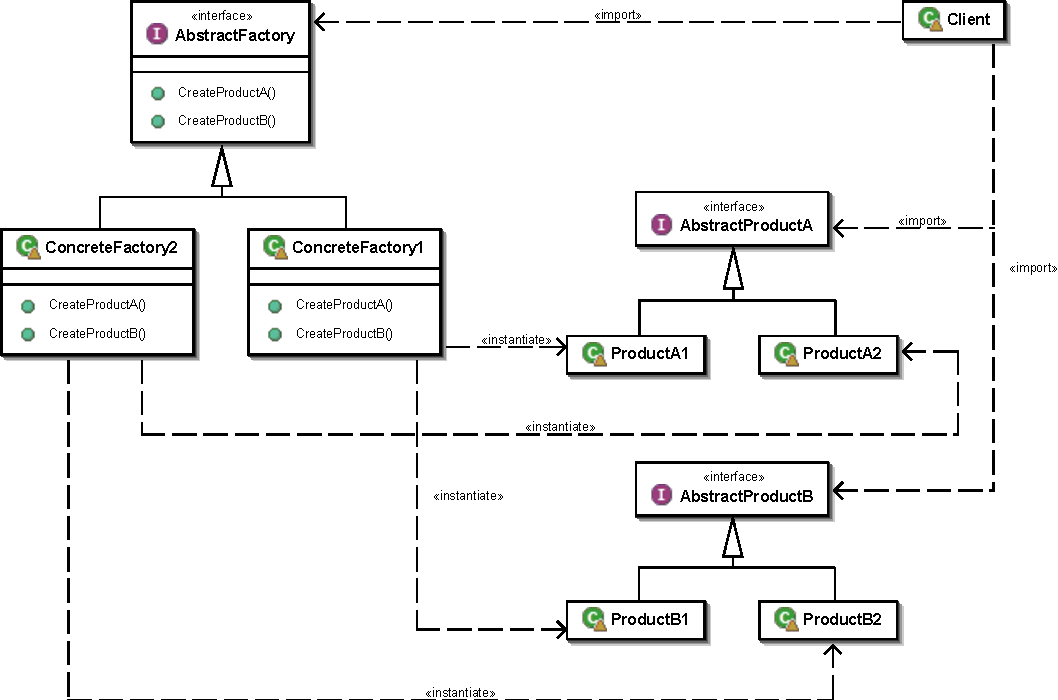
\includegraphics[scale=0.8]{Immagini/Capitolo2/Abstract_factory_UML}
\caption{Abstract Factory pattern \gls{acr:UML}}
\label{fig:AbstractFactoryUML}
\end{figure}
%
\noindent
As figure \ref{fig:AbstractFactoryUML} shows, the \texttt{Client} class that requires the \texttt{ProductA} and \texttt{ProductB} objects doesn't instantiate the \texttt{ProductA1} and \texttt{ProductB1} classes directly. Instead, the \texttt{Client} refers to the \texttt{AbstractFactory} interface for creating objects, which makes the \texttt{Client} independent of how the objects are created (i.e., which concrete classes are instantiated). The \texttt{ConcreteFactory1} class implements the \texttt{AbstractFactory} interface by instantiating the \texttt{ProductA1} and \texttt{ProductB1} classes. Obviously the same can be said for \texttt{ConcreteFactory2}, and \texttt{ProductA2} and \texttt{ProductB2} classes.

\subsection{\texttt{JPADCAD} classes and utilities}
\label{sec2.3.2}

The organizational structure of the \lstinline[language=Java]!JPADCAD! package follows the Abstract Factory pattern paradigm. In the specific case under examination, the abstraction from which all the classes of the package derive consists in considering the package itself as the superstructure of a generic (not better specified) kernel for \gls{CAD} modeling. Therefore, all the classes of the package that have the \lstinline[language=Java]!CAD! prefix are abstract classes (\lstinline[language=Java]!interface! or \lstinline[language=Java]!abstract class! reference types in Java) which therefore need to be implemented. Back to the Abstract Factory pattern, in the case of \lstinline[language=Java]!JPADCAD! the abstract factory is the abstract class \lstinline[language=Java]!CADShapeFactory!. As specified in the previous paragraph, the motivation that led to the use of the Abstract Factory pattern is the possibility that, in the future, more than just one kernel for geometric modeling could be used. Therefore, at present, being \gls{OCCT} the only \gls{CAD} library underlying \gls{JPAD}, the abstract factory \lstinline[language=Java]!CADShapeFactory! has a single implementation, consisting of the \lstinline[language=Java]!OCCShapeFactory! class. In general, all the \lstinline[language=Java]!JPADCAD! classes having the \lstinline[language=Java]!OCC! prefix are concrete classes related to the implementation of the \gls{OCCT} geometric modeling library.

\bigskip
\noindent
\lstinline[language=Java]!JPADCAD! currently comprises almost fourty classes, most of which are related to topological entities. More specifically, these classes can be distinguished as in table \ref{tab:JPADCADclasses}. 
%
\bigskip
\begin{table}[H]
\centering
\begin{tabular}{p{4.0cm}p{10.5cm}}
\toprule
\textbf{Class Type} & \textbf{Characteristics} \\
\midrule
Geometry classes & Define geometric entities (curve, surface) \\[0.5cm]
Shape classes & Define topological entities (vertex, edge, etc.) \\[0.5cm]
Factory classes & Provide factory methods \\[0.5cm]
Explorer classes & Define topological data structure explorers \\[0.5cm]
Iterator classes & Define iterators on sub-shapes \\[0.5cm]
Shape type classes & Provide type-safe enumeration of CAD types \\[0.5cm]
Utility classes & Provide methods to build/manipulate CAD entities \\[0.5cm]
JavaFX export classes & Provide data structure to import shapes into a JavaFX window \\
\bottomrule
\end{tabular}
\caption{\lstinline[language=Java]!JPADCAD! classes and characteristics}
\label{tab:JPADCADclasses}
\end{table}
%

\subsubsection{Shape classes}

Shape classes featured in \lstinline[language=Java]!JPADCAD! follow those offered by \gls{OCCT}, with table \ref{tab:JPADCADTopEnt} showing a comparison between the topology classes of Open CASCADE and the \gls{JPAD} ones. As the table reports, each topological entity has both an interface and its implementation. Moreover, each class specific to a particular topological entity (both interface and concrete class) extends a generic shape class, which is \lstinline[language=Java]!CADShape! for interface classes and \lstinline[language=Java]!OCCShape! for concrete classes. 
%
\bigskip
\begin{table}[H]
\centering
\begin{tabular}{ccc}
\toprule
\textbf{Open CASCADE} & \multicolumn{2}{c}{\textbf{JPAD}} \\
& \textbf{Abstract Topology} & \textbf{Concrete Topology} \\
\midrule
\lstinline[language=Java]!TopoDS_Shape! & \lstinline[language=Java]!CADShape! & \lstinline[language=Java]!OCCShape! \\
\lstinline[language=Java]!TopoDS_Vertex! & \lstinline[language=Java]!CADVertex! & \lstinline[language=Java]!OCCVertex! \\
\lstinline[language=Java]!TopoDS_Edge! & \lstinline[language=Java]!CADEdge! & \lstinline[language=Java]!OCCEdge! \\
\lstinline[language=Java]!TopoDS_Wire! & \lstinline[language=Java]!CADWire! & \lstinline[language=Java]!OCCWire! \\
\lstinline[language=Java]!TopoDS_Face! & \lstinline[language=Java]!CADFace! & \lstinline[language=Java]!OCCFace! \\
\lstinline[language=Java]!TopoDS_Shell! & \lstinline[language=Java]!CADShell! & \lstinline[language=Java]!OCCShell! \\
\lstinline[language=Java]!TopoDS_Solid! & \lstinline[language=Java]!CADSolid! & \lstinline[language=Java]!OCCSolid! \\
\lstinline[language=Java]!TopoDS_CompSolid! & \lstinline[language=Java]!CADCompSolid! & \lstinline[language=Java]!OCCCompSolid! \\
\lstinline[language=Java]!TopoDS_Compound! & \lstinline[language=Java]!CADCompound! & \lstinline[language=Java]!OCCCompound! \\
\bottomrule
\end{tabular}
\caption{\lstinline[language=Java]!JPADCAD! topology classes overview}
\label{tab:JPADCADTopEnt}
\end{table}
%
\noindent
Figure \ref{fig:OCCMap} gives a complete overview on how topology classes are related to each other. Being \lstinline[language=Java]!CADShape! a generic shape interface, it features basic methods common to all type of shapes. These methods are then specified by \lstinline[language=Java]!OCCShape!, using the entities and the algorithms of the \gls{OCCT} library. Table \ref{tab:CADShapeMethods} presents a list of all the methods featured in \lstinline[language=Java]!CADShape!, with a brief explanation for each one. \lstinline[language=Java]!CAD!-type topology interfaces implement the methods in table \ref{tab:CADShapeMethods} yet adding their own ones, specific to the entity they represent. For example, \lstinline[language=Java]!CADEdge! interface extends \lstinline[language=Java]!CADShape! and adds to it methods like \lstinline[language=Java]!range()!, which returns an array containing minimum and maximum values of the parameter describing the geometry of an edge, and \lstinline[language=Java]!vertices()!, that returns the extremities of an edge in terms of \lstinline[language=Java]!CADVertex! entities. In the same way, \lstinline[language=Java]!CADSolid! interface presents its own method which is \lstinline[language=Java]!getVolume()!, that returns the volume of a solid entity. 
%
\begin{figure}[H]
\centering
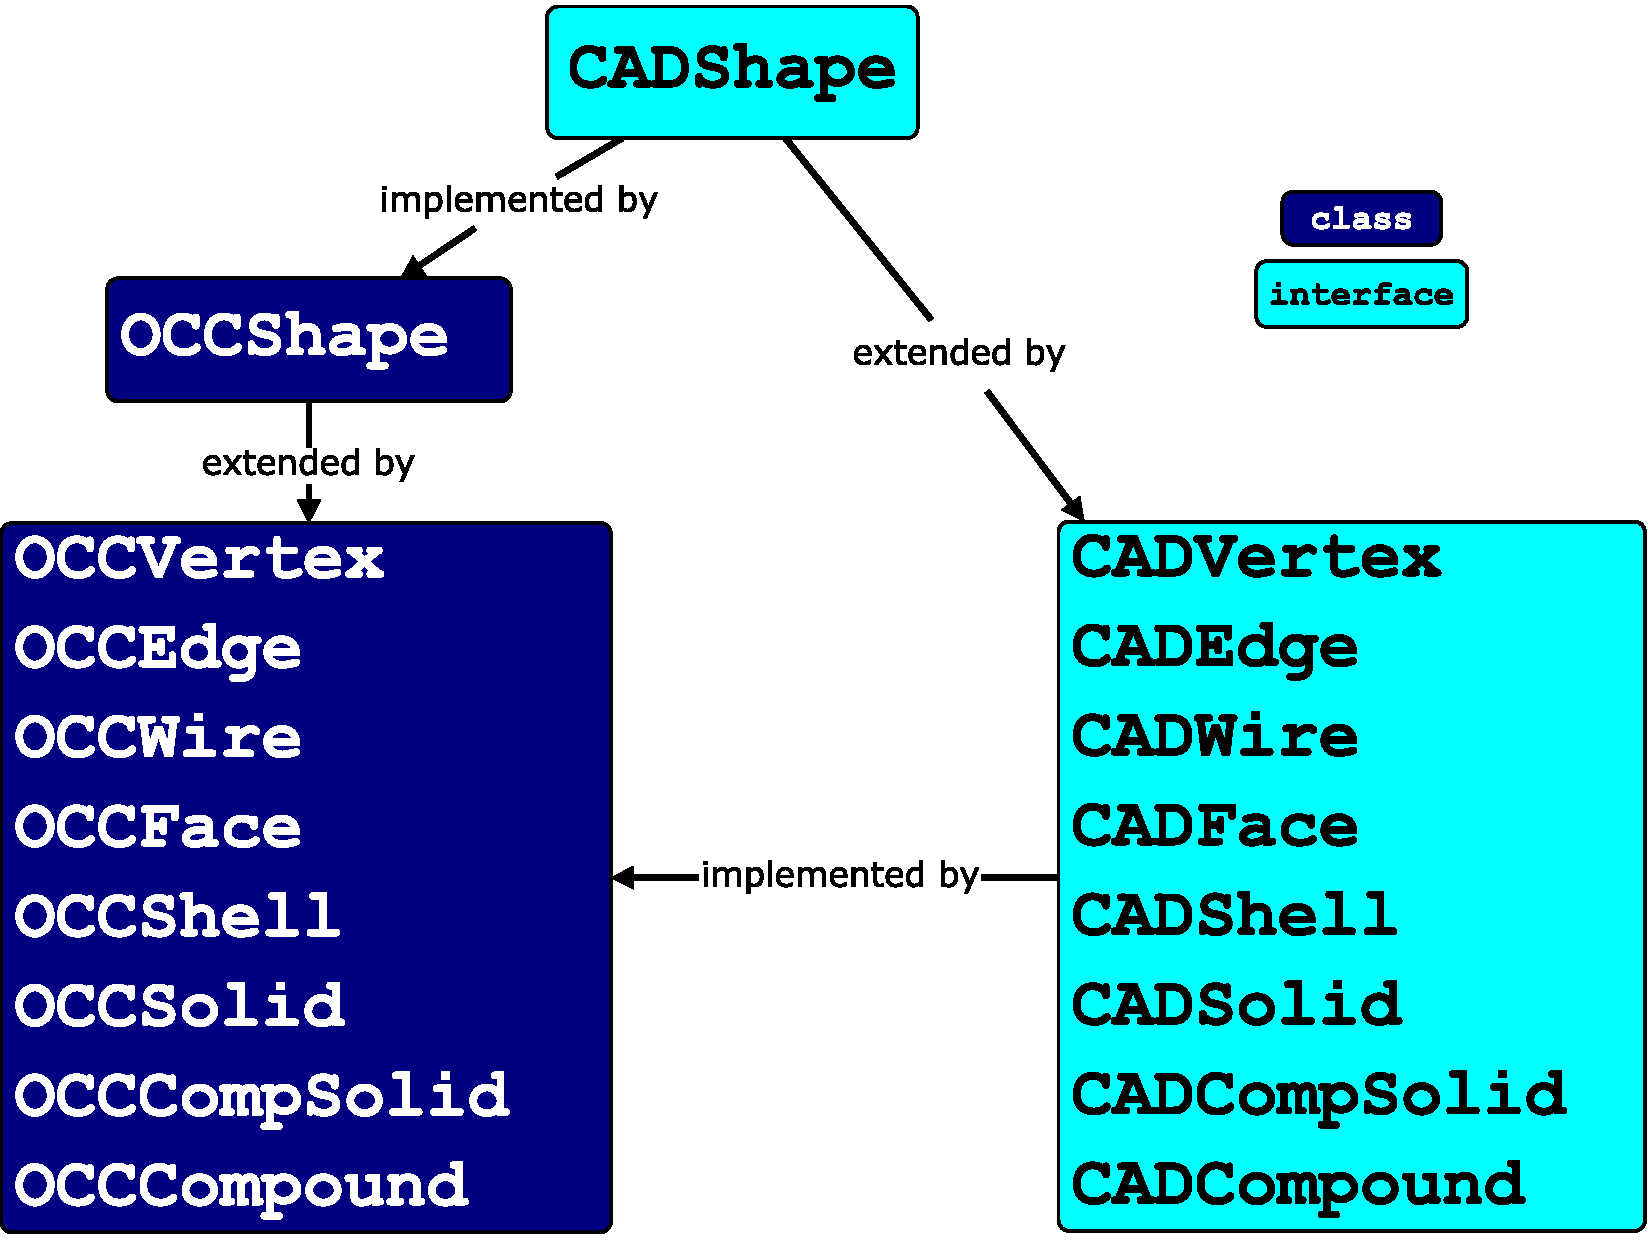
\includegraphics[scale=0.4]{Immagini/Capitolo2/OCCMap}
\caption{Relationship diagram for \lstinline[language=Java]!JPADCAD! topological classes and interfaces}
\label{fig:OCCMap}
\end{figure}
%
\bigskip
\begin{table}[H]
\centering
\begin{tabular}{p{4.2cm}p{10.3cm}}
\toprule
\textbf{Method} & \textbf{Description} \\
\midrule
\lstinline[language=Java]!boundingBox()! & Returns the bounding box of the shape in a \lstinline[language=Java]!double! array format \\[0.2cm]
\lstinline[language=Java]!reversed()! & Returns a reversed instance of the shape \\[0.2cm]
\lstinline[language=Java]!orientation()! & Returns \lstinline[language=Java]!int! value 1 if the shape is forward oriented \\[0.2cm]
\lstinline[language=Java]!isOrientationForward()! & Returns \lstinline[language=Java]!boolean! value \lstinline[language=Java]!true! if the shape is forward oriented \\[0.2cm]
\lstinline[language=Java]!equals(Object o)! & Returns \lstinline[language=Java]!boolean! value \lstinline[language=Java]!true! if \lstinline[language=Java]!o! has same orientation and geometry as the shape \\[0.2cm]
\lstinline[language=Java]!isSame(Object o)! & Returns \lstinline[language=Java]!boolean! value \lstinline[language=Java]!true! if \lstinline[language=Java]!o! has same geometry as the shape \\[0.2cm]
\lstinline[language=Java]!writeNative(String file)! & Writes the shape into the native format \\[0.2cm]
\lstinline[language=Java]!hashCode()! & Returns a hash code matching the equals method \\
\bottomrule
\end{tabular}
\caption{\lstinline[language=Java]!CADShape! methods}
\label{tab:CADShapeMethods}
\end{table}
%
\noindent
As previously stated, \lstinline[language=Java]!OCCShape! generic class implements the \lstinline[language=Java]!CADShape! interface, adding to it also an empty constructor, a shape attribute (of the \lstinline[language=Java]!TopoDS_Shape! type), and setter and getter for the shape attribute. Each \lstinline[language=Java]!OCC! topology class that extends \lstinline[language=Java]!OCCShape! then specifies its own constructors. Listing \ref{lst:shellConstructors} has been included as an example of how shell-type elements can be built, as it reports a partial list of the constructors belonging to this class, plus a private method which provides the actual algorithm through which all the constructors work. The \lstinline[language=Java]!myShape! variable reported in this listing is the previously mentioned shape attribute that each class that extends the \lstinline[language=Java]!OCCShape! one acquires. One thing though should be highlighted: none of the constructors is actually used directly to build new shape objects (as for the shell-type elements as for the others). Following the Abstract Factory pattern, new elements are built through the use of factories and utility classes, as reported in the next paragraphs. 
%
\bigskip
\begin{lstlisting}[caption={\lstinline!OCCShell! constructors and methods}, captionpos=b, tabsize=2, label={lst:shellConstructors}]
public class OCCShell extends OCCShape implements CADShell
{
	// Shell area
	private double area = 0.0;
	
	// Shell builder attributes.
	private static long defaultMakeSolid = 0;
	private static long defaultMakeRuled = 0;
	private static double defaultPrec3D = 1.0e-06;
	
	// Setters and getters
	public static boolean isDefaultMakeSolid() {
			return (defaultMakeSolid == 1);
	}

	public static void setDefaultMakeSolid(boolean value) {
			OCCShell.defaultMakeSolid = (value) ? 1 : 0;
	}

	public static boolean isDefaultMakeRuled() {
			return (defaultMakeRuled == 1);
	}

	public static void setDefaultMakeRuled(boolean value) {
			OCCShell.defaultMakeRuled = (value) ? 1 : 0;
	}

	public static double getDefaultPrec3D() {
			return defaultPrec3D;
	}

	public static void setDefaultPrec3D(double defaultPrec3D) {
			OCCShell.defaultPrec3D = defaultPrec3D;
	}
	
	@Override
	public double getArea() {
			return area;
	}

	// CONSTRUCTORS
	
	/**
	 * Default empty constructor
	 */
	public OCCShell() {
	}	

	/**
	 * Builds a shell through a list of curves
	 */
	public OCCShell(List<CADGeomCurve3D> cadGeomCurveList) {
	
			myShape = OCCShellThruSections(
					null, cadGeomCurveList, null, 
					defaultMakeSolid, defaultMakeRuled, defaultPrec3D
					);
	}

	/**
	 * Builds a shell making it pass through a list of curves and an initial vertex
	 */
	public OCCShell(OCCVertex v0, List<CADGeomCurve3D> cadGeomCurveList) {
	
			myShape = OCCShellThruSections(
					v0, cadGeomCurveList, null, 
					defaultMakeSolid, defaultMakeRuled, defaultPrec3D
					);
	}

	/**
	 * Builds a shell making it pass through a list of curves and a final vertex
	 */
	public OCCShell(List<CADGeomCurve3D> cadGeomCurveList, OCCVertex v1) {
	
			myShape = OCCShellThruSections(
					null, cadGeomCurveList, v1, 
					defaultMakeSolid, defaultMakeRuled, defaultPrec3D
					);
	}
	
	/**
	 * Builds a shell making it pass through a 
	 * list of curves and initial and final vertices
	 */
	public OCCShell(
			OCCVertex v0, List<CADGeomCurve3D> cadGeomCurveList, OCCVertex v1) {
			
			myShape = OCCShellThruSections(
					v0, cadGeomCurveList, v1, 
					defaultMakeSolid, defaultMakeRuled, defaultPrec3D
					);
	}
	
	/**
	 * Actual shell builder, based on OCCT low-level algorithms
	 */
	private TopoDS_Shape OCCShellThruSections(
				OCCVertex v0, List<CADGeomCurve3D> cadGeomCurveList, OCCVertex v1,
				long solid, long ruled, double pres3d) {		
		...
	}
}
\end{lstlisting}
%

\subsubsection{Geometry classes}

\lstinline[language=Java]!JPADCAD! currently comprises six geometry classes, dealing with both 2D and 3D geometric entities. As well as for the shape classes, the \lstinline[language=Java]!CAD! prefix indicates the interfaces dealing with abstract geometry, while the \lstinline[language=Java]!OCC! prefix indicates classes relative to the \gls{OCCT} kernel implementation. Table \ref{tab:JPADCADGeomEnt} gives an overview on the geometry classes contained in \lstinline[language=Java]!JPADCAD!. Another class should be added to this list: \lstinline[language=Java]!OCCDiscretizeCurve3D!. This class, as the name suggests, is pertinent to the \gls{OCCT} implementation and offers support for 3D curves discretization, giving the user the possibility to manipulate curve points.
%
\bigskip
\begin{table}[H]
\centering
\begin{tabular}{ccc}
\toprule
\textbf{Open CASCADE} & \multicolumn{2}{c}{\textbf{JPAD}} \\
& \textbf{Abstract Geometry} & \textbf{Concrete Geometry} \\
\midrule
\lstinline[language=Java]!Geom2dAdaptor_Curve! & \lstinline[language=Java]!CADGeomCurve2D! & \lstinline[language=Java]!OCCGeomCurve2D! \\
\lstinline[language=Java]!GeomAdaptor_Curve! & \lstinline[language=Java]!CADGeomCurve3D! & \lstinline[language=Java]!OCCGeomCurve3D! \\
\lstinline[language=Java]!Geom_Surface! & \lstinline[language=Java]!CADGeomSurface! & \lstinline[language=Java]!OCCGeomSurface! \\
\bottomrule
\end{tabular}
\caption{\lstinline[language=Java]!JPADCAD! geometry classes overview}
\label{tab:JPADCADGeomEnt}
\end{table}
%
\noindent
Basic interfaces contain just the methods, which are then implemented by the \lstinline[language=Java]!OCC! classes by using the \gls{OCCT} functions. These methods are specific for each geometric entity. As an example of this, table \ref{tab:CADGeomSurfMesh} shows the methods contained in \lstinline[language=Java]!CADGeomSurface!, along with a brief description of the operations intended by each one of them.
%
\bigskip
\begingroup
\begin{longtable}[H]{p{5.7cm}p{8.8cm}}
\toprule
\textbf{Method} & \textbf{Description} \\
\midrule
\endfirsthead
%
{\relsize{-1}({\itshape continues from previous page})} & \\
\toprule
\textbf{Method} & \textbf{Description}\\
\midrule
\endhead
%
\midrule 
{\relsize{-1}({\itshape continues on next page})} & 
\endfoot
%
\bottomrule
\caption{\lstinline[language=Java]!CADGeomSurface! methods}
\endlastfoot
%
\lstinline[language=Java]!dinit(int degree)! & Initializes the degree of the surface \\[0.5cm]
\lstinline[language=Java]!value(double u, double v)! & Gets 3D coordinates from $(\text{u}, \text{v})$ coordinates \\[0.5cm]
\lstinline[language=Java]!lowerDistance(double[] p)! & Returns the distance of a point from the surface \\[0.5cm]
\lstinline[language=Java]!setParameter(double u, double v)! & Sets the $(\text{u}, \text{v})$ coordinates used for derivative and curvature operations \\[0.2cm]
\lstinline[language=Java]!d1U()! & Returns the u first derivative vector at the coordinates set by \lstinline[language=Java]!setParameter! \\[0.2cm]
\lstinline[language=Java]!d1V()! & Returns the v first derivative vector at the coordinates set by \lstinline[language=Java]!setParameter! \\[0.2cm]
\lstinline[language=Java]!d2U()! & Returns the u second derivative vector at the coordinates set by \lstinline[language=Java]!setParameter! \\[0.2cm]
\lstinline[language=Java]!d2V()! & Returns the v second derivative vector at the coordinates set by \lstinline[language=Java]!setParameter! \\[0.2cm]
\lstinline[language=Java]!dUV()! & Returns the cross derivative vector at the coordinates set by \lstinline[language=Java]!setParameter! \\[0.2cm]
\lstinline[language=Java]!normal()! & Returns the normal to the surface at the coordinates set by \lstinline[language=Java]!setParameter! \\[0.2cm]
\lstinline[language=Java]!minCurvature()! & Returns the minimum curvature at the coordinates set by \lstinline[language=Java]!setParameter! \\[0.2cm]
\lstinline[language=Java]!maxCurvature()! & Returns the maximum curvature at the coordinates set by \lstinline[language=Java]!setParameter! \\[0.2cm]
\lstinline[language=Java]!gaussianCurvature()! & Returns the Gaussian curvature at the coordinates set by \lstinline[language=Java]!setParameter! \\[0.2cm]
\lstinline[language=Java]!meanCurvature()! & Returns the mean curvature at the coordinates set by \lstinline[language=Java]!setParameter! \\[0.2cm]
\lstinline[language=Java]!curvatureDirections()! & Returns the direction of maximum and minimum curvature at the coordinates set by \lstinline[language=Java]!setParameter!
\label{tab:CADGeomSurfMesh}
\end{longtable}
\endgroup
%
\bigskip
\noindent
Constructors are implemented by the \lstinline[language=Java]!OCC! classes. The most important of these constructors reside in \lstinline[language=Java]!OCCGeomCurve3D!, since the construction of main aircraft components 3D models starts from a series of curves, quite always provided by a good selection of points read from file. \lstinline[language=Java]!OCCGeomCurve3D! actually features three types of constructor, which are partially reported in listing \ref{lst:OCCGC3DCnst} along with some of the attributes and methods of the class. These constructors use classes belonging to the \gls{OCCT} library. In particular, the constructors based on provided point lists perform interpolation through a crucial \gls{OCCT} class, which is \lstinline[language=Java]!GeomAPI_Interpolate!. This class is used to interpolate a B-Spline curve passing through an array of points, with a C2 continuity if tangency is not requested at any middle point. If tangency is requested at some point the continuity will be C1. If periodicity is requested the curve will be closed and the junction will be the first point given.
%
\bigskip
\begin{lstlisting}[caption={\lstinline!OCCGeomCurve3D! constructors}, captionpos=b, tabsize=2, label={lst:OCCGC3DCnst}]
public class OCCGeomCurve3D implements CADGeomCurve3D
{
	// Attributes
	private CADEdge cadEdge = null;
	private GeomAdaptor_Curve myCurve = null;
	private final double[] range = new double[2];
	private OCCDiscretizeCurve3D discret = null;
	private double length = 0.0;
	
	/**
	 * Returns a point on the curve
	 */
	public double[] value(double p) {
			...
	}
	
	/**
	 * Discretizes myCurve splitting it in n arcs. The result is put into discret
	 */
	public void discretize(int n) {		
			...
	}
	
	/**
	 * Returns myCurve range
	 */
	public double[] getRange() {
			return range
	}
	
	/**
	 * Returns myCurve length
	 */
	public double length() {	
			return length;
	}

	/**
	 * Returns the edge element represented by myCurve
	 */
	public CADEdge edge() {	
			return cadEdge;
	}
	
	/**
	 * Returns myCurve
	 */
	public GeomAdaptor_Curve getAdaptorCurve() {	
			return myCurve;
	}
	
	/**
	 * Returns the discretized curve obtained from discretize method
	 */
	public OCCDiscretizeCurve3D getDiscretizedCurve() {	
			return discret;
	}

	// CONSTRUCTORS
	
	/**
	 * Builds a 3D curve from an edge object
	 */
	public OCCGeomCurve3D(CADEdge E) {	
			...
	}
	
	/**
	 * Builds a 3D curve from a list of double[] points. The second  
	 * parameter tells the method whether the curve is periodic or not.
	 */
	public OCCGeomCurve3D(List<double[]> pointsList, boolean isPeriodic) {	
			...	
	}
	
	/**
	 * Builds a 3D curve from a list of double[] points. The second parameter tells 
	 * the method whether the curve is periodic or not, while the third and fourth
	 * parameter set the initial and final tangents, respectively. The last parameter 
	 * tells the method whether the tangents need to be scaled or not. 
	 */
	public OCCGeomCurve3D(List<double[]> pointList, 
			boolean isPeriodic, 
			double[] initialTangent, double[] finalTangent, 
			boolean doScale) {			
			...
	}
}
\end{lstlisting}
%

\subsubsection{Factory and Utility classes}

Factories and utilities are the classes that are actually exploited by \lstinline[language=Java]!JPADCAD! users in order to instantiate new geometric or topological entities. These classes use the aforementioned constructors to build new \gls{CAD} objects. The abstract factory \lstinline[language=Java]!CADShapeFactory! provides the methods that the concrete factory classes must implement. Currently, \lstinline[language=Java]!OCCShapeFactory! is the only implementation provided in \lstinline[language=Java]!JPADCAD!, allowing the construction of 3D \gls{CAD} entities by the use of the \gls{OCCT} classes. Below there is a list of the methods provided by the \lstinline[language=Java]!CADShapeFactory!, along with a description of what they do and the constructors they make use of in the \gls{OCCT} implementation.
%
\begin{itemize}
\renewcommand\labelitemi{\tiny$\blacksquare$}
\renewcommand\labelitemii{\tiny$\bullet$}
\item \textbf{\lstinline[language=Java]!getFactory!, \lstinline[language=Java]!setFactory!} - Getter and setter for the \lstinline[language=Java]!CADShapeFactory! attribute \lstinline[language=Java]!factory!. This attribute needs to be instantiated one time, whenever factory methods are needed.
\item \textbf{\lstinline[language=Java]!newExplorer!, \lstinline[language=Java]!newWireExplorer!} - Methods through which new instances for generic topology explorer (\lstinline[language=Java]!CADExplorer!) and wire explorer (\lstinline[language=Java]!CADWireExplorer!) are created. These explorers are intended for topological data structure investigation. In case of a generic explorer, the shape to explore and the type of the shapes to be found must be provided.
\item \textbf{\lstinline[language=Java]!newIterator!} - Creates a \lstinline[language=Java]!CADIterator! object, intended for sub-shapes iteration.
\item \textbf{\lstinline[language=Java]!newShape!} - Methods that generate \lstinline[language=Java]!CADShape! generic entities. The input provided to the method can be:
	\begin{itemize}
	\item a generic \lstinline[language=Java]!Object! of the underlying implementation (e.g., a \lstinline[language=Java]!TopoDS_Edge! object);
	\item a \lstinline[language=Java]!String! standing for the path to a file, from which \gls{CAD} shapes need to be loaded;
	\item a pair of \lstinline[language=Java]!CADShape! objects and a \lstinline[language=Java]!char!, in order to perform Boolean operations.
	\end{itemize}
In the \gls{OCCT} implementation, Boolean operations are performed thanks to the classes contained in the \lstinline[language=Java]!BRepAlgoAPI! package. The \lstinline[language=Java]!char! parameter allows the user to select the type of the operation to be performed.
\item \textbf{\lstinline[language=Java]!newCurve2D!} - Creates a \lstinline[language=Java]!CADGeomCurve2D! object. Currently the factory contains just one method for 2D curves construction, which needs as input the edge owning the 2D curve and the face (i.e., the plane) containing the same curve.
\item \textbf{\lstinline[language=Java]!newCurve3D!} - Methods used to create \lstinline[language=Java]!CADGeomCurve3D! objects, exploiting the constructors reported in listing \ref{lst:OCCGC3DCnst}. These constructors (and so these methods) allow to generate 3D curves starting from:
	\begin{itemize}
	\item an edge owning the 3D curve;
	\item a pair of points in \lstinline[language=Java]!double[]! format (in order to generate a segment);
	\item an indefinite number (at least two elements) of points in \lstinline[language=Java]!double[]! format;
	\item a list of points in \lstinline[language=Java]!double[]! format;
	\item a list of points in \lstinline[language=Java]!double[]! format, and initial and final tangents in terms of \lstinline[language=Java]!double[]!;
	\item a list of \lstinline[language=Java]!gp_Pnt! (an \gls{OCCT} class used to represent points in 3D space);
	\item a list of \lstinline[language=Java]!PVector! (a class, part of the Java Processing package, which describes two or three dimensional vectors \cite{PVector}).
	\end{itemize}
All the aforementioned methods that generate a 3D curve from points assignment also allow the user to set the curve as periodic.
\item \textbf{\lstinline[language=Java]!newVertex!} - Generates new vertices by providing coordinates in terms of \lstinline[language=Java]!double!.
\item \textbf{\lstinline[language=Java]!newFacePlanar!} - Methods that allow to generate a \lstinline[language=Java]!CADFace! as a planar triangle connecting three vertices. The vertices can be provided both in terms of \lstinline[language=Java]!double[]! points and \lstinline[language=Java]!OCCVertex! entities.
\item \textbf{\lstinline[language=Java]!newShell!} - These methods help the user to build a shell, making it pass through a selected list of curves, and initial and final vertices eventually. The \lstinline[language=Java]!OCCShell! constructors actually allowing the necessary operations have been reported in listing \ref{lst:shellConstructors}. In particular, the \lstinline[language=Java]!newShell! methods enable the user to generate shell elements from the following inputs:
	\begin{itemize}
	\item a list of \lstinline[language=Java]!CADGeomCurve3D!;
	\item an initial \lstinline[language=Java]!CADVertex!, a list of \lstinline[language=Java]!CADGeomCurve3D!, one final \lstinline[language=Java]!CADVertex!.
	\end{itemize}
The \gls{OCCT} class \lstinline[language=Java]!BRepOffsetAPI_ThruSections! provides the algorithms to perform \lstinline[language=Java]!newShell! underlying operations. This class describes functions to build a loft (a shell or a solid entity) passing through a set of sections in a given sequence. It is necessary to point out that none of these methods is used directly to generate shell elements: the \lstinline[language=Java]!OCCUtils! utility class actually contains the methods used in practice, as it will be clear shortly. 
\item \textbf{\lstinline[language=Java]!newShellFromAdjacentFaces!} - It allows to build a shell by connecting adjacent faces. Faces can be provided both in an array of indefinite lenght and in a list. The algorithms that perform the operations in the \gls{OCCT} implementation are provided by the \lstinline[language=Java]!BRepBuilderAPI_Sewing! class.
\item \textbf{\lstinline[language=Java]!newSolidFromAdjacentFaces!} - Performs the same operations described above, producing a solid instead of a shell. In the \gls{OCCT} implementation, the solid is produced by the use of the \lstinline[language=Java]!BRepBuilderAPI_MakeSolid! class.
\end{itemize}
%

\bigskip
\noindent
The concrete factory class \lstinline[language=Java]!OCCShapeFactory!, as long as its methods, are not intended to be instantiated and exploited directly by \lstinline[language=Java]!JPADCAD! users. The utility class \lstinline[language=Java]!OCCUtils!, instead, is intended to be used in order to generate new factory instances through which factory methods can be performed. In particular, \lstinline[language=Java]!OCCUtils! gives the user the capability to make the following operations.
%
\begin{enumerate}
\item Generate a new \lstinline[language=Java]!OCCShapeFactory! instance and assigning it to its own \lstinline[language=Java]!theFactory! attribute, which belongs to the \lstinline[language=Java]!CADShapeFactory! type.
\item Access factory methods through \lstinline[language=Java]!theFactory! attribute, performing the operations on shapes listed above.
\end{enumerate}
%
In addition, \lstinline[language=Java]!OCCUtils! contains several methods covering different necessities that can be encountered while managing \gls{CAD} entities. Though some of these functions just make use of factory methods by simply rearranging the way their parameters are set (as for the methods making use of \lstinline[language=Java]!newShell! factory functions), others allow the users to perform completely new manipulation operations on shapes. Obviously, the methods contained in this utility, as well as the utility class itself, are inherent to the \gls{OCCT} implementation. The following list offers an overview on the methods contained in \lstinline[language=Java]!OCCUtils!.
%
\begin{itemize}
\renewcommand\labelitemi{\tiny$\blacksquare$}
\item \textbf{\lstinline[language=Java]!write!} methods allow to write produced shapes to file. In order to be exported, shapes must be \lstinline[language=Java]!OCCShape! generic instances. The methods currently contained in \lstinline[language=Java]!OCCUtils! allow to write shapes just in BRep format. Other formats, such as STEP and IGES, are actually covered in another utility class, \lstinline[language=Java]!AircraftUtils!, which, at the moment, is contained in \lstinline[language=Java]!JPADCADSandbox!, and whose methods will be explained in the next chapters.
\item \textbf{\lstinline[language=Java]!reportOnShape!} and \textbf{\lstinline[language=Java]!numberOfShapes!} methods enable to investigate shapes, providing a report (viewable on console) on the sub-shapes and their number.
\item \textbf{\lstinline[language=Java]!pointProjectionOnCurve!} methods enable to project points onto a 3D curve, providing \lstinline[language=Java]!CADVertex! entities as result. The \gls{OCCT} class \lstinline[language=Java]!GeomAPI_ProjectPointOnCurve! is behind this operation.
\item \textbf{\lstinline[language=Java]!splitEdge!} functions allow to split edges or curves at one or more locations, returning a list of \lstinline[language=Java]!CADEdge! entities as result. The Open CASCADE class underlying the operations performed by these methods is \lstinline[language=Java]!BOPAlgo_PaveFiller!.
\item \textbf{\lstinline[language=Java]!makeFilledFace!} methods allow the user to generate filling surfaces, i.e., surfaces that can be used to fill empty gaps between faces. These methods make use of the \gls{OCCT} class \lstinline[language=Java]!BRepOffsetAPI_MakeFilling! and \lstinline[language=Java]!newShape! factory methods.
\item \textbf{\lstinline[language=Java]!makePatchThruSections!} routines, finally, make use of \lstinline[language=Java]!newShell! factory methods, in order to enhance user possibilities in terms of which type of parameters can be provided as input in order to generate a shell element from a sequence of points and curves.
\end{itemize}
%

\bigskip
\noindent
The following paragraph shows some simple examples on how \lstinline[language=Java]!JPADCAD! classes are used in order to produce basic shapes. The next chapter will deal on how all the aforementioned methods can be used in order to generate shapes representing more complex geometries, such as those behind main aircraft components.

\subsection{Examples}
\label{sec2.3.3}

The following example shows how to generate B-Spline curves and loft surfaces in \lstinline[language=Java]!JPADCAD!. The methods used below are those descripted in the previous paragraph. Some particular attention has been put on such methods because they are among the most used for aircraft components \gls{CAD} models production. 

\bigskip
\noindent
As previously explained, in order to be able to actually generate \gls{CAD} shapes in \gls{JPAD} it is necessary to instantiate a factory. For this reason, the first method called through \lstinline[language=Java]!OCCUtils! is \lstinline[language=Java]!initCADShapeFactory!. After making sure that a \lstinline[language=Java]!OCCShapeFactory! instance actually exists, the first thing to do is creating points for the curves. In the listing below, these points are created in \lstinline[language=Java]!double[]! format, and passed to the \lstinline[language=Java]!newCurve3D! method, along with a \lstinline[language=Java]!boolean! value that states that the curve we want to generate is not periodic. The application of the previous method returns a generic \lstinline[language=Java]!CADGeomCurve3D!, as required by the use of the Abstract Factory pattern. Exploiting the \lstinline[language=Java]!edge! method provided by the \lstinline[language=Java]!CADGeomCurve3D! interface, the \lstinline[language=Java]!CADEdge! entity underlying the B-Spline curve can be obtained.
%
\bigskip
\begin{lstlisting}[caption={B-Spline curve creation}, captionpos=b, tabsize=2, label={lst:Example1}]		
		if(OCCUtils.theFactory == null) 
			OCCUtils.initCADShapeFactory();
		
		// Create a list of points to be passed to the 
		// factory methods for 3D curves generation
		double[] pntA = new double[] {0.0, -1.0, 0.0};
		double[] pntB = new double[] {0.0,  0.0, 1.0};
		double[] pntC = new double[] {0.0,  2.0, 0.0};
		
		// Generate a B-Spline curve from the previous points
		CADGeomCurve3D curve1 = OCCUtils.theFactory.newCurve3D(false, pntA, pntB, pntC);
		
		// Get the edge entity underlying the previous curve
		CADEdge edge1 = curve1.edge();
\end{lstlisting}
%
\bigskip
\noindent
In order to produce other curves and to show how \lstinline[language=Java]!newCurve3D! can actually manage more than just one set of parameters (thanks to Java polymorphism), the previous points are added to a Java \gls{List} \cite{JavaList} and manipulated (after being inserted in the list), in order to generate the successive curves at a certain distance from the previous one. In this way, two more curves are made, with the last one being also imposed two tangency constraints, at the initial and final point respectively. Once all the curves are made, the \lstinline[language=Java]!write! method is called by the use of \lstinline[language=Java]!OCCUtils!, allowing to write the desired shapes to a BRep file. The result is shown in figure \ref{fig:EdgeExample}.
%
\bigskip
\begin{lstlisting}[caption={B-Spline curve creation with different \lstinline!newCurve3D! methods}, captionpos=b, tabsize=2, label={lst:Example2}]		
		// Passing points to the B-Spline curves generator method through a Java List
		List<double[]> points1 = new ArrayList<double[]>();
		
		points1.add(pntA);
		points1.add(pntB);
		points1.add(pntC);		
		points1.forEach(d -> d[0] = 2.0);
		
		CADGeomCurve3D curve2 = OCCUtils.theFactory.newCurve3D(points1, false);
		
		// Get the edge entity underlying the previous curve
		CADEdge edge2 = curve2.edge();
		
		// Give to the B-Spline factory method initial and final tangent too
		List<double[]> points2 = new ArrayList<double[]>();
		
		points2.addAll(points1);
		points2.forEach(d -> d[0] = 10.0);
		
		double[] iTang = new double[] {0.0, 1.0, 0.0};
		double[] fTang = iTang;
		
		CADGeomCurve3D curve3 = OCCUtils.theFactory.newCurve3D(points2, 
				false, 
				iTang, fTang, 
				false
				);
		
		// Get the edge entity underlying the previous curve
		CADEdge edge3 = curve3.edge();
		
		// Writing the generated edges to BRep file
		System.out.println("Have been the shapes correctly written to file? " + 
				OCCUtils.write("EdgeExample_01.brep", 
						(OCCEdge) edge1, 
						(OCCEdge) edge2,
						(OCCEdge) edge3
						));
\end{lstlisting}
%
\bigskip
\noindent
The last part of the example focuses on \lstinline[language=Java]!newShell! and \lstinline[language=Java]!makePatchThruSections! methods. The curves used as sections for the loft are those created in the first part of the example. Three lofts are made, exploiting three \lstinline[language=Java]!makePatchThruSections! available variants. The example also shows how to generate \lstinline[language=Java]!CADVertex! entities by use of a \lstinline[language=Java]!double! array. Generated shapes are then transcripted to file and reported in figures \ref{fig:ShellExample1}, \ref{fig:ShellExample2} and \ref{fig:ShellExample3}.
%
\bigskip
\begin{lstlisting}[caption={Lofts creation by use of \lstinline!makePatchThruSections! methods}, captionpos=b, tabsize=2, label={lst:Example3}]	
		// Making a shell pass through the curves
		OCCShape shell1 = OCCUtils.makePatchThruSections(curve1, curve2, curve3);
		
		// Writing the generated shell to BRep file
		System.out.println("Have been the shapes correctly written to file? " + 
				OCCUtils.write("ShellExample_01.brep", shell1));
					
		// Making a shell pass through the above generated curves and an initial vertex
		List<CADGeomCurve3D> curves = new ArrayList<CADGeomCurve3D>();
		
		curves.add(curve1);
		curves.add(curve2);
		curves.add(curve3);
		
		CADVertex iVtx = OCCUtils.theFactory.newVertex(new double[] {-10.0, 0.0, 0.0});
		
		OCCShape shell2 = OCCUtils.makePatchThruSections(iVtx, curves);
		
		// Writing the generated shell to BRep file
		System.out.println("Have been the shapes correctly written to file? " + 
				OCCUtils.write("ShellExample_02.brep", shell2));
		
		// Making a shell pass through initial and final vertices too
		CADVertex fVtx = OCCUtils.theFactory.newVertex(new double[] {20, 0.0, 0.0});

		OCCShape shell3 = OCCUtils.makePatchThruSections(iVtx, curves, fVtx);

		// Writing the generated shell to BRep file
		System.out.println("Have been the shapes correctly written to file? " + 
				OCCUtils.write("ShellExample_03.brep", shell3));		
\end{lstlisting}
%
\begin{figure}[!ht]
\centering
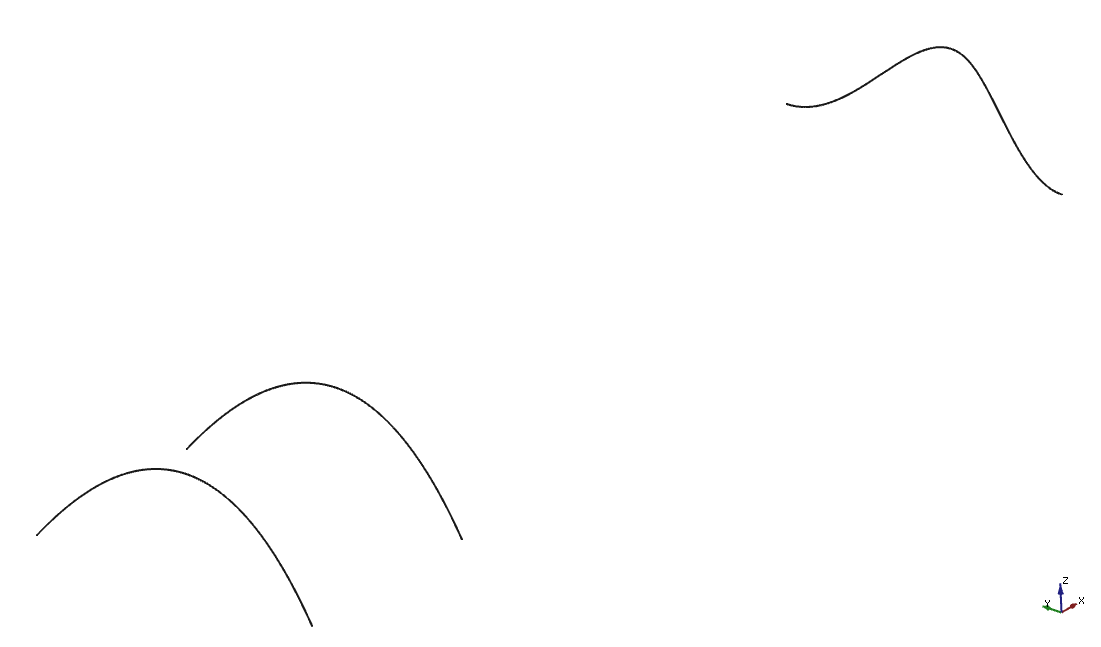
\includegraphics[scale=0.5]{Immagini/Capitolo2/EdgeExample2}
\caption{Edges obtained by use of \lstinline[language=Java]!newCurve3D! methods}
\label{fig:EdgeExample}
\end{figure}
%
%
\begin{figure}[!ht]
\centering
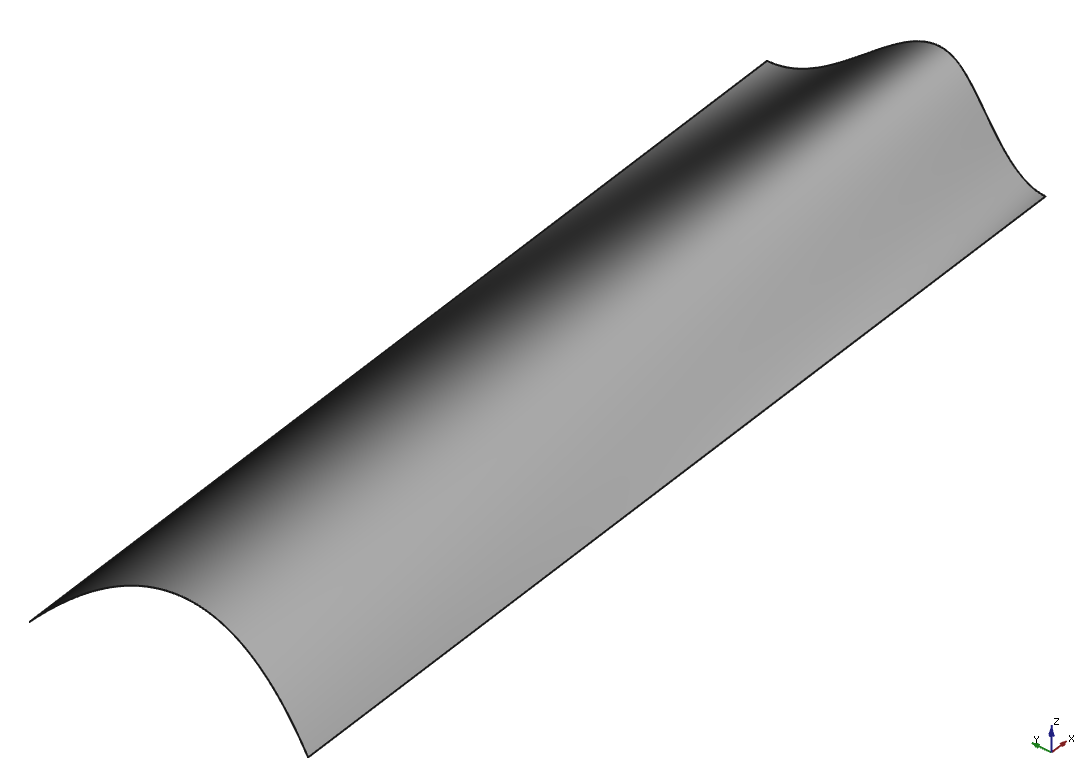
\includegraphics[scale=0.5]{Immagini/Capitolo2/ShellExample12}
\caption{Loft passing through three curves}
\label{fig:ShellExample1}
\end{figure}
%
%
\begin{figure}[!ht]
\centering
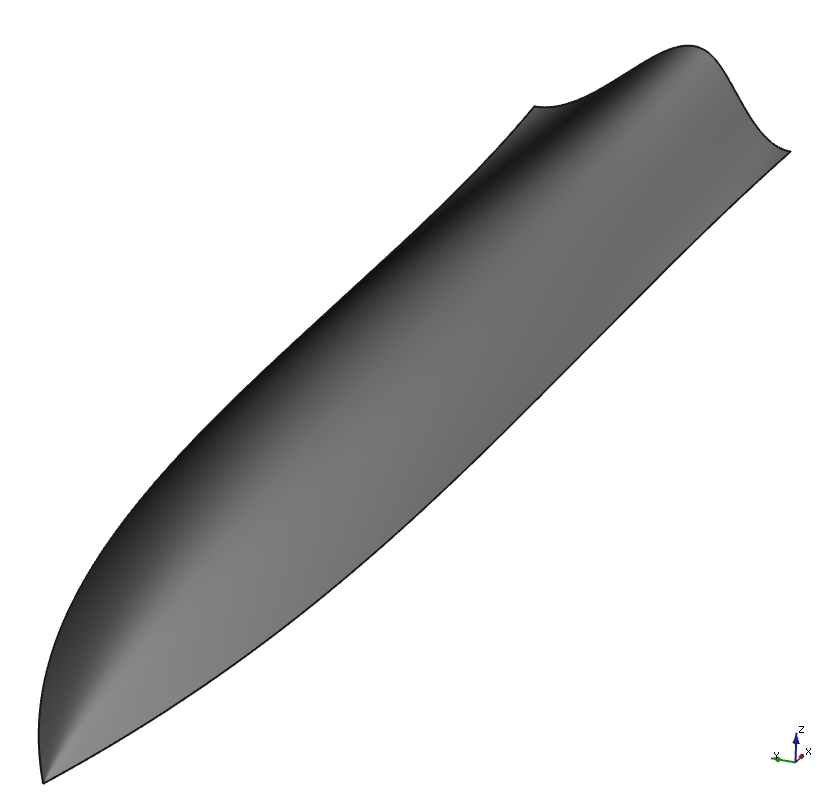
\includegraphics[scale=0.6]{Immagini/Capitolo2/ShellExample22}
\caption{Loft passing through three curves and an initial vertex}
\label{fig:ShellExample2}
\end{figure}
%
%
\begin{figure}[!ht]
\centering
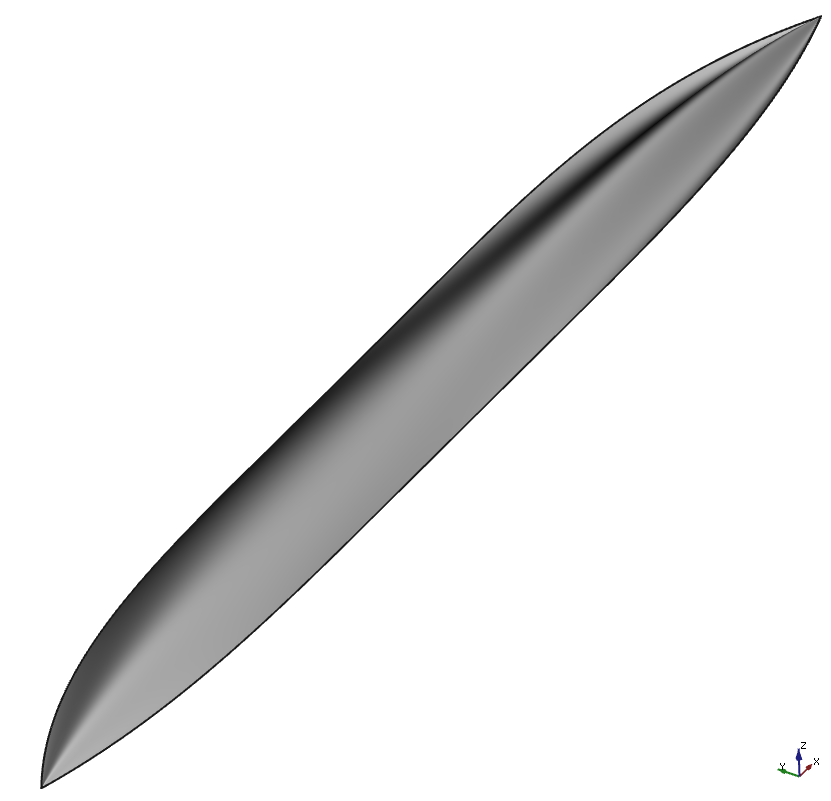
\includegraphics[scale=0.6]{Immagini/Capitolo2/ShellExample32}
\caption{Loft passing through three curves and initial and final vertices}
\label{fig:ShellExample3}
\end{figure}
%
\chapter{A utility class for aircraft modeling: \texttt{AircraftUtils}}
\label{chap3}

\section{Introduction}
\label{sec3.1}

Once the \lstinline[language=Java]!JPADCAD! library was developed, providing basic methods for the construction of \gls{CAD} shapes, these same methods have been used to create functions that, starting from the geometric characteristics of a given aeronautical component supplied in input, automatically generate the \gls{CAD} model of the aircraft, complete of all of its components or just a given number of them. As stated in Chapter \ref{chap1}, \gls{JPAD} comes equipped with classes and methods that allow to read data regarding the aircraft and its components from appropriately formatted XML files. Reading this data determines the creation of an instance of the \gls{JPAD} \lstinline[language=Java]!Aircraft! class. This class is the one delegated to the storage of all the data related to the aircraft, and also contains all the methods that allow access to the different sub-components of the airplane. These sub-components are treated in \gls{JPAD} by the use of different classes. As for the sub-components currently modeled through the use of \lstinline[language=Java]!JPADCAD!, the \lstinline[language=Java]!Fuselage! and \lstinline[language=Java]!LiftingSurface! classes are those delegated to the description, respectively, of the fuselage and all the different types of aerodynamic components in general. For this reason, the \lstinline[language=Java]!LiftingSurface! class can be used, for example, to describe both wings and tail surfaces. The modeling of the \gls{CAD} entities of the different components of an aircraft starts from the instances of these classes, as it will be more evident in the next paragraphs.

\section{\texttt{AircraftUtils} overview}
\label{sec3.2}

In order to develop and test methods allowing the construction, from scratch, of aircraft principal components, a new package has been added to the \gls{JPAD} three. This package, named \lstinline[language=Java]!JPADCADSandbox!, has been conceived with the intent to build some sort of \emph{playground} for all the activities inherent to \gls{CAD} modeling. For this reason, this package not only contains the test classes produced to check the correct functioning of the methods contained in \lstinline[language=Java]!JPADCAD!. On the contrary, at present, it also contains all the methods used to build the 3D counterparts of the instances of the \lstinline[language=Java]!Fuselage! and \lstinline[language=Java]!LiftingSurface! classes. These methods have all been collected in one class, along with others that will be listed in the following, which serves as an utility class, i.e., a class that does not need to be instantiated and provides several methods for multiple other classes. These methods can then be accessed in a static way, providing an approach to the solution of a problem which is not properly object oriented (like should be when using a programming language such as Java), but that produces easy to debug/mantain code, which is an important prerequisite especially when developing new functionalities. This utility class is called \lstinline[language=Java]!AircraftUtils! and, along with the methods that have been referred very briefly above, it also provides functions that can be used to:
%
\begin{itemize}
\item load an aircraft from XML file;
\item write aircraft solid components to file;
\item get the whole aircraft shapes.
\end{itemize}
%
All these methods are set to public, meaning that they can be actually accessed by external classes. Furthermore, \lstinline[language=Java]!AircraftUtils! contains several private methods (i.e., functions that can be used only by classes and methods internal to the class in which they are defined), that provide support when dealing, for example, with the wing tip building. Finally, it also includes some enumeration classes, dealing with file extension and spacing type. These enumerators are mainly used internally \lstinline[language=Java]!AircraftUtils!, and more will be said about them and all the public extra methods in paragraph \ref{sec3.5}. 

\bigskip
\noindent
The next two paragraphs, instead, deal with the methodologies and the functions used to build main aircraft components: the fuselage and the lifting surfaces. In order to build these components properly, some sort of construction strategy must be followed. This is a crucial point, especially when dealing with the necessity of using the same code for the construction of the most various shapes and configurations. For this reason, the typical modeling strategies for aircraft geometric design were adopted \cite{paperCADinAero}, by making use of all the primary functions generally used when dealing with object such as fuselages and wings. Classically, typical aircraft components are modeled by means of loft functions. This type of functions, that have been described in paragraph \ref{sec2.3.2} along with their implementation in \lstinline[language=Java]!JPADCAD!, usually requires planar section curves, plus guide curves in some cases (actually not the underlyng \gls{OCCT} algorithm used for the \lstinline[language=Java]!ThruSections! methods), to build shapes that could not be obtained by use of simple extrude, revolve or sweep functions. When dealing with aircraft geometric modeling, loft functions are undoubtedly the most used ones. In order to actually use these functions, it is necessary to construct a wireframe first. This wireframe consists of a set of primary shapes (basically curves or wires) that helps building the final 3D model and provides a first glimpse at the result we coming up with. In aircraft modeling, two different types of primary shapes exist: wing-type shapes and fuselage-type shapes. In case of wing-type shapes the defining sections are parallel to the flow direction and are tipically airfoils, while in case of fuselage-type shapes the defining sections are normal to the flow direction and are symmetrical. Once the wireframes have been defined lofting operations can begin, giving life to the succession of steps that will lead to the generation of the definitive 3D model of the aeronautical component. The methods described below, which return the shapes of primary aircraft components, follow the just described methodology. The next paragraphs therefore provide a focus on how these steps are followed and which classes and methods the construction functions make use of. Moreover, when explaining the algorithms behind the creation of the 3D model of a lifitng surface, a particular emphasis will be given to the methodology followed for the generation of the wing tip, which is the element of greater complexity of the 3D wing produced by \gls{JPAD}. 

\section{Fuselage CAD method}
\label{sec3.3}

In order to help the subsequent lofting operations, it was first necessary to conceive a subdivision of the surface of the fuselage. Thankfully \gls{JPAD} \lstinline[language=Java]!Fuselage! class helps doing this by providing a schematization of the external surface which can be easily used for \gls{CAD} purposes. This scheme splits the fuselage in five principal parts, which can be listed as follows:
%
\begin{itemize}
\item nose cap,
\item nose trunk,
\item cylindrical trunk,
\item tail trunk,
\item tail cap.
\end{itemize}
%
When coming to the \gls{CAD} generation problem, one could imagine each of the parts mentioned above having its own patch being produced by means of a lofting method. The union of these patches (obtained by the use of sewing algorithms) determines the final shape of the fuselage (figure \ref{fig:FusInfographic}). This subdivision not only helps building lofts representing the external surface, making the patching through sections phase much easier. It also provides an useful scheme that has been actually used to fix the parameters of the algorithm for the fuselage construction. The method doing this is called \lstinline[language=Java]!getFuselageCAD! and the parameters it accepts are the followings.
%
\begin{itemize}
\renewcommand\labelitemi{\tiny$\blacksquare$}
\renewcommand\labelitemii{\tiny$\bullet$}
\item \textbf{\lstinline[language=Java]!fuselage!} - An instance of the \lstinline[language=Java]!Fuselage! type containing all the geometric information about the component. It provides easy access to the lists of points defining side curves and outlines. It also contains methods returning the $x$-coordinates of the sections delimiting one part of the fuselage from another.
\item \textbf{\lstinline[language=Java]!noseCapSectionFactor1!, \lstinline[language=Java]!noseCapSectionFactor2!} - Entries defining the limits, in terms of $x$-coordinates, of the nose cap patch. In particular, these factors (which are expressed as Java \lstinline[language=Java]!double!) multiply the nose cap offset length normalized with respect to the nose length, thus returning the normalized initial and terminal $x$-coordinates of the sections defining the shape of the nose cap. 
\item \textbf{\lstinline[language=Java]!numberNoseCapSections!} - An \lstinline[language=Java]!int! fixing the number of nose cap sections to patch through. 
\item \textbf{\lstinline[language=Java]!numberNosePatchSections!} - An \lstinline[language=Java]!int! defining the number of nose trunk sections.
\item \textbf{\lstinline[language=Java]!spacingTypeNosePatch!} - An instance of one of the Java \lstinline[language=Java]!enum! classes mentioned above, defining the type of spacing to be adopted for the sections of the nose trunk. 
\item \textbf{\lstinline[language=Java]!numberTailPatchSections!} - An \lstinline[language=Java]!int! value defining the number of sections to be created for the tail trunk.
\item \textbf{\lstinline[language=Java]!spacingTypeTailPatch!} - The spacing type for the tail trunk sections.
\item \textbf{\lstinline[language=Java]!tailCapSectionFactor1!, \lstinline[language=Java]!tailCapSectionFactor2!} - What has been said for the nose cap sections applies here. These factors simply fix the $x$-coordinates of the tail cap initial and terminal sections.
\item \textbf{\lstinline[language=Java]!numberTailCapSections!} - An \lstinline[language=Java]!int! value fixing the number of tail cap sections to patch through.
\item \textbf{\lstinline[language=Java]!exportSupportShapes!, \lstinline[language=Java]!exportLofts!, \lstinline[language=Java]!exportSolids!} - Entries of the Java \lstinline[language=Java]!boolean! type, allowing the user to select which kind of shapes he wants to generate and export, with the shapes being respectively: support shapes, such as those defining the wireframe of the fuselage; loft shapes, generated by patching through the fuselage sections; solid shapes, obtained by sewing the lofts.
\end{itemize}
%
\begin{figure}[H]
\centering
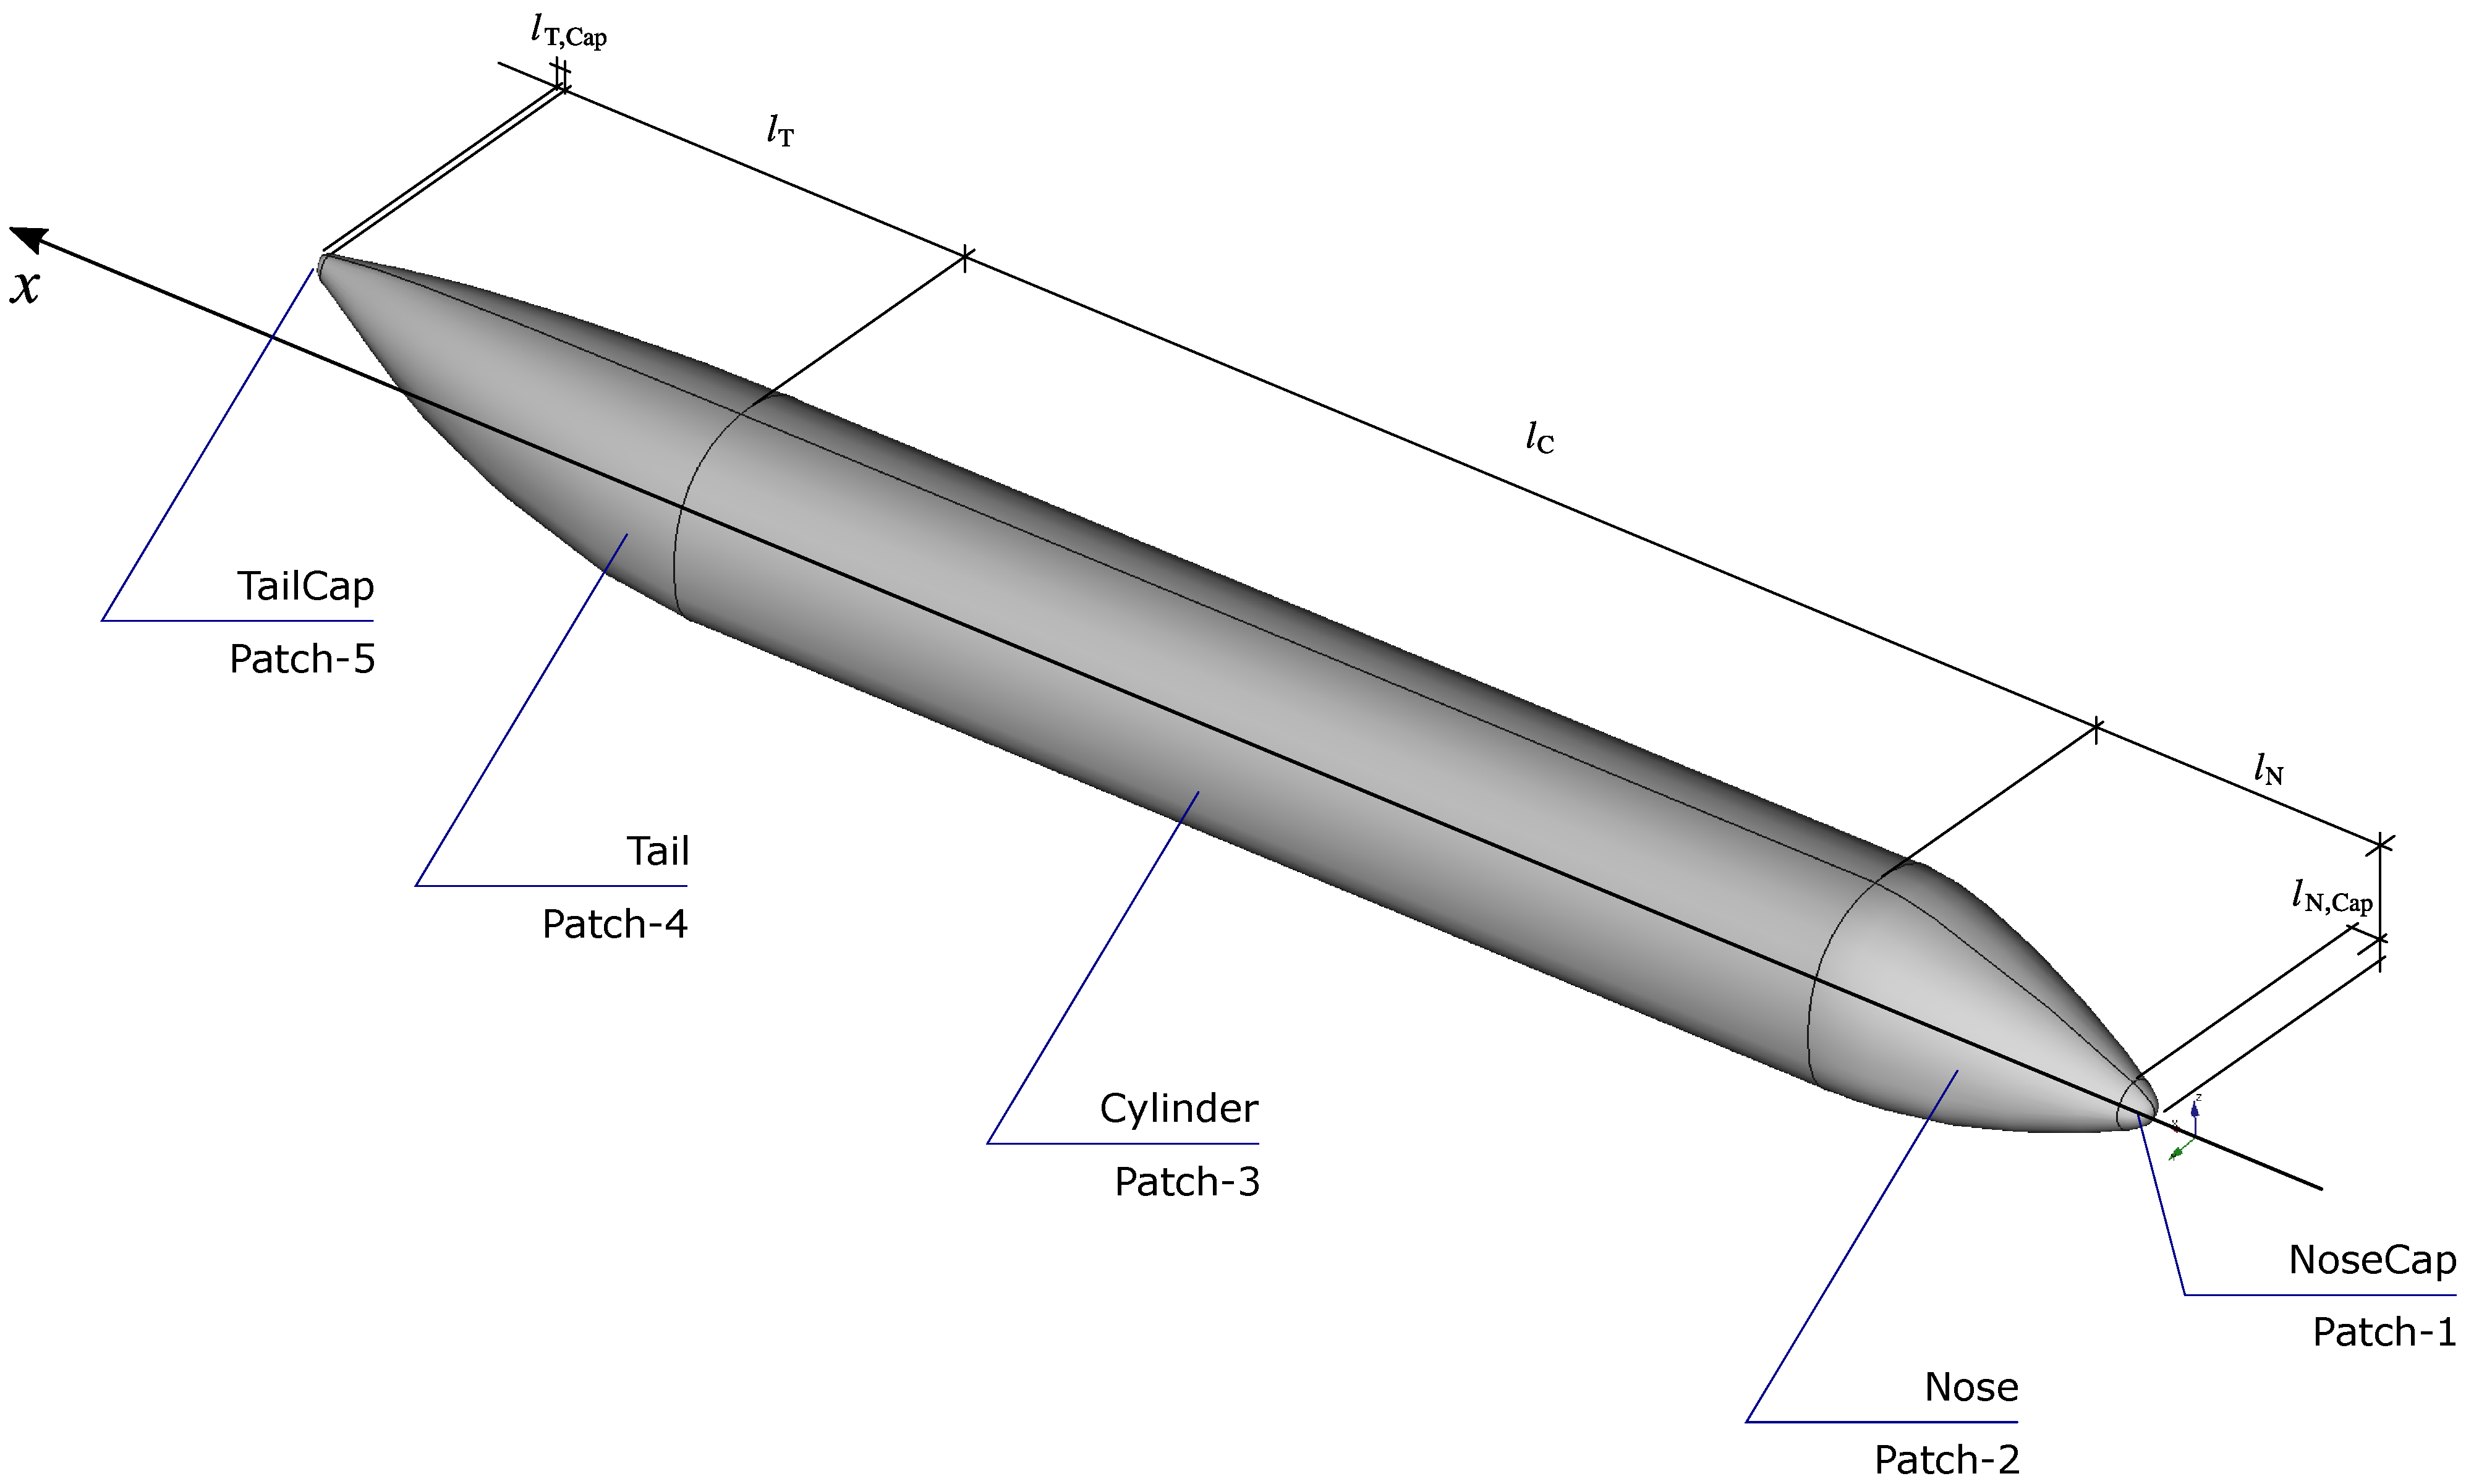
\includegraphics[scale=0.22]{Immagini/Capitolo3/fuselage_1}
\caption{Fuselage schematization for CAD purposes}
\label{fig:FusInfographic}
\end{figure}
%

\bigskip
\noindent
The algorithm can be split in two sections, with the first one providing for the generation of the lofts and the solid, while the second one is mainly dedicated to the production of the outline curves of the fuselage, completing the list of the extra shapes to be exported in case the \lstinline[language=Java]!exportSupportShapes! variable has been set to \lstinline[language=Java]!true!. After collecting essential geometric variables (such as those related to the lengths of the parts in which the fuselage has been split), the construction of the five patches that compose the fuselage begins. The building process clearly starts from the nose cap and continues till the terminal section of the fuselage.

\bigskip
\noindent
In order to determine the curves to patch through, the $x$-coordinates of the sections must be first calculated. As anticipated, the \lstinline[language=Java]!noseCapSectionFactor1! and \lstinline[language=Java]!noseCapSectionFactor2! parameters fix the position of the initial and terminal section of the nose cap patch. In particular, when respectively fixed to $0.0$ and $1.0$, first and last nose cap patch sections $x$-coordinates coincide with the actual initial and teminal $x$-coordinates of the nose cap. In order to avoid a degenerate section, the first parameter must be set to a value higher than $0.0$ (usually a value equal to $0.15$ seems to work fine). The number of nose cap sections provided to the algorithm determines how many $x$-coordinates must be calculated between initial and terminal ones, with the spacing between the sections being set to half-cosine type (with higher density towards the terminal section). \gls{JPAD} utility class \lstinline[language=Java]!MyArrayUtils! provides methods for spacing. Once all the $x$-coordinates have been determined, it is finally possible to acquire section points, by means of the \lstinline[language=Java]!Fuselage.getUniqueValuesYZSideRCurve! method. It requires the $x$-coordinates of the sections expressed in terms of \lstinline[language=Java]!Amount! (a Java class, part of the JScience package, providing support for measurements \cite{Amount}) values, and returns a list of \lstinline[language=Java]!PVector! entities, representing the coordinates of the fuselage side curve points. As the name of the method suggests, just the right curve points are returned, given the simmetry of the fuselage. For this reason, mirroring operations must be performed on lofts in order to obtain the complete shape of the fuselage, as it will be clarified in the following. Once all the lists of \lstinline[language=Java]!PVector! points have been collected, the patch for the nose cap can be finally obtained, by means of one of the \lstinline[language=Java]!OCCUtils! methods listed in Chapter \ref{chap2}. Since the patch needs to be made pass through one initial vertex and a set of curves defined by means of \lstinline[language=Java]!PVector! entities, an appropriate variant of the \lstinline[language=Java]!makePatchThruSections! methods has been used. Listing \ref{lst:NoseCapCreation} contains pieces of the actual code used to generate nose cap shapes. Variables containing the term \lstinline[language=Java]!bar! in their name hint at quantities which have been normalized with respect to the whole nose length, as specified above. 
%
\bigskip
\begin{lstlisting}[caption={Nose cap shapes building process}, captionpos=b, tabsize=2, label={lst:NoseCapCreation}]
// Determine a List containing the sections x-coordinates normalized with  
// respect to the nose length. xbarNoseCap is the normalized nose cap length. 
List<Double> xbars1 = Arrays.asList(
				MyArrayUtils
					.halfCosine2SpaceDouble(
					noseCapSectionFactor1*xbarNoseCap, noseCapSectionFactor2*xbarNoseCap, 
					numberNoseCapSections) 
				);
				

// Fill a List of PVectors for each section
List<List<PVector>> sections1 = new ArrayList<List<PVector>>();
xbars1.forEach(x -> sections1.add(
				 fuselage.getUniqueValuesYZSideRCurve(noseLength.times(x)))
	  );
	  
	
// Generate the patch for the nose cap
PVector noseTipVtx = new PVector(0.0f, 0.0f, (float) zNoseTip.doubleValue(SI.METER))	  
OCCShape patch1 = OCCUtils.makePatchThruSectionsP(
							noseTipVtx,
							sections1
							);
						
// Actually generate the supporting curves and add them to the ones to be exported
sections1.stream()
			.map(sec -> OCCUtils.theFactory
					.newCurve3D(
							sec.stream()
							.map(p -> new double[] {p.x, p.y, p.z})
							.collect(Collectors.toList()),
							false)
					)
			.map(crv -> (OCCEdge) ((OCCGeomCurve3D) crv).edge())
			.forEach(e -> extraShapes.add(e));			
\end{lstlisting}
%

\bigskip
\noindent
The patch for the nose trunk is the second to be built. The procedure is almost identical to the one previously described. The main difference consists in the fact that in this case the user is given the possibility to actually choose which kind of spacing he wants to use for the supporting curves. The \lstinline[language=Java]!spacingTypeNosePatch! variable is the one allowing this. This variable belongs to the \lstinline[language=Java]!XSpacingType! enumeration class, which will be explained in its details in the following, and being an instance of a Java \lstinline[language=Java]!enum! class it can only assume values in a close range of constant ones. Each of these constant values is associated to one of the possible spacings that can be used for a distribution of points, and each one also implements its own version of the \lstinline[language=Java]!calculateSpacing! abstract method, which belongs to the enumeration class too. The following listing contains the code used to generate the loft for the nose trunk and the supporting curves. As previously said, the variables containing the word \lstinline[language=Java]!bar! have been normalized with respect to the total length of the nose, while the ones with the word \lstinline[language=Java]!mt! (standing for \emph{meter}) are dimensional variables. Figure \ref{fig:NoseCapPlusNoseTrunk} shows the final result for the nose cap and the nose trunk shapes, highlighting the differences between the two lofts in terms of spacing and number of supporting sections.
%
\bigskip
\begin{lstlisting}[caption={Nose trunk shapes building process}, captionpos=b, tabsize=2, label={lst:NoseTrunkCreation}]
// Determine a List containing the sections x-coordinates normalized with respect 
// to the nose length. xbarNoseCap is the normalized nose cap length. 
List<Double> xbars2 = Arrays.asList(
		spacingTypePatch2.calculateSpacing(
				noseCapSectionFactor2*xbarNoseCap, 1.0,
				numberNosePatch2Sections
		));

// Generate the supporting curves for the nose 
// trunk and make them available for the export		
List<Double> xmtPatch2 = new ArrayList<>();
xbars2.forEach(x -> 
		xmtPatch2.add(x*noseLength.doubleValue(SI.METER))
		);
			  				
List<CADGeomCurve3D> cadCurvesNoseTrunk = new ArrayList<>();
xmtPatch2.stream()
		.map(x -> Amount.valueOf(x, SI.METER))
		.forEach(x -> cadCurvesNoseTrunk.add(
				OCCUtils.theFactory
						.newCurve3DP(fuselage.getUniqueValuesYZSideRCurve(x), false)
				));
					   
cadCurvesNoseTrunk.stream()
		.map(c -> (OCCGeomCurve3D) c)
		.map(crv -> (OCCEdge) (crv.edge()))
		.forEach(e -> extraShapes.add(e));

// Patch through the nose trunk supporting sections in order to obtain a loft					   
OCCShape patch2 = OCCUtils.makePatchThruSections(cadCurvesNoseTrunk);
\end{lstlisting}

\bigskip
%
\begin{figure}[H]
\centering
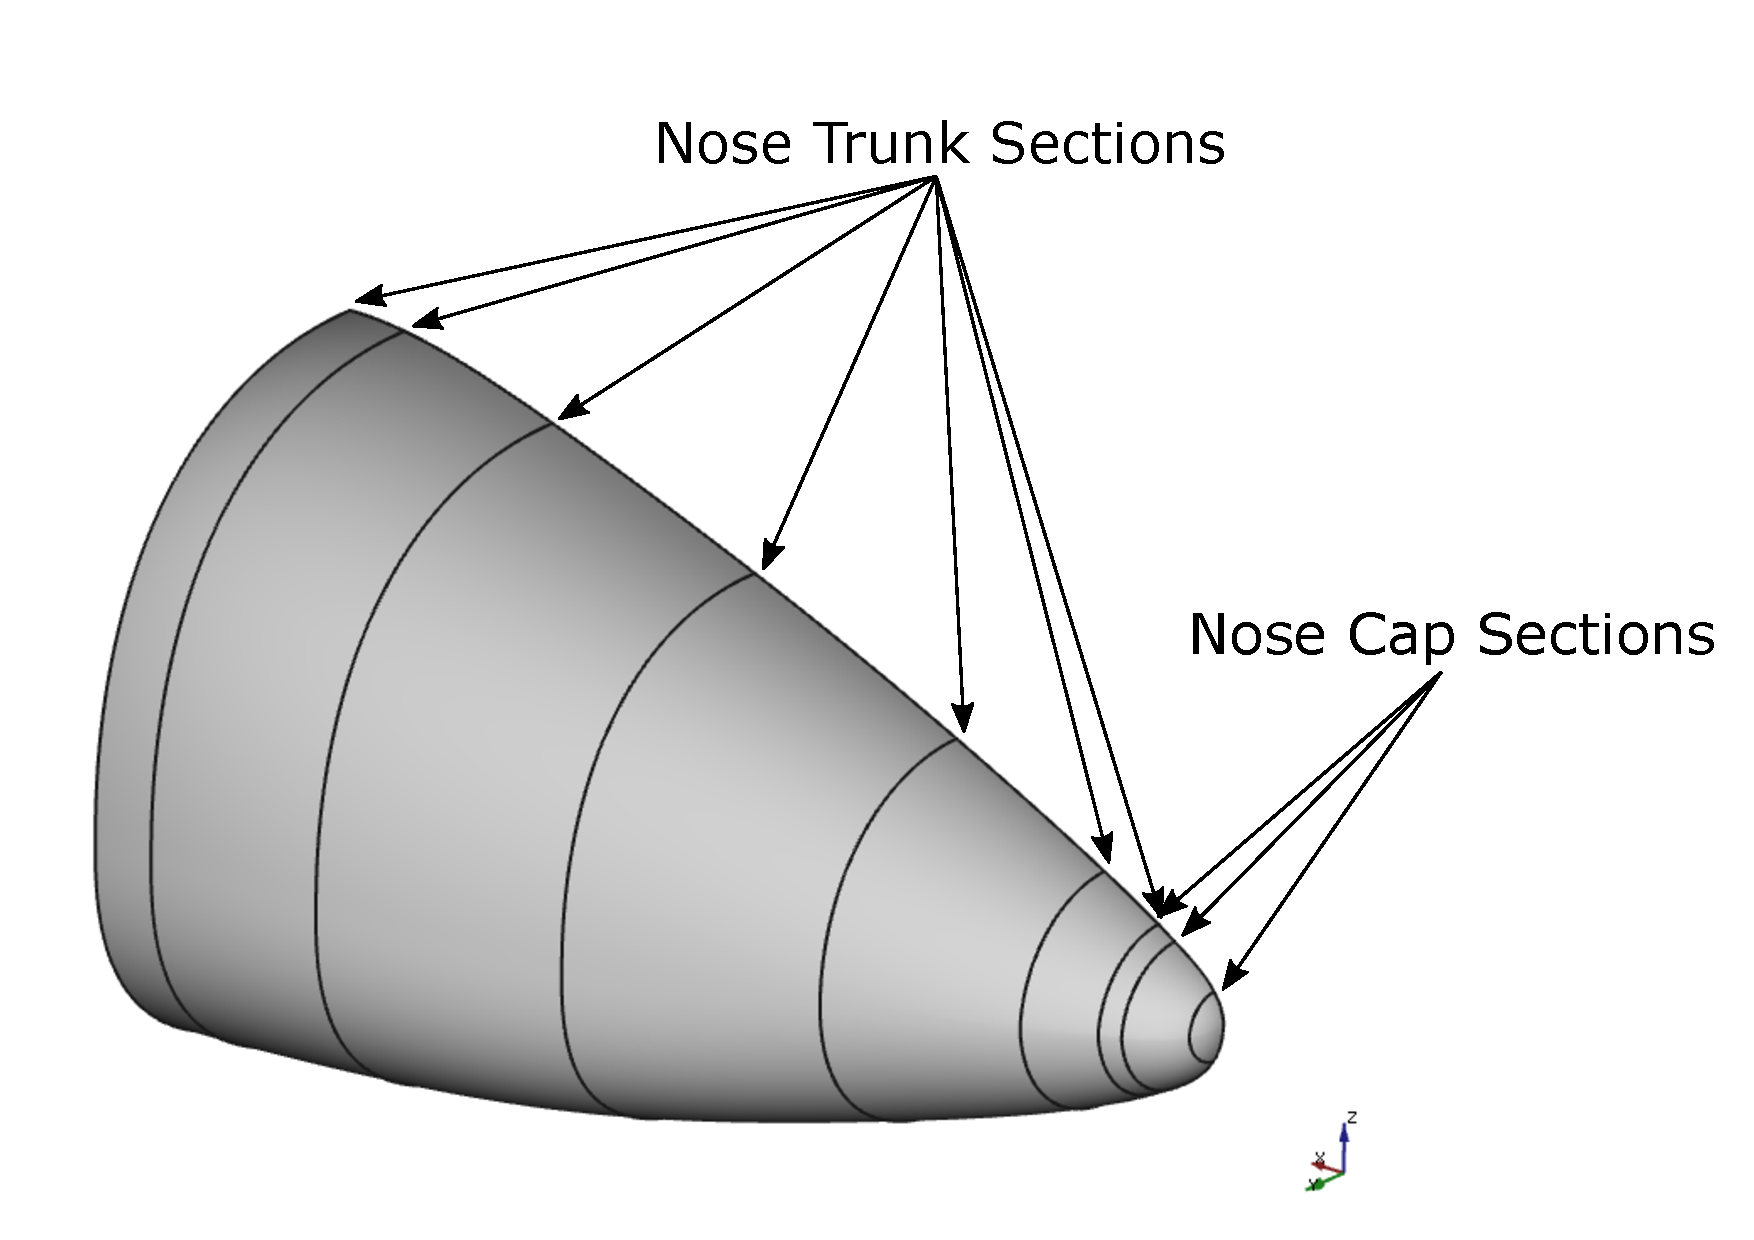
\includegraphics[scale=0.45]{Immagini/Capitolo3/nose_1}
\caption{Nose cap and nose trunk patches with supporting sections}
\label{fig:NoseCapPlusNoseTrunk}
\end{figure}
%

\bigskip
\noindent
The next step consists in generating the loft for the cylindrical section of the fuselage. This one is the easiest to obtain, since no particular attention must be paid to the number of supporting sections and the spacing between them. In fact, the \lstinline[language=Java]!getFuselageCAD! method doesn't even allow to choose the values for these parameters. Instead, the number of supporting sections is constantly set to three, with a linear spacing being used to separate them. The following lines of code describe the process through which cylindrical patch shapes have been built, with figure \ref{fig:FusCylinder} showing the result.
%
\bigskip
\begin{lstlisting}[caption={Fuselage cylinder building steps}, captionpos=b, tabsize=2, label={lst:FusCylinderCreation}]
// Determine the dimensional x-coordinates for the cylinder cross sections
List<Double> xmtPatch3 = Arrays.asList(
				MyArrayUtils.linspaceDouble(
						noseLength.doubleValue(SI.METER), 
						noseLength.plus(cylinderLength).doubleValue(SI.METER), 
						3)); // number of cross sections

// Generate supporting curves and make them available for export
List<CADGeomCurve3D> cadCrvCylinder = new ArrayList<>();
cadCrvCylinder.add(OCCUtils.theFactory.newCurve3DP(
		fuselage.getUniqueValuesYZSideRCurve(noseLength), false));				
cadCrvCylinder.add(OCCUtils.theFactory.newCurve3DP(
		fuselage.getUniqueValuesYZSideRCurve(
				noseLength.plus(cylinderLength.times(0.5))),false));				
cadCrvCylinder.add(OCCUtils.theFactory.newCurve3DP(
		fuselage.getUniqueValuesYZSideRCurve(
				noseLength.plus(cylinderLength)), false));
cadCrvCylinder.forEach(crv -> 
		extraShapes.add((OCCEdge) ((OCCGeomCurve3D) crv).edge()))	;				

// Generate the cylindrical loft by patching through the just created 3D curves.						
OCCShape patch3 = OCCUtils.makePatchThruSections(cadCrvCylinder);
\end{lstlisting}
%
\begin{figure}[H]
\centering
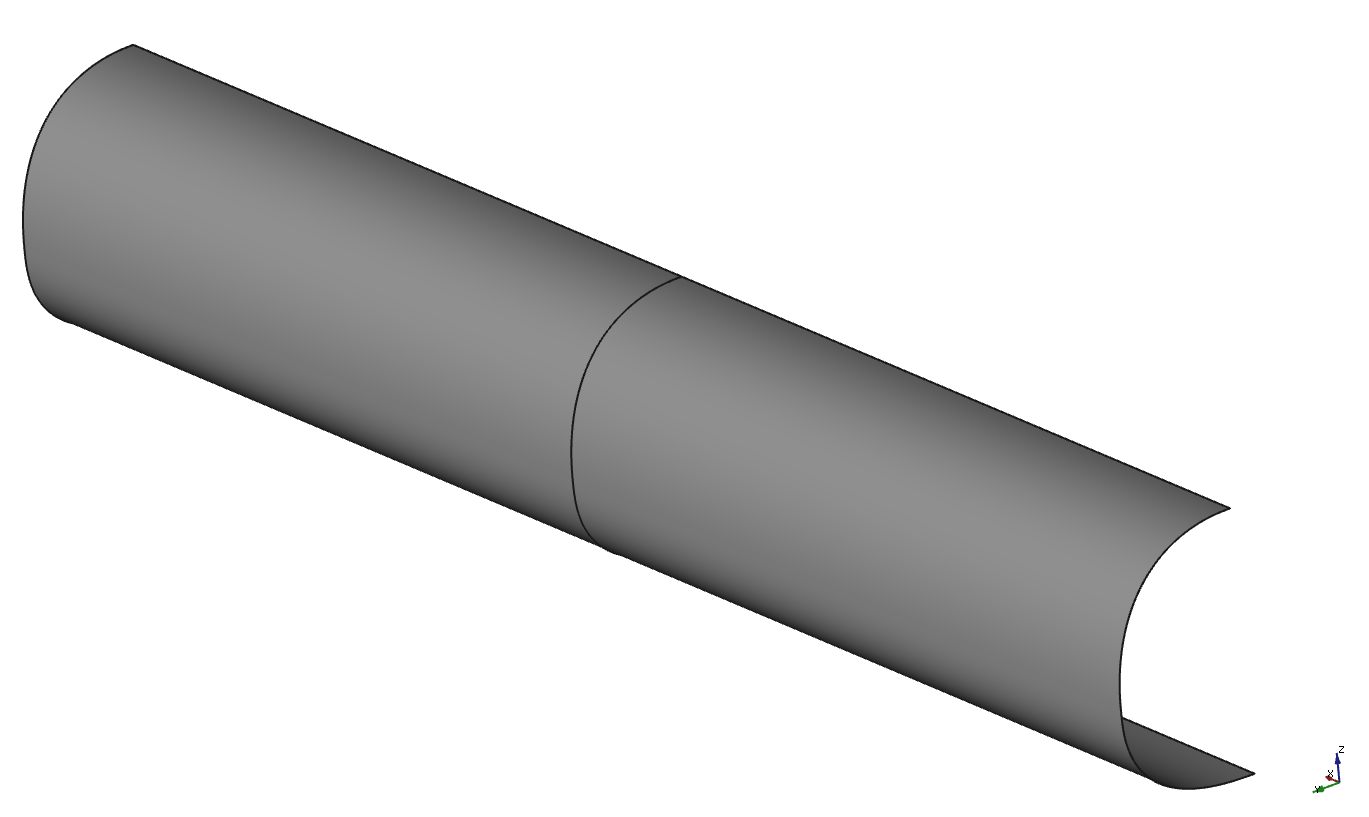
\includegraphics[scale=0.30]{Immagini/Capitolo3/FusCylinderPlusSupCurves}
\caption{Fuselage cylindrical section}
\label{fig:FusCylinder}
\end{figure}
%

\bigskip
\noindent
The generation of the tail shapes follows the same steps listed for the nose ones. The main difference consists in the different spacing adopted for the tail cap: in this case the half cosine spacing adopted forces an higher density towards the initial section of the list (so, in the negative $x$ direction). For the sake of completeness, the listing \ref{lst:TailCreation} reports part of the actual code used to generate tail shapes (including supporting sections), while figure \ref{fig:TailTrunkPlusTailCap} shows the just generated shape once being imported into a \gls{CAD} suite.
%
\bigskip
\begin{lstlisting}[caption={Tail trunk and cap building process}, captionpos=b, tabsize=2, label={lst:TailCreation}]
// Generate a list containing all tail trunk cross section x-coordinates
List<Double> xmtPatch4 = Arrays.asList(
				spacingTypeTailPatch.calculateSpacing(
						noseLength.plus(cylinderLength).doubleValue(SI.METER), 
						fuselageLength.minus(
								tailCapLength.times(tailCapSectionFactor1)).doubleValue(SI.METER), 
						numberTailPatchSections)
						);	

// Generate a list containing tail cap cross section x-coordinates				
List<Double> xmtPatch5 = Arrays.asList(
				MyArrayUtils.halfCosine1SpaceDouble(
						fuselageLength.minus(
								tailCapLength.times(tailCapSectionFactor1)).doubleValue(SI.METER), 
						fuselageLength.minus(
								tailCapLength.times(tailCapSectionFactor2)).doubleValue(SI.METER),
						numberTailCapSections) 
				);
		
// Generate tail trunk cross section curves and make them available for export.		
List<CADGeomCurve3D> cadCurvesTailTrunk = new ArrayList<>();
xmtPatch4.stream()
		.map(x -> Amount.valueOf(x, SI.METER))
		.forEach(x -> cadCurvesTailTrunk.add(
				OCCUtils.theFactory
						.newCurve3DP(fuselage.getUniqueValuesYZSideRCurve(x), false)
				));
						 
cadCurvesTailTrunk.stream()
		.map(crv -> (OCCEdge) ((OCCGeomCurve3D) crv).edge())
		.forEach(e -> extraShapes.add(e));	
		
// Generate tail cap cross section curves and make them available for export
CADVertex vertexTailTip = OCCUtils.theFactory.newVertex(
				fuselageLength.doubleValue(SI.METER), 0, zTailTip.doubleValue(SI.METER));
		
List<CADGeomCurve3D> cadCurvesTailCap = new ArrayList<>();
xmtPatch5.stream()
		.map(x -> Amount.valueOf(x, SI.METER))
		.forEach(x -> cadCurvesTailCap.add(
				OCCUtils.theFactory
						.newCurve3DP(fuselage.getUniqueValuesYZSideRCurve(x), false)
				));
						 
cadCurvesTailCap.stream()
		.map(crv -> (OCCEdge) ((OCCGeomCurve3D) crv).edge())
		.forEach(e -> extraShapes.add(e));	
		
// Generate the patch for the tail trunk
OCCShape patch4 = OCCUtils.makePatchThruSections(cadCurvesTailTrunk);


// Generate the patch for the tail cap
OCCShape patch5 = OCCUtils.makePatchThruSections(
		cadCurvesTailCapTrunk, vertexTailTip);
\end{lstlisting}
%

\bigskip
%
\begin{figure}[H]
\centering
\includegraphics[scale=0.40]{Immagini/Capitolo3/tail_1}
\caption{Tail cap and tail trunk patches with supporting sections}
\label{fig:TailTrunkPlusTailCap}
\end{figure}
%

\bigskip
\noindent
Once all the lofts have been created, they need to be sewed, in order to get one single shell. The \gls{OCCT} library provides the class to perform this kind of operation: it is called \lstinline[language=Java]!BRepBuilderAPI_Sewing! and provides methods in order to:
%
\begin{itemize}
\item create an empty builder,
\item add elements (generic shapes) to the builder,
\item set the tolerance,
\item compute the operation,
\item return the resulted shapes. 
\end{itemize}
%
The \lstinline[language=Java]!CADShapeFactory! actually contains methods in order to perform sewing operations, but starting from \lstinline[language=Java]!CADFace! instances. Since the shape we need to sew are actually shells, and sewing methods managing shell-type elements still need to be implemented in \lstinline[language=Java]!JPADCAD!, the actual code makes direct use of the \gls{OCCT} class. This is not the only case (as it will be clear in the next paragraphs and chapters), since \lstinline[language=Java]!JPADCAD! is still under constant development and testing. 
%
\bigskip
\begin{lstlisting}[caption={Lofts sewing process}, captionpos=b, tabsize=2, label={lst:PatchSewing}]
// Generate a new instance of the sewmaker class
BRepBuilderAPI_Sewing sewMaker = new BRepBuilderAPI_Sewing();

// Initalize the sewmaker and provide it with the patches.
// Finally, perform the sewing operation. 
sewMaker.Init();
sewMaker.Add(patch1.getShape());
sewMaker.Add(patch2.getShape());
sewMaker.Add(patch3.getShape());
sewMaker.Add(patch4.getShape());
sewMaker.Add(patch5.getShape());
sewMaker.Perform();

// Get the resulting TopoDS_Shape entity
TopoDS_Shape tds_shape = sewMaker.SewedShape();
\end{lstlisting}

\bigskip
\noindent
Once the sewing operation has been performed, the returned shape must be explored, in order to find shell-type entities. This operation is performed by means of the \lstinline[language=Java]!CADShapeFactory! method \lstinline[language=Java]!newExplorer!, which relies on the \lstinline[language=Java]!OCCExplorer! class constructors and allows to generate some sort of \emph{seeker} for desired shapes. This operation is fundamental, since the shape returned by the sewing algorithm belongs to the abstract \gls{OCCT} \lstinline[language=Java]!TopoDS_Shape! class.

\bigskip
\noindent
The next operation consists in mirroring the fuselage right shell obtained at the previous step. As mentioned in Chapter \ref{chap2}, the \gls{OCCT} library offers the possibility to perform basic geometry transformations. The class supervising this type of operation is called \lstinline[language=Java]!gp_Trsf!, which actually allows to perform:
%
\begin{itemize}
\item translation,
\item rotation,
\item scale,
\item reflection with respect to a point, a line, a plane.
\end{itemize}
%
The type of the operation can be choosed by means of several \lstinline[language=Java]!set! methods, that act directly on an empty instance of the \lstinline[language=Java]!gp_Trsf! class. In our case, a plane (the plane of symmetry of the fuselage) must be defined in order to perform the mirroring operation. The \gls{OCCT} class \lstinline[language=Java]!gp_Ax2! helps defining a plane by means of a point (the origin, expressed in terms of \lstinline[language=Java]!gp_Pnt!), and two directions (both expressend in terms of instances of the \gls{OCCT} class \lstinline[language=Java]!gp_Dir!), identifying the normal to the plane and a direction contained in the same plane. The following listing shows how the operation has been coded.
%
\bigskip
\begin{lstlisting}[caption={Fuselage right shell mirroring operations}, captionpos=b, tabsize=2, label={lst:ShellMirroring}]
// Define a new instance of the transformation class
gp_Trsf mirrorTransform = new gp_Trsf();

// Define the plane with respect to the shapes must be mirrored
gp_Ax2 mirrorPointPlane = new gp_Ax2(
		new gp_Pnt(0.0, 0.0, 0.0), // Origin
		new gp_Dir(0.0, 1.0, 0.0), // Y direction
		new gp_Dir(1.0, 0.0, 0.0)  // X direction
		);

// Select the the transformation to perform, add to it the just 
// created plane and generate a new instance of the actual OCCT
// class executing transformation on shape geometries
mirrorTransform.SetMirror(mirrorPointPlane);
BRepBuilderAPI_Transform mirrorBuilder = 
		new BRepBuilderAPI_Transform(mirrorTransform);
		
// Finally perform the mirroring operation
mirrorBuilder.Perform(sewedShell.getShape(), 1);
TopoDS_Shape mirroredShape = mirrorBuilder.Shape();
\end{lstlisting}

\bigskip
\noindent
In this case too it is necessary to go through the shapes produced by the mirroring operations in order to find shell-type entities. The operation performed is the same described above. Once the shells for the right and left side of the fuselage have been obtained, another sewing operation can be executed, returning one single shell, which will be the one to be used in order to create a solid entity. Altough the \lstinline[language=Java]!CADShapeFactory! contains methods generating solids, the ones currently implemented do not allow the production starting from shells. For this reason, at present, the code performs the creation of solid entities by using low level \gls{OCCT} classes. In particular, the class that implements this type of operation is called \lstinline[language=Java]!BRepBuilderAPI_MakeSolid! which provides methods for:
%
\begin{itemize}
\item defining and implementing the construction of a solid,
\item consulting the results.
\end{itemize}
%
Once the shell has been added to an empty instance of the solid builder class, the user just needs to use the \lstinline[language=Java]!Build! method in order to perform the construction. Figure \ref{fig:FusSolid} shows different views of the same solid fuselage, with the one depicted belonging to the ATR-72. 
%
\bigskip
\begin{lstlisting}[caption={Fuselage solid building step}, captionpos=b, tabsize=2, label={lst:FuselageSolid}]
// Generate a CADSolid empty instance 
CADSolid solidFuselage = null;

// Generate a new solidmaker empty object
BRepBuilderAPI_MakeSolid solidMaker = new BRepBuilderAPI_MakeSolid();

// Add the sewed halves of the fuselage to the solidmaker
// and perform the building operation
solidMaker.Add(TopoDS.ToShell(sewedShells.getShape()));
solidMaker.Build();

// Finally generate the fuselage CADSolid object by means of the
// OCCUtils newShape method, which accept a generic object of 
// the underlying implementation to build CAD-type ones
if(solidMaker.IsDone() == 1) {
		solidFuselage = (CADSolid) OCCUtils.theFactory.newShape(solidMaker.Solid());
}
\end{lstlisting}

\bigskip
\noindent
The \lstinline[language=Java]!getFuselageCAD! method implemented in \lstinline[language=Java]!AircraftUtils! allows not only to export the final solid shape of the fuselage. It also gives the user the possibility to choose between which types of shape he wants to export and write to file. For example, by setting to \lstinline[language=Java]!true! the \lstinline[language=Java]!exportSupportShapes! parameter and \lstinline[language=Java]!false! the remaining ones, just the wireframe of the fuselage would be exported. For sake of completeness, figure \ref{fig:FusWireframe} shows the wireframe (completed by the outline curves, whose calculation is performed by the code but not actually used for loft generation purposes) of the fuselage of the ATR-72.

\bigskip
%
\begin{figure}[H]
\centering
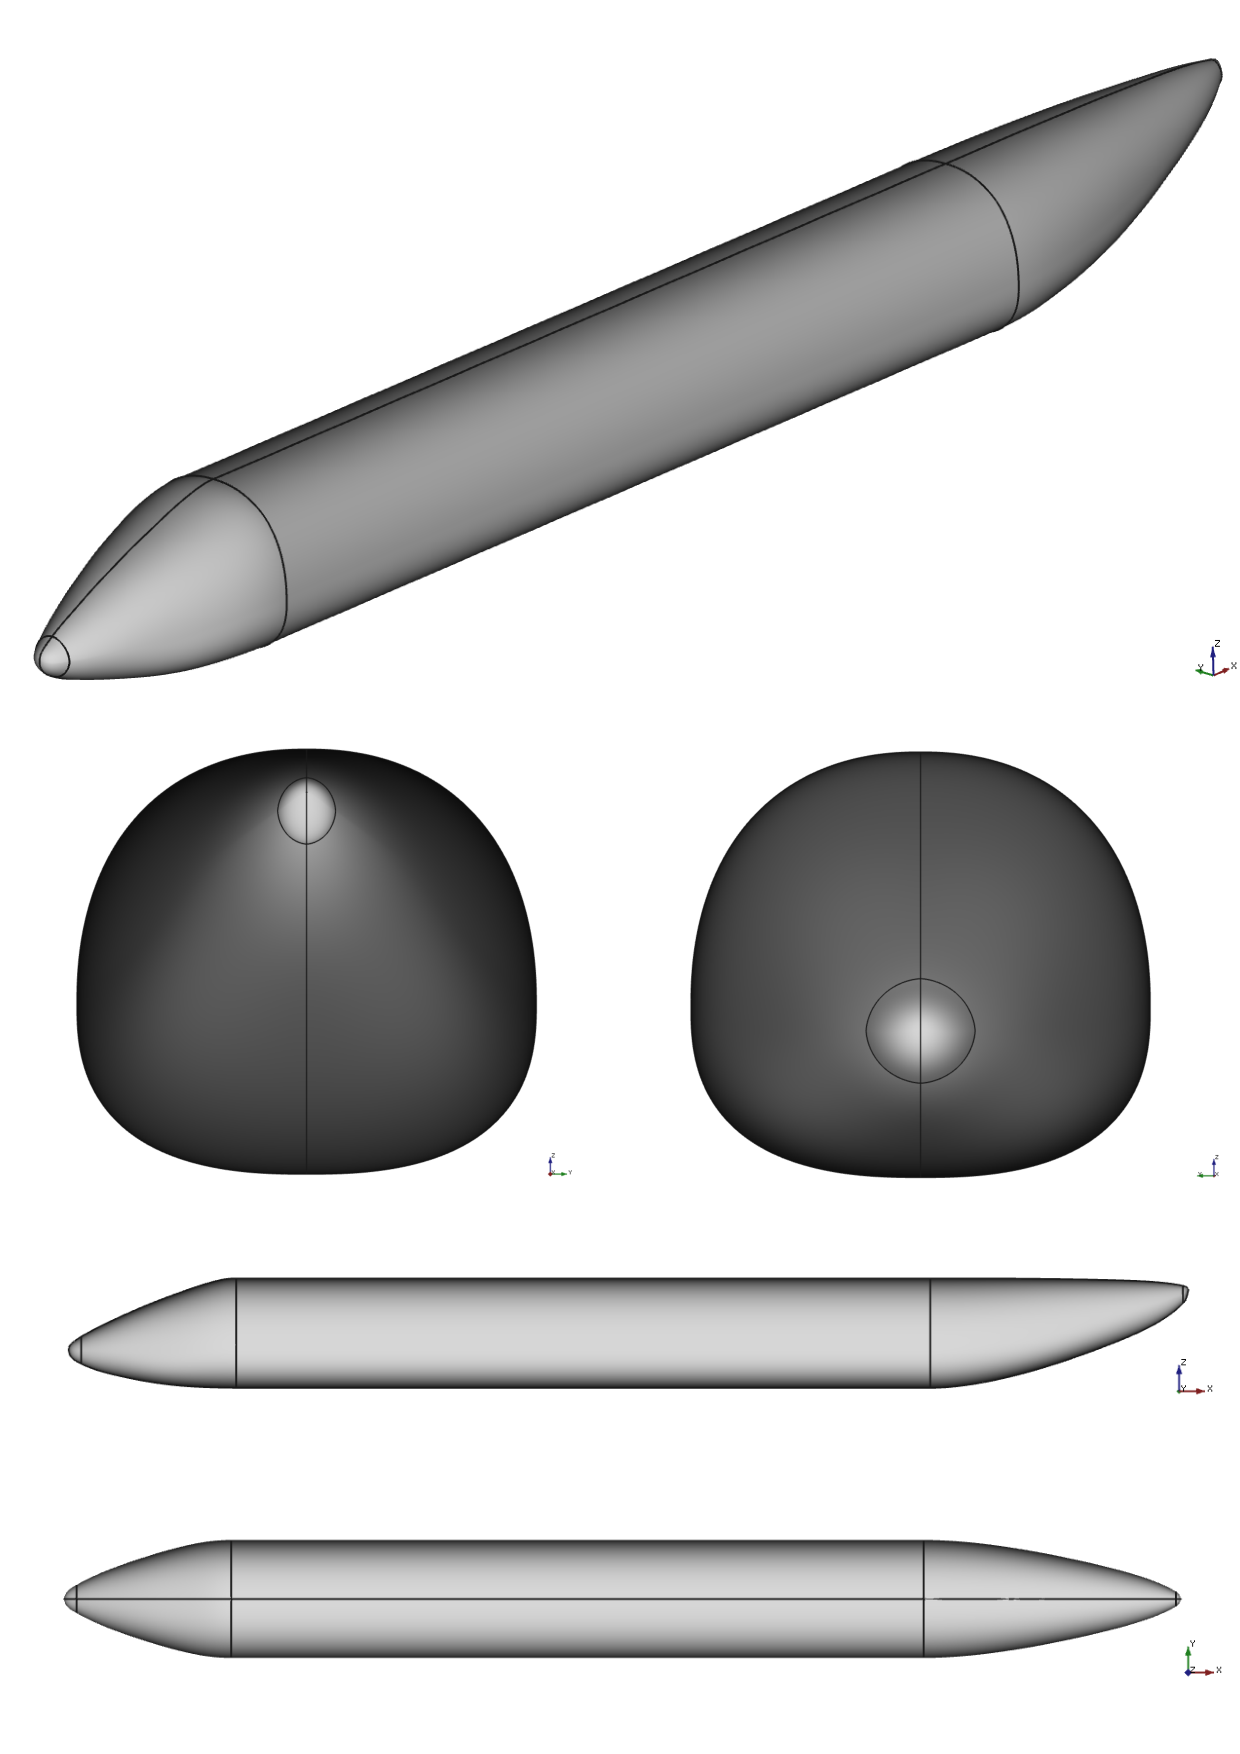
\includegraphics[scale=0.45]{Immagini/Capitolo3/fussolid_1}
\caption{ATR-72 solid fuselage, different views}
\label{fig:FusSolid}
\end{figure}
%
\begin{figure}[H]
\centering
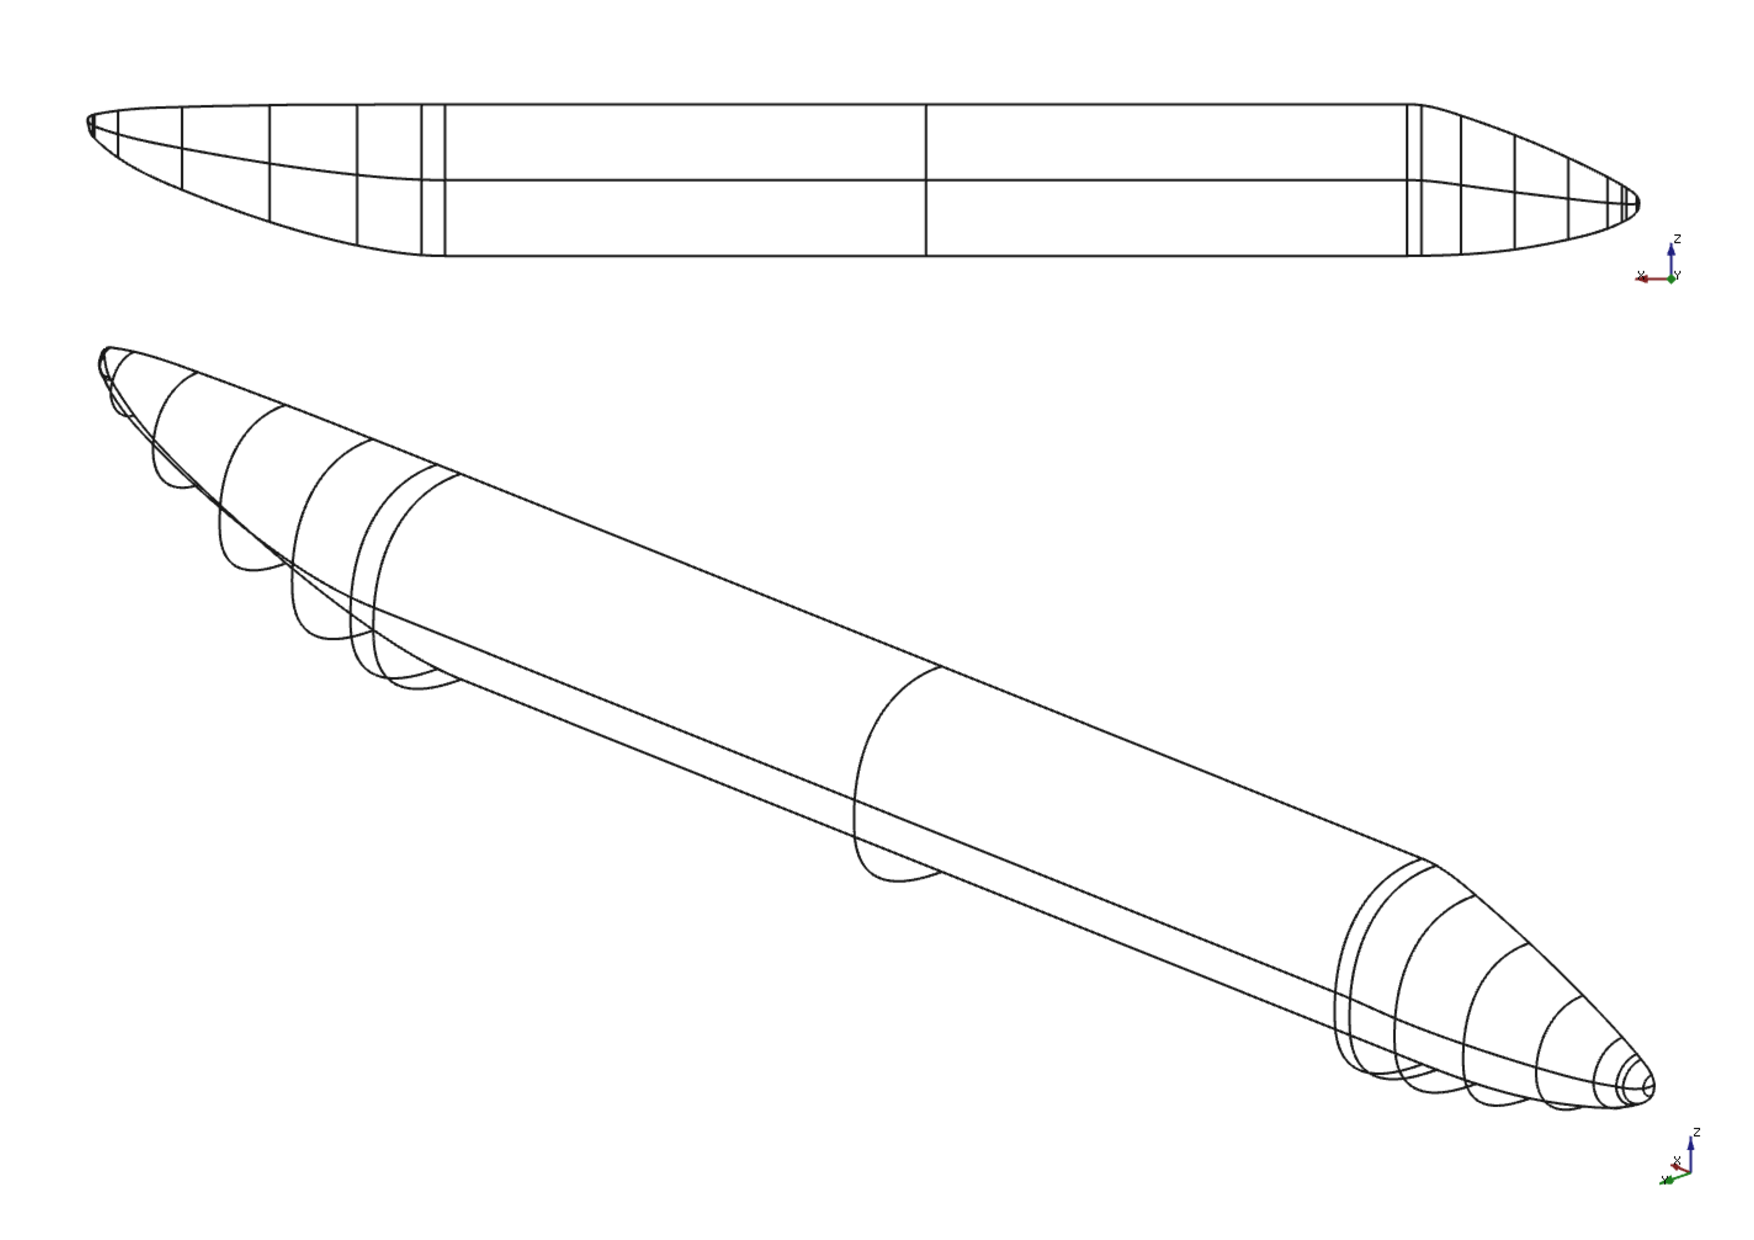
\includegraphics[scale=0.32]{Immagini/Capitolo3/fuswireframe_1}
\caption{ATR-72 fuselage wireframe, different views}
\label{fig:FusWireframe}
\end{figure}

\section{Lifting surface CAD method}
\label{sec3.4}

The construction of the shapes representing a generic lifting surface revolves around three main stages, tipically:
%
\begin{enumerate}
\item generate one loft for each panel of the wing;
\item generate a shell for the tip of the wing;
\item reflect the resulting shapes with respect to a symmetry plane (whether necessary).
\end{enumerate}
%
\begin{figure}[H]
\centering
\includegraphics[scale=0.47]{Immagini/Capitolo3/wing_1}
\caption{Wing patches for a JPAD wing}
\label{fig:WingPatches}
\end{figure}
%
The \lstinline[language=Java]!AircraftUtils! method that provides for the construction of lifting surfaces is called \lstinline[language=Java]!getLiftingSurfaceCAD!. This method accepts the following inputs.
%
\begin{itemize} 
\renewcommand\labelitemi{\tiny$\blacksquare$}
\renewcommand\labelitemii{\tiny$\bullet$}
\item \textbf{\lstinline[language=Java]!liftingSurface!} - An instance of the JPAD \lstinline[language=Java]!LiftingSurface! class, that is used in order to describe and collect geometric, aerodynamic and mass characteristics of a generic lifting surface. It provides also the methods to access all these information.
\item \textbf{\lstinline[language=Java]!typeLS!} - An instance of the JPAD \lstinline[language=Java]!ComponentEnum! class, which provides support for aircraft components enumeration. The \lstinline[language=Java]!getLiftingSurfaceCAD! algorithm makes use of this argument in order to distinguish between different typologies of lifting surfaces. It is necessary for the code to know with which kind of surface it is dealing with, in order to perform the necessary checks and to activate the right flags for certain types of operations.
\item \textbf{\lstinline[language=Java]!tipTolerance!} - A \lstinline[language=Java]!double! entry fixing the tolerance for the process of sewing the tip of the lifting surface (which is modeled separately) with the rest of the wing.
\item \textbf{\lstinline[language=Java]!exportLofts!, \lstinline[language=Java]!exportSolid!, \lstinline[language=Java]!exportSupportShapes!} - Entries of the \lstinline[language=Java]!boolean! type, that allow to export, respectively, the shells (wing and tip), the solid, and the wireframe of the lifting surface.
\end{itemize}
%
\noindent
First things the algorithm executes regard data collection (by means of the methods provided by the \lstinline[language=Java]!LiftingSurface! class) and the wing wireframe construction. One of the datum that must be collected is the one related to the number of panels that constitute the wing. This number is tipically equal to two for proper wings, one for the other lifting surfaces such as the tail ones and the canard. Once all the necessary data has been collected, the construction of the wireframe of the wing can begin. For this purpose, leading edge, trailing edge, and airfoil curves must be created. It has to be noted that, as for the fuselage construction, some of the wireframe shapes generated are not intended to be used for lofting operations. Leading and trailing edge segments, for example, just serve for graphical purposes, and are not actually used as guide curves when performing patching. Furthermore, being generated by means of just two points (obtained by wing breakpoints coordinates), these edges are just segments and do not follow the actual profile of the curves they are meant to represent. On the contrary, airfoil curves are actually used to generate lofts, by patching through them using the same algorithms described in the previous paragraph and in Chapter \ref{chap2}. The \lstinline[language=Java]!liftingSurface! object passed to the method allows access to the list of airfoils located at the wing breakpoints. This list contains objects of the \lstinline[language=Java]!Airfoil! type, which is the class that in \gls{JPAD} manages aerodynamic and geometric characteristics of airfoils, and provides methods that give access to the $x$ and $z$ coordinates of its points. Since these points just define the \emph{absolute} airfoil (the airfoil with its chord aligned with the $x$ axis and length equal to $1$), they need to be modified in order to correctly represent the actual airfoils at some precise locations along the lifting surface. The \lstinline[language=Java]!AircraftUtils! class has then been provided with a private method called \lstinline[language=Java]!populateCoordinateList!. This method receives:
%
\begin{itemize}
\item a \lstinline[language=Java]!double! representing the $y$ station at which the airfoil points must be calculated;
\item an object of the \lstinline[language=Java]!Airfoil! class, which provides the basic airfoil points;
\item an object of the \lstinline[language=Java]!LiftingSurface! type, that provides wing characteristics (in terms of chord length, twist angle, and leading edge coordinates) at precise locations along its span;
\end{itemize}
and returns a \gls{List} of \lstinline[language=Java]!double[]! points, representing the actual coordinates of the airfoil. This method also performs several checks on the points it is supplied to. A first check is made on the points imported from the \lstinline[language=Java]!Airfoil! object by controling there are no duplicates among the list, in order to avoid problems once the spline interpolation needs to be performed. Another check is made on the trailing edge of the airfoil, which has to be opened in case the $z$ coordinates of the first and last points of the list coincide. This is a necessary operation, especially when the import of the \gls{CAD} model of the wing into a \gls{CFD} suite is something planned. Currently the method does not allow to adjust the value of the gap between the points: the code automatically opens the trailing edge if the distance between the first and the last point of the basic airfoil is less than $10^{-5}\si{\meter}$ in the $z$ direction, setting it to $10^{-4}\si{\meter}$.
%
\bigskip
\begin{lstlisting}[caption={Opening creation at the trailing edge}, captionpos=b, tabsize=2, label={lst:OpeningTE}]
if(Math.abs(zCoords[0] - zCoords[nPoints - 1]) < 1e-5) {
			zCoords[0] += 5e-4;
			zCoords[nPoints - 1] -= 5e-4;
		}
\end{lstlisting}

\bigskip
\noindent
Once the points have been obtained, they can be interpolated by means of one of the factory methods for 3D curves seen in Chapter \ref{chap2}. These methods interpolate a list of points by using a \gls{acr:NURBS} curve and provide a \lstinline[language=Java]!CADGeomCurve3D! object representing the curve itself. Figure \ref{fig:AirfoilSample} shows an example of an airfoil obtained by applying the aforementioned methods. In particular, the figure depicts a NACA 23018 airfoil.
%
\begin{figure}[H]
\centering
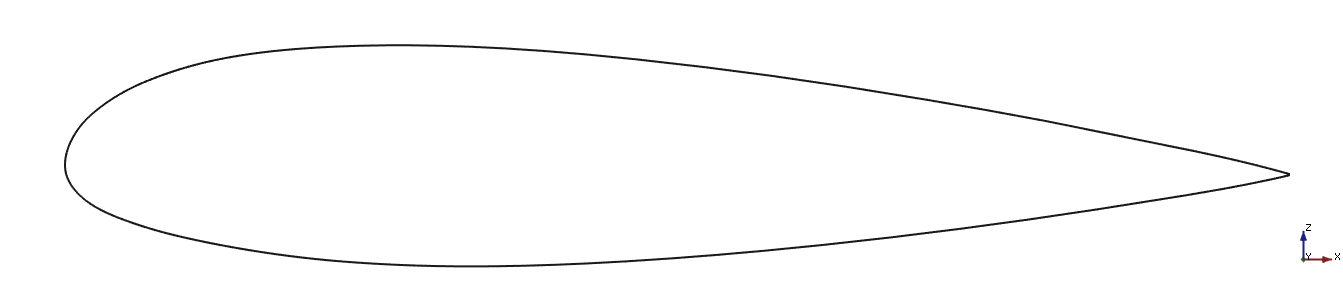
\includegraphics[scale=0.28]{Immagini/Capitolo3/WingAirfoil}
\caption{NACA 23018 airfoil curve generated in JPAD}
\label{fig:AirfoilSample}
\end{figure}
%
\noindent
The method described above allows to build airfoils at every desired location along the wing span. A first group of airfoils is generated at the breakpoints, while secondary groups are created between them. The reason behind having multiple airfoils between breakpoint ones resides in the necessity to create wing lofts, one for each panel, by patching through more than just two airfoil curves at a time, in order to reduce the risk of having unexpected results and to increase final shapes adherence to real counterparts. Since the number of panels is not something that can be known \emph{a priori} when applying \gls{CAD} generating methods for lifting surfaces, the user is not currently enabled to fix the number of cross sections for each patch. However, the code automatically sets it, based on the length of each panel respet to the total wing span. At the end of this process, a list of lists of \lstinline[language=Java]!CADGeomCurve3D! is filled, with each of the sub-lists associated to a specific panel. Figure \ref{fig:WingWireframe} shows the wireframe created to this point, with breakpoints airfoils also provided with their chord segment.
%
\begin{figure}[H]
\centering
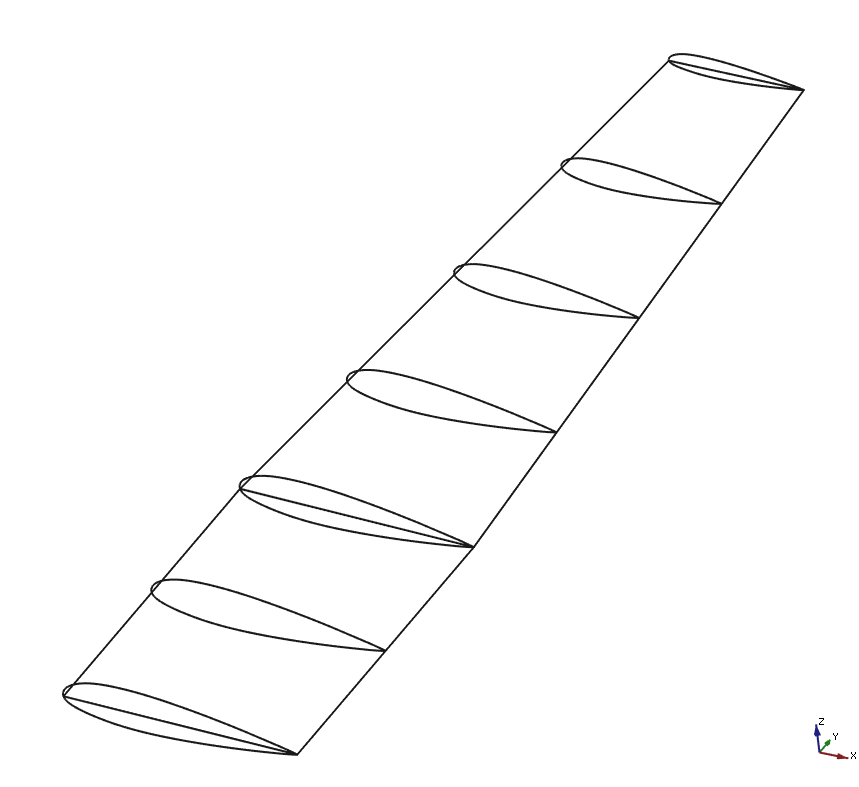
\includegraphics[scale=0.42]{Immagini/Capitolo3/WingWireframe}
\caption{Wing wireframe, with no sketching curves for the tip}
\label{fig:WingWireframe}
\end{figure}
% 

\bigskip
\noindent
As mentioned before, the \lstinline[language=Java]!getLiftingSurfaceCAD! method also generates shapes for the wing tip. These shapes are created by following the same steps used for the construction of fuselage and wing patches. The main difference in this case consists in the fact that the curves to patch through needs to be created from scratch, since \gls{JPAD} \lstinline[language=Java]!LiftingSurface! class does not contain a description for the tip. The very first operation consists in splitting the tip and penultimate airfoils (i.e., the last and the second-to-last of the airfoils depicted in figure \ref{fig:WingWireframe}) in two halves at their leading edge, by means of the wing wireframe generated at the previous step. These operations are necessary for two reasons:
%
\begin{itemize}
\item allow to better shape the leading edge of the wing tip by splitting its filling process in two steps, one regarding the upper side and one regarding the lower one;
\item the algorithm that has been implemented in order to generate the cross sections for the wing tip necessitates both the upper and the lower side curves of the tip and pre-tip (penultimate) airfoils. 
\end{itemize}
%
Besides, since it is quite likely that the leading edge of the tip airfoil does not precisely pass through the points of the leading edge of the wing wireframe, a further manipulation is necessary. This operation consists in forcing the two halves of the tip airfoil to pass through the last of the points describing the leading edge wireframe, and, in order to make sure the two halves preserve their original shape as much as possible, a much larger number of points is used to discretize them. This operation is quite necessary, since in case the condition described above is not satisfied the filling operations for the wing tip leading edge could encounter some problematics while are executed. 

\bigskip
\noindent
In order to build the necessary supporting curves for the tip shell, some construction must be performed first. For one thing, some sort of supporting plane is built, by simply extending the leading and trailing edge segments of the wing wireframe in the positive $y$ direction. The amount of this extension is related to the thickness of the tip airfoil. This extension generates the points A and B (figure \ref{fig:WingTip1}), and the segments a, b, and c, that define the actual construction plane for the wing tip. These operations are performed by means of \lstinline[language=Java]!PVector! objects, that prove to be really useful especially when managing directions and point definitions. In order to obtain an authentic plane at the previous step, point B $z$ coordinate is slightly changed and adjusted (whether the lifting surface being built is not a vertical tail) in order to make it coincide with the one of point A. Once the construction plane has been obtained, it is possible to build the first of the supporting curves for the tip. The points for this curve are obtained by using the \lstinline[language=Java]!PVector! class too, which provides static methods to perform linear interpolation between one vector and another. In particular, the point C is the point at the $25\%$ of the segment b (that has been oriented from A to B, so in the positive $x$ direction), while the point D is at the $75\%$ of the same segment. Point E is at the $75\%$ of the segment connecting the leading and trailing edge of the tip airfoil, while F is at the $90\%$ of the edge that connects the points D and E. Finally, point G is obtained as the point at the $25\%$ of the segment c. 
%
\bigskip
\begin{lstlisting}[caption={Points for the in-plane tip construction curve}, captionpos=b, tabsize=2, label={lst:ConstCurvePnts}]
double[] mainVSecVector = {0.25, 0.75};
PVector cPnt = PVector.lerp(aPnt, bPnt, (float) mainVSecVector[0]);
PVector dPnt = PVector.lerp(aPnt, bPnt, (float) mainVSecVector[1]);	
PVector ePnt = PVector.lerp(le2, te2, (float) mainVSecVector[1]);
PVector fPnt = PVector.lerp(ePnt, dPnt, 0.90f);	
PVector gPnt = PVector.lerp(bPnt, te2, 0.25f);
\end{lstlisting}

\bigskip
\noindent
In order to shape the in-plane construction curve correctly, tangent vectors must be assigned. In particular, the curve is assigned three tangency constraints: one in A, one in C, and the last one in G. These tangent vectors are obtained by means of several \lstinline[language=Java]!PVector! entities manipulations. Since the \gls{OCCT} algorithm underlying the \lstinline[language=Java]!newCurve3D! factory methods allow to assign tangency constraints only at the initial and final points of a curve, two in-plane construction curves are actually built, with the second one being split (at the point F) by means of the \lstinline[language=Java]!OCCUtils.splitEdge! method, in order to facilitate the subsequent necessary manipulations (listing \ref{lst:ConstrCurves}).
%
\bigskip
\begin{lstlisting}[caption={In-plane construction curves building steps}, captionpos=b, tabsize=2, label={lst:ConstrCurves}]
// Point lists for the in-plane construction curves
List<double[]> constrPlaneGuideCrv1Pnts = new ArrayList<>();
constrPlaneGuideCrv1Pnts.add(new double[] {le2.x, le2.y, le2.z});
constrPlaneGuideCrv1Pnts.add(new double[] {cPnt.x, cPnt.y, cPnt.z});
		
List<double[]> constrPlaneGuideCrv2Pnts = new ArrayList<>();
constrPlaneGuideCrv2Pnts.add(new double[] {cPnt.x, cPnt.y, cPnt.z});
constrPlaneGuideCrv2Pnts.add(new double[] {fPnt.x, fPnt.y, fPnt.z});
constrPlaneGuideCrv2Pnts.add(new double[] {gPnt.x, gPnt.y, gPnt.z});

// Generate tangent vectors
PVector leVector = PVector.sub(le2, le1); // Vector representing the LE segment
PVector aVector = PVector.mult(leVector, aLength);
PVector cVector = PVector.sub(cPnt, aPnt); 
PVector gVector = PVector.sub(gPnt, fPnt);

// Weights for the tangency constraints
double tanAFac = 1;
double tanCFac = (cVector.mag()/aVector.mag())*0.75;
double tanGFac = tanCFac;

// Tangent vectors normalization
aVector.normalize();
cVector.normalize();
gVector.normalize();	
		
// Actual tangent vectors for the construction curves.
double[] tanAConstrPlaneGuideCrv = MyArrayUtils.scaleArray(
		new double[] {aVector.x, aVector.y, aVector.z}, tanAFac);
double[] tanCConstrPlaneGuideCrv = MyArrayUtils.scaleArray(
		new double[] {cVector.x, cVector.y, cVector.z}, tanCFac);
double[] tanGConstrPlaneGuideCrv = MyArrayUtils.scaleArray(
		new double[] {gVector.x, gVector.y, gVector.z}, tanGFac);

// Points interpolation
CADGeomCurve3D constrPlaneGuideCrv1 = OCCUtils.theFactory.newCurve3D(
				constrPlaneGuideCrv1Pnts, 
				false, 
				tanAConstrPlaneGuideCrv, 
				tanCConstrPlaneGuideCrv, 
				false);					
CADGeomCurve3D constrPlaneGuideCrv2_0 = OCCUtils.theFactory.newCurve3D(
				constrPlaneGuideCrv2Pnts, 
				false, 
				tanCConstrPlaneGuideCrv, 
				tanGConstrPlaneGuideCrv, 
				false);
								
// Split constrPlaneGuideCrv2_0 for further manipulations
List<OCCEdge> constrPlaneGuideCrvs2 = OCCUtils.splitEdge(
		constrPlaneGuideCrv2_0, 
		new double[] {fPnt.x, fPnt.y, fPnt.z});		
		
CADGeomCurve3D constrPlaneGuideCrv2 = 
		OCCUtils.theFactory.newCurve3D(constrPlaneGuideCrvs2.get(0));
CADGeomCurve3D constrPlaneGuideCrv3 = 
		OCCUtils.theFactory.newCurve3D(constrPlaneGuideCrvs2.get(1));
\end{lstlisting}
%
\begin{figure}[H]
\centering
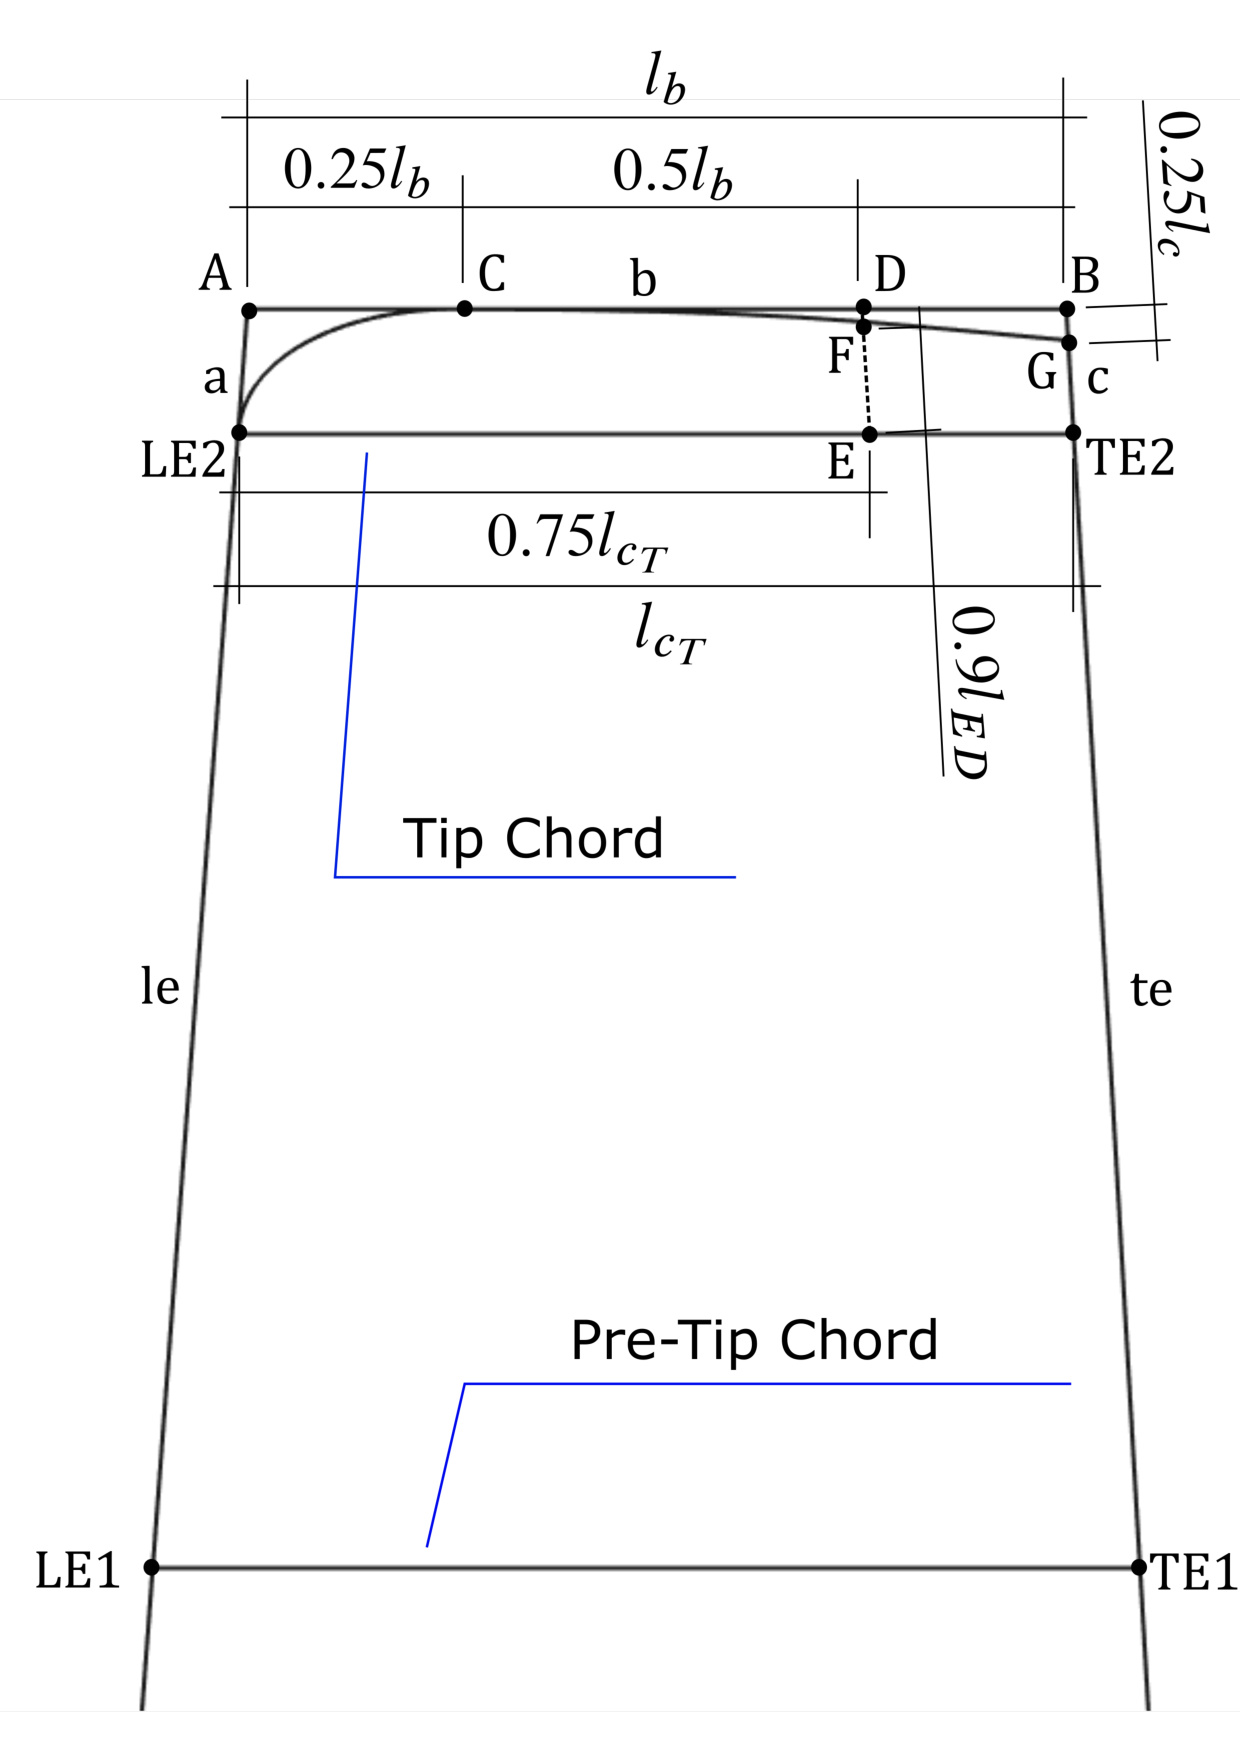
\includegraphics[scale=0.42]{Immagini/Capitolo3/wingtip_1}
\caption{Wing tip construction plane, complete with point definitions and edge dimensions}
\label{fig:WingTip1}
\end{figure}
% 
\begin{figure}[H]
\centering
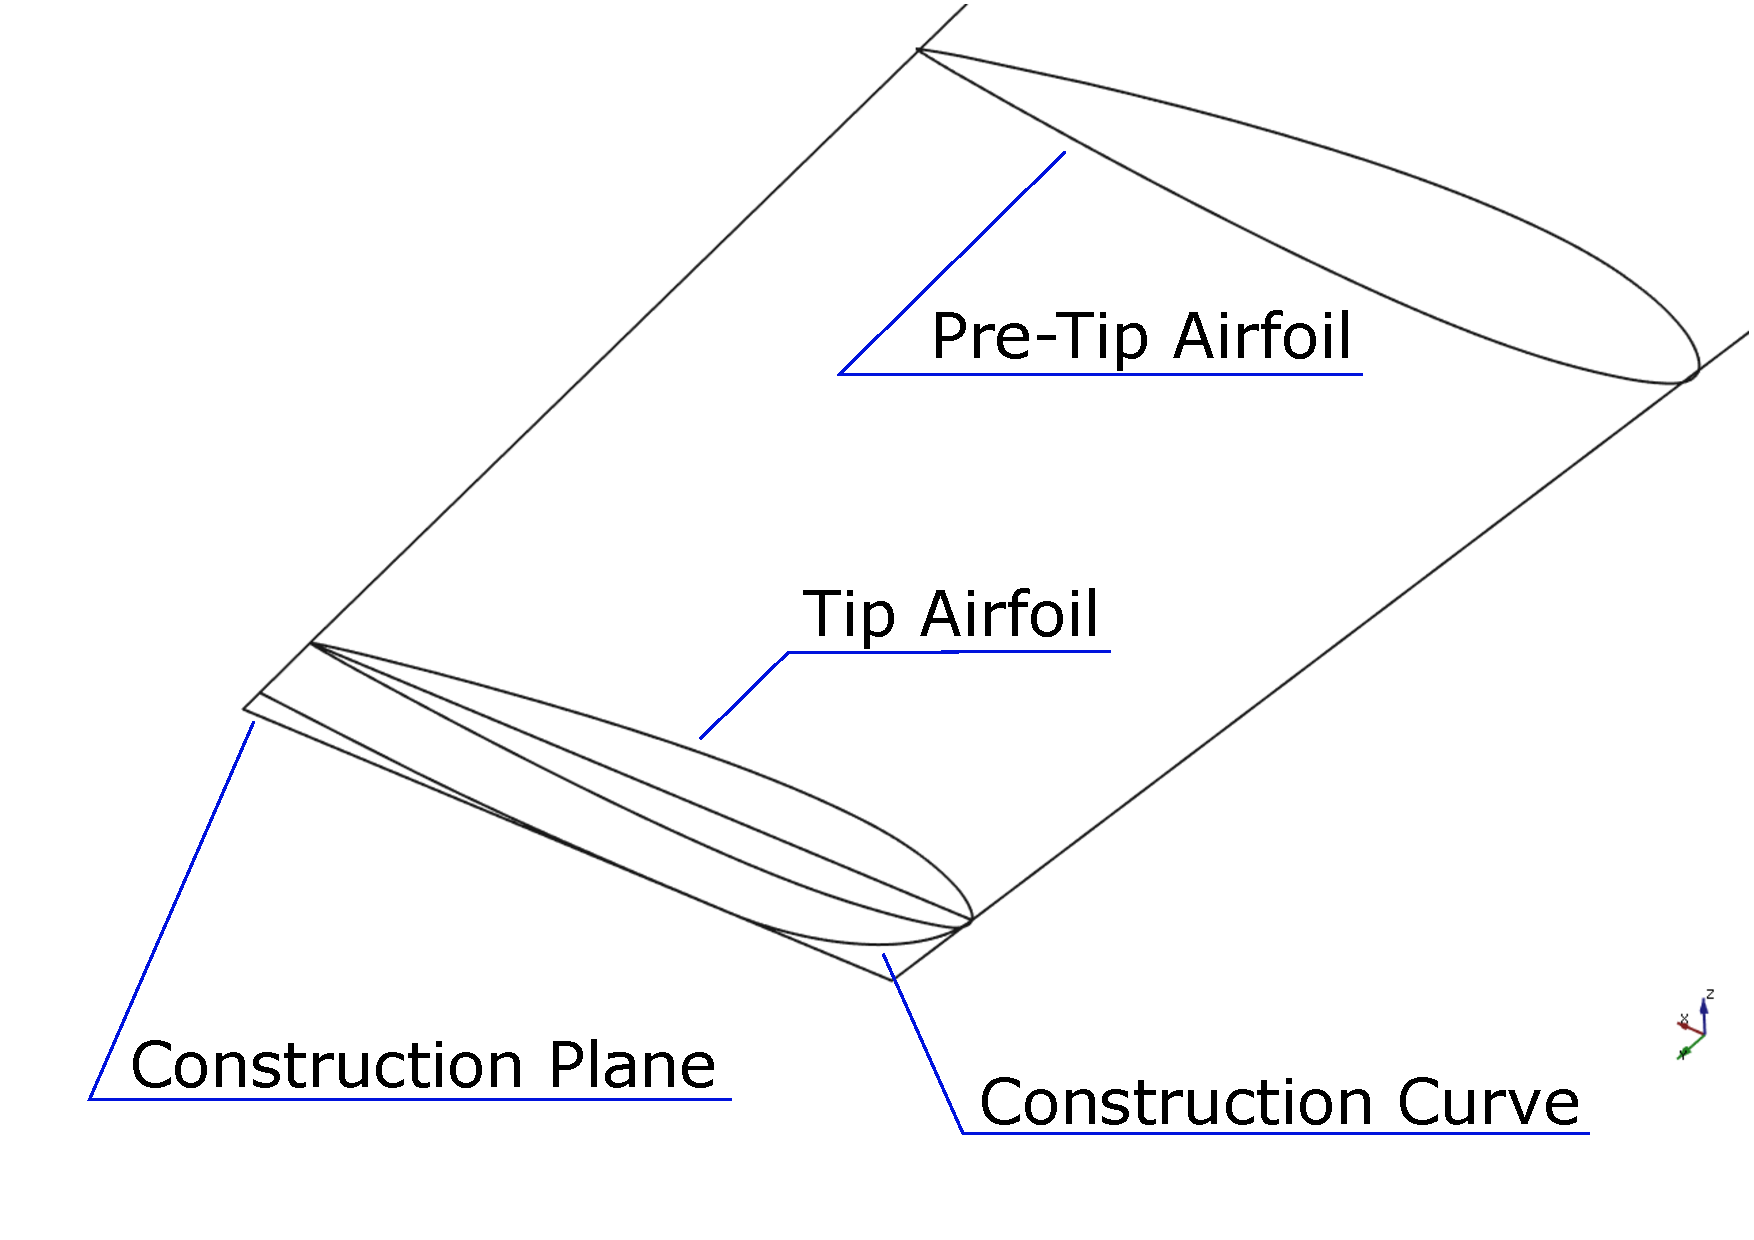
\includegraphics[scale=0.37]{Immagini/Capitolo3/wingtip_2}
\caption{Wing tip in-plane construction curve}
\label{fig:WingTip1}
\end{figure}
% 

\bigskip
\noindent
The in-plane construction curves serve as some sort of guide for the actual supporting curves of the wing tip, by providing points for their construction. First cross section curves to be generated are those passing for the points C, F, and G. \lstinline[language=Java]!AircraftUtils! contains a private static method, called \lstinline[language=Java]!createVerCrvsForTipClosure!, that generates cross section curves for the tip (in the form of \lstinline[language=Java]!CADGeomCurve3D! objects) by means of the following arguments:
%
\begin{itemize}
\item an instance of the \lstinline[language=Java]!LiftingSurface! class representing the lifting surface;
\item two Java \gls{List}s of \lstinline[language=Java]!OCCEdge! objects, containing respectively the upper and the lower edges of the tip and pre-tip airfoil;
\item two \lstinline[language=Java]!PVector! entities, representing the directions of the leading and trailing edge of the wing wireframe, respectively;
\item a \lstinline[language=Java]!double! entry, whose value is between $0.0$ and $1.0$, and states at which station, in terms of the tip chord fraction, the supporting curve needs to be created;
\item 3D point coordinates in the form of a \lstinline[language=Java]!double! array, representing the point on the in-plane construction curve that the supporting curve needs to pass through.
\end{itemize}
%
This algorithm uses the entries listed above in order to build curves that start on the upper side of the wing tip airfoil and end on the lower one, passing through the in-plane construction curve. In order to get the necessary points on the tip airfoil curves, the method makes use of the \lstinline[language=Java]!PVector! \lstinline[language=Java]!cross! static function, which allows to calculate the cross product between vectors. The cross product one is interested in in this case is the one between the vector representing the chord (or a fraction of it) of the wing tip airfoil and one of the vectors belonging to the construction plane (such as the leading and trailing edge vectors passed to the method), in order to generate segments belonging to the tip airfoil plane and perpendicular to its chord. These segments are then used to calculate points on the airfoil curves, once being multiplied by a scalar quantity representing the semi-airfoil (upper or lower side) height with respect to its chord. These scalar quantities are provided by a private static method, still contained in \lstinline[language=Java]!AircraftUtils! and called \lstinline[language=Java]!getThicknessAtX!, which requires an object belonging to the \gls{JPAD} \lstinline[language=Java]!Airfoil! class (representing the basic airfoil) and a \lstinline[language=Java]!double! value standing for the chord fraction at which the heights (both in the up and down direction) of the airfoil curve must be calculated. The segments, once scaled, finally provide the points on the airfoil curve, by means of the static method \lstinline[language=Java]!pointProjectionOnCurve! contained in \lstinline[language=Java]!OCCUtils!. 

\bigskip
\noindent
Points are not the only thing needed in order to generate the cross section curves of the wing tip. Three tangency constraints need to be imposed onto these curves: one at the starting point, on the upper side of the tip profile; the second one at the intersection with the in-plane curve; the last one at the ending point, on the lower side of the tip curve. These tangency constraints (the first and the last one in particular) are calculated still by means of the curves of the last and penultimate airfoils. In fact, in order to obtain a smooth transition from the last panel shell to the one of the wing tip, tangent vectors are calculated by simply connecting corresponding points (i.e., points located at the same chord fraction) onto the penultimate and last airfoil. Points on the pre-tip airfoil curve are calculated in the same way as described above. Regarding the second tangent vector, instead, it is simply imposed coincident with the normal vector of the wing tip construction plane. In order to obtain the right shape for the supporting curves, tangent vector magnitudes are adjusted according to some parameters, which depend on the tip airfoil thickness and on the distance between the in-plane construction curve and tip airfoil plane at the cross section at which the curve is being calculated. The piece of code below (listing \ref{lst:TipSupCurves}) just gives a glimpse at the operations behind the search of the appropiate magnitudes for the tangent vectors. Once all these operations are accomplished, the algorithm finally performs the curves calculation. For the same reasons specified above, the code produces two supporting curves at a time, that are collected into a \lstinline[language=Java]!CADGeomCurve3D! array and returned to the calling method. Figure \ref{fig:WingTip1} shows the result obtained at this stage.
%
\bigskip
\begin{lstlisting}[caption={Tip supporting curves tangent vectors magnitudes}, captionpos=b, tabsize=2, label={lst:TipSupCurves}]
// Determine tip airfoil thicknesses with respect to its chord segment
double thickUpp = PVector.sub(pntOnTipAirfoilUCrv, pntOnTipChord).mag();
double thickLow = PVector.sub(pntOnTipAirfoilLCrv, pntOnTipChord).mag();

// Determine construction curve height with respect to
// the tip airfoil chord segment
double crvHeight = PVector.sub(
		new PVector(
				(float) guideCrvPnt[0], 
				(float) guideCrvPnt[1], 
				(float) guideCrvPnt[2]), 		
		pntOnTipChord).mag(); 

// Determine tangent magnitudes, both for the upper and lower
// supporting curves, based on the just calculated values	
double tanUppVSecCrvFac = 1;
double tanLowVSecCrvFac = 1*(-1);		
double tanUppHalfVSecCrvFac = Math.pow(thickUpp/crvHeight, 0.60)*(-1); 
double tanLowHalfVSecCrvFac = Math.pow(thickLow/crvHeight, 0.60)*(-1);
\end{lstlisting}
% 
\begin{figure}[H]
\centering
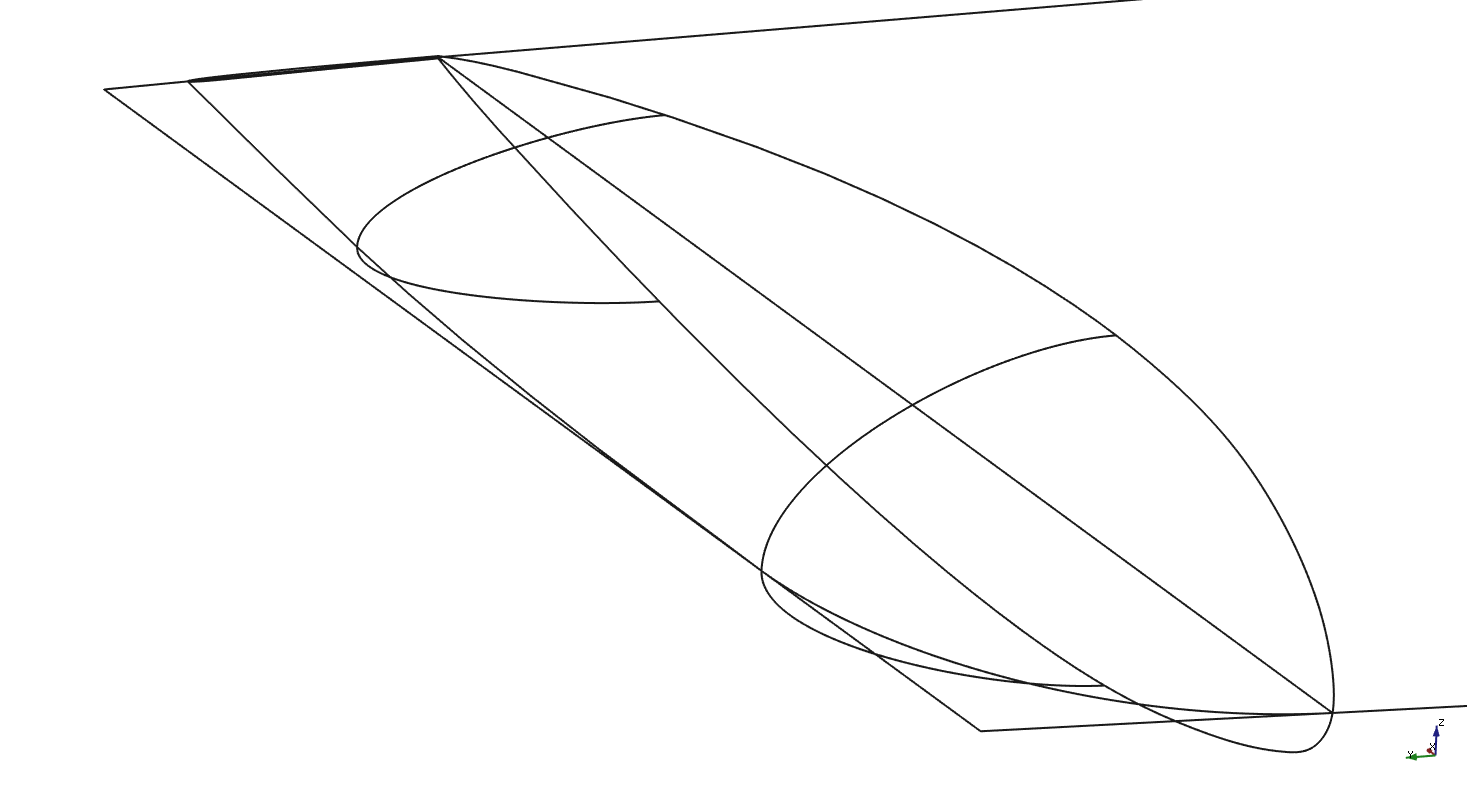
\includegraphics[scale=0.40]{Immagini/Capitolo3/WingTipWireframeMainSections}
\caption{Wing tip wireframe main supporting curves}
\label{fig:WingTip1}
\end{figure}
% 

\bigskip
\noindent
For the main supporting curves, namely those crossing the tip airfoil at the $25\%$, $75\%$ and $100\%$ in terms of its chord fraction, it is not necessary to calculate anything for the last entry of the \lstinline[language=Java]!createVerCrvsForTipClosure! method, since those points are the ones that have been used to determine the shape of the in-plane construction curve. When it comes to supporting curves between the main ones (which are necessary in order to make sure the tip patching process is successfully accomplished) some calculation is needed instead. First thing, spacings between these curves are established by means of three arrays (reported in listing \ref{lst:TipSubSupCurves}), one for each of the sections the wing tip has been split into by the previous step. These spacings are used directly to determine points on the in-plane construction curves by employing their parametric definition and their range. But once these points have been successfully obtained, what it is necessary to do, in order to use the same method described above in order to generate cross section curves, is determine their position in terms of wing tip chord fraction. This operation is quite simple to accomplish and involves just linear interpolation (provided by the \gls{JPAD} utility class \lstinline[language=Java]!MyMathUtils!) and some basic geometry consideration, and is reported in listing \ref{lst:TipSubSupCurves}. Once the necessary chord fractions have been obtained, the \lstinline[language=Java]!createVerCrvsForTipClosure! method can be used, and the resulting cross section curves are arranged in three different arrays, in order to be used later in the code. The \lstinline[language=Java]!double! arrays defining these sections follow a peculiar spacing, especially for the first one. These spacings have been chosen after performing several tests, while searching for the best results in terms of returned shapes. Figure \ref{fig:WingTip2} shows the final result for the wing tip wireframe.
%
\bigskip
\begin{lstlisting}[caption={Supporting curves between main wing tip cross sections}, captionpos=b, tabsize=2, label={lst:TipSubSupCurves}]
// Sub cross sections arrays		
double[] subVSecP1Vector = {0.10, 0.15, 0.40, 0.55, 0.60, 0.75, 0.90}; 
double[] subVSecP2Vector = {0.25, 0.50, 0.75};
double[] subVSecP3Vector = {0.25, 0.50, 0.75};

List<double[]> subVSecVector = new ArrayList<>();

subVSecVector.add(subVSecP1Vector);
subVSecVector.add(subVSecP2Vector);
subVSecVector.add(subVSecP3Vector);
				
List<CADGeomCurve3D[]> subVSecP1 = new ArrayList<>();
List<CADGeomCurve3D[]> subVSecP2 = new ArrayList<>();
List<CADGeomCurve3D[]> subVSecP3 = new ArrayList<>();	
List<List<CADGeomCurve3D[]>> subVSec = new ArrayList<List<CADGeomCurve3D[]>>();

// Iterate through the wing tip sections, in order 
// to generate additional  supporting curves
for(int i = 0; i < 3; i++) {
	int idx = i;
	subVSec.add(Arrays
		.stream(subVSecVector.get(i))
		.mapToObj(f -> {
			double[] crvRange = constrPlaneGuideCrvs.get(idx).getRange();
			double[] pntOnGuideCurve = constrPlaneGuideCrvs.get(idx)
							.value(f*(crvRange[1]-crvRange[0])+crvRange[0]);
			double interpCoord;
			double chordFraction;
			double x = pntOnGuideCurve[0];
			
			// Determine the corresponding chord fraction for the just  
			// calculated point lying on the construction curve
			if(!typeLS.equals(ComponentEnum.VERTICAL_TAIL)) {
				interpCoord = pntOnGuideCurve[1];
				double xLE = MyMathUtils.getInterpolatedValue1DLinear(
					new double[] {le2.y, aPnt.y}, 
					new double[] {le2.x, aPnt.x}, 
					interpCoord
			    		);
			    	double xTE = MyMathUtils.getInterpolatedValue1DLinear(
			    		new double[] {te2.y, bPnt.y}, 
			    		new double[] {te2.x, bPnt.x}, 
			    		interpCoord
			    		);
			    	chordFraction = (x - xLE)/(xTE - xLE);
			} else {
			    	interpCoord = pntOnGuideCurve[2];
			    	double xLE = MyMathUtils.getInterpolatedValue1DLinear(
			    		new double[] {le2.z, aPnt.z}, 
			    		new double[] {le2.x, aPnt.x}, 
			    		interpCoord
			    		);
			    	double xTE = MyMathUtils.getInterpolatedValue1DLinear(
			    		new double[] {te2.z, bPnt.z}, 
			    		new double[] {te2.x, bPnt.x}, 
			    		interpCoord
			    		);
			    	chordFraction = (x - xLE)/(xTE - xLE);
			}
			
			// Generate the supporting curve
			CADGeomCurve3D[] subVSecCrvs = createVerCrvsForTipClosure(
			    	liftingSurface, 
			    	airfoilTipCrvs,
			    	airfoilPreTipCrvs,
			    	new PVector[] {le1, le2},
			    	new PVector[] {te1, te2},
			    	chordFraction,
			    	pntOnGuideCurve
			    	);
			 return subVSecCrvs;
		})
		.collect(Collectors.toList())
		);
}

// Collect the additional supporting curves in three different arrays
subVSecP1.addAll(subVSec.get(0));
subVSecP2.addAll(subVSec.get(1));
subVSecP3.addAll(subVSec.get(2));
\end{lstlisting}
% 
\begin{figure}[H]
\centering
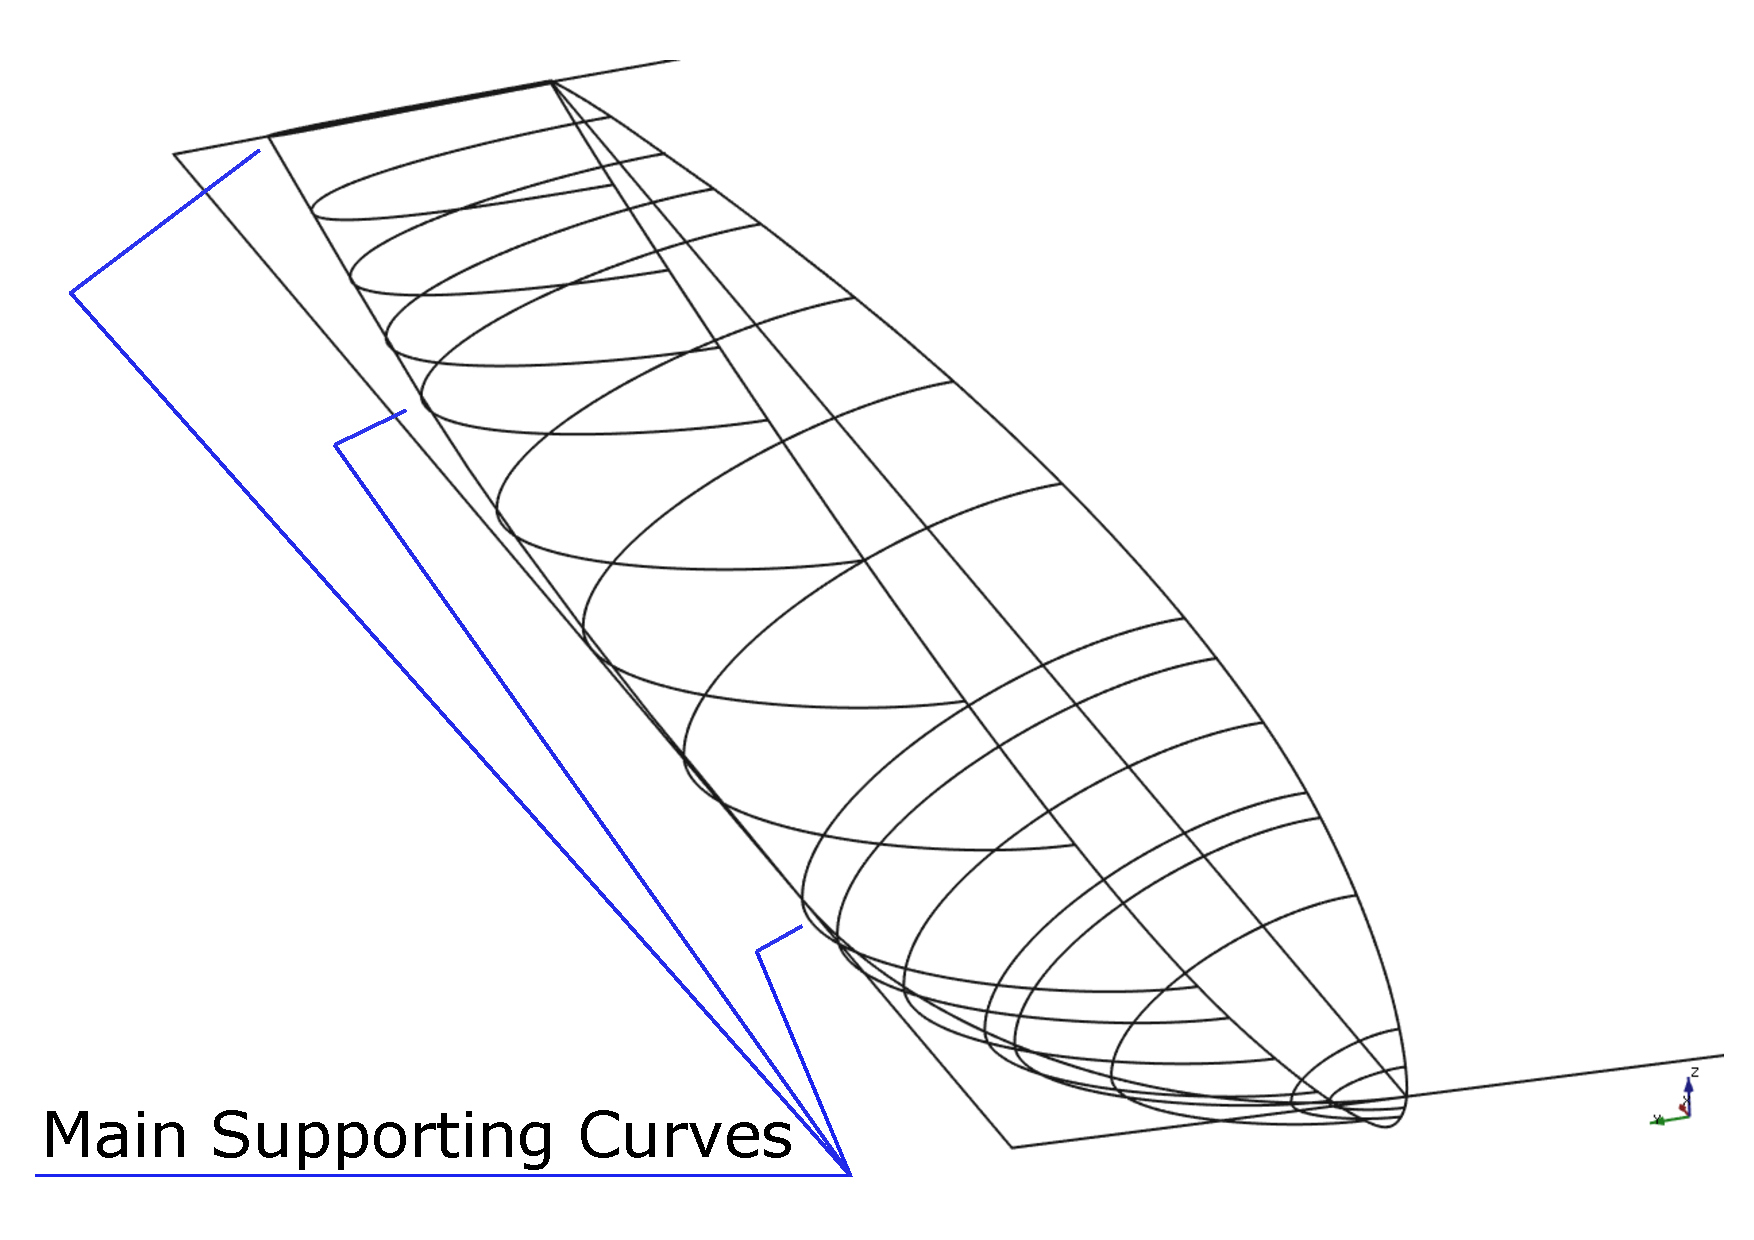
\includegraphics[scale=0.35]{Immagini/Capitolo3/wingtip_4}
\caption{Wing tip wireframe supporting curves}
\label{fig:WingTip2}
\end{figure}
% 

\bigskip
\noindent
Once the definitive wireframe has been built, it is finally possible to generate wing patches. The first ones to be created are those for the wing panels. The procedure is quite similar to the one used for the fuselage. The aforementioned list of lists, called \lstinline[language=Java]!cadCurveAirfoilList! and containing \lstinline[language=Java]!CADGeomCurve3D! entities representing airfoil curves, is used along with the \lstinline[language=Java]!makePatchThruSections! method in order to generate a loft for each panel. The piece of code below briefly explains the procedure, while figure \ref{fig:WingPanelPatches} depicts the results.
%
\bigskip
\begin{lstlisting}[caption={Spacings for supporting curves between main wing tip cross sections}, captionpos=b, tabsize=2, label={lst:TipSubSupCurves}]
List<OCCShape> patchWing = new ArrayList<>();
patchWing.addAll(cadCurveAirfoilList.stream()
		                   .map(OCCUtils::makePatchThruSections)
		                   .collect(Collectors.toList()));
\end{lstlisting}
% 
\begin{figure}[H]
\centering
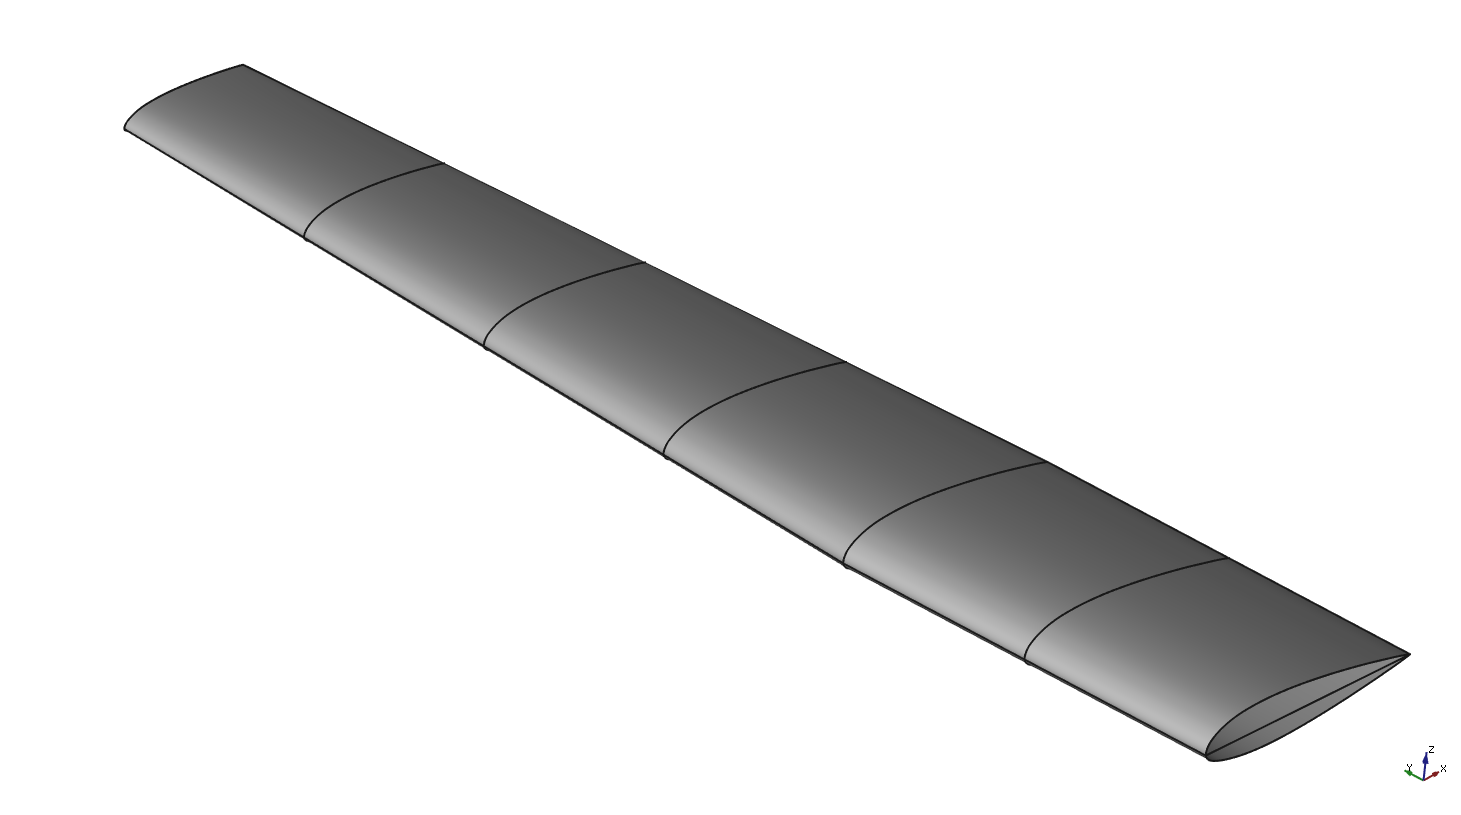
\includegraphics[scale=0.40]{Immagini/Capitolo3/WingPatches}
\caption{Main wing patches}
\label{fig:WingPanelPatches}
\end{figure}
% 

\bigskip
\noindent
Then it's the turn for the wing tip. The patching process can be divided in four stages, with the first one regarding the forward part of the wing tip. In order to obtain a smoother surface than the one that would be returned by simply using the \lstinline[language=Java]!makePatchThruSections! algorithm (the one involving curves and vertices), it has been decided to employ a different method and some different \gls{OCCT} classes. In particular, the choice has fallen on the \lstinline[language=Java]!BRepOffsetAPI_MakeFilling! class, which allows to generate filling surfaces by providing a set of curves bounding the face we want to generate, and a set of points defining some constraints the support face has to satisfy. In order to provide the bounding edges the algorithm requires, it has been necessary to split the first of the in-plane construction curves and the upper and lower curves defining the wing tip airfoil at the extremities of the second pair of supporting curves of the wing tip wireframe first section. This task has been accomplished by means of the \lstinline[language=Java]!OCCUtils! \lstinline[language=Java]!splitEdge! method. Then several points on the first of the supporting curves have been used as constraints for the final surface. In order to obtain the best result possible, two filling surfaces have actually been created, one for the upper side and one for the lower one. The following listing shows how the procedure has been coded, while figure \ref{fig:WingTipFilling} shows the final result.
%
\bigskip
\begin{lstlisting}[caption={Wing tip leading edge filling code, upper side}, captionpos=b, tabsize=2, label={lst:WingTipFilling}]
// Splitting the tip airfoil curves and the construction  
// curve #1 in order to fill the wing tip LE correctly
List<OCCEdge> airfoilUpperCrvs = new ArrayList<>();
airfoilUpperCrvs.addAll(OCCUtils.splitEdge(
		OCCUtils.theFactory.newCurve3D(airfoilTipCrvs.get(0)), 
		subVSecP1.get(1)[0].edge().vertices()[0].pnt()
		));
		
List<OCCEdge> constPlaneGuideCrvs1 = new ArrayList<>();
constPlaneGuideCrvs1.addAll(OCCUtils.splitEdge(
		constrPlaneGuideCrv1, 
		subVSecP1.get(1)[0].edge().vertices()[1].pnt()
		));

// Creating a filler surface at the wing tip leading edge, upper side.
// The procedure for the lower side pretty identical.			
double[] contrCrvUppRng = subVSecP1.get(0)[0].getRange();
double[] contrPntUpp1 = subVSecP1.get(0)[0].value(
		0.25*(contrCrvUppRng[1] - contrCrvUppRng[0]) + contrCrvUppRng[0]);
double[] contrPntUpp2 = subVSecP1.get(0)[0].value(
		0.50*(contrCrvUppRng[1] - contrCrvUppRng[0]) + contrCrvUppRng[0]);
double[] contrPntUpp3 = subVSecP1.get(0)[0].value(
		0.75*(contrCrvUppRng[1] - contrCrvUppRng[0]) + contrCrvUppRng[0]);

BRepOffsetAPI_MakeFilling fillerP1Upp = new BRepOffsetAPI_MakeFilling();

fillerP1Upp.Add(
		airfoilUpperCrvs.get(1).getShape(),
		GeomAbs_Shape.GeomAbs_C0);
fillerP1Upp.Add(
		((OCCEdge)((OCCGeomCurve3D)subVSecP1.get(1)[0]).edge()).getShape(),
		GeomAbs_Shape.GeomAbs_C0);
fillerP1Upp.Add(
		constPlaneGuideCrvs1.get(0).getShape(),
		GeomAbs_Shape.GeomAbs_C0);		

fillerP1Upp.Add(new gp_Pnt(contrPntUpp1[0], contrPntUpp1[1], contrPntUpp1[2]));
fillerP1Upp.Add(new gp_Pnt(contrPntUpp2[0], contrPntUpp2[1], contrPntUpp2[2]));
fillerP1Upp.Add(new gp_Pnt(contrPntUpp3[0], contrPntUpp3[1], contrPntUpp3[2]));

fillerP1Upp.Build();
\end{lstlisting}
% 
\bigskip
\begin{figure}[H]
\centering
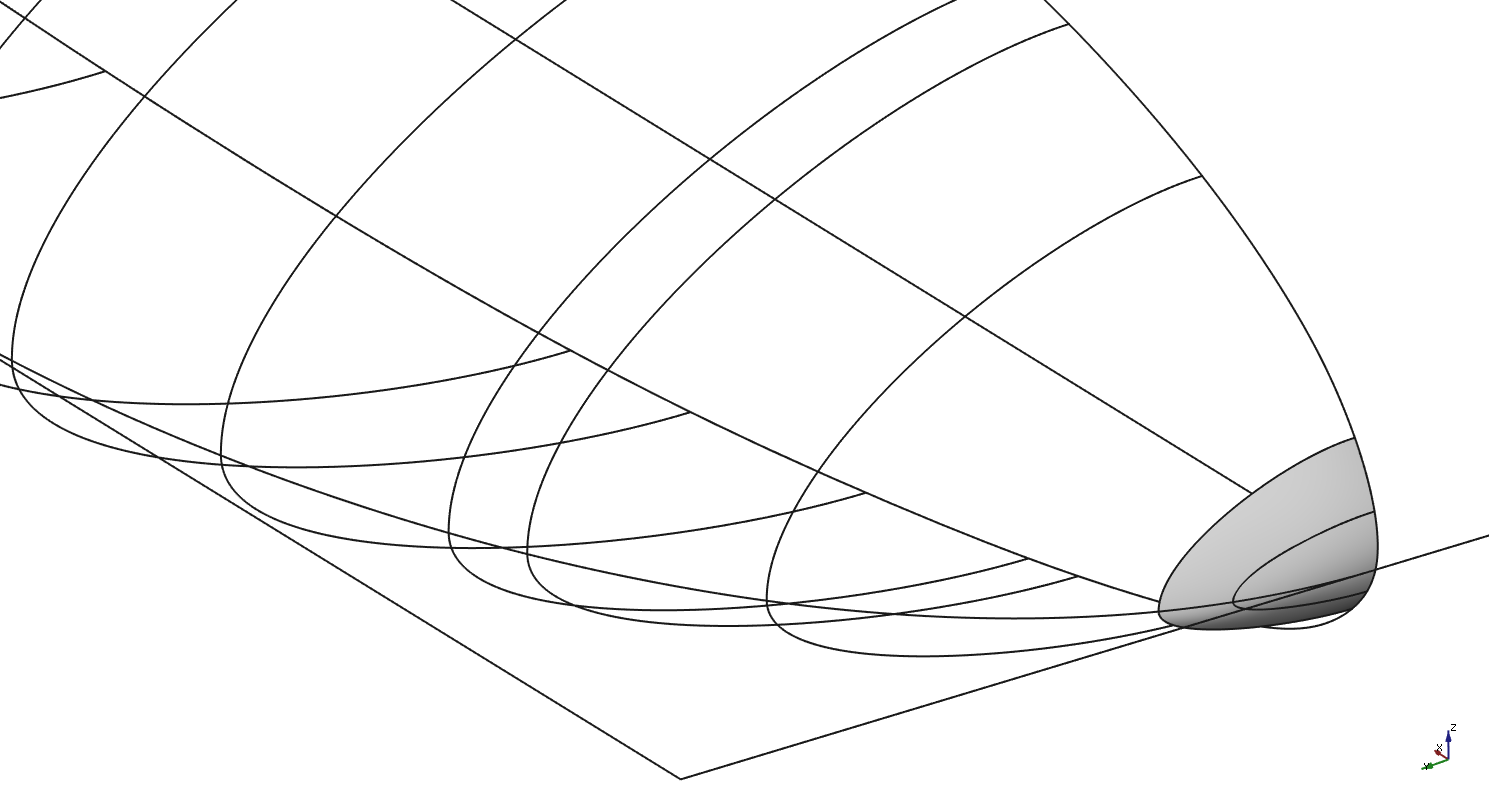
\includegraphics[scale=0.35]{Immagini/Capitolo3/WingTipLEFilling}
\caption{Wing tip leading edge filling surface}
\label{fig:WingTipFilling}
\end{figure}
%  

\bigskip
\noindent
The remaining sections of the wing tip are completed by means of the \lstinline[language=Java]!makePatchThruSections! algorithm. It has to be said that the second section (the one going from point C to point F, to be clear), has not been obtained in a single step (i.e., by patching through all the cross sections at the same time), but splitting the patching in two, in order to obtain the best result. This is the reason why, in the figures in which the final shell and solid shapes are depicted, the wing tip shell presents five patches rather than four, including the one obtained by the use of the filling algorithm. Figure \ref{fig:WingTipFinal} shows all the patches along with the supporting curves.
% 
\begin{figure}[H]
\centering
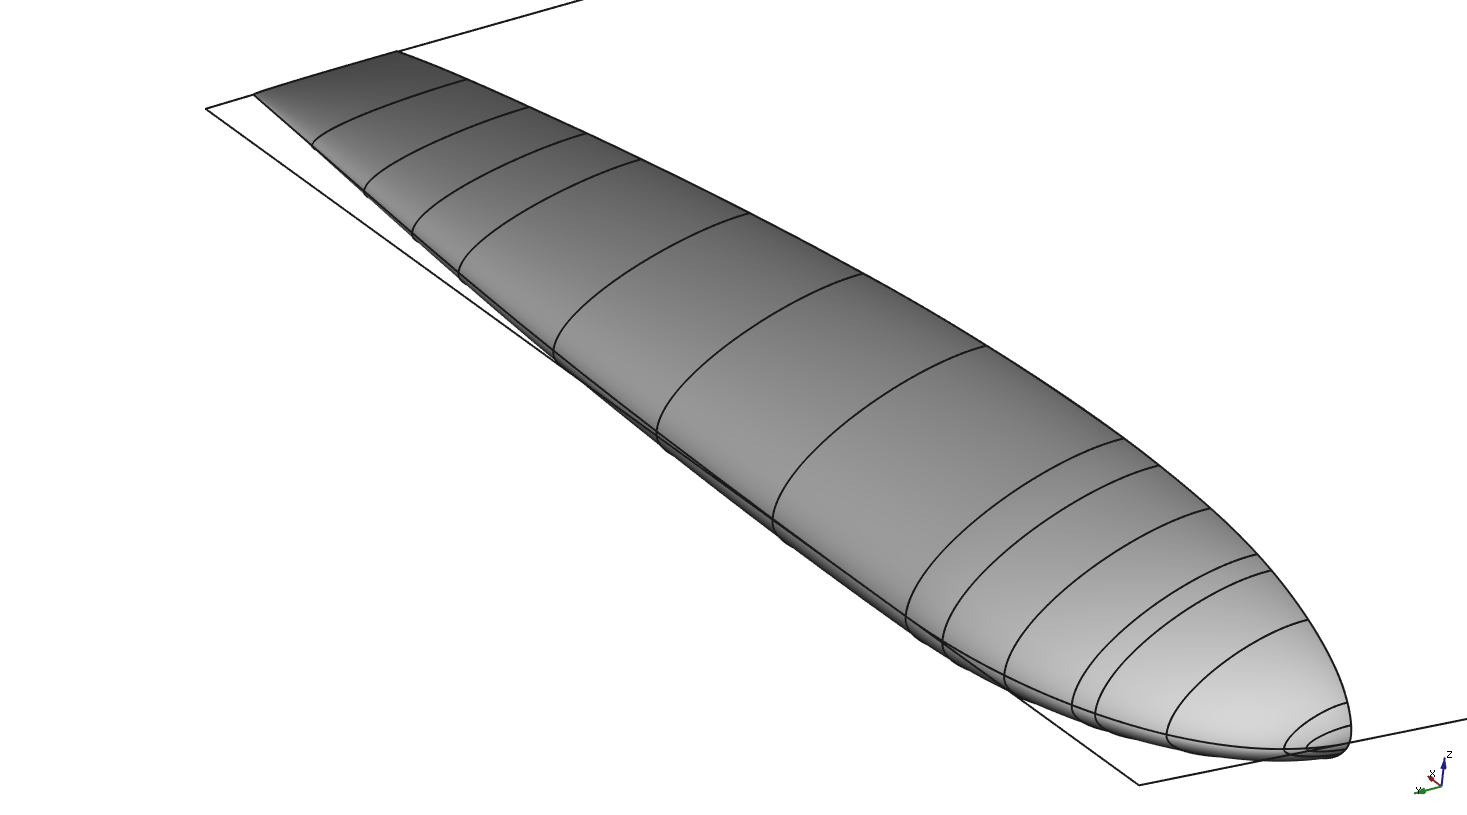
\includegraphics[scale=0.38]{Immagini/Capitolo3/WingTipPatches}
\caption{Wing tip patches and supporting curves}
\label{fig:WingTipFinal}
\end{figure}
%  

\bigskip
\noindent
Before sewing all the patches together in order to obtain one single shell, another step is needed. In fact, the aforementioned operation performed by the \lstinline[language=Java]!populateCoordinateList! method, consisting in opening the trailing edge of the airfoil whether necessary, has left some sort of hole on the back of the wing that must be filled. This operation has to be performed both for the panel patches and the wing tip, and the method that allows to do this is one of those listed in Chapter \ref{chap2}: the \lstinline[language=Java]!OCCUtils! static method \lstinline[language=Java]!makeFilledFace!. The \gls{OCCT} algorithm behind this method is provided by the same class used above, in order to fill the leading edge of the wing tip: \lstinline[language=Java]!BRepOffsetAPI_MakeFilling!. However, the way the algorithm is implemented in \lstinline[language=Java]!OCCUtils! allows just to determine the flat surface bounded by the curves the method is provided with. So, the method accepts an array of indefinite length of \lstinline[language=Java]!CADGeomCurve3D! entities, and returns the surface between the curves (which necessaryly must provide a closed wire). Figure \ref{fig:WingTipTE} shows the filling surface for the trailing edge of the wing tip.
% 
\begin{figure}[H]
\centering
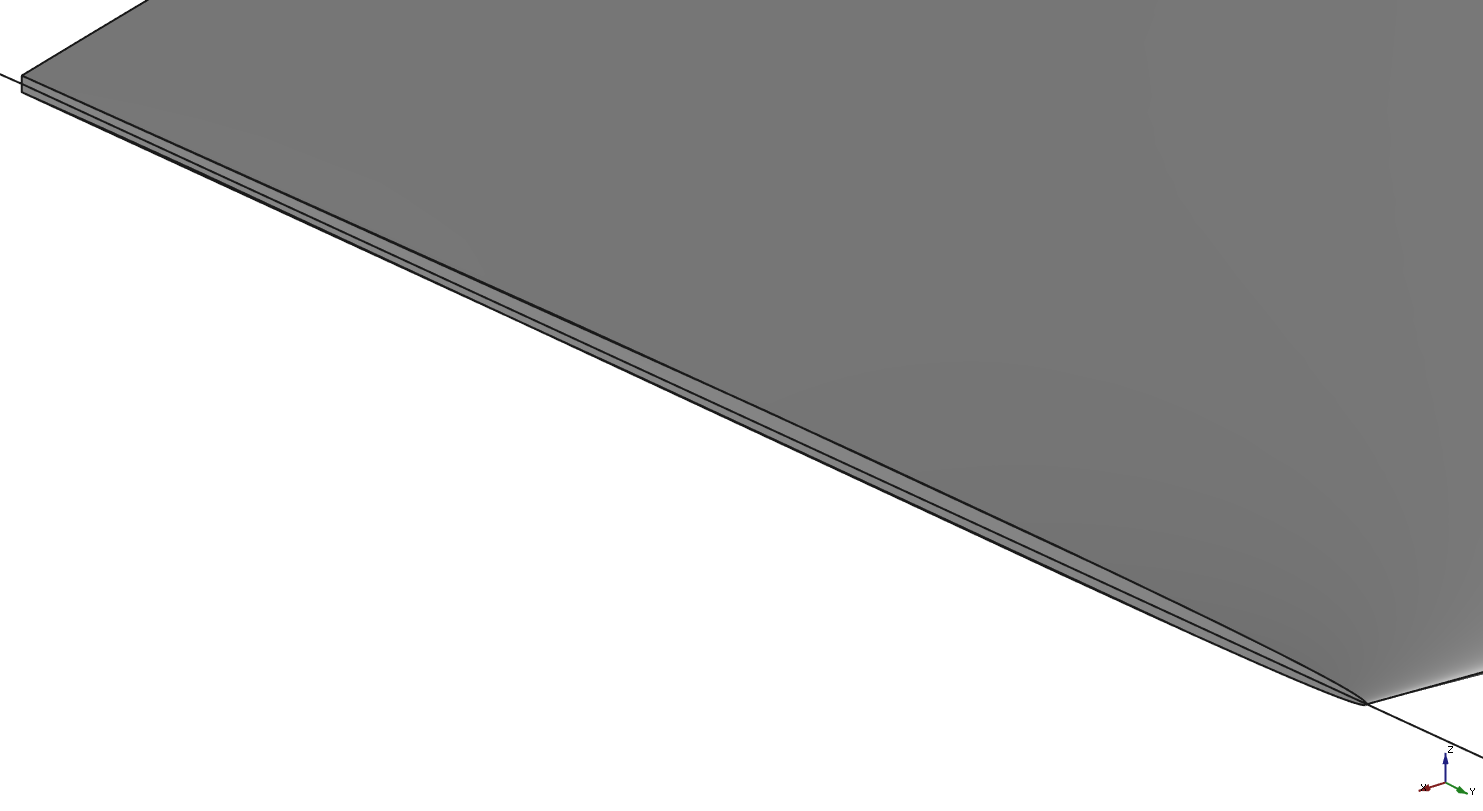
\includegraphics[scale=0.30]{Immagini/Capitolo3/WingTipTEFilledFace}
\caption{Wing tip trailing edge filling surface}
\label{fig:WingTipTE}
\end{figure}
%  

\bigskip
\noindent
The next steps consist in sewing all the patches and the faces created till now. First, wing panel patches are sewed, along with the trailing edge filling surfaces mentioned above. Then it is necessary to sew together the wing tip patches. This operation is much more delicate than the preceding one, since in this case the curves that define the borders of the patches we want to sew do not exactly coincide. This is due to the use of the edge splitting algorithm, which sligthly modify the returning curves respect to the original one. In order to overcome this problem, the default tolerance of the sewing algorithm has been changed, and set to the value which is provided as input to the \lstinline[language=Java]!getLiftingSurfaceCAD! method. For the same reasons, the default tolerance for the sewing algorithm needs to be set to a different (higher) value when sewing the wing tip shell with the one obtained by sewing the panel lofts. In this case, in particular, the difference between the two shells is much more evident, due to the fact that they have been obtained by patching through sections following different (orthogonal) directions.

\bigskip
\noindent
The following operations are pretty much the same conducted for the fuselage solid construction. The main difference consists in the fact that mirroring operations are not necessary in case the lifting surface is a vertical tail. In fact, in this case, the only necessary operation consists in closing the side of the shell which is still open (i.e., the side opposite to the one where the wing tip has been built). The following piece of code (listing \ref{lst:VerticalTailClosing}) shows how this operation has been implemented in the \lstinline[language=Java]!getLiftingSurfaceCAD! algorithm. Again, the method this operation makes use of is the \lstinline[language=Java]!OCCUtils! static function \lstinline[language=Java]!makeFilledFace!.
%
\bigskip
\begin{lstlisting}[caption={Vertical tail filling operations}, captionpos=b, tabsize=2, label={lst:VerticalTailClosing}]
// Check whether the lifting surface is a vertical tail
if(typeLS.equals(ComponentEnum.VERTICAL_TAIL)) {
		CADShape faceRoot = OCCUtils.makeFilledFace(
		
		 		// Get the first of the airfoil curves
				cadCurveAirfoilList.get(0).get(0),  
				
				// Create a segment representing the trailing
				// edge of the first of the airfoil curves
				OCCUtils.theFactory.newCurve3D( 
						cadCurveAirfoilList.get(0).get(0).edge().vertices()[0].pnt(), 
						cadCurveAirfoilList.get(0).get(0).edge().vertices()[1].pnt()
						) 
				);
				
		// Add this shape to the ones to be sewed	
		sewMakerWing.Add(((OCCShape) faceRoot).getShape()); 
}		
\end{lstlisting}

\bigskip
\noindent
In case the lifting surface is not a vertical tail, mirroring, sewing, and solid generating operations are performed by means of the same methods and classes listed above, for the fuselage \gls{CAD} problem. In this case too, the method allows to export just the desired shapes: by setting the previously mentioned \lstinline[language=Java]!boolean! arguments, the user can decide which types of shapes he wants to extract. Figure \ref{fig:WingSolid} shows the final result in terms of solid shapes. In particular, the depicted wing is the one of the ATR-72. The following paragraphs will also provide more examples of lifting surfaces produced by means of the same algorithm.
% 
\begin{figure}[H]
\centering
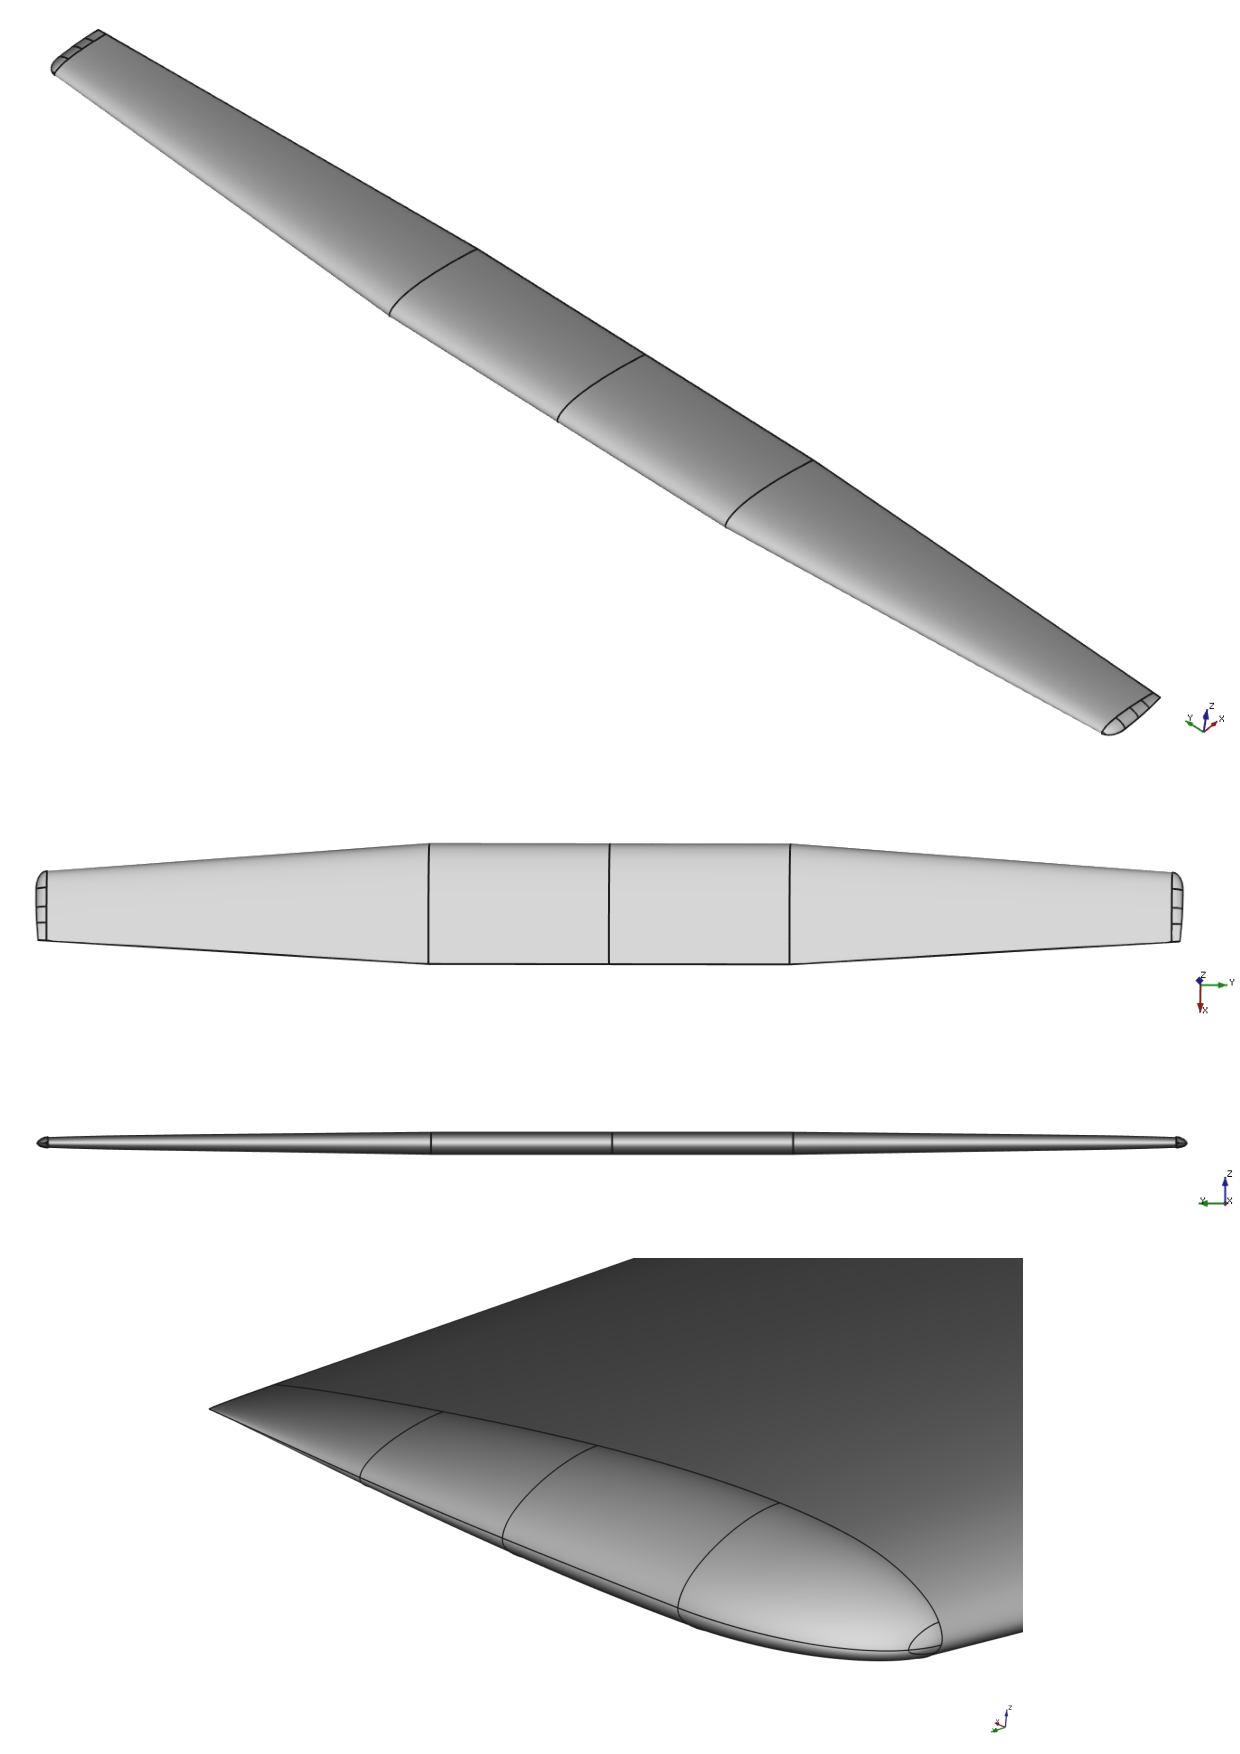
\includegraphics[scale=0.68]{Immagini/Capitolo3/wing_2}
\caption{ATR-72 solid wing, with a close-up on the wing tip}
\label{fig:WingSolid}
\end{figure}
%  

\section{\texttt{AircraftUtils} additional methods}
\label{sec3.5}
The methods analyzed in the previous paragraphs provide just the necessary tools to build \gls{CAD} shapes out of data stored in \gls{JPAD} aircraft classes. In order to actually be able to import aircraft data from files and write generated \gls{CAD} shapes to specific file formats, \lstinline[language=Java]!AircraftUtils! needs to be filled with additional methods. This paragraph gives an overview on the extra functions (and sub-classes) contained in \lstinline[language=Java]!AircraftUtils!, providing basic information on how they work and the classes they make use of.

\subsection{\texttt{importAircraft}}
\label{sec3.5.1}

The \lstinline[language=Java]!importAircraft! method is the tool that has been used in \lstinline[language=Java]!JPADCADSandbox! tests in order to actually import aircraft data from XML files and populate instances of the \gls{JPAD} \lstinline[language=Java]!aircraft! class. The operations performed by this method rely on an important Java library: \lstinline[language=Java]!args4j! \cite{args4j}. In short, \lstinline[language=Java]!args4j! library provides classes that allow to parse command line options. In this way, the paths to the directories and the files containing the necessary information to build new \lstinline[language=Java]!aircraft! instances can be easily managed and passed to the \gls{JPAD} utilities that provide support to XML file reading operations. In particular, the \lstinline[language=Java]!importAircraft! method accepts just one parameter, of the Java \lstinline[language=Java]!String[]! type, that contains the list of all the necessary directories. This list must be written according to the same notation used for the definition of the options of a supporting class (which in the present case has been called \lstinline[language=Java]!ArgumentsJPADCADSandbox!) that, along with the \lstinline[language=Java]!args4j! \lstinline[language=Java]!CmdLineParser! class, actually performs the parsing of the command line. Once the input array has been parsed, it is finally possible to populate the \lstinline[language=Java]!aircraft! object, by means of the \lstinline[language=Java]!JPADXmlReader! class. An example of usage of this method is given in paragraph \ref{sec3.6}.

\subsection{\texttt{enum} classes}
\label{sec3.5.2}

The \lstinline[language=Java]!AircraftUtils! class contains two Java \lstinline[language=Java]!enum! classes, which have yet been mentioned in the previous paragraphs. What follows focuses on their definitions and their usage.

\subsubsection{\texttt{FileExtension}}

This \lstinline[language=Java]!enum! class is used to enumerate all the possible file formats, supported by the \gls{OCCT} library, that can be used to save \gls{CAD} entities. In particular, this class is used by another \lstinline[language=Java]!AircraftUtils! method, which is explained just below, in order to select the right operations to perform for the purpose of writing \gls{CAD} shapes to a specific file format. Listing \ref{lst:FileExtension} reports the structure of this \lstinline[language=Java]!enum! class.
%
\bigskip
\begin{lstlisting}[caption={\lstinline!FileExtension! class}, captionpos=b, tabsize=2, label={lst:FileExtension}]
public enum FileExtension {
		BREP,
		STEP,
		IGES,
		STL;
}
\end{lstlisting}

\subsubsection{\texttt{XSpacingType}}

The \lstinline[language=Java]!XSpacingType! class is used to enumerate the spacings that it is possible to employ once being provided an interval and the number of points that must be contained in the interval. In addition to the definitions of the elements of the class, it also contains an abstract method, named \lstinline[language=Java]!calculateSpacing!, that it is implemented by each one of the enumerators (listing \ref{lst:XSpacingType}). This \lstinline[language=Java]!enum! class is used by the \lstinline[language=Java]!getFuselageCAD! method in order to define the spacing for the cross sections of the nose and the tail trunks.
%
\bigskip
\begin{lstlisting}[caption={\lstinline!XSpacingType! class}, captionpos=b, tabsize=2, label={lst:XSpacingType}]
public enum XSpacingType {
		UNIFORM {
				@Override
				public Double[] calculateSpacing(double x1, double x2, int n) {
						Double[] xSpacing = MyArrayUtils.linspaceDouble(x1, x2, n);
						return xSpacing;
				}
		},
		COSINUS {
				@Override
				public Double[] calculateSpacing(double x1, double x2, int n) {
						Double[] xSpacing = MyArrayUtils.cosineSpaceDouble(x1, x2, n);
						return xSpacing;
				}
		},
		HALFCOSINUS1 { // finer spacing close to x1
				@Override
				public Double[] calculateSpacing(double x1, double x2, int n) {
						Double[] xSpacing = MyArrayUtils.halfCosine1SpaceDouble(x1, x2, n);
						return xSpacing;
				}
		}, 
		HALFCOSINUS2 { // finer spacing close to x2
				@Override
				public Double[] calculateSpacing(double x1, double x2, int n) {
						Double[] xSpacing = MyArrayUtils.halfCosine2SpaceDouble(x1, x2, n);
						return xSpacing;
				}
		}; 
		
		public abstract Double[] calculateSpacing(double x1, double x2, int n);
}
\end{lstlisting}

\subsection{CAD methods overload}
\label{sec3.5.3}

One of the most important characteristics of a language such as Java is the possibility to perform methods overloading. Method overloading is a feature that allows a class to have more than one method having the same name, if their argument lists are different. For this reason, it is possible to define various \lstinline[language=Java]!getLiftingSurfaceCAD! and \lstinline[language=Java]!getFuselageCAD!, differing from each other for the arguments they support. The following listing reports all the different versions for the aforementioned methods currently contained in \lstinline[language=Java]!AircraftUtils!.
\bigskip
\begin{lstlisting}[caption={CAD generating methods overloading in \lstinline!AircraftUtils!}, captionpos=b, tabsize=2, label={lst:MethodOverloading}]
public static List<OCCShape> getFuselageCAD(Fuselage fuselage,
			double noseCapSectionFactor1, double noseCapSectionFactor2, 
			int numberNoseCapSections, 
			int numberNosePatch2Sections, XSpacingType spacingTypePatch2, 
			int numberTailPatchSections, XSpacingType spacingTypeTailPatch, 
			double tailCapSectionFactor1, double tailCapSectionFactor2, 
			int numberTailCapSections,
			boolean exportLofts, boolean exportSolids, boolean exportSupportShapes) {
			
			...
}

public static List<OCCShape> getFuselageCAD(Fuselage fuselage, 
			boolean exportSupportShapes) {

		return getFuselageCAD(fuselage, 
				0.15, 1.0, 3, 
				7, XSpacingType.COSINUS, 
				7, XSpacingType.COSINUS, 
				1.0, 0.15, 3, 
				true, true, exportSupportShapes);
}

public static List<OCCShape> getFuselageCAD(Fuselage fuselage, 
			boolean exportLofts, boolean exportSolids, boolean exportSupportShapes) {
			
		return getFuselageCAD(fuselage, 
				0.15, 1.0, 3, 
				7, XSpacingType.COSINUS, 
				7, XSpacingType.COSINUS, 
				1.0, 0.15, 3, 
				exportLofts, exportSolids, exportSupportShapes);
}

public static List<OCCShape> getFuselageCAD(Fuselage fuselage, 
			int numberNosePatch2Sections, int numberTailPatchSections, 
			boolean exportLofts, boolean exportSolids, boolean exportSupportShapes) {
		
		return getFuselageCAD(fuselage,
				0.15, 1.0, 3,
				numberNosePatch2Sections, XSpacingType.COSINUS,
				numberTailPatchSections, XSpacingType.COSINUS,
				1.0, 0.15, 3, 
				exportLofts, exportSolids, exportSupportShapes);
}

public static List<OCCShape> getLiftingSurfaceCAD(LiftingSurface liftingSurface, 
			ComponentEnum typeLS,
			double tipTolerance,
			boolean exportLofts,
			boolean exportSolids,
			boolean exportSupportShapes) {
			
			...
}

public static List<OCCShape> getLiftingSurfaceCAD(LiftingSurface liftingSurface, 
			ComponentEnum typeLS,
			boolean exportSupportShapes) {
		
		return getLiftingSurfaceCAD(liftingSurface,
				typeLS,
				1e-3,
				true,
				true,
				exportSupportShapes);
}
\end{lstlisting}

\bigskip
\noindent
\lstinline[language=Java]!AircraftUtils! also contains a method, called \lstinline[language=Java]!getAircraftShapes!, that allows to perform more than just one 
\gls{CAD} generating operation at a time, meaning that fuselage and lifting surface shapes can be generated at the same time by using one single method. In particular, the method accepts an object representing the aircraft, and a list containing values of the \gls{JPAD} \lstinline[language=Java]!ComponentEnum! class, specifying which type of shapes (i.e., fuselage, wing, tail, canard) must be produced. Then the method returns a list containing all the generated \lstinline[language=Java]!OCCShape! objects (listing \ref{lst:getAircraftShapes}).
\bigskip
\begin{lstlisting}[caption={\lstinline!getAircraftShapes! method}, captionpos=b, tabsize=2, label={lst:getAircraftShapes}]
public static List<OCCShape> getAircraftShapes(
			Aircraft theAircraft,
			List<ComponentEnum> components
			) {		
		List<OCCShape> allShapes = new ArrayList<>();
		
		if(theAircraft.getFuselage() != null && 
		   components.contains(ComponentEnum.FUSELAGE)) {
			allShapes.addAll(getFuselageCAD(theAircraft.getFuselage(), true));
		}		
		if(theAircraft.getWing() != null && 
		   components.contains(ComponentEnum.WING)) {
			allShapes.addAll(getLiftingSurfaceCAD(theAircraft.getWing(), 
				ComponentEnum.WING, 1e-3, true, true, true));
		}		
		if(theAircraft.getHTail() != null && 
		   components.contains(ComponentEnum.HORIZONTAL_TAIL)) {		
			allShapes.addAll(getLiftingSurfaceCAD(theAircraft.getHTail(), 
				ComponentEnum.HORIZONTAL_TAIL, 1e-3, true, true, true));
		}		
		if(theAircraft.getVTail() != null && 
		   components.contains(ComponentEnum.VERTICAL_TAIL)) {		
			allShapes.addAll(getLiftingSurfaceCAD(theAircraft.getVTail(), 
				ComponentEnum.VERTICAL_TAIL, 1e-3, true, true, true));
		}			
		if(theAircraft.getCanard() != null && 
		   components.contains(ComponentEnum.CANARD)) {		
			allShapes.addAll(getLiftingSurfaceCAD(theAircraft.getCanard(), 
				ComponentEnum.CANARD, 1e-3, true, true, true));
		}			
		return allShapes;
	}
\end{lstlisting}

\subsection{\texttt{getAircraftSolidFile}}
\label{sec3.5.4}

The \lstinline[language=Java]!getAircraftSolidFile! method allows to write solid shapes to file. It requires a Java \gls{List} containing generic \lstinline[language=Java]!OCCShape! entities, a \lstinline[language=Java]!String! standing for the name of the file we want to write, and an element of the \lstinline[language=Java]!FileExtension! class, which specifies the format of the file to be written. The first operation the method performs consists in filtering the input shapes, collecting all the solids found in one single list. This operation is made through the use of another \lstinline[language=Java]!AircraftUtils! static method, called \lstinline[language=Java]!getAircraftSolid!. Once all the solids have been obtained, the algorithm automatically chooses, by use of a switch statement, the right operations to perform in order to obtain a file in the format specified by the user. Currently the method supports writing in the following extensions:
%
\begin{itemize}
\item \gls{BRep},
\item STEP,
\item IGES,
\item STL.
\end{itemize}
%
All the writing operations rely on particular \gls{OCCT} classes, each one dedicated to a specific file format.

\section{Example}
\label{sec3.6}

The following example gives an idea of how the previously described methods can be used to automatically generate the \gls{CAD} model of an aircraft. For this purpose, a simple testing class has been created in \lstinline[language=Java]!JPADCADSandbox!. This class contains a main method that receives as input a \lstinline[language=Java]!String[]!, containing the paths to the directories that contain the XML files from which we want to read the aircraft data. The first operation consists in importing this data and fill in the \emph{fields} of a new \lstinline[language=Java]!Aircraft! object. This operation is conducted by using the \lstinline[language=Java]!importAircraft! method, by providing it with the aforementioned \lstinline[language=Java]!String! array. The next step consists in generating new instances of the \lstinline[language=Java]!Fuselage! and \lstinline[language=Java]!LiftingSurface! classes by making use of the methods of the \lstinline[language=Java]!Aircraft! class. Once they have been obtained, \gls{CAD} generating methods can be launched, by selecting one of the methods seen in section \ref{sec3.5.3}. In order to obtain the solid of the aircraft and write it to file (for the purpose of using it later, for example, in a \gls{CAD} or a \gls{CFD} software), the \lstinline[language=Java]!getAircraftSolidFile! method described above can be used, by providing it with the shapes we want to write, and the name and the format of the file (listing \ref{lst:Example01}).
%
\bigskip
\begin{lstlisting}[caption={Usage of \lstinline!AircraftUtils! methods}, captionpos=b, tabsize=2, label={lst:Example01}]
public class Test {

	public static void main(String[] args) {

		System.out.println("JPADCADSandbox Test");
		
		// Import aircraft data from XML files
		Aircraft aircraft = AircraftUtils.importAircraft(args);	
		
		// Generate instances of the JPAD 
		// classes describing aircraft components
		Fuselage fuselage = aircraft.getFuselage();	
		LiftingSurface wing = aircraft.getWing();		
		LiftingSurface hTail = aircraft.getHTail();
		LiftingSurface vTail = aircraft.getVTail();
		
		// Generate CAD shapes for all the aircraft components
		// and add them to a single List, in order to be exported
		List<OCCShape> allShapes = new ArrayList<>();
		
		List<OCCShape> fuselageShapes = AircraftUtils.getFuselageCAD(
				fuselage, 7, 7, true, true, true);
				
		List<OCCShape> wingShapes = AircraftUtils.getLiftingSurfaceCAD(
				wing, ComponentEnum.WING, 1e-3, true, true, true);
				
		List<OCCShape> hTailShapes = AircraftUtils.getLiftingSurfaceCAD(
				hTail, ComponentEnum.HORIZONTAL_TAIL, 1e-3, true, true, true);
				
		List<OCCShape> vTailShapes = AircraftUtils.getLiftingSurfaceCAD(
				vTail, ComponentEnum.VERTICAL_TAIL, 1e-3, true, true, true);	
				
		allShapes.addAll(fuselageShapes);
		allShapes.addAll(wingShapes);
		allShapes.addAll(hTailShapes);
		allShapes.addAll(vTailShapes);
		
		// Filter the shape list in order to collect the solid
		// ones only, and write them to STEP file format
		AircraftUtils.getAircraftSolidFile(allShapes, "aircraft", FileExtension.STEP);
	}
}
\end{lstlisting}

\bigskip
\noindent
Instead of generating \gls{CAD} shapes for each component at a time, one could have chosen to use the \lstinline[language=Java]!getAircraftShapes! method and provide it with the list of desired aircraft components (listing \ref{lst:Example02}). The results would have been exactly the same.
%
\bigskip
\begin{lstlisting}[caption={Usage of \lstinline!getAircraftShapes! method}, captionpos=b, tabsize=2, label={lst:Example02}]
		List<ComponentEnum> componentList = new ArrayList<>();
		componentList.add(ComponentEnum.FUSELAGE);
		componentList.add(ComponentEnum.WING);
		componentList.add(ComponentEnum.HORIZONTAL_TAIL);
		componentList.add(ComponentEnum.VERTICAL_TAIL);
		
		allShapes.addAll(AircraftUtils.getAircraftShapes(
				aircraft, componentList));
\end{lstlisting}

\bigskip
\noindent
Figure \ref{fig:Example01} shows the \gls{CAD} solid models of four different aircrafts obtained by using the same test along with the same methods listed above. It has to be noted how the same algorithm, \lstinline[language=Java]!getLiftingSurfaceCAD!, succeeds at building \gls{CAD} shapes for very different lifting surfaces, revealing to be quite versatile.
% 
\begin{figure}[H]
\centering
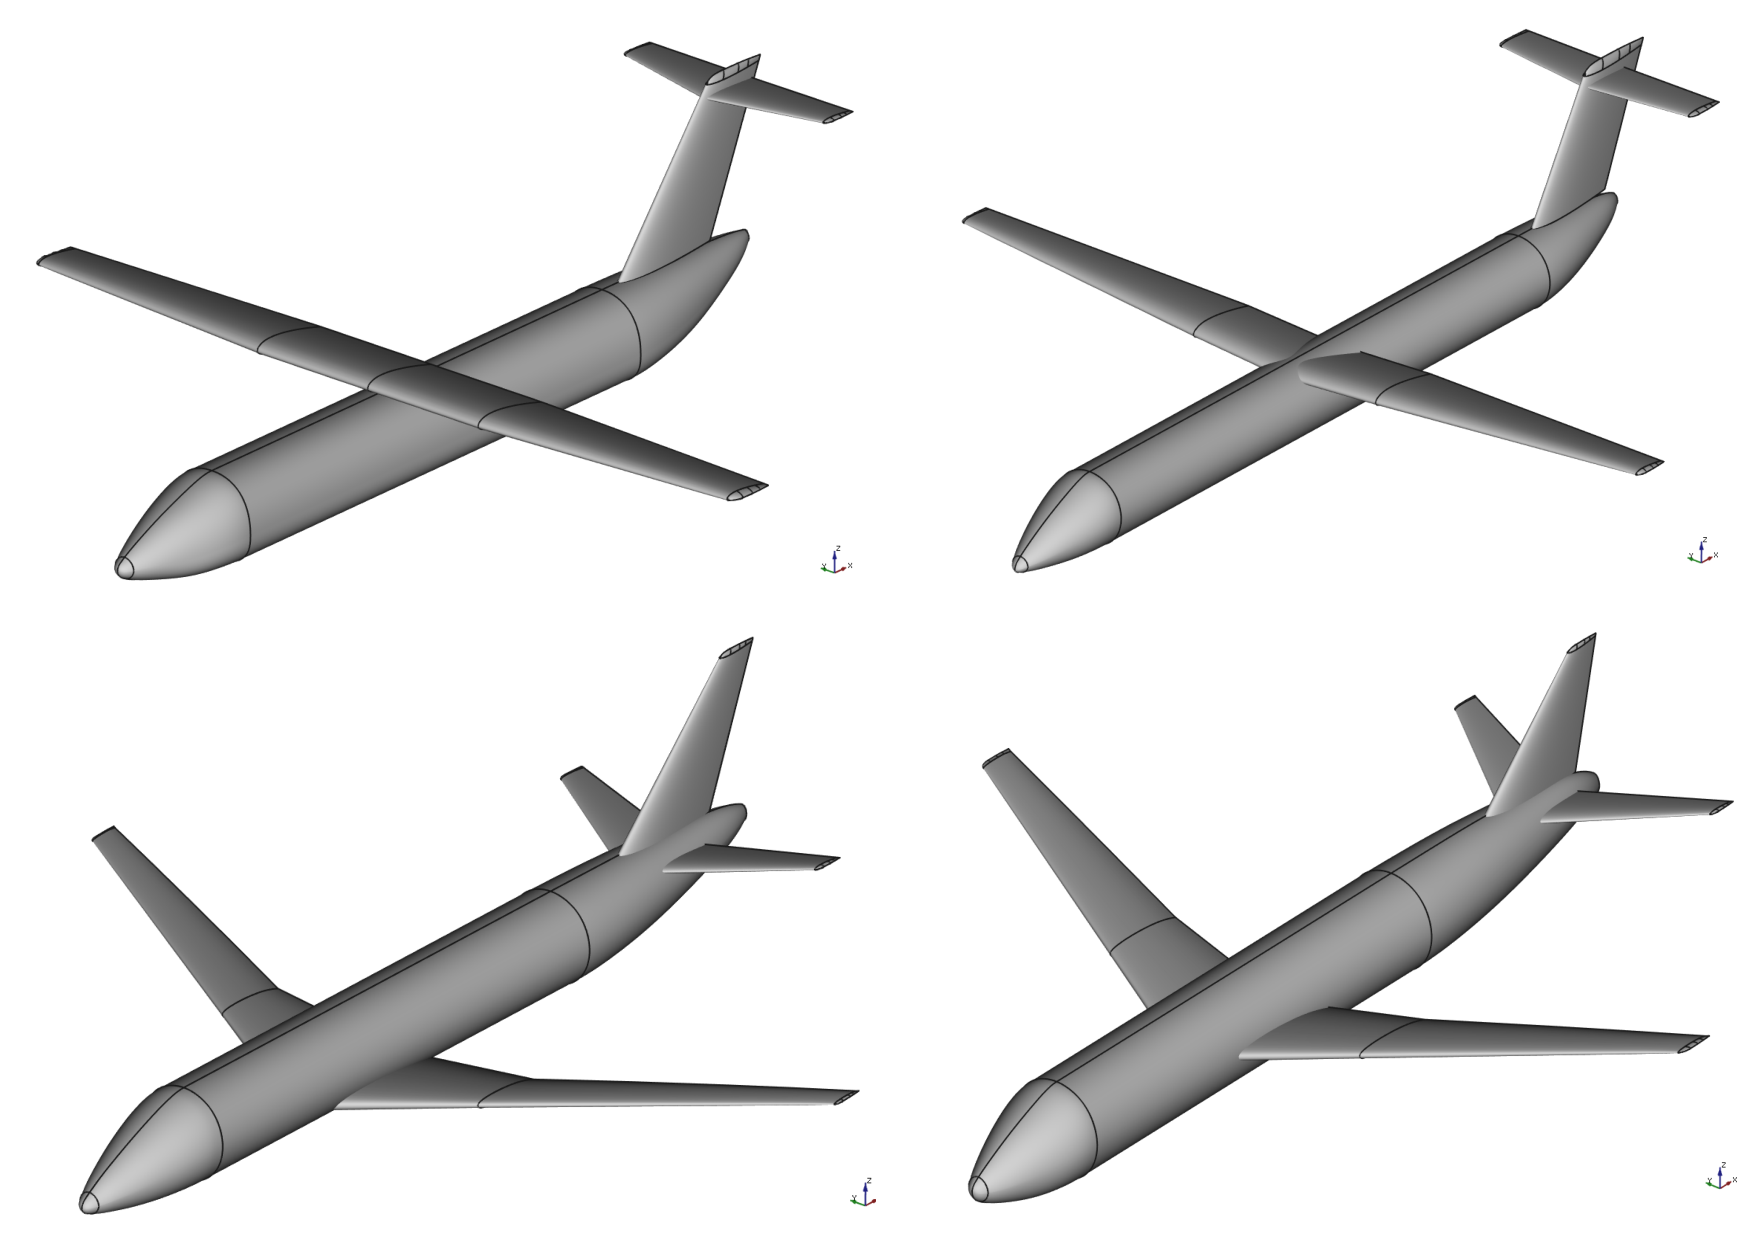
\includegraphics[scale=0.45]{Immagini/Capitolo3/Aircrafts/aircrafts_1}
\caption{Comparison between different aircraft CAD models obtained by using the same test class}
\label{fig:Example01}
\end{figure}
%  

\chapter{Automatic workflows for aerodynamic simulations}
\label{chap4}

\section{Introduction}
\label{sec4.1}

Since the very beginning, the main purpose behind the development of a library devoted to the automatic generation of 3D \gls{CAD} models of aircrafts has been the possibility of using the same models for aerodynamic analyses, carried out by the use of a \gls{CFD} software. For this reason, the models produced by \gls{JPAD} come equipped with solutions (such as the modeling of the wing tip, or the automatic gap enhancement of the aifoils trailing edge in case of necessity) that make them ready to be imported and used into a suite for aerodynamics investigations. Moreover, since the models are generated without the necessity of human intervention during the process, and considering that the classes of \gls{JPAD} offer the possibility to make changes to the geometric characteristics of aircraft components once imported from data file, what comes to mind is the possibility to integrate the \lstinline[language=Java]!JPADCAD! module, along with the \lstinline[language=Java]!AircraftUtils! functionalities, in a comprehensive development cycle involving \gls{CFD} analyses. By use of the aforementioned functions and classes, in fact, it becomes possible to automatically produce several geometries of the same aircraft, differing in some characteristics (e.g., the wing aspect ratio, or the dihedral angle). These models should be then imported, one at a time and in an automatic way, into a software for Computational Fluid Dynamics, in order to perform on them all the necessary analyses and produce the requested results. What becomes necessary at this point is some sort of \emph{bridge}, connecting \gls{JPAD} and all its modules to some existing \gls{CFD} software. This software, however, based on what has been said above, must fulfill the following requirements:
%
\begin{itemize}
\item must provide support for recording and playing macros,
\item must give the possibility to run macros in batch mode.
\end{itemize}   
%
These macros are going to collect all the operations that will be performed by the \gls{CFD} software, from importing the \gls{CAD} models to collecting results. In this way, one can think to launch a complete workflow from a simple test class (i.e., a class containing just a main method) located in \gls{JPAD}, which manages all the operations, from establishing the type of the analysis to actually running the software and the macro. 

\bigskip
\noindent
Therefore a choice needs to be made about the \gls{CFD} software. CD-adapco STAR-CCM+ meets the characteristics listed above. In addition, STAR-CCM+ macros are written in Java, with this representing a great advantage, since \gls{JPAD} is written in Java too. In fact, in order for our Java macros to run properly and perform operations as we want, it is necessary to provide them support by means of dedicated classes and utilities. These classes not only are used by the macros, but can also be employed by the test class in \gls{JPAD} in order to define the characteristics of the simulations, as it will be clearer in the following paragraphs. 

\section{STAR-CCM+ overview}
\label{sec4.2}

STAR-CCM+ is not just a tool for \gls{CFD} analyses. More in general, it is a \gls{CAE} solution for solving multidisciplinary problems in both fluid and solid continuum mechanics, within a single integrated interface. The STAR-CCM+ environment offers all the tools required in order to execute engineering analyses. These tools allows the following operations:
%
\begin{itemize}
\item import and creation of geometries,
\item mesh generation,
\item solution of the governing equations,
\item analysis of the results,
\item automation of the simulation workflows for design exploration studies,
\item connection to other \gls{CAE} software for co-simulation analysis.
\end{itemize}
%
For what concerns geometries, STAR-CCM+ can read geometric data saved in neutral formats (such as IGES and STEP) or triangulated ones (such as STL). Besides, it also offers a built-in capability for modifying and creating \gls{CAD} geometries directly. Its 3D \gls{CAD} tool is a parametric feature-based modeler that is built upon the Parasolid kernel. Among its extensive suite of \gls{CAD} functions it includes important operations, such as Boolean actions, automatic removal of small bodies or surfaces irrelevant to simulation, and flow domain extraction. Regarding mesh operations, STAR-CCM+ provides a complete set of capabilities for both surface and volume meshing operations. Its mesh framework provides a flexible environment and, most importantly, repeatable processes. The principal features of the framework consist in allowing serial, concurrent per part, and parallel mesh generation, permitting the sequencing and re-ordering of mesh operations, and providing the capability to perform local mesh modifications. Being a \gls{CAE} software, STAR-CCM+ solves systems of equations derived from the fundamental laws of physics and spanning several different fields, from fluid to solid mechanics, passing through aeroacoustics and reacting flows. In order to solve these systems of equations, built from the chosen models and their boundary conditions, it makes use of numerical algorithms, based on finite volume and finite element methods. \cite{STARCCMUserGuide}

\section{A supporting package: \texttt{MacroExtras}}
\label{sec4.3}

\lstinline[language=Java]!MacroExtras! is the package containing all the \emph{extra} classes and utilities used by our STAR-CCM+ macros and by the test launching classes. These classes are arranged as figure \ref{fig:macroextraspackage} shows, while the tasks they fulfill can be listed as follows:
%
\begin{itemize}
\item provide support to XML writing and reading operations;
\item handle the entities and the parameters of the simulation;
\item provide enumerations in order to easily manage the entities and the parameters of the simulation.
\end{itemize}
%
The following paragraphs give a description of each of the classes that is contained in \lstinline[language=Java]!MacroExtras!, focusing on the Java classes used for accomplishing their tasks and on the eventual \gls{design:pattern} behind the way they have been written. 
%
\begin{figure}[H]
\centering
\includegraphics[scale=0.30]{Immagini/Capitolo4/macroextraspackage}
\caption{\lstinline[language=Java]!MacroExtras! package structure}
\label{fig:macroextraspackage}
\end{figure}
%  

\subsection{\texttt{enum} classes}
\label{sec4.3.1}

The \lstinline[language=Java]!MacroExtras! is provided with two Java \lstinline[language=Java]!enum! classes, that are intended for easily managing:
%
\begin{itemize}
\item all the different types of aircraft components that we are able to generate, in \gls{CAD} form, by the use of \lstinline[language=Java]!JPADCAD! and \lstinline[language=Java]!AircraftUtils!;
\item the types of simulation that our STAR-CCM+ macros allow us to perform.
\end{itemize}
%
These \lstinline[language=Java]!enum! classes are called, respectively, \lstinline[language=Java]!ComponentEnum! (as the \lstinline[language=Java]!enum! class used by \gls{JPAD} to manage aircraft components, but with actually fewer elements) and \lstinline[language=Java]!SimulationType! (listing \ref{lst:ComponentEnum} and \ref{lst:SimulationType}).
%
\bigskip
\begin{lstlisting}[caption={\lstinline!SimulationType! enumeration class}, captionpos=b, tabsize=2, label={lst:SimulationType}]	
public enum SimulationType {
		EULER,
		VISCOUS
}
\end{lstlisting}
%
\bigskip
\begin{lstlisting}[caption={\lstinline!ComponentEnum! enumeration class}, captionpos=b, tabsize=2, label={lst:ComponentEnum}]	
public enum ComponentEnum {
		FUSELAGE,
		WING,
		HORIZONTAL,
		VERTICAL,
		CANARD;
}
\end{lstlisting}
%

\subsection{Simulation data classes}
\label{sec4.3.2}

In order to provide the simulation with the data necessary for its execution, it is necessary to create some classes whose main purpose is to store and manage essential information. These classes handle three different types of data, which are the following:
%
\begin{itemize}
\item data related to the geometry of the aircraft, subject of the simulation;
\item data regarding the operating conditions for the simulation;
\item simulation parameters.
\end{itemize}
%
Given the large amount of data that needs to be stored in these classes (or at least for two of them), which involves the need to handle a large number of different attributes for each class, following some special strategy to facilitate the creation of new instances immediately appeared to be an opportune and advantageous choice. As previously mentioned (Chapter \ref{chap2}), in software engineering there are several \gls{design:pattern}s that provide a general repeatable solution to commonly occurring problems in software design. In this specific case, the problem is related to the object creation and the \gls{design:pattern} that usually comes to the rescue in cases like this is the Builder Pattern. What the Builder Pattern does is to allow to create instances of very complex objects in an easiest way \cite{BuilderPatternWiki}. Constructors in Java are used to create objects, and what they typically do is to require a certain number of parameters which, in some cases, can be equal to the number of attributes of the class they work for. Since this number can be very high, mantaining and using such a class can become an overwhelming task. Through the use of the Builder Pattern, one can create an inner class (inside the original one) which will be the actual Builder. This inner class uses the same fields of the outer class and has several \lstinline[language=Java]!set! methods, that help the building process of new instances of the original class by filling in all the fields of the Builder class. The Builder class, finally, has also a \lstinline[language=Java]!build! method, that actually builds new instances of the outer class, by providing its constructor with the inner class attributes, which are the same of the original class and have been set by the use of the methods cited above. The following sections analyze each of the simulation data classes, providing examples of how the code has been organized by means of the just mentioned pattern.

\subsubsection{\texttt{GeometricData} class}

The \lstinline[language=Java]!GeometricData! class is the one in charge of collecting data related to the components of the aircraft (their type and number), and the geometric characteristics of some of these components (such as the length of the fuselage and the surface of the wing). The majority of this data is used by the macros in order to populate expression reports inside STAR-CCM+ simulations. These reports are in turn used in order to create further different reports (such as aerodynamic coefficient ones) or to provide support when defining the dimensions of the fluid domain. Listing \ref{lst:GeometricData} shows part of the actual code of the class, drawing attention on the particular pattern adopted for it and the other classes of this group. The attributes managed by the class are summarized in table \ref{tab:GeometricData}, along with a brief description for each of them. All the quantities in the class related to lenghts and areas are expressed/need to be expressed in meters and square meters.
%
\bigskip
\begingroup
\begin{longtable}[H]{p{3.8cm}p{10.7cm}}
\toprule
\textbf{Attribute} & \textbf{Description} \\
\midrule
\endfirsthead
%
{\relsize{-1}({\itshape continues from previous page})} & \\
\toprule
\textbf{Attribute} & \textbf{Description} \\
\midrule
\endhead
%
\midrule
{\relsize{-1}({\itshape continues on next page})} & 
\endfoot
%
\bottomrule
\caption{\lstinline[language=Java]!GeometricData! attributes}
\endlastfoot
%
\lstinline[language=Java]!cadUnits! & A \lstinline[language=Java]!String! that specifies the length unit adopted for the CAD components definition \\[0.2cm]
\lstinline[language=Java]!components! & A Java List containing enumerators specifying which aircraft components are going to be imported into STAR-CCM+ \\[0.2cm]
\lstinline[language=Java]!componentsNumber! & A \lstinline[language=Java]!int! array that defines the number of occurrences for each of the components specified above \\[0.2cm]
\lstinline[language=Java]!fuselageLength! & A \lstinline[language=Java]!double! value representing the length of the fuselage ($l_{\text{fus}}$) if present among the components \\[0.2cm]
\lstinline[language=Java]!meanAerodynamicChord! & A \lstinline[language=Java]!double! value representing the mean aerodynamic chord ($\text{MAC}$) of the wing \\[0.2cm]
\lstinline[language=Java]!wingSurface! & The attribute which stores the value of the wing planform surface ($S_{\text{wing}}$) in \lstinline[language=Java]!double! format \\[0.2cm]
\lstinline[language=Java]!wingSpan! & The attribute that stores the value of the wing span ($s_{\text{wing}}$) in \lstinline[language=Java]!double! format \\[0.2cm]
\lstinline[language=Java]!momentPoleXCoord! & A \lstinline[language=Java]!double! value representing the $x$ coordinate of the point to be used for aerodynamic moment coefficients calculation by STAR-CCM+
\label{tab:GeometricData}
\end{longtable}
\endgroup
%
\bigskip
\begin{lstlisting}[caption={\lstinline!GeometricData! class overview}, captionpos=b, tabsize=2, label={lst:GeometricData}]	
public class GeometricData {

		// GeometricData class attributes
		private String cadUnits;
		private List<ComponentEnum> components;
		private int[] componentsNumber;
		private double fuselageLength;
		private double meanAerodynamicChord;
		private double wingSurface;
		private double wingSpan;
		private double momentPoleXCoord;
	
		// GeometricData class constructor
		public GeometricData(
					String cadUnits,
					List<ComponentEnum> components,
					int[] componentsNumber,
					double fuselageLength,
					double meanAerodynamicChord,
					double wingSurface,
					double wingSpan,
					double momentPoleXCoord
				) {
				this.cadUnits = cadUnits;
				this.components = components;
				this.componentsNumber = componentsNumber;
				this.fuselageLength = fuselageLength;
				this.meanAerodynamicChord = meanAerodynamicChord;
				this.wingSurface = wingSurface;
				this.wingSpan = wingSpan;
				this.momentPoleXCoord = momentPoleXCoord;		
		}
		
		// GeometricData class Builder	
		public static class GeometricDataBuilder {
		
				// GeometricDataBuilder class attributes
				private String cadUnits;
				private List<ComponentEnum> components;
				private int[] componentsNumber;
				private double fuselageLength;
				private double meanAerodynamicChord;
				private double wingSurface;
				private double wingSpan;
				private double momentPoleXCoord;
		
				// Setters for the GeometricDataBuilder class
				public GeometricDataBuilder setCadUnits(String cadUnits) {
						this.cadUnits = cadUnits;
						return this;
				}		
				...
		
				public GeometricDataBuilder setMomentPoleXCoord(double momentPoleXCoord) {
						this.momentPoleXCoord = momentPoleXCoord;
						return this;
				}
				
				// Actual GeometricData class builder
				public GeometricData build() {
						return new GeometricData(
								cadUnits,
								components,
								componentsNumber,
								fuselageLength,
								meanAerodynamicChord,
								wingSurface,
								wingSpan,
								momentPoleXCoord
								);
				}
		}
}
\end{lstlisting}
%

\subsubsection{\texttt{OperatingConditions} class}

The \lstinline[language=Java]!OperatingConditions! class, as the name suggests, consists in attributes and methods managing the state in which the aircraft is operating. This class manages an even larger number of attributes with respect to the previous one (which was the main reason behind the Builder Pattern choice): it includes variables taking into account the angles between reference lines of the aircraft and the flow direction (such as the \gls{acr:AOA}), attributes relative to dimensionless quantities such as the Mach and the Reynolds numbers, and variables regarding the operating altitude and all the air quantities that depend from it according to the \gls{acr:ISA}, such as the pressure, the temperature, the density, etc. These quantities, as the ones mentioned for the \lstinline[language=Java]!GeometricData! class, are used by our STAR-CCM+ macros in order to define vectors referring to important directions (such as lift and drag directions), aerodynamic coefficients (whose definition is supplied by the just mentioned vectors too), and the boundary conditions. Table \ref{tab:OperatingConditions} provides the list of the attributes owned by the \lstinline[language=Java]!OperatingConditions! class along with their units, with no further explanations since the names are quite intelligible. The only thing that needs to be specified concerns the angles: they are calculated with respect to the body axes of the aircraft. Finally, listing \ref{lst:OperatingConditions} gives an overview on how the class is organized.
%
\bigskip
\begin{table}[H]
\centering
\begin{tabular}{lcc}
\toprule
\textbf{Attribute} & \textbf{Symbol} & \textbf{Units}\\
\midrule
\lstinline[language=Java]!angleOfAttack! & $\alpha$ & $\si{\degree}$ \\
\lstinline[language=Java]!sideslipAngle! & $\beta$ & $\si{\degree}$ \\
\lstinline[language=Java]!machNumber! & $\text{M}$ & \\
\lstinline[language=Java]!reynoldsNumber! & $\text{Re}$ & \\
\lstinline[language=Java]!altitude! & $h$ & $\si{\foot}$ \\
\lstinline[language=Java]!pressure! & $p$ & $\si{\pascal}$ \\
\lstinline[language=Java]!density! & $\rho$ & $\si{\kilogram\per\meter\tothe{3}}$\\
\lstinline[language=Java]!temperature! & $T$ & $\si{\kelvin}$ \\
\lstinline[language=Java]!speedOfSound! & $a$ & $\si{\meter\per\second}$ \\
\lstinline[language=Java]!dynamicViscosity! & $\mu$ & $\si{\pascal\second}$\\
\lstinline[language=Java]!velocity! & $V$ & $\si{\meter\per\second}$ \\
\bottomrule
\end{tabular}
\caption{List of \lstinline[language=Java]!OperatingConditions! class attributes}
\label{tab:OperatingConditions}
\end{table}
%
\bigskip
\begin{lstlisting}[caption={\lstinline!OperatingConditions! class overview}, captionpos=b, tabsize=2, label={lst:OperatingConditions}]	
public class OperatingConditions {
		private double angleOfAttack;
		private double sideslipAngle;
		...
		private double velocity;
	
		public OperatingConditions(
				double angleOfAttack,
				double sideslipAngle,
				...
				double velocity
				) {
			this.angleOfAttack = angleOfAttack;
			this.sideslipAngle = sideslipAngle;
			...
			this.velocity = velocity;		
		}

		public static class OperatingConditionsBuilder {
				private double angleOfAttack;
				private double sideslipAngle;
				...
				private double velocity;
		
				public OperatingConditionsBuilder setAngleOfAttack(double angleOfAttack) {
						this.angleOfAttack = angleOfAttack;
						return this;
				}
		
				...
		
				public OperatingConditionsBuilder setVelocity(double velocity) {
						this.velocity = velocity;
						return this;
				}
		
				public OperatingConditions build() {
						return new OperatingConditions(
							angleOfAttack,
							sideslipAngle,
							...
							velocity				
							);
				}
		}
}
\end{lstlisting}
%

\subsubsection{\texttt{SimulationParameters} class}

The last of the simulation data classes is the one dedicated to the collection of the parameters for the simulation. This class currently contains just three attributes, listed in table \ref{tab:SimulationParameters} along with a brief description, but it is probably intended to accomodate several more as the development of the package proceeds, in order to guarantee the user greater control over the settings and the actions performed during the simulation. One could think, for example, to give the user the possibility to change the settings for the operations regarding the mesh, in order to refine it or make it coarser. Listing \ref{lst:SimulationParameters} contains excerpts from the original code, showing how the class has been structured.
%
\bigskip
\begin{table}[H]
\centering
\begin{tabular}{p{3.5cm}p{11.0cm}}
\toprule
\textbf{Attribute} & \textbf{Description} \\
\midrule
\lstinline[language=Java]!simulationType! & An instance of the \lstinline[language=Java]!SimulationType! enumeration class that specifies the type of the simulation we want to perform in STAR-CCM+ \\[0.2cm]
\lstinline[language=Java]!isSymmetrical! & An attribute of the \lstinline[language=Java]!boolean! type that sets whether the simulation to be performed is symmetrical or not (with respect to the plane of symmetry of the aircraft) \\[0.2cm]
\lstinline[language=Java]!executeMesh! & Another attribute of the Java \lstinline[language=Java]!boolean! type that tells STAR-CCM+ whether to execute or not the operations related to the mesh generation and actually run the simulation \\
\bottomrule
\end{tabular}
\caption{\lstinline[language=Java]!SimulationParameters! class attributes}
\label{tab:SimulationParameters}
\end{table}
% 
\bigskip
\begin{lstlisting}[caption={\lstinline!SimulationParameters! class overview}, captionpos=b, tabsize=2, label={lst:SimulationParameters}]	
public class SimulationParameters {
		private SimulationType simulationType;
		private boolean isSymmetrical;
		private boolean executeMesh;
	
		public SimulationParameters(
					SimulationType simulationType,
					boolean isSymmetrical,
					boolean executeMesh
					) {
				this.simulationType = simulationType;
				this.isSymmetrical = isSymmetrical;
				this.executeMesh = executeMesh;
		}

		public static class SimulationParametersBuilder {
				private SimulationType simulationType;
				private boolean isSymmetrical;
				private boolean executeMesh;
		
				public SimulationParametersBuilder setSimulationType(
							SimulationType simulationType) {
						this.simulationType = simulationType;
						return this;
				}
		
				public SimulationParametersBuilder setIsSymmetrical(boolean isSymmetrical) {
						this.isSymmetrical = isSymmetrical;
						return this;
				}
		
				public SimulationParametersBuilder setExecuteMesh(boolean executeMesh) {
						this.executeMesh = executeMesh;
						return this;
				}
		
				public SimulationParameters build() {
						return new SimulationParameters(
							simulationType,
							isSymmetrical,
							executeMesh
							);
				}
		}
}
\end{lstlisting}

\subsection{XML operations classes}
\label{sec4.3.3}

The classes described in section \ref{sec4.3.2} do not act as mere \emph{containers} for the parameters and the settings to be passed to the simulation. On the contrary, their main purpose is to be directly used in order to support the reading and the writing operations regarding the XML data file that it is actually used by STAR-CCM+ macros in order to \emph{populate} the simulation. For this purpose, \lstinline[language=Java]!MacroExtras! has been provided with two dedicated classes, \lstinline[language=Java]!DataWriter! and \lstinline[language=Java]!DataReader!, as well as a utility class, called \lstinline[language=Java]!MyStringUtils!, which provides several static methods used by the aforementioned classes in order to execute some basic operations on strings and arrays of strings.

\subsubsection{\texttt{DataWriter} class}

The \lstinline[language=Java]!DataWriter! class is the one that actually writes all the data discussed in section \ref{sec4.3.2} to XML file. As mentioned before, Java greatly supports XML reading and writing operations by means of dedicated packages. The \lstinline[language=Java]!DataWriter! class owns four attributes, three of which belong to the classes discussed in the previous paragraph, while the fourth one is an instance of the Java \lstinline[language=Java]!Document! interface, which represents the entire XML document that it is produced and handed back to the user. The class constructor accepts three objects of the aforementioned classes and by means of them sets its own attributes. Besides, it generates an instance of the Java \lstinline[language=Java]!Document! interface and starts to populate it in order to create a tree structure, with each branch representing one of the simulation data classes. Then the constructor starts appending \emph{leaves} to the branches, with each \emph{leaf} representing an attribute of the class the branch belongs to. Listing \ref{lst:DataWriter01} shows an excerpt of the actual code in which the branch for the operating conditions is being populated. Once all these operations have been completed, the final document is passed to the class \lstinline[language=Java]!Document! attribute, ready to be used by the class method \lstinline[language=Java]!write!, that actually transfers the document to file once provided with a Java \lstinline[language=Java]!String! standing for desired file path and the name to be given to the data file (listing \ref{lst:DataWriter02}).
% 
\bigskip
\begin{lstlisting}[caption={\lstinline!DataWriter! class constructor}, captionpos=b, tabsize=2, label={lst:DataWriter01}]
// Generate a Document instance inside the constructor
DocumentBuilderFactory docFactory = DocumentBuilderFactory.newInstance();
DocumentBuilder docBuilder = docFactory.newDocumentBuilder();
Document doc = docBuilder.newDocument();

// Generate the root of the file
Element rootElement = doc.createElement("data");
doc.appendChild(rootElement);

// Generate the branch for the operating conditions
Element operatingConditionsElement = doc.createElement("operating_conditions");

// Append this branch to the root 
rootElement.appendChild(operatingConditionsElement);

// Create elements for the operating conditions
Element angleOfAttack = doc.createElement("angle_of_attack");
Element sideslipAngle = doc.createElement("sideslip_angle");
...
Element velocity = doc.createElement("velocity");

// Fill these elements with the data provided by the OperatingConditions class
angleOfAttack.appendChild(
	doc.createTextNode(Double.toString(operatingConditions.getAngleOfAttack())));
sideslipAngle.appendChild(
	doc.createTextNode(Double.toString(operatingConditions.getSideslipAngle())));
...
velocity.appendChild(
	doc.createTextNode(Double.toString(operatingConditions.getVelocity())));
	
// Append these elements to the branch they belong to
operatingConditionsElement.appendChild(angleOfAttack);
operatingConditionsElement.appendChild(sideslipAngle);
...
operatingConditionsElement.appendChild(velocity);
\end{lstlisting}
% 
\bigskip
\begin{lstlisting}[caption={\lstinline!DataWriter! class \lstinline!write! method}, captionpos=b, tabsize=2, label={lst:DataWriter02}]
public void write(String filepath) {
		
		try {
		
			// The doc variable used by the method is the 
			// Document instance populated by the constructor
			TransformerFactory transformerFactory = TransformerFactory.newInstance();
			Transformer transformer = transformerFactory.newTransformer();
			DOMSource source = new DOMSource(doc);
			
			StreamResult result = new StreamResult(new File(filepath));			
			transformer.setOutputProperty(OutputKeys.INDENT, "yes");
			transformer.transform(source, result);
		}
		
		catch (TransformerException tfe) {
			tfe.printStackTrace();
		}
	}
\end{lstlisting}
%

\bigskip
\noindent
Listing \ref{lst:XMLDataFile} shows the XML file actually produced through the use of the class \lstinline[language=Java]!write! method. This is the file that the STAR-CCM+ macros are handed over, which requires a class managing the process of reading data from it. 
% 
\bigskip
\begin{lstlisting}[caption={STAR-CCM+ macro input data file}, captionpos=b, tabsize=6, language=XML, label={lst:XMLDataFile}]
<data>
    	<operating_conditions>
        	<angle_of_attack>2.0</angle_of_attack>
        	<sideslip_angle>0.0</sideslip_angle>
        	<Mach>0.64</Mach>
       		<Reynolds>1.826622621962677E7</Reynolds>
        	<altitude unit="ft">30000.0</altitude>
        	<pressure unit="Pa">30148.62980549334</pressure>
        	<density unit="kg/m^3">0.45904041459985995</density>
        	<temperature unit="K">228.79937393459855</temperature>
        	<speed_of_sound unit="m/s">303.23012560617843</speed_of_sound>
        	<dynamic_viscosity unit="Pa*s">1.4875263548207093E-5</dynamic_viscosity>
        	<velocity unit="m/s">194.0672803879542</velocity>
    	</operating_conditions>
    	<geometric_data>
        	<CAD_units>mm</CAD_units>
        	<aero_components>[FUSELAGE, CANARD, WING]</aero_components>
        	<components_number>[1, 1, 1]</components_number>
        	<fuselage_length unit="m">38.03999999999999</fuselage_length>
        	<wing_MAC unit="m">3.050073169187992</wing_MAC>
        	<wing_S unit="m^2">98.59823999999995</wing_S>
        	<wing_span unit="m">34.34116884366766</wing_span>
        	<moment_pole_Xcoord unit="m">23.04147231852965</moment_pole_Xcoord>
    	</geometric_data>
    	<simulation_parameters>
        	<type>EULER</type>
        	<symmetrical>true</symmetrical>
        	<execute_automesh>false</execute_automesh>
    	</simulation_parameters>
</data>
\end{lstlisting}

\subsubsection{\texttt{DataReader} class}

The \lstinline[language=Java]!DataReader! class is the one dedicated to reading the XML data file. Its three attributes belong to the classes explained in section \ref{sec4.3.2} and are the ones that get populated by means of the class constructor. It accepts one single parameter in the \lstinline[language=Java]!String! format, standing for the path to the file to be read. Once got the file, it parses it and sorts through its elements by means of their tag name, obtaining three nodes, each one specific to one of the simulation data classes. Then each of the nodes gets parsed in turn, in order to populate the aforementioned attributes. Listing \ref{lst:DataReader01} reports an excerpt from the original code, showing how the constructor works in order to populate the attributes related to the operating conditions. Obviously, the actions performed for the remaining attributes are pretty much the same. Once the constructor has finished its work and the attributes of the class have been succesfully populated, the same can be accessed, in order to be used by means of simple getter methods. 
\bigskip
\begin{lstlisting}[caption={\lstinline!DataReader! class overview}, captionpos=b, tabsize=2, label={lst:DataReader01}]
public class DataReader {
	
	// Attributes
	private OperatingConditions operatingConditions = null;
	...
	
	// Constructor
	public DataReader(String filePath) {
		try {
			
			// Generate a new Document instance by  
			// using the path to the actual XML data file
			File xmlFile = new File(filePath);
			DocumentBuilderFactory docBuilderFactory = 
					DocumentBuilderFactory.newInstance();
			DocumentBuilder docBuilder = docBuilderFactory.newDocumentBuilder();
			Document doc = docBuilder.parse(xmlFile);
			
			doc.getDocumentElement().normalize();
			
			// Get each XML file branch by means of its tag name
			Node node1 = doc.getElementsByTagName("operating_conditions").item(0);
			...
			
			// Populate the OperatingConditions attribute
			if(node1.getNodeType() == Node.ELEMENT_NODE) {
				Element element1 = (Element) node1;
				this.operatingConditions = new OperatingConditions
					.OperatingConditionsBuilder()
						.setAngleOfAttack(
							Double.parseDouble(
								element1
								.getElementsByTagName("angle_of_attack").item(0).getTextContent()))
						.setSideSlipAngle(
							Double.parseDouble(
								element1.
								getElementsByTagName("sideslip_angle").item(0).getTextContent()))
						...
						.build();
			}		
			...
		}
		
		catch(Exception exception) {
			exception.printStackTrace();
		}
	}
	
	// Getter for the OperatingConditions attribute
	public OperatingConditions getOperatingConditions() {
		return this.operatingConditions;
	}
	...
}
\end{lstlisting}

\subsubsection{\texttt{MyStringUtils} class}

In order for the \lstinline[language=Java]!DataReader! class to parse the XML file correctly, avoid excessive code duplication, and even provide support for the operations taking place in the macro, an utility class, called \lstinline[language=Java]!MyStringUtils!, has been added to the \lstinline[language=Java]!MacroExtras! package, that supplies methods in order to:
%
\begin{itemize}
\item strip the extension from file name strings,
\item get an array of strings from a single string representing an array with brackets,
\item convert arrays of strings to arrays of integers,
\item convert arrays of strings to lists of \lstinline[language=Java]!ComponentEnum! objects,
\item convert strings to \lstinline[language=Java]!SimulationType! entities,
\item getting just the file name from a string representing the whole file path.
\end{itemize}
%

\subsection{CAD files management: \texttt{SimulationComponents} class}
\label{sec4.3.4}

The macro, in order to work, does not need the link just to the XML file containing all the simulation data. The macro also has to import \gls{CAD} parts into the simulation, and, in order to perform this operation, it necessitates both data coming from the XML file (such as the components and their number) and the path to the directory which actually contains the \gls{CAD} parts on which the simulation has to be executed. The class that supervises the operations related to the collection of each single file path pointing at some specific component, linking them with instances of the \lstinline[language=Java]!ComponentEnum! class, is called \lstinline[language=Java]!SimulationComponents!. What this class makes is building a Java \gls{Map} \cite{JavaMap} containing instances of the \lstinline[language=Java]!ComponentEnum! class as keys, associated to Java \gls{List}s of strings standing for the paths to the actual \gls{CAD} files (saved in STEP format). This \gls{Map} is extremely important, since it is the object that it is directly used by the macro in order to import aircraft fuselages and lifting surfaces into the active simulation, and name them properly. The class constructor requires three parameters:
%
\begin{itemize}
\item an array of Java \gls{File}s \cite{JavaFile}, obtained by means of the paths to each single \gls{CAD} STEP file;
\item a Java List containing the aircraft components (in terms of \lstinline[language=Java]!ComponentEnum! instances);
\item an array of integers, which indicates the number of files present for each of the components.
\end{itemize}
%
What provides the \lstinline[language=Java]!SimulationComponents! constructor with the last two parameters is an instance of the \lstinline[language=Java]!GeometricData! class, once one has been generated in the macro after the XML data file has been read. Listing \ref{lst:SimulationComponents01} shows the operations made by the constructor in order to obtain the aforementioned result. What needs to be highlighted is the fact that it makes use of the methods of \lstinline[language=Java]!MyStringUtils! in order to perform basic operations on strings referring to \gls{CAD} file paths. In order for the constructor to actually work it is necessary for the \gls{CAD} files to be saved with an appopriate name: 
%
\begin{itemize}
\item the name of the file, in upper case, must reflect the name of the component it contains;
\item valid names are those that correspond to the string versions of the elements of the \lstinline[language=Java]!ComponentEnum! class (so, a \gls{CAD} file containing a vertical tail must be named VERTICAL); 
\item whether there is more than one single \gls{CAD} file for a certain aircraft component (e.g., an aircraft with a twin tail) the name must be followed by an underscore and an index; 
\end{itemize}
%
The naming rules listed above are the ones that need to be followed in the class that launches the macro, as the following paragraphs explains.
\bigskip
\begin{lstlisting}[caption={\lstinline!SimulationComponents! class overview}, captionpos=b, tabsize=2, label={lst:SimulationComponents01}]
public class SimulationComponents {

	// Attributes
	private HashMap<ComponentEnum, List<String>> componentsMap;
	private List<ComponentEnum> notRequiredComponents;
	
	// Constructor
	public SimulationComponents(
			File[] files, 
			List<ComponentEnum> requiredComponents, 
			int[] componentsNumber) {
			
		HashMap<ComponentEnum, List<String>> fileMap 
				= new HashMap<ComponentEnum, List<String>>();
		HashMap<ComponentEnum, Integer> componentMap 
				= new HashMap<ComponentEnum, Integer>();
		
		// Generate a Map taking into account the number of each component
		for(int i = 0; i < requiredComponents.size(); i++) {
			fileMap.put(requiredComponents.get(i), new ArrayList<String>());
			componentMap.put(requiredComponents.get(i), componentsNumber[i]);
		}
		
		// Generate a Map taking into account the file path to each component
		for(File file : files) {
			String completeFileName = MyStringUtils.stripExtension(file.getName());
			String fileName = MyStringUtils.deleteFromUnderscoreOn(completeFileName);
			int fileIndex = MyStringUtils.getIndexAfterUnderscore(completeFileName);
			
			if(requiredComponents.contains(
					MyStringUtils.convertStringToComponentEnum(fileName))) {
				switch(fileName) {
				case "FUSELAGE":
					if(fileIndex <= componentMap.get(ComponentEnum.FUSELAGE))
						fileMap.get(ComponentEnum.FUSELAGE).add(file.getAbsolutePath());				
					break;
				case "WING":
					if(fileIndex <= componentMap.get(ComponentEnum.WING)) 
						fileMap.get(ComponentEnum.WING).add(file.getAbsolutePath());
					break;
				case "HORIZONTAL":
					if(fileIndex <= componentMap.get(ComponentEnum.HORIZONTAL)) 
						fileMap.get(ComponentEnum.HORIZONTAL).add(file.getAbsolutePath());
					break;
				case "VERTICAL":
					if(fileIndex <= componentMap.get(ComponentEnum.VERTICAL))
						fileMap.get(ComponentEnum.VERTICAL).add(file.getAbsolutePath());
					break;
				case "CANARD":
					if(fileIndex <= componentMap.get(ComponentEnum.CANARD)) 
						fileMap.get(ComponentEnum.CANARD).add(file.getAbsolutePath());
					break;
				default:
					break;					
				}
			}
		}
		this.componentsMap = fileMap;
		this.notRequiredComponents = getComplementaryList(requiredComponents);
	}
	
	// Getter for the Map containing all the file paths
	public HashMap<ComponentEnum, List<String>> getComponentsMap() {
		return componentsMap;
	}
	...
}
\end{lstlisting}

\bigskip
\noindent
One final note needs to be added about the package. In order for the STAR-CCM+ macros that make use of the classes and utilities of the package to actually work, it is necessary to provide the software with the path to the \gls{JAR} file of the package, that can be obtained once it has been correctly compiled. The way to link the \gls{JAR} file consists in going to the STAR-CCM+ options menu and provide the software environment with the classpath (figure \ref{fig:starclasspath}).
% 
\begin{figure}[H]
\centering
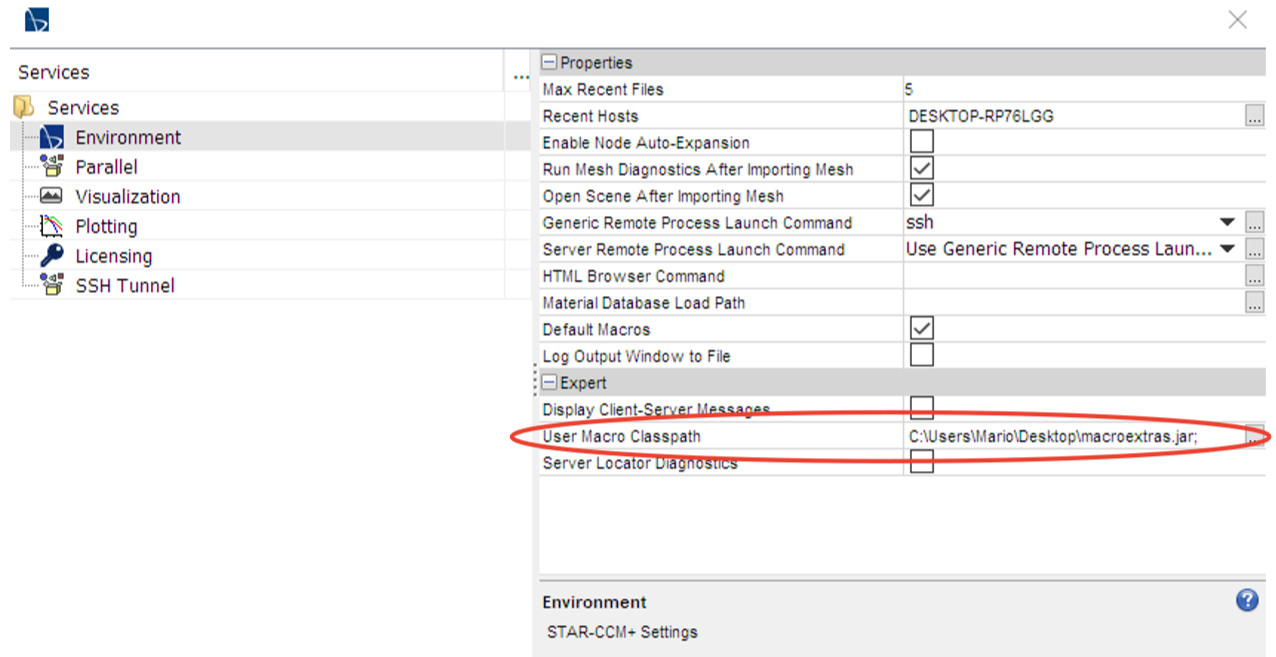
\includegraphics[scale=0.45]{Immagini/Capitolo4/starclasspath2}
\caption{\lstinline[language=Java]!MacroExtras! classpath setting inside STAR-CCM+}
\label{fig:starclasspath}
\end{figure}
%  

\section{Running STAR-CCM+ macros from inside JPAD}
\label{sec4.4}

The classes of the \lstinline[language=Java]!MacroExtras! package listed in the previous paragraph just serve as a support for the Java files in charge of the operations that actually allow to automatize the process of analysis of a certain aircraft configuration by means of a \gls{CFD} tool. The aforementioned Java files are two in number and consist of:
%
\begin{itemize}
\item a simple class providing a main method that imports some aircraft data from XML files, eventually modifies some of the components of the aircraft by means of the methods supplied by \gls{JPAD} libraries, generates a \gls{CAD} file for each of the components employing the functions offered by \lstinline[language=Java]!AircraftUtils!, writes the XML file containing all the data related to the simulation, and finally runs STAR-CCM+;
\item a STAR-CCM+ macro, which is a particular Java class that makes use of the STAR-CCM+ Macro \gls{acr:API} classes, along with the ones described in section \ref{sec4.3}, in order to perform all the operations requested before and after running an aerodynamic simulation, from importing \gls{CAD} parts into the active simulation to saving the simulation once all the calculations have been completed.
\end{itemize}
%
The following paragraphs give an overview on how these two files have been realized and on the methods and classes they make use of. The last one, in particular, just provides an example of how the main method launching the workflow can be organized, since part of its structure depends on the type of experiment/simulation that one wants to perform.

\subsection{The macro}
\label{sec4.4.1}

A STAR-CCM+ macro is a Java program that is compiled and executed within the STAR-CCM+ workspace. In order for STAR-CCM+ to actually run macros, it comes equipped with the Java \gls{acr:SDK} (the 1.7 version, so that Java 8 improvements are not available), that allows the software to compile the Java macros. The macros that one can write or record are standard Java code, meaning that it is possible to have access to all the programming constructs of the language, such as loops and conditional constructs. In addition, the STAR-CCM+ server exposes a certain number of classes, that it is possible to instantiate and manipulate in order to carry out some required sequence of tasks. Macros can be written from scratch, but that would require up-front knowledge about all the classes, attributes, and methods that the server exposes. Instead, it is more effective to use the workspace to record the actions to be performed and edit the Java file using a text editor in order to get the exact required effect.

\bigskip
\noindent
The STAR-CCM+ macro that is currently used in order to perform tests and simulations on \gls{CAD} aircraft parts produced by the use of \gls{JPAD} is called \lstinline[language=Java]!MultipleExecute!. It consists in a sequence of actions, performed in proper order, that allow to simulate fluid flow around the aforementioned aircraft components. As all the STAR-CCM+ macros, it extends the abstract class \lstinline[language=Java]!StarMacro!, and it has been included into a Java project having STAR-CCM+ \gls{JAR}s and class folders on the build path, in order for the STAR-CCM+ macros contained in this package to actually import and use STAR-CCM+ classes. For the same reason, also the path to the \lstinline[language=Java]!MacroExtras! package has been included in the build path. The \lstinline[language=Java]!MultipleExecute! macro consists of several void methods (i.e., methods that do not return anything directly), each one devoted to a specific task, and some attributes, that correspond to variables that can be used by more than one single method during the execution of the macro. As for the global variables, they are the following.
%
\begin{itemize}
\renewcommand\labelitemi{\tiny$\blacksquare$}
\renewcommand\labelitemii{\tiny$\bullet$}
\item \textbf{\lstinline[language=Java]!dataFolderPath!} - A \lstinline[language=Java]!String! variable that stands for the path to the folder in which all the files the simulation needs (the XML data file and the \gls{CAD} files in STEP format) have been stored.
\item \textbf{\lstinline[language=Java]!simFolderPath!} - A \lstinline[language=Java]!String! variable that stores the path to the directory in which the user wants to save the STAR-CCM+ simulation files. Both this and the previous variable need to be fixed by the user, in order for the macro to retrieve and save data in the proper locations.
\item \textbf{\lstinline[language=Java]!theSimulation!} - An instance of the STAR-CCM+ Macro \gls{acr:API} class \lstinline[language=Java]!Simulation!. It is the most important of the global variables of the macro, since it stores all the informations on the active simulation and it is used by all the methods across the class. It gets initialized at the very beginning of the macro, once the launching class has started running the software and played the macro.
\item \textbf{\lstinline[language=Java]!theOperatingConditions!, \lstinline[language=Java]!theGeometricData!, \lstinline[language=Java]!theSimulationParameters!} - Instances of the \lstinline[language=Java]!MacroExtras! classes \lstinline[language=Java]!OperatingConditions!, \lstinline[language=Java]!GeometricData!, and \lstinline[language=Java]!SimulationParameters! respectively. They are the variables devoted to storing all the data coming from the XML input file.
\item \textbf{\lstinline[language=Java]!thePartsMap!} - A \lstinline[language=Java]!HashMap! (an implementation of the Java \gls{Map} interface that permits null values and null keys) having keys of the \lstinline[language=Java]!ComponentEnum! type and Java \gls{List}s of strings as values. It gets initialized by means of the \lstinline[language=Java]!SimulationComponents! getter method \lstinline[language=Java]!getComponentsMap!, so it stores the file paths of each of the components that need to be imported into the active simulation. As the global variables at the previous points, it is initialized at the beginning of the macro, by the first of the methods in which \lstinline[language=Java]!MultipleExecute! macro has been split.
\item \textbf{\lstinline[language=Java]!theAircraftParts!} - A Java \gls{List} containing entities of the STAR-CCM+ \gls{acr:API} class \lstinline[language=Java]!GeometryPart!. This class, in general, manages \gls{CAD} parts once they have been imported into the simulation. So \lstinline[language=Java]!theAircraftParts! is a list containing all the imported aircraft components.
\end{itemize}
%
Listing \ref{lst:MultipleExecuteOverview} shows an overview of the macro, highlighting the attributes and the methods contained in the class. As can be seen from the listing, the macro consists of one main \lstinline[language=Java]!execute! method, which calls all the other methods present in the class in a proper sequence. Since the macro can be used also in a stand-alone way, without launching it from \gls{JPAD} but simply playing it from inside STAR-CCM+, one can think of commenting part of the tasks executed by the code, in order to have a more step-by-step approach. The following sections provide a more detailed description of some of the methods contained in the macro, especially for the ones that make greater use of Java programming constructs.
\bigskip
\begin{lstlisting}[caption={\lstinline!MultipleExecute! macro overview}, captionpos=b, tabsize=2, label={lst:MultipleExecuteOverview}]
public class MultipleExecute extends StarMacro {
	
		// Global variables
		public static final String dataFolderPath = "C:\\Users\\...";
		public static final String simFolderPath = "C:\\Users\\...";
		public static Simulation theSimulation;
		public static OperatingConditions theOperatingConditions;
		public static GeometricData theGeometricData;
		public static SimulationParameters theSimulationParameters;
		public static HashMap<ComponentEnum, List<String>> thePartsMap;
		public static List<GeometryPart> theAircraftParts;

		// Macro main method
		public void execute() {
				initializeSimulation();
				importCadParts();
				createFluidDomain();
				assignPartsToRegion();
				createReferenceValuesReports();
				createDirectionFieldFunctions();
				createMesh();
				physicsSetup();
				createAerodynamicsCoefficients();
				createBoundaryConditions();
				runSimulation();
				saveSimulation();
				killSimulation();
		}
	
		// Macro methods
		public void initializeSimulation() {
		...
		}
	
		...
	
		public void killSimulation() {
		...
		}
}	
\end{lstlisting}

\subsubsection{\texttt{initializeSimulation}}

The first of the macro methods has the fundamental task of populating global variables such as the ones related to the operating conditions, the geometric data, the simulation parameters, and the simulation components \gls{CAD} files. The method filters the files contained in the directory indicated by \lstinline[language=Java]!dataFolderPath!, distinguishing between STEP files and XML data file, and creates two distinct \lstinline[language=Java]!File! arrays, one dedicated to the \gls{CAD} components, the other one for the simulation data. The latter is used by the \lstinline[language=Java]!DataReader! class in order to initialize the global variables: \lstinline[language=Java]!theOperatingConditions!, \lstinline[language=Java]!theGeometricData!, and \lstinline[language=Java]!theSimulationParameters!. The other \lstinline[language=Java]!File! array is used by the \lstinline[language=Java]!SimulationComponents! class in order to generate a \gls{Map} to the files containing all the different \gls{CAD} components (\lstinline[language=Java]!thePartsMap!).

\subsubsection{\texttt{importCADParts}}

Once the paths to the \gls{CAD} files have been collected, it is necessary to import them into the active simulation. The STAR-CCM+ \gls{acr:API} class allowing this is \lstinline[language=Java]!PartImportManager!. Once provided with the path to the actual file and the required options (such as coincidence tolerance, merging options, and tessellation density) it imports the component, which is collected into a Java \gls{List} (\lstinline[language=Java]!theAircraftParts!) after being casted to \lstinline[language=Java]!GeometryPart!. After being imported, it is also possible to set a presentation name for the component and its surfaces, according to the name of the file from which it has been extracted. This is really helpful, since it allows in the following to get from the simulation parts list the desired part just by means of the presentation name set on it at this point. The method also automatically scales the parts according to the value set for the \lstinline[language=Java]!OperatingConditions! \lstinline[language=Java]!cadUnits! attribute. Since the \gls{OCCT} STEP writer class saves shapes in $\si{mm}$ by default, it is necessary to scale them properly.
\bigskip
\begin{lstlisting}[caption={\lstinline!importCADParts! method}, captionpos=b, tabsize=2, label={lst:importCADParts}]
public void importCadParts() {

		LabCoordinateSystem labCoordinateSystem = 
				theSimulation.getCoordinateSystemManager().getLabCoordinateSystem();
		PartImportManager partImportManager = 
				theSimulation.get(PartImportManager.class);

		int partIndex = 0;
		List<GeometryPart> aircraftParts = new ArrayList<>();
		for(Iterator<ComponentEnum> comp = 
				thePartsMap.keySet().iterator(); comp.hasNext(); ) {
			
			// Collect simulation parts into a list	
			ComponentEnum component = comp.next();		
			for(String path : thePartsMap.get(component)) {
				partImportManager.importCadPart(
						resolvePath(path), 
						"SharpEdges", 30.0, 2, true, 1.0E-5, true, false, false, false
						);
				String partName = MyStringUtils.getFilenameFromFilepath(path);
				GeometryPart aircraftPart = 
						((List<GeometryPart>) partImportManager .getParts()).get(partIndex);
				
				// Assign a proper name to the imported part and its surfaces		
				aircraftPart.setPresentationName(partName);
				((List<PartSurface>) aircraftPart.getPartSurfaces())
										.get(0)
										.setPresentationName(partName);
				
				// Scale parts whether necessary
				if(theGeometricData.getCADUnits().equals("mm")) {
					partImportManager.scaleParts(
							Collections.singletonList(aircraftPart), 
							new DoubleVector(new double[] {1000, 1000, 1000}), 
							labCoordinateSystem
							);
				}
				aircraftParts.add(aircraftPart);
				partIndex++;
			}
		}			
		
		// Initialize theAircraftParts global variable
		theAircraftParts = aircraftParts;
	}
\end{lstlisting}

\subsubsection{\texttt{createFluidDomain}}

The next step consists in creating the fluid domain in which the simulation takes place. For this purpose, a new geometry part gets created. This part is a simple block, whose dimensions are automatically set to be multiples of one of the aircraft reference length. In particular, the code set this reference length to be the greatest between the fuselage lenght and the wing span. Besides, depending on the value of the \lstinline[language=Java]!SimulationParameters! \lstinline[language=Java]!isSymmetrical! attribute, the block domain extends from the symmetry plane of the aircraft to both (positive and negative) $y$ directions or just the positive one. In addition, the front extension of the block is set to be lower than the back one, in order to let the fluid settle after having swept the aircraft. Once the block has been created, it's time to split its surface, in order to correctly assign the boundary conditions later in the code. The way the block surface gets split depends on:
%
\begin{itemize}
\item whether the simulation to be performed is symmetrical or not,
\item whether the simulation involves an inviscid flow or not,
\end{itemize}
%
with the latter condition depending on the value of the \lstinline[language=Java]!SimulationParameters! \lstinline[language=Java]!simulationType! attribute. Listing \ref{lst:createFluidDomain01} shows how the block surface gets split and how the different surfaces obtained through the process get named according to the boundary conditions to be applied onto them later. The final operation performed by the method consists in creating the actual fluid domain by means of a Boolean subtraction involving the block and the aircraft parts. The result of this operation is a new geometry part (called simply FLUID) and it is the one that it is actually used in the rest of the macro and on which operations, such as meshing and boundary conditions assignment, are performed. Its surfaces preserve the names assigned, during the previous steps, to the surfaces of the parts that have been used to generate it (i.e., the block domain and the aircraft parts), so that it is easy to retrieve them by means of the same.
\bigskip
\begin{lstlisting}[caption={Fluid domain outer surfaces creation and naming operations}, captionpos=b, tabsize=2, label={lst:createFluidDomain01}]
// Get the block surface in order to split it
PartSurface simpleBlockPartSurfaces = 
		(PartSurface) simpleBlockPart.getPartSurfaceManager()
									.getPartSurface("Block Surface");

// Split the block surface according to the simulation requirements		
if(!theSimulationParameters.isSimulationSymmetrical()) {
		
		// In case the simulation to be performed is not symmetrical
		if(theSimulationParameters.getSimulationType().equals(SimulationType.EULER)) {
		
				// In case of inviscid fluid, the back surface of the fluid block is 
				// named OUTLET, while all the remaining ones are named INLET
				simpleBlockPart.splitPartSurfaceByPatch(
					simpleBlockPartSurfaces, new IntVector(new int[] {6}), "OUTLET");
				simpleBlockPartSurfaces.setPresentationName("INLET");
		} else 
		
				// In case of viscid fluid, all the block surfaces get named FAR-FIELD
				simpleBlockPartSurfaces.setPresentationName("FAR-FIELD");
} else {	
		
		// In case the simulation to be performed is symmetrical
		if(theSimulationParameters.getSimulationType().equals(SimulationType.EULER)) {
		
				// In case of inviscid fluid, the back surface of the fluid block is named
				// OUTLET, the symmetry one is simply named SYMMETRY PLANE, and
				// the remaining ones are named INLET
				simpleBlockPart.splitPartSurfaceByPatch(
					simpleBlockPartSurfaces, new IntVector(new int[] {6}), "OUTLET");
				simpleBlockPart.splitPartSurfaceByPatch(
					simpleBlockPartSurfaces, new IntVector(new int[] {4}), "SYMMETRY PLANE");
				simpleBlockPartSurfaces.setPresentationName("INLET");
		} else {
		
				// In case of viscid fluid, the block symmetry surface is named SYMMETRY
				// PLANE, while the remaining ones are named FAR-FIELD
				simpleBlockPart.splitPartSurfaceByPatch(
					simpleBlockPartSurfaces, new IntVector(new int[] {4}), "SYMMETRY PLANE");
				simpleBlockPartSurfaces.setPresentationName("FAR-FIELD");
		}
}
\end{lstlisting}

\subsubsection{\texttt{createReferenceValuesReports} - \texttt{createDirectionFieldFunctions}}

The \lstinline[language=Java]!createReferenceValuesReports! method generates several instances of the STAR-CCM+ Macro \gls{acr:API} \lstinline[language=Java]!ExpressionReport! class, used to represent constant values that can be used throughout the macro in order to define other reports (such as those relative to aerodynamic coefficients) and to generate user defined field functions. These reports, in particular, get defined by means of the attributes of the simulation data classes \lstinline[language=Java]!OperatingConditions! and \lstinline[language=Java]!GeometricData!, with the latter being used in order to define reference lengths and surfaces. As for the user defined field functions mentioned above, they are produced by the \lstinline[language=Java]!createDirectionFieldFunctions! method and consist in directions that help defining aerodynamic coefficients. In particular, they identify the lift, drag, and side force directions by means of the angle of attack and the sideslip angle specified in the operating conditions. Both the expression reports and the direction field functions are given a specific presentation name, in order to easily retrieve them later by using it. For the sake of completeness, listing \ref{lst:DragDirectionFieldFunction} provides a sample of how direction field functions are created.
\bigskip
\begin{lstlisting}[caption={Drag direction field function}, captionpos=b, tabsize=2, label={lst:DragDirectionFieldFunction}]
// Instantiate a new field function
UserFieldFunction dragDirectionFieldFunction = 
		theSimulation.getFieldFunctionManager().createFieldFunction();
		
// Set the field function to VECTOR type
dragDirectionFieldFunction.getTypeOption()
					.setSelected(FieldFunctionTypeOption.Type.VECTOR);

// Define the direction field function by means of its components, using 
// the expression reports for the angle of attack and the sideslip angle
dragDirectionFieldFunction.setDefinition(
	"[cos(${AngleOfAttack(deg)Report}/57.3)*cos(${SideslipAngle(deg)Report}/57.3)," + 
	"sin(${SideslipAngle(deg)Report}/57.3)," + 
	"sin(${AngleOfAttack(deg)Report}/57.3)*cos(${SideslipAngle(deg)Report}/57.3)]"
	);
		
// Set an appropriate presentation name
dragDirectionFieldFunction.setFunctionName("DragDirection");
dragDirectionFieldFunction.setPresentationName("DragDirection");
\end{lstlisting} 

\subsubsection{\texttt{createMesh}}

The \lstinline[language=Java]!createMesh! method generates the discretized representation of the computational domain, which the physics solvers use to provide a numerical solution. The meshing strategy adopted by the \lstinline[language=Java]!MultipleExecute! macro is parts-based, which is a pretty common strategy for unstructured meshing: it detaches the meshing from the physics and provides a flexible and repeatable meshing pipeline. The first thing the method does is instantiating a new \lstinline[language=Java]!AutoMeshOperation! object, with \lstinline[language=Java]!AutoMeshOperation! being the STAR-CCM+ class that supervises meshing operations. The way this object is instantited depends on the type of simulation to be performed, whether it involves viscid or inviscid fluid flow. So the code contains an \emph{if} statement, whose condition is based on the \lstinline[language=Java]!SimulationParameters! \lstinline[language=Java]!simulationType! attribute. If the type of the simulation has been set to \lstinline[language=Java]!SimulationType.EULER!, the code selects the following options for the \lstinline[language=Java]!AutoMeshOperation! object.
%
\begin{itemize}
\renewcommand\labelitemi{\tiny$\blacksquare$}
\renewcommand\labelitemii{\tiny$\bullet$}
\item \textbf{Surface Remesher} - Remeshes the initial surface to provide a quality discretized mesh that is suitable for \gls{CFD}.
\item \textbf{Automatic Surface Repair} - Provides an automatic procedure for correcting a range of geometric problems that can exist in the remeshed surface once the surface remeshing process is complete.
\item \textbf{Polyhedral Mesher} - Generates a volume mesh that is composed of polyhedral-shaped cells.
\end{itemize} 
%
In addition, when the \lstinline[language=Java]!simulationType! attribute is set to \lstinline[language=Java]!SimulationType.VISCOUS!, the \textbf{Prism Layer Mesher} option gets activated. It adds prismatic cell layers next to wall boundaries, in order to capture viscous gradients at the wall. Once the \lstinline[language=Java]!AutoMeshOperation! object has been created and associated to the fluid domain part generated by the \lstinline[language=Java]!createFluidDomain! method, it is possible to set values for some of its parameters. The macro currently sets values for the following properties.
%
\begin{itemize}
\renewcommand\labelitemi{\tiny$\blacksquare$}
\renewcommand\labelitemii{\tiny$\bullet$}
\item \textbf{Base Size} - A characteristic dimension of the model that can be set before using any relative values. As for the \lstinline[language=Java]!MultipleExecute! macro, this value has been set equal to the greater between the fuselage length and the wing span.
\item \textbf{Growth Factor} - A property that defines the growth of the mesh size, whose value should be set between $1.0$ and $2.0$. Increasing its value results in larger mesh sizes in the transition from boundary size to the size away from the boundary. The macro currently sets its value to $1.3$.
\end{itemize}
%
In case of viscid fluid flow, the macro also automatically sets values regarding the Prism Layer Mesher. In particular, it sets the number of prism layers (currently fixed to $10$) and the absolute prism layer thickness, to calculate the value of which the macro uses the formula for turbulent boundary layers over a flat plate:
\[
\delta \approx 0.37x/{\text{Re}}_{x}^{1/5}
\]
with the Reynolds number based on the reference length expression report created by the \lstinline[language=Java]!createReferenceValuesReports! method (and equal to the wing mean aerodynamic chord). The last operations performed by the method consist in generating custom mesh controls for the aircraft part surfaces  the fluid domain is made up of. In general, surface custom mesh controls override any default controls for the volume mesher, allowing to refine or coarsen the mesh for part surfaces. The custom controls the macro makes use of are the following.
%
\begin{itemize}
\renewcommand\labelitemi{\tiny$\blacksquare$}
\renewcommand\labelitemii{\tiny$\bullet$}
\item \textbf{Target Surface Size} - Defines the edge length that the mesher aims for in absence of any mesh refinement. Decreasing the target surface size generates more refined and detailed surface mesh.
\item \textbf{Minimum Surface Size} - Specifies the lower limit of edge lengths on the surface mesh. Decreasing the minimum surface size allows more refinement in regions where the mesher is trying to capture complex features.
\end{itemize}
% 
The \lstinline[language=Java]!MultipleExecute! macro specifies the controls listed above for each aircraft surface and as relative to the aforementioned base size. Besides, the code automatically detects the type of the surface the controls are being set for, and uses different values depending on which part surfaces belong to. For example, the values used for the fuselage are five times the ones used for the lifting surfaces in general (target surface size equal to $0.1$ of the base size, minimum surface size equal to $0.01$ of the base size), since the latter typically require much more mesh refinement.
%
\bigskip
\begin{figure}[H]
\centering
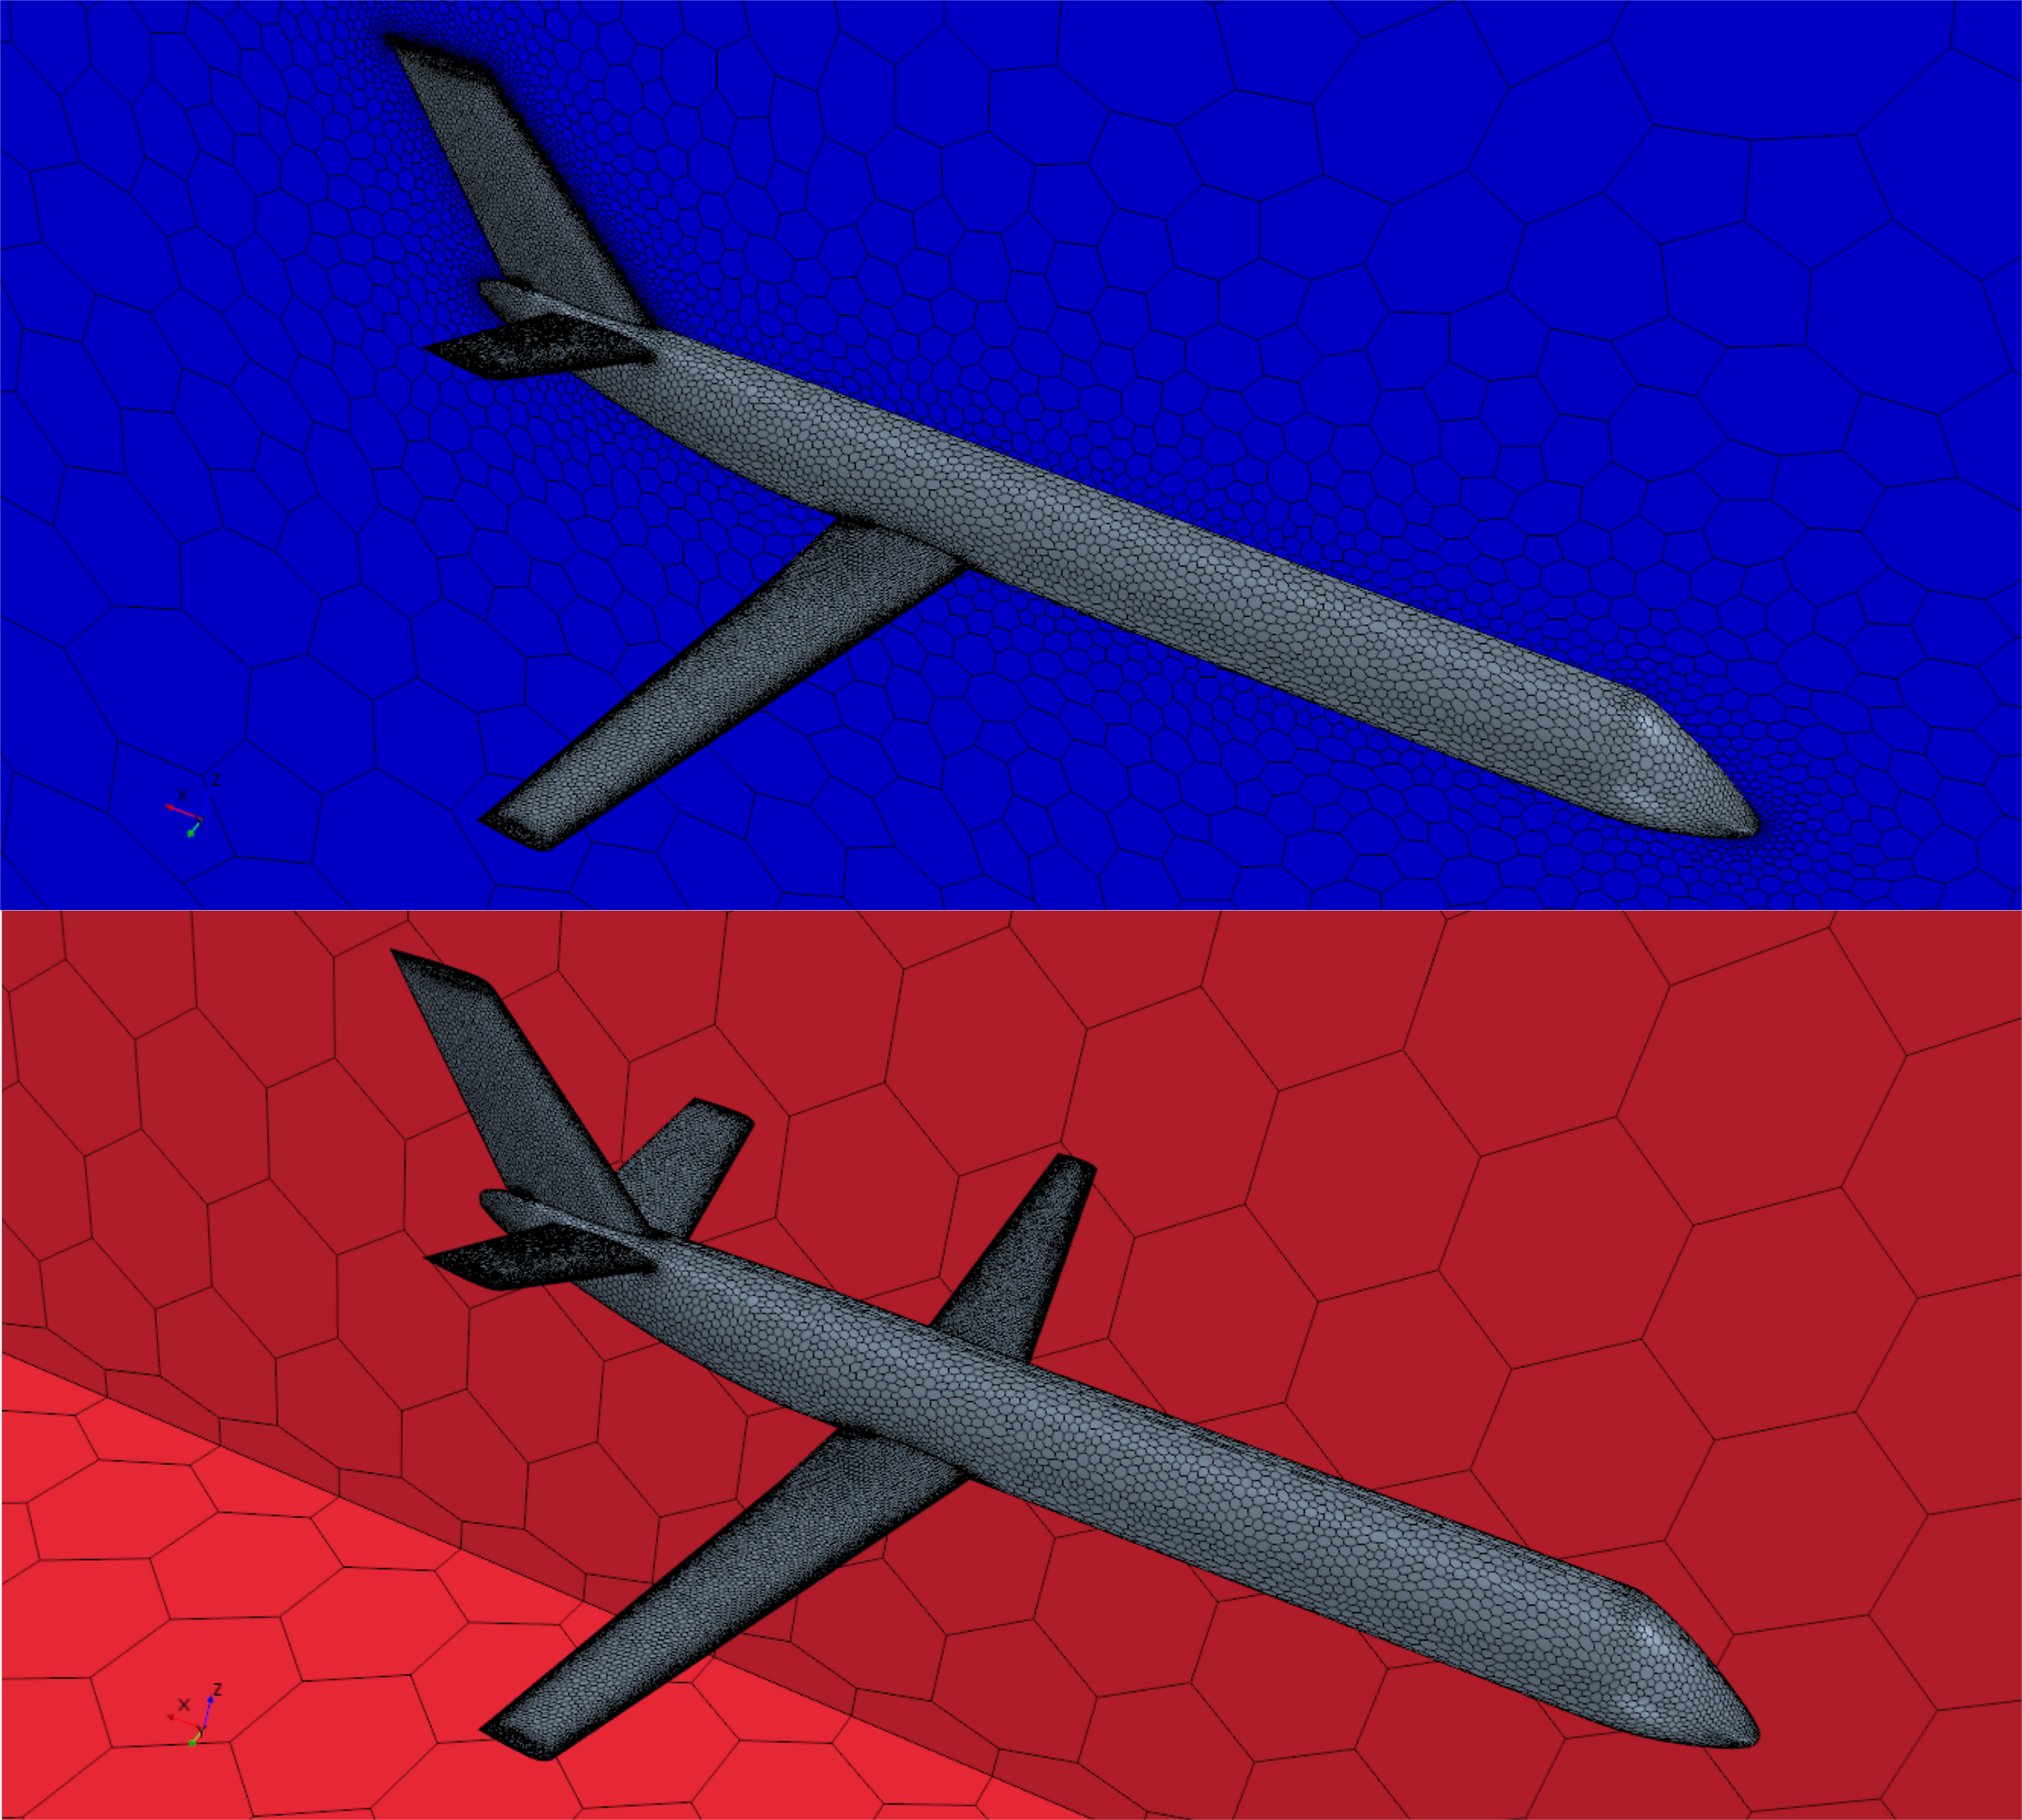
\includegraphics[scale=0.60]{Immagini/Capitolo4/symmetry}
\caption{Automated meshes for symmetrical/non-symmetrical simulations}
\label{fig:SymmMesh}
\end{figure} 
%
\begin{figure}[H]
\centering
\includegraphics[scale=0.60]{Immagini/Capitolo4/airfoil}
\caption{Automated meshes for non-viscous/viscous fluid flows}
\label{fig:AirfoilMesh}
\end{figure} 
%

\subsubsection{\texttt{physicsSetup}}

Once the meshing operations have been defined (altough the actual mesh still needs to be generated), the macro arranges for the set up of the physics models. These define the primary variables of the simulation and what mathematical formulation is used to generate the solution. An appropriate combination of models is necessary for the complete definition of a physics continuum. After generating a new \lstinline[language=Java]!PhysicsContinuum! object, with \lstinline[language=Java]!PhysicsContinuum! being the class that manages physics models definition, the method enables several physics models, common to both viscid and inviscid flow simulations. Then an \emph{if} statement allows to select different models depending on the value of the \lstinline[language=Java]!SimulationParameters! \lstinline[language=Java]!simulationType! attribute. In case the attribute is equal to \lstinline[language=Java]!SimulationType.EULER!, the Inviscid Model is enabled. If not, several models relative to turbulence and its treatment get implemented. Listing \ref{lst:PhysicsSetup} reports the whole method, along with the list of physics models enabled by the macro.
\bigskip
\begin{lstlisting}[caption={\lstinline!physicsSetup! method}, captionpos=b, tabsize=2, label={lst:PhysicsSetup}]
public void physicsSetup() {

		// Generate a new instance of PhysicsContinuum
		PhysicsContinuum physicsContinuum = 
				theSimulation.getContinuumManager().createContinuum(PhysicsContinuum.class);
		physicsContinuum.setPresentationName("Physics");
		
		// Enable some basic physics models
		physicsContinuum.enable(ThreeDimensionalModel.class);
		physicsContinuum.enable(SteadyModel.class);
		physicsContinuum.enable(SingleComponentGasModel.class);
		physicsContinuum.enable(CoupledFlowModel.class);
		physicsContinuum.enable(IdealGasModel.class);
		physicsContinuum.enable(CoupledEnergyModel.class);
		
		// Enable more specific physics models
		if(theSimulationParameters.getSimulationType().equals(SimulationType.VISCOUS)) {
			physicsContinuum.enable(TurbulentModel.class);
			physicsContinuum.enable(RansTurbulenceModel.class);
			physicsContinuum.enable(SpalartAllmarasTurbulence.class);
			physicsContinuum.enable(SaTurbModel.class);
			physicsContinuum.enable(SaAllYplusWallTreatment.class);
		} else {
			physicsContinuum.enable(InviscidModel.class);
		}	
		
		// Set a value for the reference pressure
		physicsContinuum.getReferenceValues()
					.get(ReferencePressure.class)
					.setValue(theOperatingConditions.getPressure());
}
\end{lstlisting}  

\subsubsection{\texttt{createAerodynamicsCoefficients}}

The expression reports and the direction field functions created by the methods described above are mostly used in order to define aerodynamic coefficients. \lstinline[language=Java]!ForceCoefficientReport! and \lstinline[language=Java]!MomentCoefficientReport! are the STAR-CCM+ classes that help creating this kind of entities. These coefficients, in order to be properly defined, need to be associated to the surfaces on which they are calculated. All the coefficients defined at this point are calculated on the whole aircraft. Listing \ref{lst:createAerodynamicsCoefficients} shows how the lift coefficient and the pitch moment coefficient reports are defined. It has to be noted that the reference surface area gets automatically adjusted in case the simulation to be performed is symmetrical. In addition to the reports for the aerodynamic coefficients, the method also provides the definitions for the pressure coefficient (by means of the \lstinline[language=Java]!PressureCoefficientFunction! class) and, in case \lstinline[language=Java]!simulationType! is set to \lstinline[language=Java]!VISCOUS!, the skin friction coefficient (by means of the \lstinline[language=Java]!SkinFrictionCoefficientFunction! class).
\bigskip
\begin{lstlisting}[caption={Force and moment coefficients creation}, captionpos=b, tabsize=2, label={lst:createAerodynamicsCoefficients}]
// Generate a new force coefficient instance
ForceCoefficientReport liftCoefficientReport 
		= theSimulation.getReportManager().createReport(ForceCoefficientReport.class);
		
// Set a direction by means of the field function created before	
liftCoefficientReport.getDirection().setDefinition("$${LiftDirection}");

// Set reference quantities by means of the expression reports created above
liftCoefficientReport.getReferenceDensity().setDefinition(
		"${DensityReport}");
liftCoefficientReport.getReferenceVelocity().setDefinition(
		"${ReferenceVelocityReport}");
liftCoefficientReport.getReferenceArea().setDefinition(
		"${ReferenceAreaReport}/" + Integer.toString(symmetryFactor));

// Set the surface
liftCoefficientReport.getParts().setObjects(aircraftBoundaries);

// Set the presentation name
liftCoefficientReport.setPresentationName("CL");

// Generate a new moment coefficient instance
MomentCoefficientReport pitchMomentCoefficientReport = 
		theSimulation.getReportManager().createReport(MomentCoefficientReport.class);

// Set a direction by using components		
pitchMomentCoefficientReport.getDirection().setComponents(0.0, 1.0, 0.0);

// Set reference quantities by means of the expression reports created above
pitchMomentCoefficientReport.getReferenceDensity().setDefinition(
		"${DensityReport}");
pitchMomentCoefficientReport.getReferenceVelocity().setDefinition(
		"${ReferenceVelocityReport}");
pitchMomentCoefficientReport.getReferenceRadius().setDefinition(
		"${ReferenceLengthReport}");
pitchMomentCoefficientReport.getReferenceArea().setDefinition(
		"${ReferenceAreaReport}/" + Integer.toString(symmetryFactor));

// Set the pole
pitchMomentCoefficientReport.getOrigin().setDefinition(
		"[${ReferenceMomentPoleReport}, 0.0, 0.0]");

// Set the surface
pitchMomentCoefficientReport.getParts().setObjects(aircraftBoundaries);

// Set the presentation name
pitchMomentCoefficientReport.setPresentationName("CM");
\end{lstlisting}

\subsubsection{\texttt{createBoundaryConditions}}

Before finally being able to run the simulation, boundary conditions must be applied. Since the fluid domain surface has already been split by one of the previous methods, at this point it's just necessary to impose proper conditions, based on the name given to the surfaces by the same method. For this purpose, \lstinline[language=Java]!createBoundaryConditions! performs a first check on the symmetry of the problem: if so, a symmetry boundary condition is applied on the fluid domain surface previously named SYMMETRY PLANE (listing \ref{lst:createFluidDomain01}). Then, an \emph{if} statement, whose condition depends on the \lstinline[language=Java]!simulationType! attribute, helps the code deciding which boundary conditions should be applied on the remaining surfaces. If the simulation to be performed involves inviscid fluid, velocity inlet and pressure outlet boundary conditions are applied on the surfaces previously named INLET and OUTLET respectively. Otherwise, a free-stream condition is applied on the FAR-FIELD surfaces of the fluid domain. As for the aircraft surfaces, a wall boundary condition is applied automatically, so there's no need to modify anything. In order to set values for the quantities that it is necessary to define for each of the boundary conditions mentioned above, expression reports and direction field functions are used. Listing \ref{lst:CreateBoundaryConditions} shows the entire method, along with the quantities defined for the boundary conditions.
\bigskip
\begin{lstlisting}[caption={\lstinline!createBoundaryConditions! method}, captionpos=b, tabsize=2, label={lst:CreateBoundaryConditions}]
public void createBoundaryConditions() {
	
	// Instantiate a new BoundaryManager object
	BoundaryManager boundaryManager 
			= theSimulation.getRegionManager().getRegion("Region").getBoundaryManager();

	// Checking on symmetry		
	if(theSimulationParameters.isSimulationSymmetrical()) {
	
		// Get the symmetry surface by means of its 
		// presentation name and set its boundary type
		boundaryManager.getBoundary("FLUID.Block.SYMMETRY PLANE")
			.setBoundaryType(
				(SymmetryBoundary) theSimulation.get(ConditionTypeManager.class)
									.get(SymmetryBoundary.class));
	}
		
	// Simulation type check	
	if(theSimulationParameters.getSimulationType().equals(SimulationType.EULER)) {
	
		// In case of inviscid fluid flow		
		Boundary inflow = boundaryManager.getBoundary("FLUID.Block.INLET");
		Boundary outflow = boundaryManager.getBoundary("FLUID.Block.OUTLET");

		inflow.setBoundaryType(
			(InletBoundary) theSimulation.get(ConditionTypeManager.class)
									.get(InletBoundary.class));		
		outflow.setBoundaryType(
			(PressureBoundary) theSimulation.get(ConditionTypeManager.class)
									.get(PressureBoundary.class));
									
		// Set definitions for velocity inlet BC quantities
		inflow.getConditions().get(FlowDirectionOption.class)
						.setSelected(FlowDirectionOption.Type.COMPONENTS);
		inflow.getValues().get(FlowDirectionProfile.class)
						.getMethod(ConstantVectorProfileMethod.class)
						.getQuantity().setDefinition("$${DragDirection}");
		inflow.getValues().get(StaticTemperatureProfile.class)
						.getMethod(ConstantScalarProfileMethod.class)
						.getQuantity().setDefinition("${TemperatureReport}");
		inflow.getValues().get(VelocityMagnitudeProfile.class)
						.getMethod(ConstantScalarProfileMethod.class)
						.getQuantity().setDefinition("${ReferenceVelocityReport}");
		
		// Set definitions for pressure outlet BC quantities
		outflow.getValues().get(StaticTemperatureProfile.class)
						.getMethod(ConstantScalarProfileMethod.class)
						.getQuantity().setDefinition("${TemperatureReport}");
	} else {
	
		// In case of viscous fluid flow
		Boundary freeStream = boundaryManager.getBoundary("FLUID.Block.FAR-FIELD");

		freeStream.setBoundaryType(
			(FreeStreamBoundary) theSimulation.get(ConditionTypeManager.class)
									.get(FreeStreamBoundary.class));
		
		// Set definitions for free-stream BC quantities
		freeStream.getValues().get(FlowDirectionProfile.class)
						.getMethod(ConstantVectorProfileMethod.class)
						.getQuantity().setDefinition("$${DragDirection}");
		freeStream.getValues().get(MachNumberProfile.class)
						.getMethod(ConstantScalarProfileMethod.class)
						.getQuantity().setDefinition("${MachNumberReport}");
		freeStream.getValues().get(StaticTemperatureProfile.class)
						.getMethod(ConstantScalarProfileMethod.class)
						.getQuantity().setDefinition("${TemperatureReport}");
	}
}
\end{lstlisting}

\subsubsection{\texttt{runSimulation} - \texttt{saveSimulation} - \texttt{killSimulation}}

The three last methods allow, respectively, to generate the mesh and run the simulation (whether the \lstinline[language=Java]!executeMesh! attribute has been set to \lstinline[language=Java]!TRUE!), to save the simulation with a proper name, and to kill the simulation. The last step is fundamental when playing the macro in batch mode, because it allows to properly close the active simulation, in order to start a new one or simply end the process.

\subsection{The launching class}
\label{sec4.4.2}

The last piece of the puzzle consists of the Java class which, equipped with a main method and a series of attributes used as global variables, allows to launch a simulation (or a cycle of simulations) from within \gls{JPAD}. It is necessary to point out that the class described below provides only an example of how the main method should be structured for simulation purposes. In particular, the class described in the following corresponds to the one used for testing out the macro described in the previous paragraph and the system of classes provided by \lstinline[language=Java]!MacroExtras!. 

\bigskip
\noindent
First thing, the launching class requires some attributes to be set. These attributes, corresponding to instances of the Java \lstinline[language=Java]!String! class, are the following.
%
\begin{itemize}
\renewcommand\labelitemi{\tiny$\blacksquare$}
\item \textbf{\lstinline[language=Java]!workingFolderPath!} - Defines the path to the folder in which \gls{CAD} files are stored, along with the XML file containing all the information about the simulation to be run.
\item \textbf{\lstinline[language=Java]!jpadCADFolder!} - Defines the path to the folder in which \gls{JPAD} \gls{CAD} files are generated and initially stored.
\item \textbf{\lstinline[language=Java]!macroPath!} - Contains the path of the folder in which the custom macros are stored (\lstinline[language=Java]!MultipleExecute! is one of them).
\item \textbf{\lstinline[language=Java]!macroName!} - A string standing for the name of the macro to be run.
\item \textbf{\lstinline[language=Java]!starExePath!} - Defines the path to the STAR-CCM+ .exe file.
\item \textbf{\lstinline[language=Java]!starOptions!} - A Java \lstinline[language=Java]!String! containing a set of option for STAR-CCM+ execution, like the path to the software license and the number of processors that must be used during the simulation.
\end{itemize}
%
As for the main method of the class, the first operation performed consists in loading an aircraft from XML data file. For this purpose, the \lstinline[language=Java]!AircraftUtils.importAircraft! method is used, once the launching class run configuration has been provided with an appropiate set of arguments (see section \ref{sec3.6}). After the aircraft has been correctly imported, what the code makes is building a \gls{Map}, called \lstinline[language=Java]!aeroMap!, similar to the one produced by the \lstinline[language=Java]!SimulationComponents! class: it contains \lstinline[language=Java]!MacroExtras! \lstinline[language=Java]!ComponentEnum! constants as keys to Java \gls{List}s of generic objects, which can be instances of \gls{JPAD} \lstinline[language=Java]!Fuselage! and \lstinline[language=Java]!LiftingSurface! classes. The actual \gls{Map} implementation used in the code is the \lstinline[language=Java]!ConcurrentHashMap!, which allows concurrent modification of the \gls{Map} and allows it to be modified during iteration. Listing \ref{lst:AeroMap} shows how this \gls{Map} is created. It is important to note that each key is associated to a list and not to just a single entity, in accordance with the way in which the \lstinline[language=Java]!MacroExtras! classes and the \lstinline[language=Java]!MultipleExecute! macro have been arranged. This means that, for example, one can think of chosing one of the aircraft components present in \lstinline[language=Java]!aeroMap!, generate a copy of the original one and modify it by means of the methods offered by the \gls{JPAD} library, and finally add it to \lstinline[language=Java]!aeroMap!, as listing \ref{lst:AddCustomComponents} shows.
%
\bigskip
\begin{lstlisting}[caption={Aircraft Map creation}, captionpos=b, tabsize=2, label={lst:AeroMap}]
// Import aircraft data from file
Aircraft aircraft = AircraftUtils.importAircraft(args);	

// Generate the Map and populate it with keys 
// and empty Lists of generic Java Object entities	
ConcurrentHashMap<ComponentEnum, List<Object>> aeroMap 
		= new ConcurrentHashMap<ComponentEnum, List<Object>>();
aeroMap.put(ComponentEnum.FUSELAGE, new ArrayList<Object>());
aeroMap.put(ComponentEnum.WING, new ArrayList<Object>());
aeroMap.put(ComponentEnum.CANARD, new ArrayList<Object>());
aeroMap.put(ComponentEnum.HORIZONTAL, new ArrayList<Object>());
aeroMap.put(ComponentEnum.VERTICAL, new ArrayList<Object>());

// Iterate through the Map, adding Fuselage and LiftingSurface  
// objects to the initially empty Lists whether necessary			
for(Iterator<ComponentEnum> comp = aeroMap.keySet().iterator(); comp.hasNext(); ) {
			
	ComponentEnum component = comp.next();
	switch(component) {
	
	// Add fuselages to the Map		
	case FUSELAGE:
		if(!(aircraft.getFuselage() == null))
			aeroMap.get(ComponentEnum.FUSELAGE).add(aircraft.getFuselage());
		else {
			System.out.println("There's no FUSELAGE component for the selected aircraft");
			aeroMap.remove(component);
		}
				
		break;
	
	// Add wings to the Map			
	case WING:
		if(!(aircraft.getWing() == null))
			aeroMap.get(ComponentEnum.WING).add(aircraft.getWing());
		else {
			System.out.println("There's no WING component for the selected aircraft");
			aeroMap.remove(component);
		}
				
		break;
				
	...
	}
}
\end{lstlisting}
%
\bigskip
\begin{lstlisting}[caption={Adding custom components to the original Map}, captionpos=b, tabsize=2, label={lst:AddCustomComponents}]
// Chose to add a custom canard, if the original aircraft has one
ComponentEnum customComponentEnum = ComponentEnum.CANARD;
if(aeroMap.containsKey(customComponentEnum)) {
		
	// Return in case it has been decided to add a custom fuselage	
	if(customComponentEnum.equals(ComponentEnum.FUSELAGE)) return;
	
	// Initialize the original component and the custom component		
	LiftingSurface originalComponent = (LiftingSurface) aeroMap
											.get(customComponentEnum).get(0);
	LiftingSurface customComponent = null;
	
	// Reimport the component to be modified		
	switch(customComponentEnum.name()) {
			
	case "WING": 
		customComponent = AircraftUtils.importAircraft(args).getWing();
		break;
						
	...

	}
	
	// Modify the chosen component by means of JPAD methods and criteria				
	customComponent.adjustDimensions(
			originalComponent
					.getAspectRatio()*1.2,
			originalComponent.getEquivalentWing().getPanels().get(0)
					.getChordRoot().doubleValue(SI.METER)*1.1,
			originalComponent.getEquivalentWing().getPanels().get(0)
					.getChordTip().doubleValue(SI.METER)*0.9, 
			originalComponent.getEquivalentWing().getPanels().get(0)
					.getSweepLeadingEdge(),
			originalComponent.getEquivalentWing().getPanels().get(0)
					.getDihedral(), 
			originalComponent.getEquivalentWing().getPanels().get(0)
					.getTwistGeometricAtTip(), 
			WingAdjustCriteriaEnum.AR_ROOTCHORD_TIPCHORD
			);
	
	// Set the airfoil list for the custom component		
	customComponent.setAirfoilList(originalComponent.getAirfoilList());	
	
	// Set the coordinates for the construction axes origin of the custom component
	customComponent.setXApexConstructionAxes(
			originalComponent.getXApexConstructionAxes()
			.plus(Amount.valueOf(3, SI.METER)));
	customComponent.setYApexConstructionAxes(
			originalComponent.getYApexConstructionAxes());
	customComponent.setZApexConstructionAxes(
			originalComponent.getZApexConstructionAxes()
			.plus(Amount.valueOf(0.1, SI.METER)));
	
	// Finally add the custom component to the Map
	aeroMap.get(customComponentEnum).add(customComponent);
}
\end{lstlisting}
%

\bigskip
\noindent
Once all has been set on the aircraft components side, it's necessary to fix the simulation data by means of the classes provided by \lstinline[language=Java]!MacroExtras!. For this purpose, three new instances of the classes listed in section \ref{sec4.3.2} are created. As for the geometric data, the getter methods provided by the \lstinline[language=Java]!Fuselage! and \lstinline[language=Java]!LiftingSurface! classes are used. Besides, a check is made on the components contained in the aircraft \gls{Map}: if no fuselage is present, the fuselage length attribute of the \lstinline[language=Java]!GeometricData! class is automatically set to zero (so that the macro showed in the previous paragraph always choses the wing span as the reference length), while if no wing is present among the keys list of \lstinline[language=Java]!aeroMap! the code flow is stopped and the main method of the STAR-CCM+ macro launching class returns nothing. As for the operating conditions, instead, the launching class makes use of two of \gls{JPAD} utility classes, \lstinline[language=Java]!AtmosphCalc! and \lstinline[language=Java]!StdAtmos1976!, which provide methods for calculating the atmospheric properties of the \gls{acr:ICAO} 1976 Standard Atmosphere to an arbitrary altitude. Once everything is ready, the builders of the simulation data classes provide the methods to be used in order to generate the objects to be passed to the \lstinline[language=Java]!DataWriter! class (listing \ref{lst:OperCond01} and \ref{lst:DatWrit01}).
%
\bigskip
\begin{lstlisting}[caption={Instantiate a new \lstinline!OperatingConditions! object}, captionpos=b, tabsize=2, label={lst:OperCond01}]
// Define the operating conditions
double angleOfAttack = 2.0;
double sideslipAngle = 0.0;
double machNumber = 0.64;
double altitude = 30000; 
double altitudeM = Amount.valueOf(altitude, NonSI.FOOT)
						.doubleValue(SI.METER);
		
StdAtmos1976 atmosphere = AtmosphereCalc.getAtmosphere(altitudeM);
double pressure = atmosphere.getPressure();
double density = atmosphere.getDensity()*1000;
double temperature = atmosphere.getTemperature();
double speedOfSound = atmosphere.getSpeedOfSound();
double dynamicViscosity = AtmosphereCalc.getDynamicViscosity(altitudeM);
double velocity = speedOfSound*machNumber;
double reynoldsNumber = density*velocity*wingMAC/dynamicViscosity;

// Generate the operating conditions object
OperatingConditions operatingConditions = 
		new OperatingConditions.OperatingConditionsBuilder()
				.setAngleOfAttack(angleOfAttack)
				.setSideslipAngle(sideslipAngle)
				...
				.setVelocity(velocity)
				.build();
\end{lstlisting}
%
\bigskip
\begin{lstlisting}[caption={Instantiate a new \lstinline!DataWriter! object}, captionpos=b, tabsize=2, label={lst:DatWrit01}]
// Create the data file writer
DataWriter writer = new DataWriter(
		operatingConditions, 
		geometricData, 
		simulationParameters			
		);
\end{lstlisting}
%

\bigskip
\noindent
The XML data file is not the only file that the launching class needs to generate. By means of the utilities listed in Chapter \ref{chap3}, it also generates the \gls{CAD} files, in STEP format, containing the solid counterparts of the components listed in \lstinline[language=Java]!aeroMap!. What the launching class does, in particular, is to iterate through the keys of the aircraft components \gls{Map}, chosing for each key the right method and the proper options to be set for it, depending on the type of the component to be converted to \gls{CAD} file. Listing \ref{lst:AircraftCADFiles} shows an excerpt of the original code in which the operations just described are performed. It has to be noted that also the name each file is given is chosen precisely, because from it depends the right functioning of the macro, as described in the previous paragraph.
%
\bigskip
\begin{lstlisting}[caption={Aircraft components CAD files generation}, captionpos=b, tabsize=2, label={lst:AircraftCADFiles}]
// Create aircraft CAD files
List<String> cadNames = new ArrayList<>();
		
// Iterate through aircraft components Map keys
for(Iterator<ComponentEnum> comp = aeroMap.keySet().iterator(); comp.hasNext(); ) {
	ComponentEnum component = comp.next();
			
	switch(component.name()) {
	
	// Transfer fuselage shapes to CAD file		
	case "FUSELAGE":
		int nFus = aeroMap.get(component).size();				 
		for(int i = 0; i < nFus; i++) {
			String cadName = (nFus > 1) ? ("FUSELAGE_" + (i + 1)) : "FUSELAGE";
			cadNames.add(cadName);
			AircraftUtils.getAircraftSolidFile(
				AircraftUtils.getFuselageCAD(
					(Fuselage) aeroMap.get(component).get(i), 
					7, 7, true, true, false), 
				cadName, 
				FileExtension.STEP);
		}
		break;
	
	// Transfer wing shapes to CAD file			
	case "WING":
		int nWng = aeroMap.get(component).size();				 
		for(int i = 0; i < nWng; i++) {
			String cadName = (nWng > 1) ? ("WING_" + (i + 1)) : "WING";
			cadNames.add(cadName);
			AircraftUtils.getAircraftSolidFile(
				AircraftUtils.getLiftingSurfaceCAD(
					(LiftingSurface) aeroMap.get(component).get(i), 
					ComponentEnum.WING, 1e-3, false, true, false), 
				cadName, 
				FileExtension.STEP);
		}
		break;				
	...
}
\end{lstlisting}
%

\bigskip
\noindent
At this point, all the necessary preparations for the launch of the macro are almost over. What remains to be done is to make copies of the \gls{CAD} files generated at the previous step and move them to the folder in which all the simulation files are stored (\lstinline[language=Java]!workingFolderPath!). Besides, it is necessary to actually write to XML file format the simulation data. This operation can be performed by using the \lstinline[language=Java]!write! method supplied by the \lstinline[language=Java]!DataWriter! class. Finally, the macro can be played by running the STAR-CCM+ application in batch mode. The Java classes allowing this are \lstinline[language=Java]!Runtime! and \lstinline[language=Java]!Process!. By means of the former the application (i.e., the launching class) is allowed to interface with the environment in which it is running. The \lstinline[language=Java]!getRuntime! method of this class simply returns the runtime object associated with the current Java application, which can be used in order to execute commands provided to the \lstinline[language=Java]!Runtime! class \lstinline[language=Java]!exec! method in the form of strings. The usage of this method produces an instance of the \lstinline[language=Java]!Process! class, which allows to perform input from the process, perform output to the process, wait for the process to complete, check the exit status of the process, and destroy (kill) the process. Listing \ref{lst:RunningSTAR} shows precisely how the procedure described above has been coded.
%
\bigskip
\begin{lstlisting}[caption={Launching class final steps}, captionpos=b, tabsize=2, label={lst:RunningSTAR}]
// Copy the CAD files and move them to the working folder
cadNames.forEach(s -> {
	try { 
		Files.copy(		
			Paths.get(jpadCADFolder + "\\" + s + ".step"), 
			Paths.get(workingFolderPath + "\\" + s + ".step"), 
			StandardCopyOption.REPLACE_EXISTING
			);
	} 
	catch (IOException e) {
		e.printStackTrace();
	}
});

// Write simulation data to XML file format		
writer.write(workingFolderPath + "\\Data.xml");
		
// Run STAR-CCM+ application in batch mode 
// and play MultipleExecute Java macro
try {
	// Get the runtime object
	Runtime runtime = Runtime.getRuntime();
		
	// Execute commands	
	Process runTheMacro = runtime.exec(
		"cmd /c cd\\ && cd " + macroPath + " && dir && " + // change directory
		"\"" + starExePath + "\" " +  // run the application
		starOptions + " " +  // set license and settings
		"-new -batch " + macroName // start new simulation in batch mode
		); 
	
	// Get the input from the running process and print it to console		         
	BufferedReader input = 
		new BufferedReader(new InputStreamReader(runTheMacro.getInputStream()));
            
        String line = null;		
	while((line = input.readLine()) != null) System.out.println(line);
		
	// Exit the process once all the operations prescribed  
	// by the previous step have been completed	
	int exitVal = runTheMacro.waitFor();
        System.out.println("Exited with error code " + exitVal);
}
		
catch(Exception e) {
	System.out.println(e.toString());
	e.printStackTrace();
}
\end{lstlisting}
%

\bigskip
\noindent
The steps listed above show how to launch a single simulation starting from a dedicated class contained in \gls{JPAD}, making use of the \lstinline[language=Java]!MacroExtras! classes and a STAR-CCM+ macro specifically written for the purpose. At this point it is immediate to think that such an operation can be launched several times consecutively, employing the loop statements offered by the Java language, for the purpose of, for example, studying the contribution to the aerodynamics of the aircraft offered by lifting surfaces with different characteristics or simply positioned in an alternative manner (and it has been seen right above, listing \ref{lst:AddCustomComponents}, how the \lstinline[language=Java]!Fuselage! and \lstinline[language=Java]!LiftingSurface! classes through their methods easily allow to act on aircraft components parameters). Figure \ref{fig:STARJPADWorkflow} summarizes these concepts, offering an overview of how a workflow involving the \gls{JPAD} library and the STAR-CCM+ analysis tools could be arranged.
%
\begin{figure}[H]
\centering
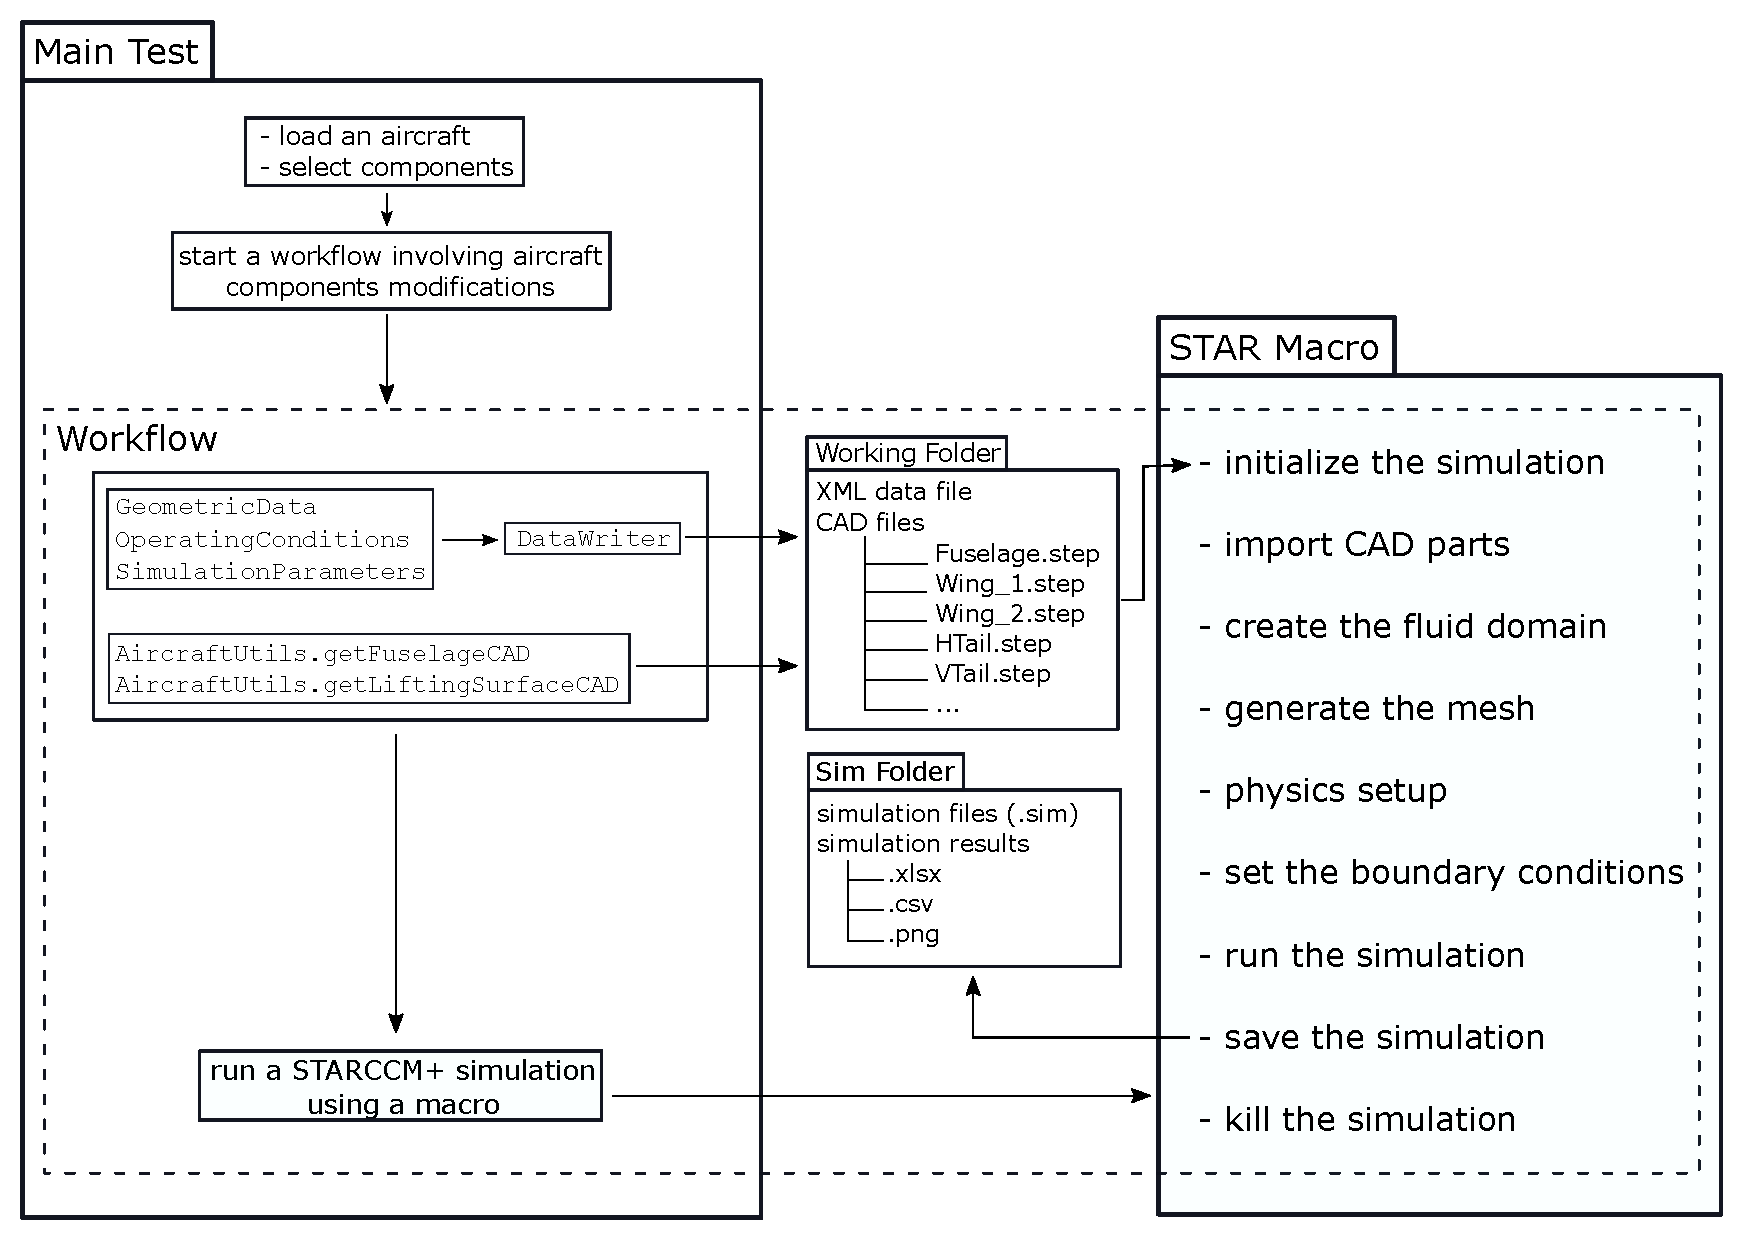
\includegraphics[scale=0.50]{Immagini/Capitolo4/starworkflow}
\caption{JPAD - STAR-CCM+ workflow overview}
\label{fig:STARJPADWorkflow}
\end{figure}
%  

\subsection{Interoperability example}
\label{sec4.4.3}

The following tables and pictures show an example of usage of the framework described in this chapter. The simulations (involving an inviscid fluid flow) have been performed on an innovative configuration developed by the DAF research group as part of the IRON Project. The code explained in the previous chapter has been used in order to modify the aircraft configuration. More in general, \gls{CFD} analyses performed on \gls{CAD} components generated by means of \lstinline[language=Java]!JPADCAD! and \lstinline[language=Java]!AircraftUtils! have returned plausible results, and in accordance with the ones obtained for more refined \gls{CAD} models. However, still more tests are needed in this sense, especially for simulations involving viscous flow.
%
\bigskip
\begin{table}[H]
\centering
\begin{tabular}{lr}
\toprule
\multicolumn{2}{c}{\textbf{Operating Conditions}} \\
\midrule
$\alpha$ & $\SI{2}{\degree}$ \\
$\beta$ & $\SI{0}{\degree}$ \\
$\text{M}$ & $0.64$\\
$h$ & $\SI{30000}{\foot}$ \\
$V$ & $\SI{194.07}{\meter\per\second}$ \\
\bottomrule
\end{tabular}
\caption{Operating conditions for both the tests}
\label{tab:Operating_Conditions}
\end{table}
%
\begingroup
\begin{longtable}[h]{lr}
\textbf{} & \textbf{Geometric data} \\
\toprule
\endfirsthead
%
\multicolumn{2}{l}%
  {\relsize{-1}({\itshape continued from previous page})}\\
 \textbf{} & \textbf{Geometric data} \\
\toprule
\endhead
%
\midrule \multicolumn{2}{r}{{\relsize{-1}\itshape continued on next page}}
\endfoot
%
\bottomrule
\caption{Aircraft data}
\endlastfoot
%
\textbf{Fuselage} & \textbf{ } \\
\midrule
Total Length & $\SI{38.04}{\meter}$ \\
Cylinder Diameter & $\SI{3.510}{\meter}$ \\
\midrule
\textbf{Wing} & \textbf{ } \\
\midrule
Planform Surface & $\SI{98.6}{\square\meter}$ \\
\AR & 11.96 \\
Span & $\SI{34.34}{\meter}$ \\
Mean Aerodynamic Chord & $\SI{3.05}{\meter}$ \\
Twist at Root & $\SI{0.0}{\degree}$ \\
Twist at Tip & $\SI{-2.0}{\degree}$ \\
\midrule
\textbf{Horizontal Tail} & \textbf{ } \\
\midrule
Planform Surface & $\SI{39.91}{\square\meter}$ \\
\AR & 4.261 \\
Span & $\SI{13.04}{\meter}$ \\
\midrule
\textbf{Vertical Tail} & \textbf{ } \\
\midrule
Planform Surface & $\SI{24.45}{\square\meter}$ \\
\AR &  1.366 \\
Span & $\SI{5.78}{\meter}$ \\
\midrule
\textbf{Canard} & \textbf{ } \\
\midrule
Planform Surface & $\SI{10.974}{\square\meter}$ \\
\AR &  5.125 \\
Span & $\SI{7.5}{\meter}$ \\
\end{longtable}
\endgroup
%
\bigskip
\begin{table}[H]
\centering
\begin{tabular}{lrrr}
\toprule
\textbf{Part} & \textbf{$C_{L}$} & \textbf{$C_{D}$} & \textbf{$C_{M}$} \\
\midrule
Fuselage & 0.04792 & 0.009314 & 0.07679 \\
Wing & 0.56609 & 0.016831 & -0.12323 \\
Horizontal Tail & -0.09956 & -0.002894 & 0.31572 \\
Vertical Tail & 0.00261 & -0.001193 & -0.01532 \\
\midrule
Total & 0.51707 & 0.022058 & 0.25395 \\
\bottomrule
\end{tabular}
\caption{$C_{L}$,  $C_{D}$, $C_{M}$ breakdown, WBH configuration}
\label{tab:WBH_CLCDCM}
\end{table}
%
\bigskip
\begin{table}[H]
\centering
\begin{tabular}{lrrr}
\toprule
\textbf{Part} & \textbf{$C_{L}$} & \textbf{$C_{D}$} & \textbf{$C_{M}$} \\
\midrule
Fuselage & 0.04004 & 0.010309 & 0.05960 \\
Wing & 0.54700 & 0.017558 & -0.12706 \\
Horizontal Tail & -0.11549 & -0.005141 & 0.36480 \\
Vertical Tail & 0.00229 & -0.000894 & -0.01394 \\
Canard & 0.05354 & 0.002412 & 0.28061 \\ 
\midrule
Total & 0.52737 & 0.024244 & 0.56401 \\
\bottomrule
\end{tabular}
\caption{$C_{L}$,  $C_{D}$, $C_{M}$ breakdown, WBCH configuration}
\label{tab:WBCH_CLCDCM}
\end{table}
%
\begin{figure}[H]
\centering
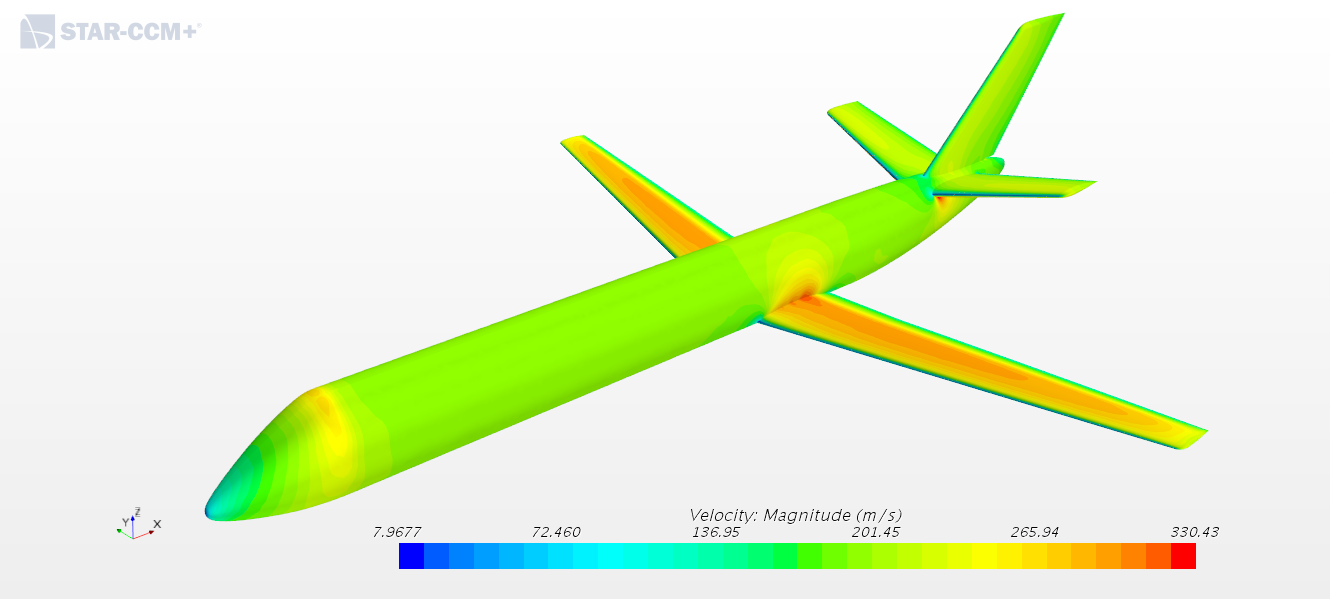
\includegraphics[scale=0.32]{Immagini/Capitolo4/Test_Sim_01_Scalar_Scene_1}
\caption{Velocity magnitude scalar scene for the no-canard configuration}
\label{fig:VMag_01}
\end{figure} 
%
\begin{figure}[H]
\centering
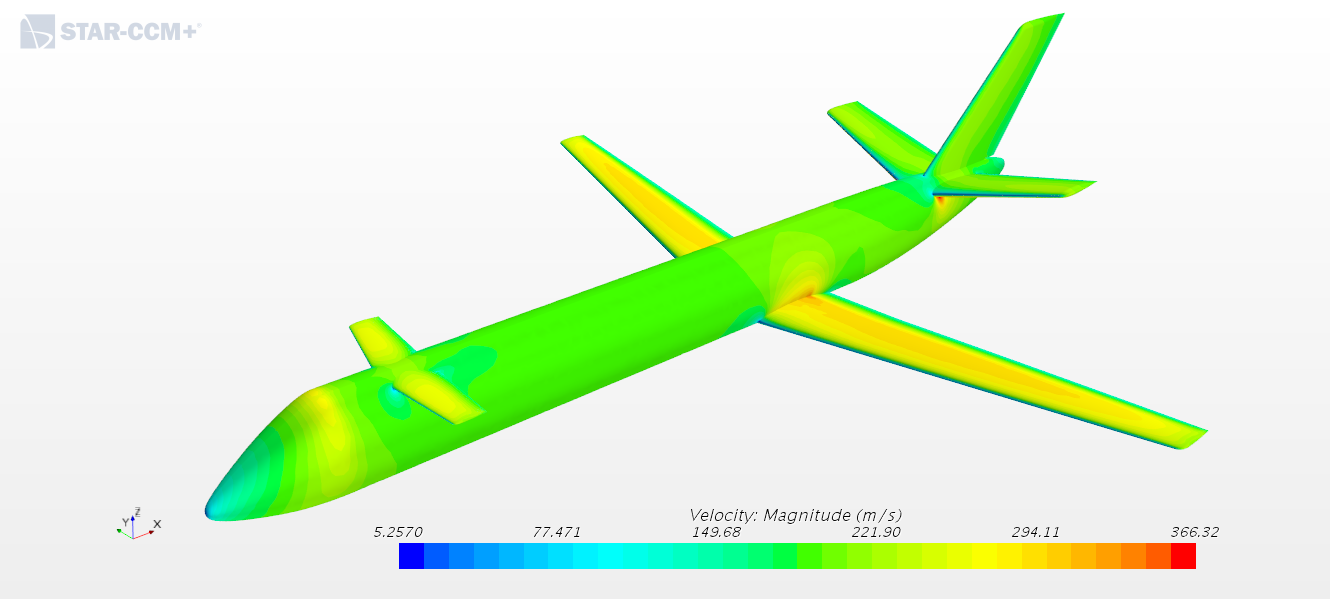
\includegraphics[scale=0.32]{Immagini/Capitolo4/Test_Sim_02_Scalar_Scene_1}
\caption{Velocity magnitude scalar scene for the canard-equipped configuration}
\label{fig:VMag_02}
\end{figure}  
%


\makeatletter
\renewcommand{\bg@material}{}%
\makeatother

% --------------------------------------------------------------------------------------------------------------------------------------------
% APPENDIX
% --------------------------------------------------------------------------------------------------------------------------------------------

\clearpage \phantomsection
\renewcommand{\chaptername}{Appendix}
\renewcommand{\appendixtocname}{Appendices}
\renewcommand{\appendixpagename}{Appendices}
\appendixpage
\noappendicestocpagenum
\addappheadtotoc
\pagestyle{myAppendixPageStyle}

\begin{appendices}
\chapter{Advanced aircraft CAD modeling}
\label{chapApp1}

In Chapter \ref{chap3} the methodologies and the functions used by \gls{JPAD} to model the aircraft main components have been introduced. Altough these methods help to provide a quite satisfactory representation of the aircraft, it is not enough. More effort can be put in trying to produce functions capable to model additional aircraft parts, such as engines, control surfaces and fairings. This appendix just gives an overview of the tests made in this regard, by providing a description of the adopted methodologies and images of the results. It has to be noted that the functions described in the following are still incomplete and require some work before being actually added to the \gls{JPAD} library.

\section{Wing-Fuselage fairing modeling}
\label{secApp1A1}

Several tests have been performed in order to produce a method providing a satisfactory modeling of the wing to fuselage fairing, whatever the position of one relative to the other. Currently, the method allows to generate ventral fairings (located on the underside of the fuselage, between the main wings) and wing to fuselage fairings in case of high wing, even though still more effort needs to be put on this side in order to obtain decent results. For this reason, the following descriptions and figures refer mostly to the first typology. 

\bigskip
\noindent
Since the \gls{JPAD} aircraft classes do not provide a description for the fairings, all the supporting curves have been designed from scratch, generating the points the curves have to pass through (figures \ref{fig:fairing_01} and \ref{fig:fairing_02}) by means of a set of ad hoc parameters. The fairing generator algorithm currently makes use of the following arguments:
%
\begin{itemize}
\renewcommand\labelitemi{\tiny$\blacksquare$}
\renewcommand\labelitemii{\tiny$\bullet$}
\item \textbf{\lstinline[language=Java]!fuselage!} - An instance of the \gls{JPAD} \lstinline[language=Java]!Fuselage! class, providing all the necessary geometric data regarding the fuselage. 
\item \textbf{\lstinline[language=Java]!wing!} - An instance of the \gls{JPAD} \lstinline[language=Java]!LiftingSurface! class, providing all the necessary geometric data regarding the wing, like its position with respect to the fuselage.
\item \textbf{\lstinline[language=Java]!frontLengthFactor!} - A \lstinline[language=Java]!double! quantity fixing how much the fairing extends forward (in the negative $x$ direction) in terms of lifting surface root chord.
\item \textbf{\lstinline[language=Java]!backLengthFactor!} - A \lstinline[language=Java]!double! quantity fixing how much the fairing extends backward (in the positive $x$ direction) in terms of lifting surface root chord.
\item \textbf{\lstinline[language=Java]!sideSizeFactor!} - A \lstinline[language=Java]!double! quantity standing for how large the fairing should be compared to the fuselage diameter, and currently the code does not allow to make the fairing larger than the fuselage. Besides, in case the lifting surface is not detached from the fuselage, there is a minimum side size that the fairing must respect, in order to be sure it \emph{wraps} the lifting surface, which is the fairing main purpose; this limit is automatically imposed by the code.
\item \textbf{\lstinline[language=Java]!fairingHeightFactor!} - A \lstinline[language=Java]!double! quantity that fixes how much the fairing extends above or below: 
%
\begin{itemize}
\item the fuselage, in case the lifting surface is completely contained in it, 
\item the wing, in case the lifting surface upper/lower surface exceeds the limits imposed by the fuselage. 
\end{itemize}
%
The actual height is then calculated in terms of root chord thickness.
\item \textbf{\lstinline[language=Java]!filletRadiusFactor!} - A \lstinline[language=Java]!double! quantity that fixes the radius of the fillet to be applied to the fairing shapes. The actual radius is obtained by multiplying this factor by the distance between the points A and G shown in figure \ref{fig:fairing_01}, in order to make sure the fillet operation can be actually performed, otherwise the fillet algorithm, provided by the \gls{OCCT} library, would encounter some problematics.
\end{itemize}
%
Other two factors are actually provided to the method but they are not as relevant as the aforementioned ones, or, at least, they could be fixed and excluded from the final fairing function arguments list. These factors are the \textbf{\lstinline[language=Java]!heightBelowContactFactor!} and the \textbf{\lstinline[language=Java]!heightAboveContactFactor!}. The contact to which they make reference is the point in which the fairing, with its side size, actually \emph{touches} the fuselage and crosses its surface. Being the fuselage comparable to some sort of cylinder, two contacts point can be actually distinguished. In order to make sure the fairing is correctly shaped, it is necessary it doesn't exceeds some limits fixed by these contact points. Points A and G in figure \ref{fig:fairing_01} are obtained by the use of these factors. In case of ventral fairing, point G $z$ coordinate value is automatically set greater than the one of the lower contact line (how much greater depends on the value of the \lstinline[language=Java]!heightAboveContactFactor!), but less than the one of the upper contact line, in order for the fairing to not exceeds fuselage limits. Point A $z$ coordinate value, instead, is automatically set less than the one of the lower contact line, but greater than the fuselage lower outline one. The values of these factors are just relevant for the fillet actual radius, since the distance between the points A and G is used as a reference lenght for it.
%
\bigskip
\begin{lstlisting}[caption={Fairing CAD method}, captionpos=b, tabsize=2, label={lst:FairingCADMethod}]
public static List<OCCShape> getFairingShapes(
			Fuselage fuselage, 
			LiftingSurface wing,
			double frontLengthFactor,
			double backLengthFactor,
			double sideSizeFactor,
			double fairingHeightFactor,
			double heightBelowContactFactor,
			double heightAboveContactFactor,
			double filletRadiusFactor
			) {
			...
}
\end{lstlisting}
%
\begin{figure}[H]
\centering
\includegraphics[scale=0.50]{Immagini/Appendice/Fairing/fairing_01}
\caption{Ventral fairing root profile curves}
\label{fig:fairing_01}
\end{figure}
%
\begin{figure}[H]
\centering
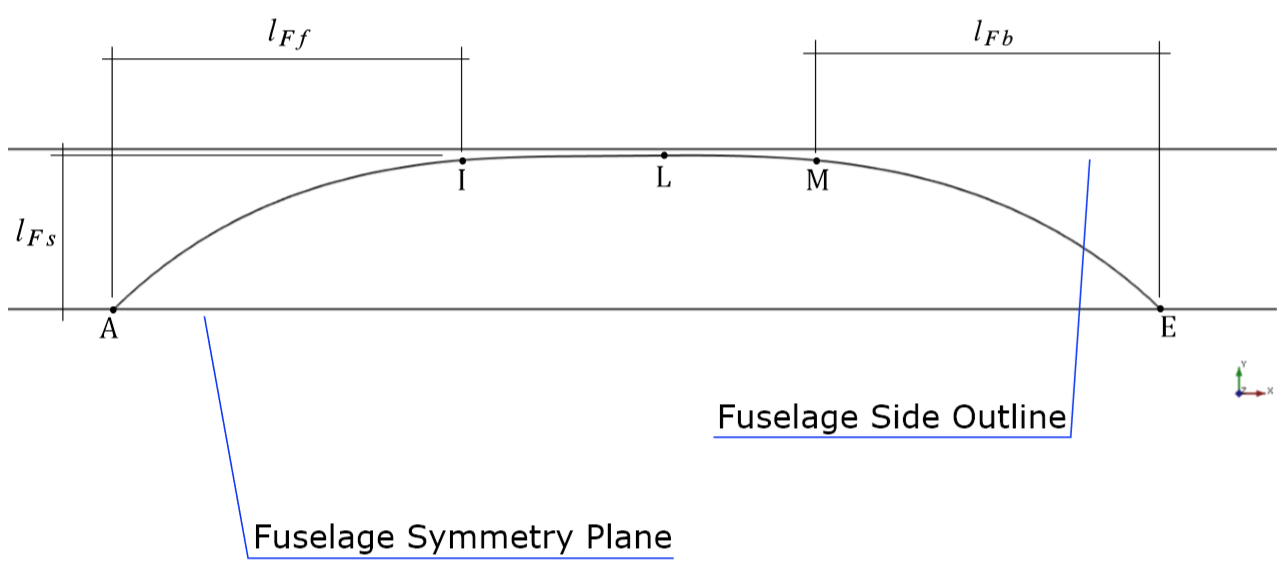
\includegraphics[scale=0.50]{Immagini/Appendice/Fairing/fairing_03}
\caption{Ventral fairing side curve}
\label{fig:fairing_02}
\end{figure}
%  
\bigskip
\begin{table}[H]
\centering
\begin{tabular}{p{1.5cm}p{9.0cm}}
\toprule
\textbf{Length} & \textbf{Description} \\
\midrule
$l_{Ff}$ & The fairing front length, obtained by multiplying the wing root chord by the \lstinline[language=Java]!frontLengthFactor! \\[0.2cm]
$l_{Fb}$ & The fairing back length, obtained by multiplying the wing root chord by the \lstinline[language=Java]!backLengthFactor! \\[0.2cm]
$l_{Fs}$ & The fairing side length, obtained by multiplying half the fuselage width at the wing apex $x$ coordinate by the \lstinline[language=Java]!sideSizeFactor! \\[0.2cm]
$l_{Fh}$ & The fairing height, obtained by multiplying the wing root airfoil thickness by the \lstinline[language=Java]!fairingHeightFactor! \\
\bottomrule
\end{tabular}
\caption{JPAD fairing characteristic lengths}
\label{tab:FairingCharacteristicLengths}
\end{table}
% 

\noindent
By means of the factors listed above, and using the coordinates of the points belonging to the wing root airfoil and the fuselage outlines, the points shown in the previous figures are determined and used in order to generate the wireframe of the fairing. In particular, the side supporting curve depicted in figure \ref{fig:fairing_02} serves as a reference, and is used to build C-shaped elements supporting the following construction of the surfaces belonging to the fairing. In fact, these C-shaped wires, shown in figure \ref{fig:FairingWireframeSupCurves}, extend in the $y$ direction by a quantity provided by the side curve. The edges that form the depicted wires are then used to generate the surfaces of the fairing, by means of the \lstinline[language=Java]!OCCUtils.makePatchThruSections! method (figure \ref{fig:FairingWireframeSupCurves}). It has to be noted that, at this stage, only the right shapes of the fairing are being produced, since the \gls{OCCT} library provides the methods to perform the necessary transformations, as seen in Chapter \ref{chap3}.    
%
\begin{figure}[H]
\centering
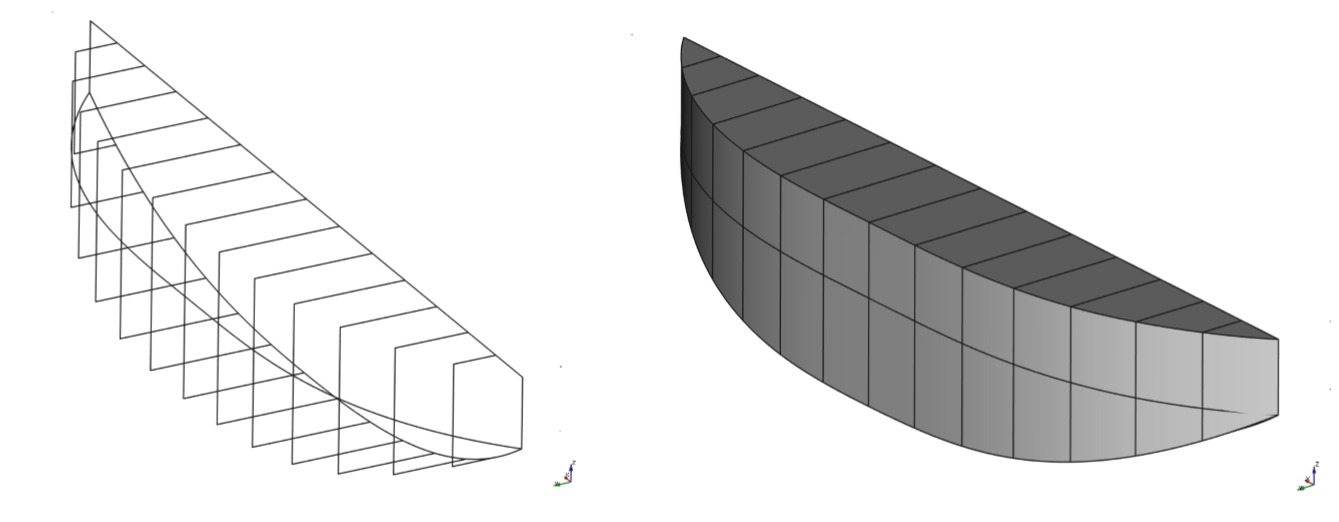
\includegraphics[scale=0.45]{Immagini/Appendice/Fairing/fairing_04}
\caption{Fairing complete wireframe (left) and fairing surfaces (right)}
\label{fig:FairingWireframeSupCurves}
\end{figure}
%  

\bigskip
\noindent
Once the patches on the right side of the fairing have been obtained, they are sewed together by means of the same \gls{OCCT} class used in Chapter \ref{chap3} for the same purpose. The final result is a single shell, onto which a fillet can be applied in order to smooth the edges of the fairing that actually emerge from the fuselage solid. The \gls{OCCT} library provides a class for this operation, called \lstinline[language=Java]!BRepFilletAPI_MakeFillet!, which simply requires the shape on which the operation should be performed, the edge to be smoothed out, and the radius of the fillet. Figure \ref{fig:FairingSolidPlusFillet} shows the final result, once the filleted half fairing shell has been mirrored and the solid has been produced.
%
\begin{figure}[H]
\centering
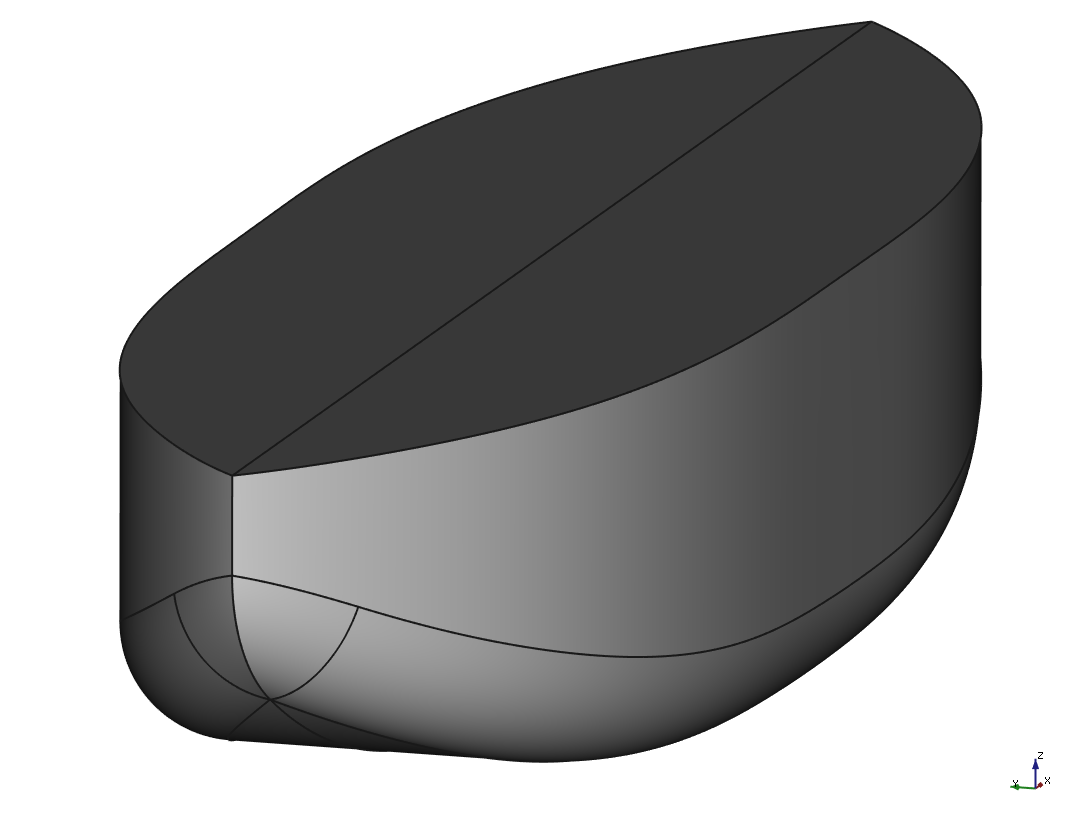
\includegraphics[scale=0.45]{Immagini/Appendice/Fairing/FairingSolidPlusFillet}
\caption{Fairing solid}
\label{fig:FairingSolidPlusFillet}
\end{figure}
%  

\bigskip
\noindent
As mentioned before, the same algorithm can be used to generate different types of fairing. The following pictures show a business aircraft concept equipped with a canard. The function used to generate both the fairings (the one between the canard and the fuselage and the one for the main wing and the fuselage) is exactly the same, with just the values provided to the arguments of the \lstinline[language=Java]!getFairingShapes! function being different (listing \ref{lst:FairingShapes}).
%
\bigskip
\begin{lstlisting}[caption={Fairing CAD method application}, captionpos=b, tabsize=2, label={lst:FairingShapes}]
// Import the aircraft from the XML data file and populate
// JPAD aircraft dedicated classes instances
Aircraft aircraft = AircraftUtils.importAircraft(args);
		
Fuselage fuselage = aircraft.getFuselage();
LiftingSurface wing = aircraft.getWing();
LiftingSurface horTail = aircraft.getHTail();
LiftingSurface verTail = aircraft.getVTail();
LiftingSurface canard = aircraft.getCanard();

// Generate CAD shapes for the aircraft components and the fairings
List<OCCShape> fuselageShapes = getFuselageCAD(
		fuselage, 7, 7, true, true, false);				
List<OCCShape> wingShapes = getLiftingSurfaceCAD(
		wing, ComponentEnum.WING, 1e-3, false, true, false);				
List<OCCShape> wingFairingShapes = getFairingShapes(fuselage, wing,
		1.15, 1.15, 0.50, 0.15, 0.50, 0.50, 0.75);				
List<OCCShape> horTailShapes = getLiftingSurfaceCAD(
		horTail, ComponentEnum.HORIZONTAL_TAIL, 1e-3, false, true, false);				
List<OCCShape> verTailShapes = getLiftingSurfaceCAD(
		verTail, ComponentEnum.VERTICAL_TAIL, 1e-3, false, true, false);				
List<OCCShape> canardShapes = getLiftingSurfaceCAD(
		canard, ComponentEnum.CANARD, 1e-3, false, true, false);				
List<OCCShape> canardFairingShapes = getFairingShapes(fuselage, canard,
		1.50, 0.85, 0.55, 0.20, 0.20, 0.20, 0.75);
\end{lstlisting}
%
\begin{figure}[H]
\centering
\includegraphics[scale=0.80]{Immagini/Appendice/Fairing/fairing_05}
\caption{Canard and main wing to fuselage fairings}
\label{fig:AircraftFairings}
\end{figure}
%  

\section{Control surfaces modeling}
\label{secApp1A2}

Several tests have been performed in order to evaluate the capabilities of the Boolean operations provided by the \gls{OCCT} library, for the purpose of using the same as the main tool to generate control surfaces. \gls{OCCT}, in fact, comes equipped with a package dedicated to Boolean operations, which is \lstinline[language=Java]!BRepAlgoAPI!, that contains \lstinline[language=Java]!BRepAlgoAPI_Cut!, which is the class providing the methods to perform shell/solid cutting operations. The images and the descriptions below mostly refer to the tests made for Fowler type flaps, altough the same Java code, along with the adopted methodologies, can be easily adapted to generate other typologies of flaps and control surfaces in general.

\bigskip
\noindent
The algorithm implemented in the testing classes first requires a solid shape to begin with, which is generated by the use of the \lstinline[language=Java]!getLiftingSurfaceCAD! methods provided by \lstinline[language=Java]!AircraftUtils!, and the geometric data related to the control surface to be produced, such as the breakpoints and the chords. This data is acquired by the means of the \lstinline[language=Java]!get! methods for symmetric/antysimmetric flaps implemented by  \gls{JPAD} \lstinline[language=Java]!LiftingSurface! class. Then, in order to generate the flapped wing, Boolean operations are needed in order to:
%
\begin{enumerate}
\item generate the cut wing, i.e., the wing once cut but with no flaps;
\item generate the flap itself.
\end{enumerate}
%
These operations require the construction of some dedicated solid entities, which need to be designed from scratch using the data regarding the flaps that has been previously acquired. The first of these \emph{cutting} solids are built by using another \lstinline[language=Java]!BRepAlgoAPI! class, which is \lstinline[language=Java]!BRepAlgoAPI_Section!, that produces a section operation between an argument (the wing solid) and tools (vertical planes lineary distributed along the wing). The result of this operation is a set of airfoils, which can be used in order to produce wires to patch through for the purpose of creating the wing cutting solids (figure \ref{fig:WingCuttingWiresPlusSolid})
%
\begin{figure}[H]
\centering
\includegraphics[scale=0.42]{Immagini/Appendice/Flap/flap_05}
\caption{Wing cutting wires (above and left) and wing cutting solids (right) once mirrored}
\label{fig:WingCuttingWiresPlusSolid}
\end{figure}
%  

\bigskip
\noindent
The second set of solids for cutting operations, instead, is produced starting from one of the edges of the wire generated at the previous step, the one that actually intersects the wing shapes. Points are taken on this edge and wires are generated in a similar fashion as the wing cutting ones (figure \ref{fig:FlapCuttingWires}). The solids that result from the patching operation through these wires are used for the flap leading edge adjustment: in fact, the leading edge of the flap must be rounded after the cutting operations for the wing have been performed. This operation could actually be avoided by using the functionalities provided by the \lstinline[language=Java]!BRepFilletAPI_MakeFillet! class instead, as seen for the fairing. But some problems could arise during the filleting operations in case a double edge has been generated at the flap leading edge by the Boolean cut executed on the wing. In order to prevent this possibility, the code performs the rounding of the leading edge of the flap in the aforementioned manner.
%
\begin{figure}[H]
\centering
\includegraphics[scale=0.40]{Immagini/Appendice/Flap/flap_08}
\caption{Flap cutting wire}
\label{fig:FlapCuttingWires}
\end{figure}
%  

\bigskip
\noindent
Once the supporting solids have been produced, Boolean cutting operations can be finally executed. First, cuts are performed on the wing by subtracting wing cutting solids from it one by one. At the end of each cut the argument of the Boolean operation is updated, in order to obtain the so-called cut wing (figure \ref{fig:CutWing}). Turning to the flaps, auxiliary cut wings must be created first (at the center in figure \ref{fig:WingAuxCutWingFlap}). These solids are generated at the same way of the previous ones, but without updating the argument of the Boolean operation, so that it stays equal to the original wing. Then the auxiliary cut wings are subtracted one by one from the wing, in order to obtain the flaps, whose leading edge is adjusted by means of the aforementioned flap cutting solids (figure \ref{fig:FlapLEAdjustment}).
%
\begin{figure}[H]
\centering
\includegraphics[scale=0.52]{Immagini/Appendice/Flap/WingCutSolid_04}
\caption{Cut wing}
\label{fig:CutWing}
\end{figure}
%
\begin{figure}[H]
\centering
\includegraphics[scale=0.50]{Immagini/Appendice/Flap/flap_07}
\caption{Flap generation steps}
\label{fig:WingAuxCutWingFlap}
\end{figure}  
%
\begin{figure}[H]
\centering
\includegraphics[scale=0.35]{Immagini/Appendice/Flap/FlapPlusFlapCuttingSolid_01}
\caption{Flap leading edge adjustment}
\label{fig:FlapLEAdjustment}
\end{figure}
%  

\bigskip
\noindent
The final step consists in moving the flaps with respect to the cut wing. As mentioned before, the \gls{OCCT} library provides also the classes to perform transformations such as translation and rotation. However, it has to be noted that the current algorithm for control surfaces motion still needs some work and adjustment, especially regarding the Fowler flaps. The following figures show the final result for different wings. In particular, figures \ref{fig:ATR72Fowler} and \ref{fig:CS300Fowler} show the wings of the ATR-72 and CS300 respectively, equipped with inboard and outboard Fowler flaps. Figure \ref{fig:TailControlSurfaces}, instead, shows the horizontal and vertical stabilizers of the ATR-72, equipped with elevator and rudder treated as plain flaps.
%
\begin{figure}[H]
\centering
\includegraphics[scale=0.50]{Immagini/Appendice/Flap/flap_09}
\caption{ATR-72 wing, with inboard and outboard Fowler flaps}
\label{fig:ATR72Fowler}
\end{figure}
%
\begin{figure}[H]
\centering
\includegraphics[scale=0.50]{Immagini/Appendice/Flap/flap_10}
\caption{CS300 wing, with inboard and outboard Fowler flaps}
\label{fig:CS300Fowler}
\end{figure}
%
\begin{figure}[H]
\centering
\includegraphics[scale=0.50]{Immagini/Appendice/Flap/flap_11}
\caption{ATR-72 tail, with rotated elevator and rudder}
\label{fig:TailControlSurfaces}
\end{figure}
%
\chapter{Importing CAD models into a JavaFX window}
\label{chapApp2}

\gls{JPAD} comes equipped with a simple yet very intuitive \gls{acr:GUI}, which provides the user with the possibility to import aircraft data in several ways and perform analyses. Altough the \gls{JPAD} \gls{acr:GUI} currently offers different 2D views of the aircraft (made mostly from the outlines of each of the aircraft components), allowing the user to check the actual configuration and realize quite instantly the changes made to it after modifying some of the available parameters, it would be quite interesting and useful to give also the possibility to view the 3D model of the aircraft, built by means of the \lstinline[language=Java]!JPADCAD! package and the utility functions contained in \lstinline[language=Java]!AircraftUtils!.

\bigskip
\noindent
The Java language offers the possibility to design and create applications such as a simple window for 3D models view and exploration by means of the JavaFX platform \cite{JavaFXPlatform}. JavaFX is a Java library that can be used to build complex applications, that can run consistently across multiple platforms and on various devices, such as desktop computers, mobile phones, TVs, tablets, etc. In general, a JavaFX application has three major components, namely \emph{Stage}, \emph{Scene}, and \emph{Nodes}. The stage (a window) contains all the objects of a JavaFX application, and is represented by the \lstinline[language=Java]!Stage! class. The primary stage is automatically created by the platform itself and is passed as an argument to the \lstinline[language=Java]!start! method of the \lstinline[language=Java]!Application! class, the abstract class from which all the JavaFX applications extend. A scene, instead, represents the physical contents of a JavaFX application. It contains the \emph{Scene Graph}, which is a tree-like data structure, whose root, branches, and leaves are represented by nodes. A node, in general, may include:
%
\begin{itemize}
\item geometrical objects, such as circles, rectangles, polygons, etc.;
\item controls, such as buttons, check box, choice box, text area, etc.;
\item containers, such as border pane, grid pane, flow pane, etc.;
\item media elements, such as audio, video, and image objects.
\end{itemize}
%
A branch node (also called parent node) is a node with child nodes. There are several types of parent nodes, the most used of which is the \emph{Group} one. A group node is a collective node and whenever the group node is rendered, all its child nodes are rendered in order. Any transformation applied on the group is applied to all the child nodes.

\bigskip
\noindent
The objects that we want to import into a JavaFX window are much more complicated than the ones that can be created by using the three built-in 3D shape classes that come with JavaFX: \lstinline[language=Java]!Cylinder!, \lstinline[language=Java]!Box!, and \lstinline[language=Java]!Sphere!. For more complex objects, the JavaFX library provides the user with the \lstinline[language=Java]!TriangleMesh! class, which allows to create objects based on a connected series of triangles. In order to create the necessary \lstinline[language=Java]!TriangleMesh! objects, which should represent the 3D shapes of the aircraft obtained by the use of \lstinline[language=Java]!JPADCAD!, it is crucial some sort of conversion from \lstinline[language=Java]!TopoDS_Shape! (the generic \gls{OCCT} class managing all sort of shapes) to \lstinline[language=Java]!TriangleMesh! entities. \lstinline[language=Java]!OCCDataProvider! and \lstinline[language=Java]!OCCFXMeshExtractor! are the \lstinline[language=Java]!JPADCAD! classes providing the instruments for this operation. In particular, to generate a \lstinline[language=Java]!TriangleMesh! instance three collections must be defined: one for the points, one for the faces, and one for the texture coordinates. The \lstinline[language=Java]!OCCFXMeshExtractor! class, along with its \lstinline[language=Java]!FaceData! sub-class (which extends the generic \lstinline[language=Java]!OCCDataProvider! one), allows to automatically convert \lstinline[language=Java]!TopoDS_Face! objects to \lstinline[language=Java]!TriangleMesh! entities, by employing the face object underlying mesh data structure (handled by the \gls{OCCT} \lstinline[language=Java]!BRepMesh_IncrementalMesh! class). In this way, the aircraft 3D model (its face-type shapes) can be converted into a list of sub-lists of \lstinline[language=Java]!TriangleMesh! entities, with each sub-list being relative to a particular aircraft component (listing \ref{lst:FaceConversion}).
%
\bigskip
\begin{lstlisting}[caption={Solid shapes conversion to JavaFX triangle meshes}, captionpos=b, tabsize=2, label={lst:FaceConversion}]
// Import the aircraft into the application
Aircraft theAircraft = AircraftUtils.importAircraft(args);

// Generate selected aircraft solid shapes
List<ComponentEnum> comps = new ArrayList<>();
comps = Arrays.asList(new ComponentEnum[] {
		ComponentEnum.FUSELAGE, 
		ComponentEnum.WING, 
		ComponentEnum.HORIZONTAL_TAIL, 
		ComponentEnum.VERTICAL_TAIL, 
		ComponentEnum.CANARD
});

List<OCCShape> allShapes = AircraftUtils.getAircraftShapes(theAircraft, comps);
List<TopoDS_Solid> solids = AircraftUtils.getAircraftSolid(allShapes);
		
// Extract the triangle meshes
List<List<TriangleMesh>> triangleMeshes = solids.stream()
	.map(s -> (new OCCFXMeshExtractor(s)).getFaces().stream()
		.map(f -> {
			FaceData faceData = new FaceData(f, true);
			faceData.load();
			return faceData.getTriangleMesh();
		})
		.collect(Collectors.toList()))
	.collect(Collectors.toList());
\end{lstlisting}
%

\bigskip
\noindent
The converted faces are then added to a group, after being given a specific color based on the aircraft surface they belong to. This group, in turn, is added to another one, which acts as a camera for the final scene. The result is shown in the following figure, which depicts four different aircrafts imported into a JavaFX window by the means of the same application. The next step, obviously, will consist in adding the so-created window to the \gls{JPAD} \gls{acr:GUI}.
%
\begin{figure}[H]
\centering
\includegraphics[scale=0.51]{Immagini/Appendice/javafx_01}
\caption{\lstinline[language=Java]!JPADCAD! aircrafts imported into the JavaFX application}
\label{fig:javafx_01}
\end{figure}
% 
\end{appendices}

% --------------------------------------------------------------------------------------------------------------------------------------------
% BIBLIOGRAPHY
% --------------------------------------------------------------------------------------------------------------------------------------------

\clearpage \phantomsection
\addcontentsline{toc}{chapter}{Bibliography}
\pagestyle{myBibliographyPageStyle}
\nocite{*}
\printbibliography[heading=myBibliography]

% --------------------------------------------------------------------------------------------------------------------------------------------
% GLOSSARY, ACRONYMS, SYMBOLS
% --------------------------------------------------------------------------------------------------------------------------------------------

\glsaddall
\glossarystyle{list}

\markboth{}{}
\clearpage
\pagestyle{myGlossaryPageStyle}
\printglossary[type=main]

\markboth{}{}
\clearpage
\pagestyle{myAcronymsPageStyle}
\printglossary[type=\acronymtype]

%\markboth{}{}
%\clearpage
%\pagestyle{myListOfSymbolsPageStyle}
%\printglossary[type=symbols]

% --------------------------------------------------------------------------------------------------------------------------------------------
% END DOCUMENT
% --------------------------------------------------------------------------------------------------------------------------------------------

\end{document}

